% Options for packages loaded elsewhere
\PassOptionsToPackage{unicode}{hyperref}
\PassOptionsToPackage{hyphens}{url}
%
\documentclass[
]{article}
\usepackage{amsmath,amssymb}
\usepackage{iftex}
\ifPDFTeX
  \usepackage[T1]{fontenc}
  \usepackage[utf8]{inputenc}
  \usepackage{textcomp} % provide euro and other symbols
\else % if luatex or xetex
  \usepackage{unicode-math} % this also loads fontspec
  \defaultfontfeatures{Scale=MatchLowercase}
  \defaultfontfeatures[\rmfamily]{Ligatures=TeX,Scale=1}
\fi
\usepackage{lmodern}
\ifPDFTeX\else
  % xetex/luatex font selection
\fi
% Use upquote if available, for straight quotes in verbatim environments
\IfFileExists{upquote.sty}{\usepackage{upquote}}{}
\IfFileExists{microtype.sty}{% use microtype if available
  \usepackage[]{microtype}
  \UseMicrotypeSet[protrusion]{basicmath} % disable protrusion for tt fonts
}{}
\makeatletter
\@ifundefined{KOMAClassName}{% if non-KOMA class
  \IfFileExists{parskip.sty}{%
    \usepackage{parskip}
  }{% else
    \setlength{\parindent}{0pt}
    \setlength{\parskip}{6pt plus 2pt minus 1pt}}
}{% if KOMA class
  \KOMAoptions{parskip=half}}
\makeatother
\usepackage{xcolor}
\usepackage{longtable,booktabs,array}
\usepackage{calc} % for calculating minipage widths
% Correct order of tables after \paragraph or \subparagraph
\usepackage{etoolbox}
\makeatletter
\patchcmd\longtable{\par}{\if@noskipsec\mbox{}\fi\par}{}{}
\makeatother
% Allow footnotes in longtable head/foot
\IfFileExists{footnotehyper.sty}{\usepackage{footnotehyper}}{\usepackage{footnote}}
\makesavenoteenv{longtable}
\setlength{\emergencystretch}{3em} % prevent overfull lines
\providecommand{\tightlist}{%
  \setlength{\itemsep}{0pt}\setlength{\parskip}{0pt}}
\setcounter{secnumdepth}{-\maxdimen} % remove section numbering
\ifLuaTeX
  \usepackage{selnolig}  % disable illegal ligatures
\fi
\IfFileExists{bookmark.sty}{\usepackage{bookmark}}{\usepackage{hyperref}}
\IfFileExists{xurl.sty}{\usepackage{xurl}}{} % add URL line breaks if available
\urlstyle{same}
\hypersetup{
  hidelinks,
  pdfcreator={LaTeX via pandoc}}

\author{}
\date{}


% --- SHADOWRUN 7E CUSTOM STYLING ---
% Typography & Layout
\usepackage[margin=0.75in]{geometry}
\usepackage{multicol}
\usepackage{helvet} % Sans-serif clean font
\renewcommand{\familydefault}{\sfdefault}
\usepackage{microtype}

% Structural Spacing & Formatting
\usepackage{parskip}   % Remove paragraph indents, add vertical space
\usepackage{enumitem}  % Control list spacing
\setlist{nosep}        % Make all lists compact by default

% Game Term Styling (No math-mode for crunch)
\newcommand{\gameterm}[1]{\textbf{\sffamily #1}}

% Colors
\definecolor{matrixblue}{HTML}{00CCFF} % Neon blue for HUD elements
\definecolor{srdark}{HTML}{1A1A1A}     % Deep charcoal for JackPoint backgrounds
\definecolor{sraccent}{HTML}{E63946}   % Warning/Glitch red

% Headers and Footers (HUD Style)
\usepackage{fancyhdr}
\pagestyle{fancy}
\fancyhf{}
\renewcommand{\headrulewidth}{0pt}
\renewcommand{\footrulewidth}{1.5pt}
\renewcommand{\footrule}{\hbox to\headwidth{\color{matrixblue}\leaders\hrule height \footrulewidth\hfill}}
\fancyfoot[L]{\ttfamily\small SYSTEM STATUS: ONLINE \textbar{} GRID LOCATION: OKC-METRO}
\fancyfoot[R]{\ttfamily\small PAGE \thepage}

% Watermark
\usepackage[pages=all]{background}
\backgroundsetup{
  scale=1,
  color=black,
  opacity=0.05,
  angle=0,
  position=current page.center,
  vshift=0pt,
  hshift=0pt,
  contents={%
  \begin{tikzpicture}[remember picture,overlay]
    \draw [step=0.5cm,line width=0.5mm]
      (current page.south west) grid (current page.north east);
  \end{tikzpicture}%
  }
}

% Chapter Headings (Tight Spacing)
\usepackage{titlesec}
\titleformat{\section}[block]
  {\normalfont\LARGE\bfseries\color{matrixblue}\MakeUppercase}
  {\thesection}{1em}{}
  [\vspace{0.5ex}\color{matrixblue}\titlerule\vspace{0.25ex}\color{sraccent}\titlerule]
\titlespacing*{\section}{0pt}{1.5ex plus 1ex minus .2ex}{1ex plus .2ex}

\titleformat{\subsection}[block]
  {\normalfont\Large\bfseries\color{srdark}\MakeUppercase}
  {\thesubsection}{1em}{}
  [\color{matrixblue}\titlerule]
\titlespacing*{\subsection}{0pt}{1.2ex plus 1ex minus .2ex}{0.8ex plus .2ex}

\titleformat{\subsubsection}[block]
  {\normalfont\large\bfseries\color{srdark}\MakeUppercase}
  {\thesubsubsection}{1em}{}
  [\color{matrixblue}\titlerule]
\titlespacing*{\subsubsection}{0pt}{1ex plus 1ex minus .2ex}{0.5ex plus .2ex}

% Tables
\usepackage{tabularray}
\UseTblrLibrary{booktabs}

% Callout Boxes
\usepackage[most]{tcolorbox}

% The JackPoint Commentary Box
\newtcolorbox{jackpoint}[2][]{
    enhanced,
    colback=srdark,
    colframe=matrixblue,
    coltext=white,
    boxrule=0.5pt,
    leftrule=4pt, % Thick accent line on the left
    arc=0mm,      % Sharp, digital corners
    fonttitle=\bfseries\ttfamily\small,
    title={>> USER: #2 <<},
    attach title to upper,
    after title={\par\vspace{0.5em}\hrule\vspace{0.5em}},
    #1
}

% GM Advice Box
\newtcolorbox{gmadvice}[1][GM Advice]{
  colback=gray!10,
  colframe=sraccent,
  coltitle=white,
  fonttitle=\bfseries\MakeUppercase,
  title={#1},
  boxrule=1.5pt,
  leftrule=4pt,
  arc=0mm,
  coltext=black
}
% --- END SHADOWRUN 7E CUSTOM STYLING ---

% Custom Gear Entry Macro
\newcommand{\gearitem}[3]{%
  \noindent\textbf{\textcolor{matrixblue}{#1}} #2%
  \ifx&#3&\else\\ \textit{\textcolor{gray!80}{#3}}\fi
  \par\vspace{1em}%
}


\begin{document}
\begin{multicols}{2}


\textbf{Fan made Shadowrun 7th Edition}

\hypertarget{shadowrun-7th-edition-homebrew-the-merged-world}{%
\subsection{Shadowrun 7th Edition Homebrew: The Merged
World}\label{shadowrun-7th-edition-homebrew-the-merged-world}}

The confluence of eldritch power and frighteningly advanced technology
has forcibly merged the Matrix with the gaiasphere. The grey goo ate the
world and spit it back out. Welcome to the 6th World, where everything
has an AR signature and magic is bleeding into the code.

\hypertarget{i.-core-mechanics-dice-tests}{%
\subsubsection{I. Core Mechanics: Dice \&
Tests}\label{i.-core-mechanics-dice-tests}}

All actions use a streamlined success-counting system.

\begin{itemize}

\item
  \textbf{Dice Pool:} Attribute + Skill.
\item
  \textbf{Hits:} All tests use six-sided dice (D6). A result of
  \textbf{5 or 6} is a Hit.
\item
  \textbf{Glitches:} If more than half the dice rolled are \textbf{1s},
  you Glitch (a complication occurs). If you Glitch with 0 hits, it's a
  \textbf{Critical Glitch} (catastrophe).
\item
  \textbf{Rule of 6 (Ro6):} When applicable (e.g., using Edge), a rolled
  6 counts as a hit and is rolled again.
\item
  \textbf{Wild Dice:} Used in high-mana or nanite-saturated areas. Roll
  these with a different colored die. A \textbf{6} counts as \textbf{3
  hits} (and explodes if Ro6 applies). However, a \textbf{1} cancels all
  standard \textbf{5s} rolled in that pool.
\end{itemize}

\begin{center}\rule{0.5\linewidth}{0.5pt}\end{center}

\hypertarget{ii.-the-matrix-the-gaiasphere}{%
\subsubsection{II. The Matrix \& The
Gaiasphere}\label{ii.-the-matrix-the-gaiasphere}}

The Matrix is no longer separate from reality; it is a nanite-infused
environment. Even the hermit in the woods is lit up with an AR signature
because the water and air are crawling with nanites.

\begin{itemize}

\item
  \textbf{No Cold Sim (The Abyss Looks Back):} Cold Sim is dead. Any
  active skill involving the Matrix requires a Direct Neural Interface
  (DNI), and all DNI connections are Hot Sim. You put your brain and
  soul on the line. Acting in AR without DNI limits your dice pools to
  the flat stats of your commlink or cyberdeck.
\item
  \textbf{Aspected Noise:} Distinct corporate grids are gone. ``Noise''
  now acts exactly like a magical Background Count. It has surges,
  voids, and aspects (Matrix Ley Lines) that can provide \textbf{Wild
  Dice} or severe penalties depending on the local grid.
\item
  \textbf{Ritual Hacking:} Remote hacking without a direct connection
  functions like Ritual Spellcasting. Personal data (SINs, biometric
  data, deeply personal secrets) acts as a sympathetic ``material
  link.'' The older the data, the more the link degrades.
\end{itemize}

\hypertarget{updated-matrix-actions-tethers-g.o.d.}{%
\paragraph{Updated Matrix Actions: Tethers \&
G.O.D.}\label{updated-matrix-actions-tethers-g.o.d.}}

\begin{itemize}

\item
  \textbf{Tethers (Replacing Marks):} Marks act like sympathetic bonds.
  Placing a Tether on a device/persona requires an Opposed Test
  (\emph{Logic + Hacking vs.~Willpower + Firewall}). Each Tether gives
  +1 Die on subsequent actions against them. \emph{Warning:} If you
  Glitch while exploiting a Tether, the two-way connection gives the
  target a free blast of Biofeedback against you.
\item
  \textbf{G.O.D. Manifestations:} Grid Overwatch is now a localized,
  immune-system response from the merged gaiasphere. Instead of a flat
  timer, when a hacker rolls a \textbf{1 on a Wild Die} during a Matrix
  action, it summons a G.O.D. manifestation (a lethal Sprite/Spirit
  hybrid) directly to their digital location.
\end{itemize}

\begin{center}\rule{0.5\linewidth}{0.5pt}\end{center}

\hypertarget{iii.-magic-resonance-and-the-soul}{%
\subsubsection{III. Magic, Resonance, and the
Soul}\label{iii.-magic-resonance-and-the-soul}}

Consciousness equals a soul. The line between flesh and data is
permanently blurred, but Tech and Magic still ruthlessly repel each
other.

\begin{itemize}

\item
  \textbf{Digital Essence (Turing 1, Searle 0):} Any AI, Sprite, or
  Matrix entity complex enough to possess a self-directed persona has an
  \textbf{Essence of 6}, an Aura, and counts as a living being. They are
  vulnerable to Essence Drain and can grow or heal Essence just like
  metahumans. Digital Essence acts exactly like metahuman Essence for
  the purposes of social interaction and determining the entity's
  baseline willpower. Should a digital entity lose Essence (e.g.~through
  traumatic data loss or being subjected to Essence Drain), they suffer
  penalties to their mental attributes and social tests, reflecting
  their fading identity. Losing all 6 Essence means the entity has been
  reduced to mindless, fragmented code and is destroyed.
\item
  \textbf{Essence Growth:} Essence is not just what you are born with;
  it is who you are and what you become. Lost essence can be regained
  through Karma, roleplay, and character growth.
\item
  \textbf{Oil and Water:} Tech and magic are in contact, but they do not
  mix. No entity can \emph{ever} possess both a Magic (MAG) and
  Resonance (RES) attribute simultaneously.
\item
  \textbf{Background Count (BC) \& The Wild Edge:} The normal BC of
  Seattle fluctuates between 1--6 (GM rolls 1D6). When casting in a
  positive BC, you substitute a number of dice in your pool with
  \textbf{Wild Dice} equal to the BC level. You may also Overcast a
  spell by adding its Force up to the BC level, adding 1 to the Drain
  Value for every Force level above your MAG rating.
\end{itemize}

\begin{center}\rule{0.5\linewidth}{0.5pt}\end{center}

\hypertarget{iv.-spirits-sprites-and-hybrid-entities}{%
\subsubsection{IV. Spirits, Sprites, and Hybrid
Entities}\label{iv.-spirits-sprites-and-hybrid-entities}}

With the veil parted, digital and astral entities interact in entirely
new ways.

\begin{itemize}

\item
  \textbf{Manifesting Sprites:} Sprites can physically manifest by
  swarming nanites into a dense ball, literally munching ambient
  physical matter to build a temporary shell. The smarter the Sprite,
  the harder it is for a Technomancer to control.
\item
  \textbf{Crystalline Spirits:} These ancient spirits of order transmute
  matter into ``living crystal.'' They act as a magical ``bootloader,''
  allowing AIs to manifest a physical presence and an astral aura.
\item
  \textbf{Possession vs.~Inhabitation:}
\item
  \emph{Possession (The Joyride):} A spirit/entity takes temporary
  control of a host. The host's original stats (including RES) are
  suppressed but not destroyed.
\item
  \emph{Inhabitation (The Merger):} A permanent, violent merging
  creating a dual-natured hybrid. If a spirit Inhabits a Technomancer,
  the host's Resonance stat is permanently destroyed (reduced to 0 due
  to the Oil and Water rule), though the spirit retains the host's
  physical skills.
\end{itemize}

\begin{center}\rule{0.5\linewidth}{0.5pt}\end{center}

\hypertarget{v.-character-creation-summary}{%
\subsubsection{V. Character Creation
Summary}\label{v.-character-creation-summary}}

All characters build and advance using \textbf{Karma}.

\end{multicols}
\begin{longtable}[]{@{}
  >{\raggedright\arraybackslash}p{(\columnwidth - 4\tabcolsep) * \real{0.3333}}
  >{\raggedright\arraybackslash}p{(\columnwidth - 4\tabcolsep) * \real{0.3333}}
  >{\raggedright\arraybackslash}p{(\columnwidth - 4\tabcolsep) * \real{0.3333}}@{}}
\toprule\noalign{}
\begin{minipage}[b]{\linewidth}\raggedright
Special Quality
\end{minipage} & \begin{minipage}[b]{\linewidth}\raggedright
Karma Cost
\end{minipage} & \begin{minipage}[b]{\linewidth}\raggedright
Primary Benefit
\end{minipage} \\
\midrule\noalign{}
\endhead
\bottomrule\noalign{}
\endlastfoot
\textbf{Magician} & 100 & Access to all magical skills; gains 2x MAG
free spells. \\
\textbf{Technomancer} & 80 & Access to Resonance; gains 2x RES Complex
Forms. \\
\textbf{Adept} & 75 & Free Power Points equal to MAG rating. \\
\textbf{Aspected Magician} & 50 & Specialized focus; gains 3x MAG free
spells. \\
\textbf{Mystic Adept} & 150 & Blends Adept and Magician traits; gains 1x
MAG free spells. \\
\end{longtable}
\begin{multicols}{2}

\emph{(Note: Magic and Resonance both start at 0. You must buy one of
these qualities at character generation to unlock the stat, which starts
at Rating 1).}

\begin{enumerate}
\def\labelenumi{\arabic{enumi}.}

\item
  \protect\hyperlink{bookmark=id.x87h504b24hr}{Dice \& Tests}\\
\item
  \protect\hyperlink{bookmark=id.kkav13e62x7p}{Character Creation \&
  Advancement}\\
\item
\end{enumerate}

\textbf{Dice \& Tests}

\textbf{To Hit, or to Glitch:}

Every \textbf{Action} taken by a character that is important to the
narrative, or an Action that is difficult beyond an everyday, normal
encounter requires a \textbf{Test} to see if it succeeds or fails.
Similarly, any Action that is opposed by another character, or an Action
that could potentially have negative consequences requires a Test.
Common, everyday occurrences do not require rolling any dice. At GM
discretion, any Action that is trivially within your skillset requires
no Test.\\
A Test's success or failure is measured by rolling a number of dice
equal to the \textbf{Dice Pool} for the task at hand. Generally this
Dice Pool takes the form of the relevant \textbf{Skill} rating and its
\textbf{Linked Attribute} rating. All dice used are six sided, D6, and
count as a \textbf{Hit} if rolled as a 5 or a 6. The more Hits rolled
the more likely you are to succeed, or the more impactful your success
may be. \textbf{Dice Pool Modifiers} from gear, spells, abilities, or
the environment may raise or lower the number of dice in the Dice Pool
for any given task. When a die result is anything other than a 5 or a 6,
it is a \textbf{miss}. Normally rolling many misses has no effect; you
may still have enough Hits to succeed. However, if more than half of the
dice results are a 1 then you \textbf{`Glitch'}. When a Glitch occurs
something bad happens to inconvenience your character at the GM's
discretion; dropping your gun, falling off balance, etc. It is possible
to both succeed at a Test by rolling enough Hits and Glitch by rolling
more than half 1's simultaneously; \emph{e.g.: you succeed at punching
your target, but you overextend throwing the punch so hard that you slip
and fall in the process}.

\textbf{Critical Glitch:}

If you Glitch on a Test and do not roll a single Hit then you have made
a \textbf{Critical Glitch}. A Critical Glitch is a serious mishap or
setback, potentially even damaging or life threatening to the character.
Some examples would include your gun exploding in your hand on a
misfire, your brakes malfunctioning during a high speed chase, or
miraculously throwing the pin while keeping hold of the grenade.
Critical Glitches should not always result in instant character death,
and they can be downgraded with the use of \textbf{Edge}.

\textbf{Buying Hits:}

For every 4 dice available in your Dice Pool you may buy 1 automatic Hit
on a Test instead of making a roll. If the Test is significant and a
potential failure or Glitch could change the course of play, the GM may
disallow buying hits for that Test. Buying Hits may not be combined with
rolling dice; you may NOT spend part of your Dice Pool on buys and roll
the remainder.

\textbf{Thresholds:}

The \textbf{Threshold} for a Test is the number of Hits required to
succeed. Any extra Hits rolled above the Threshold's requirement become
\textbf{Net Hits}. Net Hits can result in more damage in combat or other
positive effects, at GM discretion. Unless stated in the rules for a
specific Action or listed as a Derived Threshold for an NPC Opposed
Test, the GM determines what the Threshold, or difficulty, is for each
individual Test.

\textbf{Test Types:}

The normal \textbf{Success Test} for most Actions involves a simple Dice
Pool consisting of the relevant Skill rating, the Linked Attribute
rating, and the GM's stated difficulty, or Threshold. \emph{E.g.: A
player with Athletics rating 4 and Strength rating 4 is attempting to
swim upriver against a strong current. The GM determines their Threshold
for the Test is a 4 and they roll a total of 3 Hits from their 8 dice;
they have failed the Test}.

Success Test = Attribute + Skill (Threshold)

Another type of Test is an \textbf{Extended Test}, which allows you to
roll your Dice Pool multiple times until you have accumulated enough
Hits to meet the Threshold. This Test adds an \textbf{Interval}
representing how much time is required for each roll of the dice, or how
much time must pass between attempts. Extended Tests are usually
something you will succeed at eventually, unless you run out of time or
encounter something that prevents you from continuing. Glitches on an
Extended Test will reduce the accumulated number of Hits by 1D6; if the
number of Hits is reduced to 0 the Test fails. Critically Glitching on
an Extended Test automatically fails the Test in addition to
consequences the GM determines. When an Extended Test fails you must
completely restart to attempt it again; this also means replacing any
required materials or resources that were expended in the first
attempt.\\
Extended Tests can be rushed and their listed Interval halved, but doing
so counts all 1's and 2's rolled for determining if a Glitch or Critical
Glitch has occurred.

Extended Test = Attribute + Skill (Threshold, Interval)

When an Action is actively opposed by another character an
\textbf{Opposed Test} is required. This is treated the same as a Success
Test, but in place of a Threshold the opposing character rolls their own
Dice Pool and the Hits from each are compared. Whichever side rolls more
Hits wins and the excess Hits they rolled become Net Hits.

Opposed Test = Attribute + Skill (target's Attribute + Skill) When
opposed by a NPC it is advised to use the \textbf{NPC Opposed Test} in
the interests of speeding up gameplay. This pits the character's Dice
Pool against the NPC's \textbf{Derived Threshold} or difficulty rating
instead of rolling a Dice Pool and tallying Hits for the NPC. This Test
can also be used when a character is the target of a NPC Action, pitting
the NPC's difficulty rating or Derived Threshold against a character's
opposing Dice Pool.

NPC Opposed Test = Attribute + Skill (NPC rating)

NPC Opposed Test = NPC rating (Attribute + Skill)

The GM may call for an \textbf{Attribute Test} in some circumstances.
This may be a single Attribute rolled against a threshold, \emph{e.g.:
using Strength to force a door open}. Some physical or mental
capabilities of a character may be derived from two Attributes instead
of forming the Dice Pool from an Attribute + a Skill.

Attribute Test = Attribute (Threshold)

A \textbf{Composure Test} is used to overcome emotionally strenuous or
dangerous and frightening situations. It is also used by characters to
resist many types of compulsions or instinctive reactions.

Composure Test = CHA + WIL (Threshold)

When a character needs to know their gut instinct or questions if they
can trust others, an opposed \textbf{Judge Intentions Test} may be made
at GM discretion, usually when directly in a conversation or physically
near the target character.

Judge Intentions Test = CHA + INT (target's WIL + CHA)

Attempting to lift or carry a large weight may require a
\textbf{Lift/Carry Test}. Characters may normally lift a weight equal to
their STR x 15 kg without any Test required; a weight beyond this
requires a successful Lift/Carry Test with each hit increasing the
weight you may lift by an additional 15 kg. Lifting weight above your
head requires more effort, dropping the normal limit to STR x 5 kg and
increasing by 5 kg with each hit on the Lift/Carry Test. Carrying heavy
items beyond your immediate reach uses a baseline of STR x 10 kg and a
10 kg increase with each hit.

Lift/Carry Test = BOD + STR

Any time a character attempts to memorize something, or to later recall
that information, they must make a \textbf{Memory Test}. All hits scored
to memorize add dice later to a \textbf{Recall Test} for recalling that
info. Be sure that you or the GM record the number of hits. You may not
make additional Memory Tests on the same object, word, image, thought,
or concept to stack up this dice bonus. Memory Test = LOG + WIL

Recall Test = LOG + WIL (Threshold)

\textbf{Trying Again:}

If you fail a Success Test or Extended Test and other circumstances do
not prevent doing so, you are welcome to try again. Each successive
attempt incurs a -2 dice pool modifier unless the GM deems you have
spent enough time taking a break between attempts. This penalty is never
applied to Opposed Tests.

\textbf{Teamwork:}

More than one character can attempt a Test together as a
\textbf{Teamwork Test}. One character is designated the leader; all
others are helpers and roll their dice pools as they normally would if
they were attempting the Action alone. Any net hits scored by the
helpers become bonus dice for the leader's dice pool, who then attempt
the Test per normal rules. GM discretion applies to what can or can't be
helped with, and whether the helpers must make a different type of Test
than the leader.

\textbf{Defaulting:}

When attempting a Test with a character who has no rating in a Skill, or
is \textbf{Untrained} in the Skill, you may still attempt the Test by
\textbf{Defaulting}. Use only your Linked Attribute as a dice pool, with
a -1 dice pool modifier.

\textbf{Rule of Six:}

When various Spells, gear, or Edge Abilities grant it, dice rolled may
be subject to the \textbf{Rule of Six} (\textbf{Ro6}). Any die that
comes up a 6 counts as a hit and then may be rolled again. Dice continue
to be re-rolled until they are a result other than 6.

\textbf{Wild Dice:}

Similar to the rule of six, various situations may result in the use of
\textbf{Wild Dice}. These are special dice, denoted by a different
color, that are used in addition to or in place of the regular dice.
Wild Dice function the same as other dice; a roll of 1 is a miss and
counts for a glitch, while 5's and 6's are hits. Where they differ from
normal dice is that a roll of 6 ``explodes'' into 3 hits instead of 1
hit, and a result of 1 on any rolled Wild Die negates all 5's rolled,
including normal dice, counting them as a miss instead of a hit.

\emph{Example:} A character rolls a dice pool of 5 dice, which includes
2 Wild Dice. They roll 2, 5, 5 on their normal dice, and a 6 and a 1 on
their Wild Dice. The 6 on the Wild Die counts as 3 hits. However, the 1
on the other Wild Die cancels out the two 5s rolled on the normal dice.
The final result of the test is 3 hits (from the 6 on the Wild Die). If
the player had also rolled a 6 on a normal die, that hit would not be
canceled by the 1 on the Wild Die, resulting in 4 hits total.

\end{multicols}
\begin{longtable}[]{@{}lll@{}}
\toprule\noalign{}
Thresholds (Success Tests) & Thresholds (Extended Tests) & Intervals \\
\midrule\noalign{}
\endhead
\bottomrule\noalign{}
\endlastfoot
1 - Simple & 4 - Simple & Fast - 1 combat turn \\
2 - Easy & 8 - Easy & Quick - 1 minute \\
3 - Normal & 12 - Normal & Short - 10 minutes \\
4 - Difficult & 16 - Difficult & Average - 30 minutes \\
5 - Hard & 20 - Hard & Long - 1 hour \\
6 - Very Hard & 24 - Very Hard & Consuming - 1 day \\
7 - Extreme & 32 - Extreme & Exhaustive - 1 week \\
& & Mammoth - 1 month \\
\end{longtable}
\begin{multicols}{2}

\textbf{Character Creation \& Advancement}

\textbf{The Sum of Your Actions:}

Every player character uses the same resource for both initial character
creation and character advancement. Your character begins with a large
pool of \textbf{Karma} you may spend to flesh out your character concept
and through gameplay accrue additional Karma to improve. With few
exceptions, creation and advancement follow the same rules and use the
same Karma costs.

\textbf{Physical, Mental, \& Special Attributes:}

The basic building blocks of all characters are their Attributes. These
come in the form of \textbf{Physical} Attributes, such as
\textbf{Strength} or \textbf{Agility}, and \textbf{Mental} Attributes,
such as \textbf{Willpower} or \textbf{Charisma}. Every character has a
\textbf{Special} Attribute in the form of \textbf{Edge}, while awakened
characters may also have \textbf{Magic} or \textbf{Resonance}.
\textbf{Initiative} and \textbf{Essence} are also treated as Special
Attributes, but may not be bought or increased with Karma.\\
The cost to increase Physical or Mental Attributes is 5 Karma multiplied
by the new rating of the Attribute; e.g.: \emph{Raising Strength 1 to
Strength 2 would cost 10 Karma, while raising Strength 2 to Strength 3
would cost 15 Karma}. During character creation Attributes may be raised
any number of times, but only a single Physical or Mental Attribute may
be raised to a character's \textbf{Metatype Maximum}. During gameplay a
character may raise a single Attribute by 1 rating during any downtime
as long as the GM agrees the downtime is sufficient and they have the
required Karma to spend. Additionally, during character creation a
character must spend Karma to raise each of their Mental and Physical
Attributes to a minimum rating of 2. Special Attributes may be raised
during creation and advancement in the same way as Physical or Mental
Attributes, but cost twice as much at 10 Karma multiplied by the new
rating; e.g.: \emph{Raising Magic 3 to Magic 4 would cost 40 Karma}.
Characters may gain access to the Special Attributes of Magic or
Resonance by taking appropriate choices to become magically active or to
become a Technomancer. Both Magic and Resonance may not be raised higher
than rating 6 during character creation, regardless of metatype.

\textbf{Physical Attributes:}

\textbf{Body} (BOD) - Physical health and resiliency. Covers how much
\textbf{Physical Damage} a character may sustain and how well they
resist taking Physical Damage, as well as healing damage and resistance
to \textbf{Toxins} and \textbf{Diseases}.

\textbf{Agility} (AGI) - Balance, flexibility, hand-eye coordination,
and nimbleness. Agility determines how well you can strike a target in
combat, moving stealthily, gymnastic ability, and dexterity with sleight
of hand.

\textbf{Reaction} (REA) - Reflexes and awareness. How quick you can act
in combat, how well you can avoid being hit, and how quickly you can
react when operating a vehicle.

\textbf{Strength} (STR) - Physical power and ability. Strength
determines melee combat damage and how much a character can lift or
carry, and helps with athletic tasks such as climbing, running, or
swimming.

\textbf{Mental Attributes:}

\textbf{Willpower} (WIL) - Willpower is primarily used to resist
\textbf{Stun Damage} and to handle the weariness of using magical
abilities. It is also used for staying calm under strenuous or dangerous
situations.

\textbf{Logic} (LOG) - Calculating and rational parts of the mind;
useful for building, operating, and repairing mechanical, biological,
and electronic systems. Logic can also apply to magical creations,
particularly alchemical formulas.

\textbf{Intuition} (INT) - Instinct and gut feeling; used to anticipate
or predict what is going on in the world around you. May also factor
into a character's innate ability to learn and understand complex
concepts.

\textbf{Charisma} (CHA) - Force of personality and charm; used to
seduce, convince, influence, or intimidate. Useful for all social
situations and more charismatic magical traditions.

\textbf{Special Attributes:}

\textbf{Edge} (EDG) - A character's luck; what makes them special and
what makes them stand out from the rest of society.

\textbf{Essence} (ESS) - Essence is the holistic integrity and well
being of a metahuman body. All characters begin with 6 Essence, and die
if their Essence ever drops to 0. Essence is not necessarily what you
are born with, but who you are and what you become. Essence can be
regained through experience points, rituals, and character growth
(e.g.~going to therapy to reconcile being a ``blood thirsty cyborg
killing machine'').

\textbf{Initiative} (INI) - Initiative is a derived Attribute from
combining Reaction and Intuition. It determines how quickly a character
acts during Combat Rounds.

\textbf{Magic} (MAG) - How capable a magically active character is and
how powerful their abilities are.

\textbf{Resonance} (RES) - The strength of a Technomancer's mind and
ability to connect with the Matrix.

\textbf{Gaining Special Attributes:}

All characters begin with 6 \textbf{Essence}, at least 1 \textbf{Edge},
and \textbf{Initiative} derived from REA + INT. Essence may never be
purchased or raised and Initiative is derived from other Attributes, but
your Edge rating may be raised with normal Karma expenditure at a cost
of 10 Karma multiplied by the new rating. In order to gain the Special
Attributes of \textbf{Magic} or \textbf{Resonance}, you must choose at
character creation to be magically active or in tune with the matrix via
\textbf{Special Quality} selection. Qualities available include
\emph{Magician}, \emph{Aspected Magician}, \emph{Adept}, \emph{Mystic
Adept}, and \emph{Technomancer}. You may only take 1 of these Qualities
and must pay the full Karma cost and be subject to all of the Quality's
effects. When a character gains a magically active Special Quality they
gain a Magic rating of 1 and the Negative Qualities \emph{Nano
Intolerance} and \emph{Sensitive System} without Karma bonuses, while
taking the \emph{Technomancer} Quality gives a Resonance rating of 1 and
the Negative Quality \emph{Sensitive System} without a Karma bonus. Any
effects during character creation based on Special Attribute ratings are
applied to the modified ratings after Karma expenditure, not to the
initial rating of 1, unless you choose not to raise your Magic or
Resonance beyond rating 1; \emph{e.g.: A character takes the Sorcerer
Special Quality of Aspected Magician, gaining a Magic rating of 1.
Sorcerer states that you will receive 3x your Magic rating worth of
Spell Value points for purchasing Spells. In this case the Spell Value
points would not be calculated immediately with the Magic rating of 1,
but would be calculated after Karma had been spent to raise the
character's Magic rating}.

\textbf{Special Qualities:}

\textbf{Aspected Magician} - 50 Karma A character taking the
\emph{Aspected Magician} Quality must choose one of the following:
\textbf{Sorcerer}, \textbf{Enchanter}, or \textbf{Conjurer}. No matter
the choice you gain access to the Assensing Skill and Astral Perception
Skill.

\textbf{Sorcerer} - Gain access to the Spellcasting and Counterspelling
Skills. During character creation receive 3x MAG rating worth of Spell
Value points.

\textbf{Enchanter} - Gain access to the Enchanting and Disenchanting
Skills. During character creation receive 3x MAG rating worth of
Alchemical and/or Artificing Formulae Value points.

\textbf{Conjurer} - Gain access to the Conjuring and Banishing Skills.
During character creation receive 3x MAG rating worth of Spirit Names.

\textbf{Magician} - 100 Karma The \emph{Magician} Quality, known as a
\textbf{Full Magician}, grants access to the Assensing, Astral Combat,
Astral Perception, Astral Projection, Spellcasting, Conjuring,
Enchanting, Counterspelling, Banishing, and Disenchanting Skills. During
character creation a Full Magician receives 2x MAG rating worth of Value
points for free to purchase their starting Spells, Formulae, and Spirit
Names.

\textbf{Adept} - 75 Karma Physical Adepts gain a number of \textbf{Power
Points} equal to 4x MAG rating to spend on \textbf{Adept Powers} during
character creation.

\textbf{Mystic Adept} - 150 Karma Mystic Adepts have both the full
benefits of the \emph{Magician} Quality and the \emph{Adept} Quality:
gain access to the Assensing, Astral Combat, Astral Perception, Astral
Projection, Spellcasting, Counterspelling, Conjuring, Banishing,
Enchanting, and Disenchanting skills, and gain access to Adept Power
Points. During character creation a Mystic Adept must choose how to
split their MAG rating; each point of MAG rating towards Adept Powers
translates to 4 Power Points, while all other points grant 2x Value
worth of free Spells, Formulae, and/or Spirit Names.

\textbf{Technomancer} - 80 Karma Technomancers gain 3x RES rating worth
of Complex Form Value points

\textbf{Races of the 6th World:}

Every character hails from a different strain of metahumanity, referred
to as their \textbf{Metatype}. Every Metatype aside from base Humans has
an associated Karma cost at character creation. The various strains of
metahumanity have different minimum and maximum Attributes than the
Human norm, and usually have positive or negative qualities, such as
enhanced vision or allergic weaknesses. The Karma cost for each Metatype
has been balanced to consider both their starting minimum Attributes and
their potential for growth at maximum Attribute levels, as well as any
innate qualities.

\end{multicols}
\begin{longtable}[]{@{}
  >{\raggedright\arraybackslash}p{(\columnwidth - 22\tabcolsep) * \real{0.0833}}
  >{\raggedright\arraybackslash}p{(\columnwidth - 22\tabcolsep) * \real{0.0833}}
  >{\raggedright\arraybackslash}p{(\columnwidth - 22\tabcolsep) * \real{0.0833}}
  >{\raggedright\arraybackslash}p{(\columnwidth - 22\tabcolsep) * \real{0.0833}}
  >{\raggedright\arraybackslash}p{(\columnwidth - 22\tabcolsep) * \real{0.0833}}
  >{\raggedright\arraybackslash}p{(\columnwidth - 22\tabcolsep) * \real{0.0833}}
  >{\raggedright\arraybackslash}p{(\columnwidth - 22\tabcolsep) * \real{0.0833}}
  >{\raggedright\arraybackslash}p{(\columnwidth - 22\tabcolsep) * \real{0.0833}}
  >{\raggedright\arraybackslash}p{(\columnwidth - 22\tabcolsep) * \real{0.0833}}
  >{\raggedright\arraybackslash}p{(\columnwidth - 22\tabcolsep) * \real{0.0833}}
  >{\raggedright\arraybackslash}p{(\columnwidth - 22\tabcolsep) * \real{0.0833}}
  >{\raggedright\arraybackslash}p{(\columnwidth - 22\tabcolsep) * \real{0.0833}}@{}}
\toprule\noalign{}
\begin{minipage}[b]{\linewidth}\raggedright
Race
\end{minipage} & \begin{minipage}[b]{\linewidth}\raggedright
BOD
\end{minipage} & \begin{minipage}[b]{\linewidth}\raggedright
AGI
\end{minipage} & \begin{minipage}[b]{\linewidth}\raggedright
REA
\end{minipage} & \begin{minipage}[b]{\linewidth}\raggedright
STR
\end{minipage} & \begin{minipage}[b]{\linewidth}\raggedright
WIL
\end{minipage} & \begin{minipage}[b]{\linewidth}\raggedright
LOG
\end{minipage} & \begin{minipage}[b]{\linewidth}\raggedright
INT
\end{minipage} & \begin{minipage}[b]{\linewidth}\raggedright
CHA
\end{minipage} & \begin{minipage}[b]{\linewidth}\raggedright
EDG
\end{minipage} & \begin{minipage}[b]{\linewidth}\raggedright
Karma Cost
\end{minipage} & \begin{minipage}[b]{\linewidth}\raggedright
Traits
\end{minipage} \\
\midrule\noalign{}
\endhead
\bottomrule\noalign{}
\endlastfoot
Human & 1 / 6 & 1 / 6 & 1 / 6 & 1 / 6 & 1 / 6 & 1 / 6 & 1 / 6 & 2 / 7 &
2 / 7 & 0 & \\
Centaur & 3 / 8 & 1 / 6 & 1 / 5 & 3 / 8 & 1 / 6 & 1 / 6 & 2 / 7 & 1 / 6
& 1 / 6 & 45 & \emph{Low-Light Vision, Thermographic Vision, Magic
Sense, Galloping Stride, Hooves, Big \& Tall (3)} \\
Dwarf & 3 / 8 & 1 / 6 & 1 / 5 & 3 / 8 & 2 / 7 & 1 / 6 & 1 / 6 & 1 / 6 &
1 / 6 & 40 & \emph{Thermographic Vision, Toxin Resistance (2), Reach
(-1)} \\
Giant & 4 / 9 & 1 / 5 & 1 / 5 & 7 / 12 & 1 / 6 & 1 / 5 & 1 / 5 & 1 / 5 &
1 / 6 & 65 & \emph{Built Tough (2), Reach (+3), Big \& Tall (2)} \\
Gnome & 1 / 4 & 2 / 7 & 1 / 6 & 1 / 4 & 2 / 7 & 2 / 7 & 1 / 6 & 1 / 6 &
1 / 6 & 10 & \emph{Thermographic Vision, Arcane Arrester (4), Neoteny,
Reach (-2)} \\
Elf & 1 / 5 & 2 / 7 & 2 / 7 & 1 / 6 & 1 / 6 & 1 / 6 & 1 / 6 & 3 / 8 & 1
/ 6 & 25 & \emph{Low-Light Vision, Reach (+1)} \\
Hobgoblin & 3 / 8 & 1 / 6 & 2 / 7 & 2 / 7 & 1 / 6 & 1 / 5 & 2 / 7 & 1 /
5 & 1 / 6 & 20 & \emph{Low-Light Vision, Fangs, Keen-Eared, Poor Self
Control (Vindictive)} \\
Nocturna & 1 / 5 & 3 / 8 & 1 / 6 & 1 / 5 & 1 / 6 & 1 / 6 & 2 / 7 & 2 / 7
& 1 / 6 & -15 & \emph{Night Vision, Keen-Eared, Allergy (Sunlight,
Moderate), Nocturnal} \\
Ogre & 4 / 9 & 1 / 6 & 1 / 5 & 3 / 8 & 2 / 7 & 1 / 6 & 1 / 6 & 1 / 4 & 1
/ 6 & 30 & \emph{Low-Light Vision, Built Tough (1), Ogre Stomach,
Human-Looking} \\
Ork & 4 / 9 & 1 / 6 & 1 / 6 & 3 / 8 & 1 / 6 & 1 / 6 & 1 / 6 & 1 / 6 & 1
/ 6 & 75 & \emph{Low-Light Vision, Built Tough (2), Reach (+1)} \\
Troll & 5 / 10 & 1 / 6 & 1 / 5 & 5 / 10 & 1 / 6 & 1 / 6 & 1 / 6 & 1 / 6
& 1 / 6 & 125 & \emph{Thermographic Vision, Built Tough (3), Dermal
Deposits, Reach (+2), Big \& Tall (1)} \\
Satyr & 2 / 7 & 1 / 6 & 2 / 7 & 2 / 7 & 1 / 6 & 1 / 6 & 1 / 6 & 2 / 7 &
1 / 6 & 45 & \emph{Low-Light Vision, Built Tough (1), Satyr Legs,
Hooves} \\
\end{longtable}
\begin{multicols}{2}

\textbf{Skills:}

Most Actions taken by a Shadowrunner involve the use of a
\textbf{Skill}; their Skill rating combined with the rating of the
\textbf{Linked Attribute} from the chosen Skill forms their Dice Pool
for all Actions; \emph{e.g.: Spellcasting is linked with a character's
Magic attribute, so their Dice Pool would be Spellcasting rating + MAG
rating}. \textbf{Active Skills} are used for most typical Actions, while
\textbf{Language Skills} govern speaking or writing a language fluently,
and \textbf{Knowledge Skills} come into play for determining what
information your character may know about a variety of subjects. At
character creation all Skills start at rating 0 (\textbf{Untrained}) and
may be raised with Karma. A single Skill can be raised to a maximum
rating of 6 during character creation; all others cannot rise above
rating 5. Beyond character creation, you may raise a Skill up to rating
10 and possibly even higher with relevant Qualities. In both creation
and advancement, the cost to raise Active Skills is 5 Karma multiplied
by their new rating; \emph{e.g.: Raising Spellcasting from rating 4 to
rating 5 would cost 25 Karma}. Knowledge Skills and Language Skills are
cheaper at a cost of 2 Karma multiplied by the new rating. You may
increase the rating of any Skill by 1 point during downtime, at GM
discretion. At character creation you receive one free Language Skill at
Native (N) rating, and free Karma to spend on Knowledge and Language
Skills equal to 15x your combined Logic (LOG) and Intuition (INT)
ratings.

\textbf{Specializations \& Expertise:}

A \textbf{Specialization} may be taken for any Skill you have raised to
at least rating 4. Specializations must be for a specific or narrowed
use of a Skill, or with a particular subgroup or subclass; \emph{e.g.: A
Magician could Specialize in Spellcasting (Illusion) or Conjuring
(Binding), while a Street Samurai could Specialize in Firearms (Pistols)
or Close Combat (Blades)}. When taking a Specialization you gain a +2
dice pool modifier for use of that Skill when using it in accordance
with the Specialization; \emph{e.g.: A Street Samurai with Firearms
(Pistols) would gain a +2 modifier when shooting their Ruger Super
Warhawk (a pistol), but would receive no bonus with their Colt M22 (an
assault rifle)}. Specializations may be gained once during any downtime,
or at character creation, at a cost of 10 Karma for Active Skills and 4
Karma for Knowledge and Language Skills; characters are limited to a
single Specialization for each Skill at any time. \textbf{Expertise} is
a further step from Specialization, but grants a +3 dice pool modifier
in place of a Specialization's +2 modifier. An Expertise replaces a
previously acquired Specialization, subsequently allowing room for a new
Specialization in that Skill, and requires the chosen Skill to be at
least rating 6. Expertise costs 15 Karma for Active Skills and 7 Karma
for Knowledge and Language Skills. At GM discretion Expertise may
require specialized training or instructors. Characters are limited to a
single Expertise for a given skill and no more than 3 total Expertise at
any time.

\textbf{Magic \& Resonance Advancement:}

New Spells and Complex Forms cost 5 Karma each to learn. Each downtime a
character may learn 1 new Spell or Complex Form. At character creation a
Magician receives 2x MAG free Spells, an Aspected Magician receives 3x
MAG free Spells, and a Mystic Adept receives 1x MAG free Spells.
Technomancers receive a number of free Complex Forms up to 2x RES.

Adepts receive free Power Points equal to their MAG special attribute.

Initiation and Submersion for characters costs 10 + (Initiation Grade x
5) Karma and 10 + (Submersion Level x 5) Karma respectively.

\textbf{Magic \& The Astral:}

\textbf{Spellcasting:} Casting a spell is a \textbf{Major Action}.
Declare the spell and at what Force it is cast (up to your MAG rating).
Roll \texttt{MAG\ +\ Spellcasting} opposed by: - \texttt{BOD\ +\ WIL}
for Direct Physical Spells - \texttt{WIL\ +\ INT} for Direct Mana Spells
- \texttt{REA\ +\ INT} for Indirect Spells

Damage for all spells is \textbf{Force + net hits}. Direct spells are
resisted with \texttt{ESS\ +\ WIL}. Indirect spells are resisted with
\texttt{BOD\ +\ ARM} and the spell has an Armor Penetration (AP) equal
to its Force. After casting a spell, the caster resists drain with
\texttt{WIL\ +\ tradition’s\ attribute} (usually LOG or CHA).

\textbf{Reckless Spellcasting:} Casting a spell becomes a \textbf{Minor
Action}, but the Drain Value is increased by \textbf{+3}.

\textbf{Background Count \& Wild Dice:} The standard Background Count
(BC) of Seattle ranges from 1-6; if a BC is needed, the GM rolls 1D6 for
the current level. Positive BC allows \textbf{overcasting} a spell by
adding Force up to the BC level (e.g., a character with MAG 6 in an area
with BC 3 may overcast a spell at up to Force 9).

Whether overcasting or not, a spell cast in a positive Background Count
substitutes a number of regular dice in the \texttt{MAG\ +\ Skill} test
with \textbf{Wild Dice} equal to the BC level. \emph{For example, a
character with MAG 6 and Spellcasting 6 casting a spell in an area with
BC 4 rolls 12 dice total, 4 of which must be Wild Dice, regardless of
the Force the spell is cast at.} - \textbf{Overcasting Penalty:}
Overcasting adds 1 to the Drain Value for every level of Force a spell
was cast at above the character's MAG rating. \emph{(e.g., a MAG 6
character overcasting a spell at Force 8 that normally has 6 Drain will
face 8 Drain instead).}

\textbf{The Astral \& Entanglement:} Mundanes cannot astrally project,
but they can be trained to ``feel the chills'' and perceive the flow of
the astral, allowing them to internalize the sensations and provide
crucial support during magical encounters.

The Astral plane is tied to the physical plane through shared
entanglement. Therefore, disrupting the astral does not always require
magic; it is often achieved by completely separating all living entities
in the area (either by physically removing them or killing them all).
Without physical tethers, the astral environment decoheres and shifts
away to a different state. Large astral entities require a local
physical manifestation to remain anchored. Without one, they risk
decoherence and drifting in the astral, away from the physical location.
Devices that create null or dead zones can also be deployed to disrupt
astral entities in this way, giving mundane team members a critical role
in neutralizing magical threats.

\textbf{The Nanite-Infused Matrix:} The events of ``Cold Storage''
fundamentally altered the relationship between magic and technology. The
Matrix is now infused with nanites everywhere, breaking the old
barriers: machines and AI can now touch magic. The Matrix exists
ubiquitously---there are no necessary physical terminals to plug into.
Instead, ports and connections physically manifest from the nanite
structures wherever the story demands them (similar to \emph{BLAME!}).

Because of this ubiquitous nanite backing, Augmented Reality (AR) is
deeply integrated into the world. AR wearers can see the nanite-backed
Matrix manifesting around them. From a story perspective, characters
utilizing AR can potentially manifest new abilities or use technology to
directly augment their physical and mental capacities, blending the line
between the physical world and the digital one.

\textbf{Combat Skills:}

Combat skills are Active Skills that are linked with Agility unless
otherwise noted.

\textbf{Close Combat} - The Close Combat skill is used for attacking
opponents in melee range. This covers unarmed strikes, wielding clubs,
blades, or other melee weapons.

\textbf{Quality of Life:}

A \textbf{Quality} represents various natural bonuses or penalties a
character receives, each with their own unique Karma value. Every
shadowrunner may take up to 30 Karma worth of \textbf{Positive
Qualities} at character creation, and may gain no more than 30 bonus
Karma worth of \textbf{Negative Qualities}. This `bonus' Karma from
Negative Qualities can be spent on any other form of Karma cost during
character creation. Normal character advancement doubles the Karma cost
to acquire Positive Qualities, while Negative Qualities cost twice their
Karma value to buy off or remove during normal gameplay beyond character
creation.\\
Qualities have a collection of tags associated with them based upon
their purpose or background to represent their type. These include
\textbf{Adept, Combat, Defensive, Gear, Healing, Initiative, Knowledge,
Magic, Matrix, Mental, Meta, Physical, Rigger, Skill, Social, Stealth,
Technomancer, and 'Ware}. There are also specific metatype tags, usually
for Qualities that are innate to that metatype. During character
creation a player may choose one type of Quality and receive a -1 Karma
cost discount on Positive Qualities of that type and a +1 Karma bonus on
Negative Qualities of that type; \emph{e.g.: A character with} Defensive
\emph{as their chosen Quality type could take the} Acrobatic Defender
\emph{Quality for a cost of 3 Karma instead of the standard 4 Karma}.

\textbf{Positive Qualities:}

\textbf{Acrobatic Defender} - 4 Karma (Defensive Quality) Substitute
Gymnastics Skill rating for WIL on Full Defense.

\textbf{Adept Healer} - 10 Karma (Adept, Healing, Magic Quality)
Requires Adept Power Empathic Healing. When you use Empathic Healing to
transfer damage, each hit removes 3 damage and transfers 2 damage to
you.

\textbf{Adrenaline Surge} - 12 Karma (Combat, Initiative Quality)
\emph{Adrenaline Surge} allows a character to act first in the first
round of a combat encounter, regardless of what their Initiative Score
was. If other characters have \emph{Adrenaline Surge} or spend Edge to
act first, then all of these `acting first' characters compare their
Initiative Scores and, if tied, the standard ERIC to determine turn
order among themselves. This quality does not allow a Surprised
character to act before their ambushers.

\textbf{Agile Defender} - 3 Karma (Defensive Quality) Substitute AGI for
WIL on Full Defense.

\textbf{Alibi} - 6 Karma (Social Quality) Receive a +2 dice pool
modifier for Con Tests when you have plausible-seeming evidence, at GM
discretion.

\textbf{Ambidextrous} - 6 Karma (Combat Quality) No penalty for using
off-hand weapons. Quick drawing weapons with both hands while
ambidextrous reduces the Weapon Skill + REA (4) Test to a (3)
difficulty.

\textbf{Analytical Mind} - 5 Karma (Matrix, Mental Quality) Receive +2
dice pool modifier for all Logic linked tests involving pattern
recognition, evidence analysis, clue hunting, or puzzle solving.
\emph{Analytical Mind} also provides this bonus for all Data Search
Tests and Software Tests.

\textbf{Animal Empathy} - 6 Karma (Magic, Social Quality) Receive +2
dice pool modifier on all tests to control or influence an animal or
awakened creature.

\textbf{Aptitude (Skill)} - 15 Karma (Skill Quality) This quality allows
a character to raise the selected skill to rating 11 instead of the
normal limit of 10. This also allows the selected skill to be raised to
a maximum of 7 during character creation instead of the normal limit of
6, or at character creation two skills may be at rating 6 as long as one
of them is the chosen \emph{Aptitude} skill. \emph{Aptitude} may only be
taken once.

\textbf{Apt Pupil} - 12 Karma (Knowledge, Magic Quality) Only available
to Magicians, Aspected Magicians, and Mystic Adepts. Learning new Spells
costs 3x Spell Value Karma instead of the normal 5x. If combined with
\emph{Dedicated Spellslinger} these qualities reduce the cost of
learning new Spells to 2x Spell Value Karma.

\textbf{Arcane Arrester} - 0 Karma (Gnome Quality) For each level of
\emph{Arcane Arrester}, a character gains a +1 dice pool modifier for
Spell Resistance Tests. This quality may not be chosen by characters,
but is innate to Gnomes. Voluntary spells cast against a character with
\emph{Arcane Arrester}, such as healing spells, require rolling the
character's bonus Spell Resistance Dice and subtracting their hits from
net hits scored on the spell.

\textbf{Arcane Bodyguard} - 20 Karma (Defensive, Magic Quality) Double
your available Counterspelling dice, and double the number of targets
you may defend with Counterspelling.

\textbf{Arcane Improviser} - 5 Karma (Magic Quality) A character with
\emph{Arcane Improviser} may cast 1 Spell each day that they have not
learned. When casting a Spell this way it is treated as Reckless
Spellcasting. At GM discretion, or if the character rolls a 1 result on
1D6, a different Spell than the chosen one is cast, chosen by the GM.

\textbf{Astral Chameleon} - 9 Karma (Magic Quality) The character's
astral signature fades in half the normal time, and all attempts to
Assense their aura or signature receive a -2 dice pool modifier. This
quality may only be taken by magically active or dual natured
characters.

\textbf{Barehanded Adept} - 12 Karma (Adept, Combat, Magic Quality)
\emph{Barehanded Adept} allows an Adept character to learn a number of
Touch Spells up to their MAG rating / 2. When using these Spells you
must successfully touch the target using an Unarmed Attack, and use
Unarmed Combat Skill in place of Spellcasting. The maximum Force of
these Spells is your MAG rating / 3, and Drain is resisted with BOD +
WIL.

\textbf{Barrens Rat} - 4 Karma (Stealth Quality) Receive -1
Concealability modifier for half AGI (rounded up) number of items
concealed on your person.

\textbf{Battle Hardened} - 3 Karma per lvl, Max lvl 3 (Combat, Mental
Quality) For each level of \emph{Battle Hardened} taken receive a +1
dice pool modifier on Composure Tests taken during a hostile situation.

\textbf{Better to be Feared than Loved} - 5 Karma (Social Quality)
Contacts fear what you might do to them; add Street Cred to Contact's
Loyalty rating. At GM discretion, if Contacts turn on you, add Street
Cred to their Connection rating to determine who they send against you.

\textbf{Bilingual} - 2 Karma (Knowledge Quality) \emph{Bilingual}
characters may take a second free native Language Skill at character
creation.

\textbf{Biocompatibility} - 8 Karma ('Ware Quality) Choose Bioware or
Cyberware; reduce Essence costs of chosen implants by 10\%, rounded down
to the tenth and cumulative with 'ware grade reductions. Quality can
only be taken once. Incompatible with \emph{Sensitive System}.

\textbf{Black Market Pipeline} \textbf{(Contact, Merchandise)} - 10
Karma (Gear, Social Quality) During character creation, choose one
contact and a category of gear (e.g.: Fixer, Weapons) to receive a 10\%
discount on all purchases of that category from that Contact, in
addition to a +2 dice pool modifier for any Availability Test the
Contact makes to find said purchases. Selling or fencing the chosen type
of gear through that Contact also receives 7\% x Loyalty value of the
item instead of the normal 5\%.

\textbf{Blandness} - 7 Karma (Social, Stealth Quality) Bland characters
are difficult to pick out in a crowd or remember; any Memory Test to
recall the character or tests related to shadowing or locating them have
their threshold raised by one. This quality does not affect magical or
matrix searches, and is negated when a character acquires any
distinguishing characteristic, at GM's discretion.

\textbf{Blood Magic Resistance} - 10 Karma (Defensive, Magic Quality)
Any use of blood magic against you receives a -2 dice pool modifier.

\textbf{Born Rich} - 10 Karma (Gear Quality) Receive 2500 nuyen for
every 1 Karma spent at character creation instead of normal 2000 nuyen
per Karma.

\textbf{Built Tough} - 0 Karma (Giant, Ogre, Ork, Physical, Troll, Satyr
Quality) Gain 1 extra Physical Condition Track Box per level of the
quality.

\textbf{Catlike} - 8 Karma (Stealth Quality) Receive +1 dice pool
modifier on all Stealth Tests.

\textbf{Closer} - 6 Karma (Social Quality) Receive a +2 dice pool
modifier for Negotiation Tests when it is a life or death situation, at
GM discretion.

\textbf{Codeslinger} - 10 Karma (Matrix Quality) Pick one specific
Matrix Action; gain +2 dice pool modifier when taking that action. May
only be taken once.

\textbf{College Education} - 4 Karma (Knowledge, Skill Quality) Academic
Knowledge Skills taken at character creation cost 1x new rating Karma
instead of the normal 2x new rating.

\textbf{Common Sense} - 7 Karma (Meta Quality) Anytime your character
would do something foolish they are alerted or warned, at GM discretion.

\textbf{Community Connection} - 0 Karma (Ork, Troll Quality) Only
available to Okrs and Trolls. Maintain a Squatter Lifestyle for free, or
maintain a Low Lifestyle for half the normal cost.

\textbf{Cyber Singularity Seeker} - 9 Karma (Mental, 'Ware Quality) Seek
nirvana through chrome flesh; gain +1 WIL, up to max +2, for every 2
full cyberlimb replacements.

\textbf{Daredevil} - 8 Karma (Meta Quality) Whenever a character with
\emph{Daredevil} performs a particularly daring or dangerous act they
receive 1 point of Edge, at GM's discretion.

\textbf{Data Anomaly} - 3 Karma (Matrix Quality) Gain +2 dice pool
modifier to resist Matrix Perception Tests when Running Silent, but
Sprites automatically succeed at spotting you.

\textbf{Death Dealer} - 5 Karma per lvl, Max lvl 3 (Magic Quality) Only
available to Magicians. All Combat Spells you cast deal +1 Damage and
generate +1 Drain for every level of this quality taken.

\textbf{Dedicated Conjurer} - 10 Karma (Magic Quality) Only available to
Magicians. You forfeit the ability to cast Spells and treat Spellcasting
as an untrained Skill. In return, you gain the ability to summon 1 extra
spirit type per rating of your Conjuring Skill beyond the normal spirits
available to your tradition.

\textbf{Dedicated Spellslinger} - 10 Karma (Knowledge, Magic Quality)
Only available to Magicians. You forfeit the ability to summon or bind
spirits and treat Conjuring as an untrained Skill. In return, you gain 1
free Spell every time your Spellcasting rating improves; if taken at
character creation you gain a number of free Spells equal to your
Spellcasting. You also learn new Spells at 4x Spell Value Karma instead
of the normal 5x. If combined with \emph{Apt Pupil} these qualities
reduce the cost of learning new Spells to 2x Spell Value Karma.

\textbf{Dermal Deposits} - 0 Karma (Troll Quality) Dermal deposits
within a Troll's skin grant them 1 natural armor. \emph{Dermal Deposits}
are innate to Trolls at character creation.

\textbf{Double Jointed} - 4 Karma (Physical, Stealth Quality) Gain +2
dice pool modifier on all Escape Artist Tests and may fold and contort
themselves to fit into smaller than normal spaces.

\textbf{Drug Tolerant} - 6 Karma (Mental, Physical Quality) Ozzy Osborne
Syndrome; gain +2 dice pool modifier for all Addiction Tests.

\textbf{Empathic Listener} - 3 Karma (Social Quality) Substitute INT for
CHA on all Etiquette Tests.

\textbf{Erased} - 16 Karma (Matrix, Meta, Social Quality) All digital
information on your existance, all physical records, have been erased
prior to your becoming a shadowrunner.

\textbf{Exceptional Attribute} - 14 Karma (Mental, Meta, Physical
Quality) One Attribute has its natural maximum raised by 1.

\textbf{Fame} - 5 to 15 Karma (Meta Quality) Requires the \emph{SINner}
quality. \textbf{(Local Fame)} - 5 Karma Public Awareness is increased
by 2 and gain +1 dice pool modifier on Social Tests against characters
who recognize you. Local characters recognize you with a LOG + INT (3)
Test. If you have the \emph{Day Job} quality your income is multiplied
by 3x. \textbf{(National Fame)} - 10 Karma Public Awareness is increased
by 3 and gain +2 dice pool modifier on Social Tests against characters
who recognize you. Local or national characters recognize you with a LOG
+ INT (2) Test. If you have the \emph{Day Job} quality your income is
multiplied by 5x. \textbf{(Global Fame)} - 15 Karma Public Awareness is
increased by 6 and gain +3 dice pool modifier on Social Tests against
all characters who recognize you with a LOG + INT (1) test. If you have
the \emph{Day Job} quality your income is multiplied by 10x.

\textbf{Fangs} - 0 Karma (Hobgoblin Quality) Allows Unarmed attack of
(STR+1)P Reach -1.

\textbf{Fashion Influencer} - 5 Karma (Social Quality) When purchasing
named lines of clothing, such as Armanté or Zoé, receive a 50\%
discount.

\textbf{First Impression} - 6 Karma (Social Quality) Gain +2 dice pool
modifier on all Social Tests during the initial encounter when meeting a
new character..

\textbf{Focused Concentration} - 9 Karma per lvl, Max lvl 2 (Magic
Quality) Each level of \emph{Focused Concentration} grants a +1 dice
pool modifier on Drain Resistance Tests.

\textbf{Friends in High Places} - 10 Karma (Meta, Social Quality) Gain
an additional pool of free Karma during character creation equal to 4x
CHA which can only be spent on Contacts with a Connection Rating 8 or
higher.

\textbf{Galloping Stride} - 0 Karma (Centaur Quality) Innate to the
Centaur metatype and represents the fact that they are a quadruped.

\textbf{Gearhead} - 5 or 10 Karma (Rigger Quality) Gain +1 dice pool
modifier per level to all tests for repairing or modifying vehicles.

\textbf{Grease Monkey} - 8 Karma (Rigger Quality) Receive +2 dice pool
modifier for repairing or modifying vehicles when using the Engineering
skill.

\textbf{Guts} - 10 Karma (Mental Quality) Receive +2 dice pool modifier
on all tests to resist fear or intimidation.

\textbf{Hair Trigger} - 3 or 5 Karma (Matrix, Rigger Quality) Characters
with \emph{Hair Trigger} may enter hot-sim as a Free Action. With a
Rigger Control Rig they may jump into a drone or vehicle as a Simple
Action, as if they were already in VR. This quality costs 5 Karma for
Technomancers.

\textbf{Hawk Eye} - 5 Karma (Combat, Physical Quality) Gain +1 dice pool
modifier on all visual Perception Tests and +1 dice pool modifier on
ranged attacks beyond Medium Range.

\textbf{Healer} - 10 Karma (Healing, Magic Quality) Only available to
Magicians and Mystic Adepts. When using Healing Spells, the penalty from
lowered Essence is reduced by half, round down. Additionally, increase
the number of Physical Boxes you heal with each net hit by 1.

\textbf{High Pain Tolerance} - 4 Karma per lvl, Max lvl 4 (Physical
Quality) Ignore one box of damage when calculating Wound Modifiers. Not
compatible with \emph{Pain Resistance} adept power or pain editor and
damage compensator 'ware.

\textbf{Hi-Rez} - 6 Karma (Technomancer Quality) Only available to
Technomancers. Your Technomancer bonus for Matrix Perception Tests
increases from a +2 to a +4 dice pool modifier. You may also make Matrix
Perception Tests as a Free Action.

\textbf{Home Ground} - 10 Karma (Meta Quality) Must be a particular
building, small neighborhood, or computer network your character is
intimately familiar with. Gain +2 dice pool modifier on all tests
associated with, on, or in your \emph{Home Ground} location, at GM's
discretion.

\textbf{Honest Face} - 5 Karma (Mental, Social Quality) When a Judge
Intentions Test is made against you receive a +2 dice pool modifier on
the opposing CHA + WIL Test.

\textbf{Hooves} - 0 Karma (Centaur, Satyr Quality) Innate to the Centaur
and Satyr metatypes for their cloven feet and grants unarmed attack of
(STR+2)P with Reach +1 for Centaurs, and (STR+1)P for Satyrs.

\textbf{Human 2.0} - 25 Karma (Meta Quality) Only available to human
characters. Not available to awakened characters or Technomancers.
Increase metatype maximum for Willpower and Charisma by 1 each.

\textbf{Human-Looking} - 5 Karma (Meta, Physical, Ogre Quality) A
metahuman character with \emph{Human-Looking} may pass as a human in
most circumstances, avoiding social modifiers at GM discretion.

\textbf{Impenetrable Logic} - 4 Karma (Matrix, Mental Quality) May
substitute LOG in place of WIL for Matrix Full Defense Tests.

\textbf{Inspired} - 3 Karma (Meta Quality) Gain +1 dice pool modifier on
all Artisan or Performance Tests, player's choice. The character also
receives Street Cred 2 with any artists familiar with their work.

\textbf{Jack of all Trades} - 12 Karma (Meta, Skill Quality) All Active
Skills cost 3 less Karma to raise their rating than normal, up to rating
5. Past rating 5 they revert to normal Karma costs; \emph{e.g.: Raising
Firearms 2 to Firearms 3 would cost 9 Karma normally, but with} Jack of
all Trades \emph{the cost would be reduced to 6 Karma}.

\textbf{Juryrigger} - 10 Karma (Matrix, Meta, Rigger Quality) Gain +2
dice pool modifier when attempting to temporarily repair or jury rig a
device from minimal materials, at GM's discretion.

\textbf{Keen-Eared} - 3 Karma (Hobgoblin, Meta, Nocturna Quality)
Receive +1 dice pool modifier to all auditory Perception Tests.

\textbf{Lightning Reflexes} - 15 Karma (Initiative Quality) Gain one
additional Initiative Die and two Minor Actions. Incompatible with
Reaction enhancing 'ware.

\textbf{Linguist} - 6 Karma (Knowledge, Meta, Skill Quality) Characters
with \emph{Linguist} learn new Language Skills in half the normal time
and pay 1x new rating Karma to learn them. When taken at character
creation, this quality provides 5x LOG + INT free Karma to purchase
Language Skills. Any unspent Karma is lost.

\textbf{Logical Debater} - 4 Karma (Mental, Social Quality) Use LOG in
place of CHA for Social Tests when using facts or logic to get your
point across, at GM discretion.

\textbf{Long Reach} - 8 Karma (Combat, Physical Quality) Gain +1 Reach.

\textbf{Low-Light Vision} - 0 Karma (Centaur, Elf, Hobgoblin, Nocturna,
Ogre, Ork, Satyr Quality) Characters with \emph{Low-Light Vision} can
see in darker lighting conditions naturally; they treat Partial Light
and Dim Light as Full Light. Only available to certain metatypes at
character creation.

\textbf{Lucky} - 13 Karma (Meta Quality) Raise a character's maximum
Edge by 1.

\textbf{Made Man} - 5 Karma (Meta, Social Quality) Characters with this
quality are minor members of a crime organization, which they treat as a
Group Contact with Connection 8 and Loyalty 3. They are allowed to fence
items with the organization for a 20\% cut, and purchase items through
the organization at a 10\% discount and gain +1 dice pool modifier for
Availability Tests.

\textbf{Magic Resistance} - 6 Karma per lvl, Max lvl 4 (Defensive,
Magic, Meta Quality) For each level of \emph{Magic Resistance}, a
character gains +1 dice pool modifier for Spell Resistance Tests. This
quality may not be taken by magically active characters and all
voluntary spells cast against them, such as healing spells,
automatically fail.

\textbf{Magic Sense} - 5 Karma (Magic, Meta Quality) \emph{Magic Sense}
allows a character to sense the use of magic in their vicinity, even if
they are not magically active themselves. This functions the same as a
mage attempting to detect magic, but uses INT + WIL and has a range of 5
meters x MAG, minimum 5 meters.

\textbf{Massive Networker} - 20 Karma (Meta, Social Quality) All
Contacts are reduced in cost by 2, to a minimum of 2. This quality may
not be combined with the \emph{Networker} quality.

\textbf{Mentor Spirit} - 5 Karma (Magic Quality) Only available to
magically active characters. Gain a Mentor Spirit, which can be changed
to a different type of spirit by buying the quality off as if it were a
Negative Quality, then purchasing \emph{Mentor Spirit} again.

\textbf{Missile Deflector} - 10 Karma (Adept Quality) Requires having
both Adept Powers: Missile Parry and Counterstrike. As an Interrupt
Action you may immediately throw an object you caught using Missile
Parry.

\textbf{Murky Link} - 6 Karma (Defensive, Magic Quality) Gain +2 dice
pool modifier to all tests to resist or defend against Ritual Sorcery.

\textbf{Natural Athlete} - 8 Karma (Physical Quality) Receive +2 dice
pool modifier to all Athletics and Gymnastics Tests.

\textbf{Natural Hardening} - 10 Karma (Defensive, Matrix Quality) A
character with \emph{Natural Hardening} has 1 natural point of
Biofeedback Filtering cumulative with all other Biofeedback Filtering.

\textbf{Natural Immunity} - 4 or 8 Karma (Defensive, Physical Quality)
At 4 Karma, gain immunity to one natural pathogen or toxin. At 8 Karma,
gain immunity to one synthetic pathogen or toxin. Magically active
pathogens and toxins may not be chosen. Your character is affected by
the pathogen or toxin as per normal if you are exposed to it more than
once every 12 - BOD hours, but you gain a +1 dice pool modifier on your
Pathogen or Toxin Resistance Test.

\textbf{Natural Leader} - 5 Karma (Combat, Meta, Social Quality) Receive
+1 dice pool modifier to all Leadership and Teamwork Tests.

\textbf{Networked In} - 4 Karma (Meta, Social Quality) When you gain a
new contact with Connection rating 4 or less, immediately increase that
rating by 1.

\textbf{Networker} - 5 Karma (Meta, Social Quality) All Contacts are
reduced in cost by 1, to a minimum of 1. This quality may not be
combined with the \emph{Massive Networker} quality.

\textbf{Night Vision} - 2 Karma (Nocturna, Physical Quality) \emph{Night
Vision} grants the benefits of \emph{Low-Light Vision}, but you suffer
the effects of Blinding Glare on a clear day and Moderate Glare on an
overcast day unless wearing sunglasses or some form of Flare
Compensation. This enhanced vision is not compatible with visual 'ware
enhancements or replacements.

\textbf{Ogre Stomach} - 0 Karma (Ogre Quality) Ability to digest almost
anything up to raw meat and cellulose-based plant material, including
grass. Gain +2 dice pool modifier to all Toxin Resistance Tests to
resist ingested toxins. Innate to the Ogre metatype.

\textbf{One Trick Pony} - 5 Karma (Combat Quality) Learn 1 Martial Arts
Technique without learning a Martial Arts Style.

\textbf{Online Fame} - 10 Karma (Matrix, Meta, Social Quality)
Characters who see your Icon recognize you on a successful INT + LOG (2)
Test. If recognized, you gain a +2 dice pool modifier on all Social
Tests with them. If this interaction transfers from online to in the
flesh, the character will either believe you or think you are an
imposter, at GM discretion. GM is encouraged to roll a 1D6 and on a hit
the character believes you are the real you. If they believe you the
Social Test modifier increases to a +3; if they believe you are an
imposter it becomes a -4 dice pool modifier to all Social Tests.

\textbf{Outdoorsman} - 3 Karma (Meta, Physical Quality) Receive +2 dice
pool modifier on Survival and Tracking Tests.

\textbf{Overclocker} - 5 Karma (Matrix Quality) Gain one rating point of
your choice in ASDF for your cyberdeck. This bonus rating point can be
switched any time the deck is reconfigured.

\textbf{Pain is Gain} - 6 Karma (Defensive, Matrix Quality) On any
Combat Turn when you receive Biofeedback Damage, you gain +2 to your
Initiative Score for both the remainder of the Combat Round and the
following Round.

\textbf{Pathogen/Toxin Resistance} - 4 Karma per lvl, Max lvl 2
(Defensive, Physical Quality) \emph{Pathogen Resistance} grants +1 dice
pool modifier to Pathogen Resistance Tests, while \emph{Toxin
Resistance} grants +1 dice pool modifier to Toxin Resistance Tests. At
level 2 this becomes +2 dice pool modifier and the quality applies to
both Pathogen Resistance and Toxin Resistance Tests.

\textbf{Perceptive} - 5 or 10 Karma (Meta, Physical Quality) For 5
Karma, gain +1 dice pool modifier on all Perception Tests, including
astral and matrix. For 10 Karma, this increases to +2 dice pool
modifier.

\textbf{Perceptive Defender} - 4 Karma (Defensive Quality) Substitute
Perception Skill rating for WIL on Full Defense.

\textbf{Perfect Time} - 5 Karma (Meta Quality) Your character knows the
current time to the minute unless extenuating circumstances disrupt this
ability, at GM's discretion. \emph{Perfect Time} also provides a +1 dice
pool modifier to all tests involving timing or rhythm and 1 extra minor
action every combat turn.

\textbf{Photographic Memory} - 5 Karma (Mental Quality) Receive +4 dice
pool modifier on Memory Tests.

\textbf{Prime Datahaven Membership} - 7 Karma (Matrix, Meta, Social
Quality) Pick one of the famous datahavens, such as JackPoint, to be a
Group Contact with Connection 5 and Loyalty 3. Continued membership will
require sharing info with the datahaven, at GM discretion.

\textbf{Privileged Family Name} - 5 Karma (Meta, Social Quality) Grants
+2 dice pool modifier on Social Tests against local sprawl characters
and a get out of jail free card against small misdemeanors, at GM's
discretion. This quality requires the \emph{SINner National} or
\emph{Corporate} quality.

\textbf{Prototype Transhuman} - 15 Karma (Meta, 'Ware Quality) At
character creation you receive 1 Essence worth of Bioware without paying
Essence costs, but must still pay nuyen and follow all other rules. Must
gain 1 of the following, with no bonus Karma: \emph{Wanted},
\emph{Astral Beacon}, or \emph{Insomnia (10)}.

\textbf{Quick Healer} - 4 Karma (Healing Quality) Receive +2 dice pool
modifier on all Healing Tests, including magical healing.

\textbf{Rad-Tolerant} - 6 Karma (Defensive, Physical Quality) Double
exposure time required before suffering effects for radioactive
environments, and treat all such environments as one step less.

\textbf{Reach (Positive)} - 0 Karma (Giant, Elf, Ork, Troll Quality)
Characters that have a positive value for \emph{Reach} have longer arms
or taller stature than the human baseline and gain an advantage in melee
combat over opponents with less reach. Innate to certain metatypes at
character creation but may also be gained from various gear, spells, or
abilities.

\textbf{Reputation} - 2 or 4 Karma (Meta, Social Quality) For 2 Karma
(\textbf{Solid}), gain 1 Reputation with a specific group. For 4 Karma
(\textbf{Legendary}), this becomes 2 Reputation. This quality may only
be taken once for a single, specific group.

\textbf{Restricted Gear} - 10 Karma per item (Gear, Meta Quality) This
quality may be taken up to three times. At character creation it
provides access to one item with an Availability up to 24. During
gameplay it allows one item up to Availability 18 with a single commlink
call and a 30\% markup. \emph{Restricted Gear} may be taken during
character creation and saved for use later.

\textbf{Satyr Legs} - 0 Karma (Satyr Quality) Innate to the Satyr
metatype. \emph{Satyr Legs} are backward canted, hairy, and cloven.

\textbf{Scholastic Achievement} - 5 Karma (Knowledge Quality) A
character with \emph{Scholastic Achievement} may gain Knowledge Skills
at character creation by spending 1,000 nuyen per skill rating gained.

\textbf{School of Hard Knocks} - 4 Karma (Knowledge, Skill, Social
Quality) Street Knowledge skills taken at character creation cost 1x new
rating Karma instead of the normal 2x.

\textbf{Sense of Direction} - 3 Karma (Meta, Physical Quality) A
character with \emph{Sense of Direction} always knows how far they have
travelled within a few meters as long as they were aware while moving.
When combined with the Survival Skill this allows the character to
retrace their steps automatically, at GM's discretion.

\textbf{Sensei} - 13 Karma (Skill Quality) Your character chooses a
single Active Skill they have dedicated themselves to mastering and
acquires a sensei. Training with this sensei reduces the cost of
improving this skill to 1x new rating Karma instead of the normal 3x.

\textbf{Silence is Golden} - 9 Karma (Matrix Quality) Characters with
\emph{Silence is Golden} reduce Noise by 2 for everyone within 10
meters, including themselves.

\textbf{Social Chameleon} - 7 Karma (Social Quality) Receive +2 dice
pool modifier on all Etiquette Tests.

\textbf{Spacer} - 5 Karma (Physical Quality) Receive +1 dice pool
modifier for all Physical Tests in low gravity.

\textbf{Speed Demon} - 5 Karma (Rigger Quality) When directly piloting
or jacked into a vehicle travelling at Speed 4 or greater, receive a +1
dice pool modifier to all Piloting Tests.

\textbf{Speed Reader} - 2 Karma (Mental Quality) Characters with
\emph{Speed Reader} can read a full page of 800 words in 5 seconds, or
an 800 page book in 1 hour. When combined with \emph{Photographic
Memory} they can instantly recall what they have read, otherwise they
retain the high points of the content. If they wish to recall something
specific they may do so with a LOG + INT Extended Test with a threshold
determined by the GM.

\textbf{Spike Resistance} - 7 Karma per lvl, Max lvl 3 (Defensive,
Matrix Quality) Gain +1 dice pool modifier to resist damage from harmful
biofeedback per level of \emph{Spike Resistance}.

\textbf{Spirit/Sprite Affinity} - 12 Karma (Magic, Technomancer Quality)
Your character has an affinity for a particular type of spirit or
sprite. You gain 1 service or 1 task above normal, and a +1 dice pool
modifier when binding that type of spirit.

\textbf{Spirit Champion} - 14 Karma (Magic Quality) Summoning Tests you
make receive a +1 dice pool modifier for every Force x 5 drams of
reagents spent. Binding Tests require only Force x 20 drams of reagents
and receive a +1 dice pool modifier.

\textbf{Spiritual Lodge} - 5 Karma (Magic, Meta Quality) Only available
to Magicians and Mystic Adepts. Character can create a Magical Lodge
anywhere via meditation, raising the Force of the Lodge by 1 for every
hour spent meditating. Area of the Lodge is a radius of Force in meters
and creation requires no materials or reagents. Multiple characters with
this quality may combine their efforts to create a larger and higher
Force Lodge faster, increasing Force by 1 for every character helping
per hour of meditation. The Lodge lasts until the next sunrise or
sunset.

\textbf{Steely Eyed Wheelman} - 2 Karma (Rigger Quality) Terrain
modifiers are reduced by 1 to a minimum 0 when making Vehicle Tests.

\textbf{Stolen Gear} - 1 to 30 Karma (Gear, Meta Quality) Every point of
Karma spent on \emph{Stolen Gear} grants 10,000 nuyen for the purchase
of 1 specific item at character creation. This increases to 2 items at
10-19 Karma, and 3 items at 20-30 Karma. Whoever the gear was stolen
from will attempt to get it back, starting with at least placing a
25,000 nuyen bounty on your head. If the stolen items are returned or
taken from you the bounty is lifted at GM discretion. Otherwise the
Karma cost of this quality may be paid off, in part or in full, to
represent failing interest in regaining the items as time goes on, until
it has been entirely bought off and the bounty is lifted.

\textbf{Stunt Driver} - 12 Karma (Rigger Quality) Receive +2 dice pool
modifier when performing any Stunt Test in a vehicle.

\textbf{Technical School Education} - 4 Karma (Knowledge, Skill Quality)
Professional Knowledge Skills taken at character creation cost 1x new
rating Karma instead of the normal 2x.

\textbf{Thermographic Vision} - 0 Karma (Dwarf, Gnome, Troll Quality)
Characters with \emph{Thermographic Vision} can see into the infrared
range, essentially giving them heat vision. Innate to certain metatypes
at character creation. Downgrade all Visibility and Light modifiers by 1
step.

\textbf{Too Pretty to Hit} - 3 Karma (Defensive Quality) Substitute CHA
for WIL on Full Defense.

\textbf{Tough as Nails} - 4 Karma per lvl, Max lvl 4 (Defensive,
Physical Quality) A character with \emph{Tough as Nails} gains 1 Stun
Condition Track Box per level of the quality.

\textbf{Toughness} - 7 Karma (Defensive, Physical Quality) Gain +1 dice
pool modifier on Damage Resistance Tests.

\textbf{Trust Fund} - 5, 10, or 15 Karma (Meta Quality) At 5 Karma
\emph{Trust Fund} provides a permanent Low Lifestyle and 500 nuyen
spending money every month. At 10 Karma this increases to Middle
Lifestyle and 1000 nuyen. At 15 Karma it becomes High Lifestyle and 2000
nuyen. Taking this quality requires the \emph{SINner} quality, and
breaking the law may result in the trust being revoked, at GM's
discretion.

\textbf{Trustworthy} - 12 Karma (Social Quality) Receive +2 dice pool
modifier on all Social Tests involving Con, Influence, or Leadership.

\textbf{Type O System} - 30 Karma ('Ware Quality) All regular bioware is
treated as Deltagrade 'ware for you; half Essence costs on all bioware.

\textbf{Vehicle Empathy} - 5 Karma (Rigger Quality) When manually
driving or jacked into (but not jumped in), receive +1 dice pool
modifier on Piloting Tests and increase Handling Rating by 1.

\textbf{Voice of Experience} - 5 Karma (Meta Quality) Gain +2 dice pool
modifier on all Instruction and Leadership Tests.

\textbf{Watch the Suit} - 3 Karma (Social Quality) Stun Damage never
mars your physical appearance. After a combat encounter in which you did
not take Physical Damage, your appearance will not arouse suspicion that
you were involved, and you do not receive any penalties for looking out
of place on Etiquette Tests. Physical Damage will still cause bruises,
draw blood, tear clothing, etc.

\textbf{Water Sprite} - 6 Karma (Physical Quality) All Athletics Tests
in water receive a +2 dice pool modifier.

\textbf{Will to Live} - 3 Karma per lvl, Max lvl 4 (Healing, Physical
Quality) Each level of \emph{Will to Live} gives 1 extra Damage Overflow
Box.

\textbf{Witness My Hate} - 8 Karma (Combat, Magic Quality) Mage or
Mystic Adept quality only. Gain 2 Damage and 2 Drain on all Direct
Combat Spells.

\textbf{Negative Qualities:}

\textbf{Accident Prone} - 4 Karma Receive a -2 dice pool modifier when
piloting any vehicle.

\textbf{Addiction (Substance, Severity)} - 3 to 15 Karma The
\emph{Addiction} quality must be chosen with a specific substance and
the severity of the addiction. Severity determines how often the
character experiences cravings and makes a Withdrawal Test. Failure on
the Withdrawal Test results in penalties, unless the addiction is
satisfied.. \textbf{(Mild)} - 3 Karma Characters with a \emph{Mild}
\emph{Addiction} experience cravings every 2 weeks. Failure to resist or
satisfy their addiction results in a -1 dice pool modifier to all tests
until they get their fix or succeed on a future Withdrawal Test, which
may be taken every 1 hour after the initial test. \textbf{(Moderate)} -
6 Karma Characters with a \emph{Moderate Addiction} experience cravings
every few days. Failure to resist or satisfy their addiction results in
a -2 dice pool modifier to all tests until they get their fix or succeed
on a future Withdrawal Test, which may be taken every 2 hours after the
initial test. \textbf{(Severe)} - 10 Karma Characters with a
\emph{Severe Addiction} experience cravings every day. Failure to resist
or satisfy their addiction results in a -3 dice pool modifier to all
tests until they get their fix or succeed on a future Withdrawal Test,
which may be taken every 6 hours after the initial test.
\textbf{(Burnout)} - 15 Karma Characters with a \emph{Burnout Addiction}
experience cravings every few hours. Failure to resist or satisfy their
addiction results in a -4 dice pool modifier to all tests until they get
their fix or succeed on a future Withdrawal Test, which may be taken
every 24 hours after the initial test.

\textbf{AIPS} - 10 Karma Artificially Induced Psychotropic
Schizophrenia; receive -1 dice pool modifier per level of Noise Rating
on Perception Tests. At GM discretion excessive Noise may inflict
modifiers on other Tests.

\textbf{Albinism} - 4 Karma Albino characters sunburn in half the normal
time of direct unprotected sunlight and suffer Weak Glare while indoors
or in overcast weather. While in clear weather they suffer Moderate
Glare. These penalties may be circumvented with proper UV protection or
Flare Compensation. Any albino character who acquires cybereyes must pay
off the \emph{Albinism} quality before doing so, and if cybereyes are
taken during character creation the quality gives no bonus Karma..

\textbf{Allergy (Substance, Severity)} - 4 to 24 Karma The
\emph{Allergy} quality must be chosen with a specific substance and the
severity of the allergy. Different amounts of Karma are awarded for both
how severe the allergy is and how common the allergen is.

\end{multicols}
\begin{longtable}[]{@{}ll@{}}
\toprule\noalign{}
Allergen & Karma \\
\midrule\noalign{}
\endhead
\bottomrule\noalign{}
\endlastfoot
\textbf{Common} & 2 \\
\textbf{Seasonal} & 3 \\
\textbf{Uncommon} & 5 \\
\textbf{Rare} & 9 \\
\end{longtable}
\begin{multicols}{2}

\textbf{(Mild)} - 2 Karma Characters experience discomfort and receive a
-1 dice pool modifier to all Physical Tests.

\textbf{(Moderate)} - 3 Karma Characters experience pain and receive a
-2 dice pool modifier to all Physical Tests. \textbf{(Severe)} - 6 Karma
Characters experience extreme pain and receive a -3 dice pool modifier
to all tests. \textbf{(Extreme)} - 15 Karma Characters experience
anaphylactic shock and receive a -4 dice pool modifier to all tests and
1 damage on their Physical Condition Track for every 1 minute they are
exposed to the allergen.

\textbf{Always Late} - 2 Karma (Social Quality) You are always 15
minutes late to any appointment or meeting, and your entire team suffers
a -1 dice pool modifier on Social Tests as a result of your
unprofessional behavior.

\textbf{Asthma} - 6 Karma \emph{Asthma} is treated as having the
\emph{Allergy (Common, Mild)} quality with multiple common allergens,
such as dust or pollen, and halves the time between Fatigue Tests.

\textbf{Astral Beacon} - 9 Karma The character's astral signature lasts
twice the normal time, and all attempts to Assense their aura or
signature receive a +2 dice pool modifier. This quality may only be
taken by magically active or dual natured characters.

\textbf{Augmentation Addict} - 18 Karma Character must pass a Composure
(4) Test when encountering newer, better, or shinier 'ware than what
they currently possess, at GM discretion. Failure on this test results
in being compelled to acquire this 'ware or a similar item. At GM
discretion any character who loses more than 2 Essence from implants
gains this quality.

\textbf{Bad Credit} - 10 Karma Treat all Lifestyle costs as 10\% higher
than normal and all gear as 1 Availability higher.

\textbf{Bad Luck} - 13 Karma At GM's discretion, a character with
\emph{Bad Luck} must roll 1D6 when utilizing their Edge. On a result of
1 their Edge causes the exact opposite of what they wanted; a glitch is
turned into a critical glitch instead of being negated, they move last
for initiative instead of going first, etc.

\textbf{Bad Memories} - 4 Karma (Mental, Meta Quality) When taking
\emph{Bad Memories} choose a difficult subject or event from your past.
Receive a -1 dice pool modifier on all tests when in the presence of the
chosen memory or anything sufficiently related to it, at GM discretion.

\textbf{Bad Rep} - 7 Karma Begin play with 3 points of Notoriety, which
may only be bought off after the character has confronted and dealt with
the source of their reputation.

\textbf{Basement Dweller} - 6 Karma Receive -2 dice pool modifier on all
Social Tests during your first encounter with another character.

\textbf{Big Baby} - 4 Karma Characters with \emph{Big Baby} suffer a -1
dice pool modifier to all Combat Actions after they have taken Physical
Damage, until the source of their damage has been incapacitated or
killed.

\textbf{Big Regret} - 5 Karma Any Social Tests incur a -3 dice pool
modifier if the opponent knows your past. This quality may be transmuted
to a gain of 1 Notoriety if enough characters learn your past.

\textbf{Big \& Tall} - 6 Karma per lvl, Max lvl 3 Certain metatypes
require everything in their lives to be abnormally large in order to fit
their frames. Innate to Trolls at lvl 1, Giants at lvl 2, and Centaurs
at lvl 3.

\textbf{Biosystem Overstress} - 10 Karma Time required between Healing
Tests and Fatigue Recovery Tests doubled. Must have at least 2 Essence
worth of Bioware to take this quality. At GM discretion any character
who loses more than 3 Essence from implants gains this quality.

\textbf{Bi-Polar} - 8 Karma Medication for a \emph{Bi-Polar} character
requires a valid prescription, a SIN (or a good fake), and 500 nuyen per
month. While unmedicated, the character may suffer manic or depressive
states. Every day the GM rolls 1D6; on a result of 1-2 the character is
in a manic state and has a +1 dice pool modifier to linked Agility or
Reaction Tests, and a -2 dice pool modifier to linked Logic and
Intuition Tests. On a result of 3-4 the character is stable with no
modifiers. On a result of 5-6 they are in a depressive state and have a
-2 dice pool modifier to all tests linked with Agility, Reaction, Logic,
or Intuition. Medication may be found on the street for 100 nuyen per
daily dose.

\textbf{Blighted} - 5 Karma per lvl, Max lvl 3 Character has been
negatively affected by radiation, pollution, toxic waste, etc. Each
level grants 5 bonus Karma. At the beginning of each shadowrun you must
pass an Edge (3) Test or else the effects of \emph{Blighted} manifest.
At level 1, receive -1 dice pool modifier to all Physical Tests. At
level 2, receive -1 dice pool modifier to all Tests. At level 3, receive
-2 dice pool modifier to all Physical Tests and -1 dice pool modifier to
all other Tests.

\textbf{Blind} - 5 or 15 Karma This quality grants 15 bonus Karma
normally, but only 5 if character is capable of Astral Sight.
Automatically fail all visual Perception Tests. Receive -4 dice pool
modifier for general Perception Tests and -3 dice pool modifier for
Surprise Tests. Quality must be bought off if repairing or restoring
vision with 'ware, unless the quality was bestowed by GM from injury
during play. If repaired or replaced in character creation, no bonus
Karma awarded.

\textbf{Codeblock} - 10 Karma Characters with \emph{Codeblock} receive a
-2 dice pool modifier to a chosen type of Matrix action. GM discretion
on who can take this quality.

\textbf{Code of Honor} - 18 Karma Choose a group of people, e.g.: women
and children, that you will not harm no matter the circumstances. Any
time anyone attempts to hurt this group, your character must pass a CHA
+ WIL (4) test or be compelled to stop whoever is attempting to harm the
chosen group. Your character will always attempt non-violent ways of
dealing with said group. Whenever non-violent means are attempted, the
GM secretly rolls 1D6; a result of 1 causes complications that injure or
kill the targeted character. Whenever a witness to a shadowrun from the
chosen group is allowed to leave, and they are in a position where they
could recognize or remember your character, your Public Awareness
increases by 1. For every member of the chosen group killed during a
shadowrun, whether intentionally or accidentally, lose 1 Karma.

\textbf{Combat Paralysis} - 18 Karma A character with \emph{Combat
Paralysis} divides their Initiative Score in half on the first round of
a combat encounter and they cannot take a Move or Sprint Action during
the first round. Additionally, the character receives a -3 dice pool
modifier for Surprise Tests and their threshold for Composure Tests
while in combat is increased by 1.

\textbf{Compulsive Behavior} - 2 Karma per lvl, Max lvl 6 (Meta, Mental,
Social Quality) Your character chooses a compulsive activity that they
must participate in for 1 hour per day per level of \emph{Compulsive
Behavior} taken. If you fail to do so you receive a -2 dice pool
modifier on all Tests until you complete a full day's requirement.

\textbf{Computer Illiterate} - 16 Karma Characters with \emph{Computer
Illiterate} receive a -4 dice pool modifier at all attempts to use
electronic devices. At GM discretion a Success Test may be required to
take actions with an electronic device that others take for granted.

\textbf{Cyberpsychosis} - 20 Karma Characters with \emph{Cyberpsychosis}
receive a -3 dice pool modifier on all Social Tests. A glitch during
Social Tests results in an inappropriate or violent over reaction, at GM
discretion. Critical glitches during Social Tests result in a psychotic
break. Must have at least 5 Essence worth of implants to take this
quality. At GM discretion any character who loses more than 5 Essence
from implants gains this quality.

\textbf{Cyber Snob} - 12 Karma Character may never have augmentations
below betaware-grade. Must have 1 Essence worth of betaware to take this
quality.

\textbf{Day Job} - 5 to 15 Karma You have a real job, which requires a
certain number of hours per week of work and provides a monthly
paycheck. Must have a \emph{SINner} quality to take \emph{Day Job}.

\end{multicols}
\begin{longtable}[]{@{}lll@{}}
\toprule\noalign{}
Karma & Salary & Hours per Week \\
\midrule\noalign{}
\endhead
\bottomrule\noalign{}
\endlastfoot
5 & 1000 & 10 \\
10 & 2500 & 20 \\
15 & 5000 & 40 \\
\end{longtable}
\begin{multicols}{2}

\textbf{Dead Emotion} - 3 Karma Lack of one type of emotion, such as
happiness, sadness, anger, or fear, from BTL abuse.

\textbf{Deaf} - 15 Karma Automatically fail all auditory Perception
Tests. Receive -2 dice pool modifier on general Perception Tests and -2
dice pool modifier on Surprise Tests. Quality must be bought off if
repairing or restoring hearing with 'ware, unless the quality was
bestowed by GM from injury during play. If repaired or replaced in
character creation, no bonus Karma awarded.

\textbf{Deformed} - 9 Karma Receive +2 dice pool modifier on all
Intimidation Tests and -3 dice pool modifier on all other Social Tests.

\textbf{Dependents} - 3 to 15 Karma Character has one or more other
characters dependent upon them for varying levels of support. This can
result in required time spent with the dependents every week or monetary
support. Each level of \emph{Dependents} has guidelines for their
requirements, but specifics are at GM discretion.
\textbf{(Non-Committed)} - 3 Karma A boyfriend, girlfriend, or a sibling
that does not live with you. This level of \emph{Dependents} requires at
least a few hours a week or 500 nuyen a month to cover their
requirements. \textbf{(Part Time)} - 7 Karma A sick relative, a live in
boyfriend or girlfriend, or a child you have shared custody over. You
must spend at least a few days a week or 1500 nuyen a month to take care
of their needs. \textbf{(Full Time)} - 15 Karma A husband or wife, a
life partner, a child completely dependent upon you. \emph{Full Time
Dependents} require most days of the week or 5000 nuyen a month in
support.

\textbf{Designated Omega} - 5 Karma At GM discretion, if your character
is in a position where the rest of the shadowrunner team is relying upon
you to pass or succeed on a Test, you suffer a -1 dice pool modifier
from the stress.

\textbf{Discombobulated} - 16 Karma Receive a -2 dice pool modifier to
all Tests when outside of AR or VR.

\textbf{Disgraced} - 5 Karma Receive a -2 dice pool modifier on any
Etiquette Test against non-criminals and a +2 dice pool modifier on any
Intimidation Test against criminals.

\textbf{Disheveled} - 5 Karma You never receive positive Social
modifiers from worn clothing.

\textbf{Distinctive Style} - 6 Karma A character with \emph{Distinctive
Style} has a physical modification, trait, gear, speech pattern, or
fashion style that makes them stand out. All attempts to identify,
trace, or locate them receive a +3 dice pool modifier. This quality may
only be taken once and is incompatible with the \emph{Blandness}
quality.

\textbf{Down the Rabbit Hole} - 2 Karma per lvl, Max lvl 4 For each
level of \emph{Down the Rabbit Hole} taken, reduce by 1 the number of 1
results required to roll a Glitch when performing a Matrix Search. At GM
discretion a Glitch on a Matrix Search results in you becoming lost and
sidetracked, wasting valuable time looking up other interests instead of
the target of your search.

\textbf{Elevated Stress} - 6 Karma Receive a -1 dice pool modifier to
all Social Tests and Addiction Tests unless something recently has
calmed you down, at GM discretion.

\textbf{Elf Poser} - 6 Karma At GM discretion, receive negative Social
modifiers when interacting with Elves that know you are a poser.

\textbf{Emotional Attachment} - 5 Karma You are emotionally attached to
a specific gear item and will go out of your way to retrieve it if lost,
even to the point of risking your lives or the lives of your teammates.
You always use this item even if a better option is available. If the
item is ever lost or destroyed, you must buy off this quality or suffer
a -1 dice pool modifier to all Tests that would have used that piece of
gear for the next 6 months, after which the quality transfers to a new
piece of gear.

\textbf{Faceless} - 10 Karma Unless you are wearing a disguise, suffer a
-2 dice pool modifier on all Social Tests. No penalty when dealing with
close friends and associates, at GM discretion.

\textbf{Family Curse} - 8 Karma Receive -2 dice pool modifier on all
Addiction Tests.

\textbf{Faraday Himself} - 8 Karma per lvl, Max lvl 3 For each level of
\emph{Faraday Himself} taken, you generate +1 Noise for everyone within
10 meters, including yourself. This quality may only be taken by hacker
or Technomancer characters, at GM discretion.

\textbf{Firearm Diplomacy} - 3 Karma (Social Quality) At GM discretion,
may only be taken by a character that makes heavy use of firearms. When
you become involved in a heated argument, you must pass a Composure (2)
Test or else you draw or brandish a firearm in an aggressive manner,
regardless of the consequences.

\textbf{Flashbacks} - 7 or 15 Karma Character is affected by various
triggers that cause flashbacks. Work out with your GM why the flashbacks
occur and what can cause them. When exposed to a trigger, make a
Composure (5) Test or be incapaciitated for 1D6 combat turns. Less
common triggers will award 7 bonus Karma, while more common triggers
award 15 Karma.

\textbf{Force of Chaos} - 4 Karma Any bonus you would receive from
employing group Tactics \& Maneuvers is cut in half, rounded up.

\textbf{Frostbite} - 6 Karma Whenever you encounter Black IC you receive
a -2 dice pool modifier on a chosen Skill: Cybercombat, Electronics,
Hacking, Hardware, or Software. This quality only available to hacker or
Technomancer characters, at GM discretion.

\textbf{Gremlins} - 4 Karma per lvl, Max lvl 4 For each level of
\emph{Gremlins} you require 1 less roll result of 1 in order to glitch
when using electronic devices, e.g.: rolling eight dice would normally
require 4 1's to glitch, but with \emph{Gremlins (2)} a glitch happens
with 2 1's rolled. This quality does not affect the normal operation of
your cyberware implants.

\textbf{Illiterate} - 12 Karma \emph{Illiterate} characters suffer a -4
dice pool modifier when using electronic devices that require reading.
At GM discretion they may be required to make a Success Test on actions
others would take for granted. During character creation
\emph{Illiterate} characters may not choose any Knowledge Skills that
would require reading to learn or be proficient.

\textbf{Implant-induced Immune Deficiency} - 6 Karma Receive -2 dice
pool modifier to all Tests to resist disease, toxins, poisons, drugs,
and other compounds; this includes Addiction Tests. Must have 2 Essence
worth of implants to take this quality. At GM discretion any character
who loses more than 4 Essence from implants gains this quality.

\textbf{Incompetent} - 5 Karma You are incompetent at an Active Skill.
Treat that skill as Unaware and you may not Default on it. You may never
learn the chosen skill or raise its rating. GM discretion applies to
what skills this quality may be applied to, depending on the character's
build.

\textbf{In Debt} - 1 Karma per lvl, Max lvl 30 For every level of
\emph{In Debt} taken you are 5,000 nuyen in debt. Every month the debt
increases by 10\%, and you owe at least this increase as a monthly
interest payment. At GM discretion consequences arise if you miss this
monthly payment, such as a squad of mafia goons threatening to break
your legs or something else deemed appropriate by the GM. This quality
is bought off by fully repaying the debt.

\textbf{Infirm} - 20 Karma A character with \emph{Infirm} treats all
Physical Skills they do not possess a rating in as Unaware and may not
Default with Physical Skills. Additionally, all Physical Skills double
their Karma cost to upgrade their rating.

\textbf{Insomnia} - 9 or 18 Karma Whenever a character with
\emph{Insomnia} attempts to heal Stun damage, they must first succeed
with an INT + WIL (4) Test. If they fail, their time required to heal
Stun damage is doubled until they pass the test, which can be attempted
each subsequent time they would heal Stun damage. When taken at the 18
Karma level a failure on the INT + WIL (4) Test doubles healing time and
fails to heal any boxes of Stun damage for that attempt.

\textbf{Lightweight} - 6 Karma All drugs are treated as 2 steps higher
on their Addiction Rating. You require half as much alcohol to become
intoxicated.

\textbf{Loss of Confidence} - 10 Karma When a character suffers a rather
embarrassing glitch their GM may award them the \emph{Loss of
Confidence} quality. This quality is chosen for the Active Skill the
character failed, and they suffer a -2 dice pool modifier when utilizing
that skill. Additionally, they may not use Edge with tests involving
that skill. This quality can either be bought off as normal, or removed
by the GM when the character has a spectacular success using the chosen
skill. Not available at character creation.

\textbf{Low Pain Tolerance} - 9 Karma Wound modifiers occur every 2
boxes of damage rather than every 3 for both Physical and Stun Tracks.

\textbf{Malware Infection} - 6 Karma Receive a -2 dice pool modifier on
all Matrix Perception Tests.

\textbf{Matrix Troll} - 7 Karma At GM discretion a character with
\emph{Matrix Troll} may be compelled to troll or prank on the Matrix at
any opportunity, even if it would be to the detriment of the team.

\textbf{Motion Sickness} - 4 Karma When travelling in a vehicle at Speed
4 or greater, or in a vehicle Accelerating at 3 or greater, you
experience Nausea until the vehicle slows down, after which the Nausea
dissipates after 12 - BOD minutes.

\textbf{Nano Intolerance} - 5 Karma A character with \emph{Nano
Intolerance} rapidly breaks down Nanoware faster than normal; Nanoware
loses 1 rating point every 4 days instead of every 1 week.

\textbf{Neoteny} - 12 Karma Character has halted physical development
and retains physical characteristics of a child or adolescent. Social
Test modifiers apply at GM discretion and Physical Condition Track
calculated with 6 + (BOD / 2 round up).

\textbf{Night Blindness} - 6 Karma A character with \emph{Night
Blindness} treats Partial Light as Dim Light, and Dim Light as Total
Darkness. This quality is incompatible with other vision qualities and
must be bought off before obtaining cybereyes or other 'ware vision
enhancements. If taken during character creation you receive no bonus
Karma if you have cybereyes or other 'ware for vision enhancement.

\textbf{Nocturnal} - 10 Karma \emph{Nocturnal} characters diminish all
Mental Attributes by 1 during daylight hours. This quality is innate to
the Nocturna metatype.

\textbf{No Man Left Behind} - 10 Karma Any time a teammate is
incapacitated in a combat encounter make a Composure (4) Test. If you
fail, you are compelled to save them by any means necessary, including
self sacrifice. Failing the Composure Test and failing to save your
teammate results in an immediate loss of 5 Karma.

\textbf{Oblivious} - 5 Karma per lvl, Max lvl 3 Each level of
\emph{Oblivious} gives a -1 dice pool modifier to all Perception Tests.

\textbf{Ork Poser} - 6 Karma At GM discretion receive negative Social
modifiers when interacting with Orks that know you are a poser.

\textbf{Pacifist} - 10 or 15 Karma (Meta Quality) At the 10 Karma level,
this quality prevents a character from committing violence against
another unless in self defense. At the 15 Karma level they may never
enact violence against another, even non-violent means. The 10 Karma
level requires passing a Composure (4) Test in order to intentionally
harm another character, unless acting in self defense. The 15 Karma
level requires passing a Composure (5) Test in order to intentionally
harm another character, and a Composure (6) Test to intentionally kill.
If a character at either level of \emph{Pacifist} kills, or if a
character at the 15 Karma level injures anyone, even by accident, they
suffer a -1 dice pool modifier to all tests until they pass a CHA + WIL
(20, 1 day) Extended Test. If a \emph{Pacifist} character kills anyone
they immediately lose 1 Karma.

\textbf{Paranoia} - 6 Karma Receive a -2 dice pool modifier on all
Social Tests with Contacts lower than Loyalty 4 or with anyone
unfamiliar.

\textbf{Paraplegic} - 10 Karma \emph{Paraplegic} characters must buy off
this quality before fixing their paralysis with 'ware. Receive no bonus
Karma if taken during character creation and paralysis is fixed with
'ware. While paralyzed they have a 10\% increase in Lifestyle costs. If
the GM awards this quality during gameplay from damage or injury it does
not require buying off the Karma to repair.

\textbf{Permafried} - 10 Karma Permanently on uppers and downers, either
generics or a specific drug. At GM discretion you receieve a -2 dice
pool modifier to Social Tests for the wrong mood. If up, +1 REA and -1
LOG. If down, -1 REA and +1 LOG. GM may determine what mood you are in
at any time. Actively switching moods requires 30 minutes of time.

\textbf{Phobia (Phobia, Severity)} - 5 to 15 Karma Phobias grant 2 bonus
Karma if they are uncommon, such as the smell of a rose or a black
butterfly, and 5 bonus Karma if they are common, such as trolls, magic,
insects in general, sunlight, or crowds. \textbf{(Mild)} - 3 Karma
Receive -1 dice pool modifier in presence of \emph{Phobia}.
\textbf{(Moderate)} - 5 Karma Receive -3 dice pool modifier and pass
Composure (2) Test to remain in presence of \emph{Phobia}.
\textbf{(Severe)} - 10 Karma Receive -6 dice pool modifier and pass
Composure (5) Test to remain in presence of \emph{Phobia}.

\textbf{Poor Self Control} - 4 to 12 Karma Incompatible with the
\emph{Common Sense} quality. Each type of \emph{Poor Self Control} may
be taken once. \textbf{(Alpha Junkie)} - 5 Karma After another PC or NPC
in your group succeeds on a Leadership Test, or if you feel as if they
are taking charge or issuing commands, or at GM discretion, you must
make a CHA + WIL (3) Test. Failure results in you being compelled to
make your own Leadership Test or Intimidation Test to regain command, or
as a final option outright attack the perpetrator.
\textbf{(Attention-Seeker)} - 4 Karma Succeed on a Composure (3) Test or
character seeks to be the center of attention whenever possible.
\textbf{(Braggart)} - 4 Karma Unless a character with \emph{Braggart}
can pass a Composure (3) Test, they are compelled to one up or top
anyone else even if it requires lying. \textbf{(Combat Monster)} - 12
Karma Character may not disengage from a fight until all opponents are
killed or disabled, even if outnumbered or losing, unless they pass a
Composure (3) Test. Incompatible with the \emph{Combat Paralysis}
quality. \textbf{(Compulsive)} - 4 Karma A type of obsessive compulsive
behavior is chosen which your character must engage in at GM discretion
unless you pass a Composure (2) Test. \textbf{(Sadistic)} - 8 Karma At
GM discretion you must pass a Composure (3) Test or attempt to inflict
pain whenever you have the chance to do so with no repercussions.
\textbf{(Thrill-Seeker)} - 8 Karma You must jump into risky or dangerous
situations unless you pass a Composure (2) Test.. \textbf{(Vindictive)}
- 5 Karma The character must return every slight or injury, no matter
how small, with the same or greater in return. Resisting the urge for
instant payback requires a successful Composure (2) Test.

\textbf{Prejudiced (Severity, Group)} - 3 to 10 Karma Receive a -2 dice
pool modifier for Social Tests when interacting with a member of the
prejudiced group for each level of the quality; \textbf{(Biased)},
\textbf{(Outspoken)}, and \textbf{(Radical)}, which award 0, 2, and 5
Karma respectively. \emph{Prejudiced} is taken against a common group,
such as humans or a species of metahuman, for 3 Karma, or against a
specific group, such as the awakened or technomancers, for 5 Karma.
E.g.: a character that is Radical against Humans would receive a -6 dice
pool modifier for all Social Tests involving humans, and be awarded 10
bonus Karma.

\textbf{Quadriplegic} - 25 Karma \emph{Quadriplegic} characters must buy
off this quality before fixing their paralysis with 'ware. Receive no
bonus Karma if taken during character creation and paralysis is fixed
with 'ware. \emph{Quadriplegic} characters treat all Physical Attributes
aside from BOD as having a rating of 0. While paralyzed they have a 30\%
increase in Lifestyle costs. If the GM awards this quality during
gameplay from damage or injury it does not require buying off the Karma
to repair.

\textbf{Reach (Negative)} - 5 Karma per lvl, Max lvl 2 Characters that
have a negative value for \emph{Reach} have shorter arms or stature than
the human baseline and are at a disadvantage in melee combat. This
quality is only available to certain metavariants at character creation
but may also be gained from various gear or spells. \emph{Reach} has a
karma value of 5 per penalty of reach.

\textbf{Records on File} - 1 Karma per lvl, Max lvl 10 Each level of
\emph{Records on File} represents a different big 10 megacorp having all
of your biometric, personal, and medical data on file. The chosen
megacorps receive a +2 dice pool modifier on all tests to identify or
locate you. Incompatible with the \emph{Erased} quality.

\textbf{Reduced (Sense)} - 2 to 29 Karma Any Test involving the chosen
sense receives a -2 dice pool modifier. Smell or Taste grant 2 bonus
Karma. Hearing, Sight, or Astral Sight grant 5 bonus Karma. Touch grants
10 bonus Karma and the -2 dice pool modifier applies to all Physical
Skill Tests. Multiple reduced senses can be taken with cumulative
penalties to general Perception Tests. Quality must be bought off before
repairing or correcting the affected sense. \emph{Reduced (Sight)} is
incompatible with \emph{Blind}, and \emph{Reduced (Hearing)} is
incompatible with \emph{Deaf}.

\textbf{Scorched} - 10 Karma Quality must be taken for Black IC,
Psychotropic IC, or BTLs and a physical side effect must be chosen.
Whenever the character enters VR or slots a BTL they must make a BOD +
WIL (4) Test. Failure results in suffering the effects of the chosen
side effect for the next 6 hours. On a glitch or critical glitch this
becomes 24 hours. Physical side effects can be short or long term memory
loss, memory blackouts, migraines, or paranoia. This quality may only be
chosen by decker or technomancer characters at GM discretion.

\textbf{Sensitive Neural Structure} - 5 or 10 Karma Whenever a character
with \emph{Sensitive Neural Structure} would take damage from simsense,
such as Black IC, BTLs, or Dumpshock, they receive a -2 dice pool
modifier to their Damage Resistance Test. For deckers or technomancers
this quality is worth 10 bonus Karma instead of 5.

\textbf{Sensitive System} - 15 Karma All cyberware, but no bioware,
doubles in Essence cost.

\textbf{Sensory Overload Syndrome} - 15 Karma Every time a character
enters an area with highly active AR icons and messages, such as a
shopping mall or a spam zone, they must pass a WIL + EDG (4) Test or
enter a seizure for (5 - hits) minutes.

\textbf{Signature} - 10 Karma You leave a calling card on shadowruns.
Any tests made to identify, locate, or track you gain a dice pool
modifier equal to your combined Street Cred and Public Awareness.

\textbf{Simsense Vertigo} - 5 or 10 Karma Any actions taken in AR, VR,
or any kind of simsense have a -2 dice pool modifier. For deckers or
technomancers this quality is worth 10 bonus Karma instead of 5.

\textbf{SINner} - 5 or 10 Karma \textbf{(SIN)} - 5 Karma Functions as a
normal SIN for your nation or megacorp of origin. You must pay 15\% of
your declared income in taxes and you receive 4x as much targeted spam
as normal. At GM discretion your biometric data and history will be
shared with law enforcement, or sold to megacorps. \textbf{(Criminal
SIN)} - 10 Karma You are shunned by law abiding members of society and
required to broadcast your SIN at all times. At GM discretion you are
hauled in for questioning at random times or automatically a suspect for
local crimes, as well as routine checkups and inspections.

\textbf{Social Appearance Anxiety} - 3 Karma If you are not perfectly
groomed and clothed, wearing out of fashion items, ruffled up from Stun
Damage, etc. then you receive a -1 dice pool modifier on all Social
Tests, at GM discretion.

\textbf{Social Stress} - 8 Karma Work out with GM a cause for
\emph{Social Stress}. When triggered you suffer a -2 dice pool modifier
to Social Tests, and glitch with 1 less 1 result than normal.

\textbf{Spirit Bane} - 9 Karma A chosen spirit type will always target
you before others, and will always use lethal force. Receive a -2 dice
pool modifier when attempting to Summon or Banish the chosen spirit
type. Watchers and Minions do not count, and this quality may only be
taken by awakened characters.

\textbf{Spirit Pariah} - 14 Karma Summoning spirits requires Force x 5
drams of reagents or the Summoning Test automatically fails. Binding
spirits requires Force x 30 drams of reagents and you receive a -1 dice
pool modifier on all Binding Tests.

\textbf{Sucker} - 4 Karma Receive a -2 dice pool modifier on all Con
Tests made against you.

\textbf{Thousand Yard Stare} - 3 Karma per lvl, Max lvl 3 For each level
of \emph{Thousand Yard Stare} taken receive a -1 dice pool modifier to
all Social Tests with or against non-military characters, at GM
discretion. \textbf{Trog Traitor} - 5 Karma When in an Ork or Troll
majority neighborhoods, your Notoriety is treated as if it were 5
higher.

\textbf{Ugly} - 10 Karma Reduce starting and maximum CHA by 1 during
character creation.

\textbf{Uncouth} - 16 Karma Receive a -2 dice pool modifier on all
Social Tests. Treat all Social Skills you have no rating in as Unaware
and may not Default. Double Karma cost of improving all Social Skills.
At GM discretion Success Tests required for social interactions that
others would take for granted.

\textbf{Uneducated} - 8 Karma Treat all Technical Skills, Academic
Knowledge Skills, and Professional Knowledge Skills as Unaware and may
not Default. Double Karma cost of improving these skills. At GM
discretion Success Tests required for actions that others would take for
granted.

\textbf{Unsteady Hands} - 10 Karma Receive -2 dice pool modifier for all
Agility linked Tests.

\textbf{Vendetta} - 9 Karma Choose an individual or group to be your
nemesis. Any encounter with them requires immediate, violent
confrontation, unless you pass a Composure (3) Test.

\textbf{Wanted} - 12 Karma There is a bounty of at least 25,000 nuyen on
your character's head. This results in encounters with bounty hunters
and other complications, at GM discretion. If actions are taken to
remove the bounty, the Karma cost to buy off the quality must still be
paid.

\textbf{Weak Immune System} - 8 Karma Receive -2 dice pool modifier for
all Disease Resistance Tests. Incompatible with \emph{Natural Immunity}
and \emph{Resistance to Pathogens}.

\textbf{Combat:}

\textbf{Combat Basics:}

All combat in Shadowrun occurs within 3 second intervals referred to as
a \textbf{Combat Round}. During each round all characters declare their
Actions in an order determined by their Initiative Score. Once all
characters have declared their Actions, the GM determines the outcomes,
again in an order determined by Initiative Score, and whether or not the
encounter is over, then a new Combat Round may begin.\\
Most combat is centered around an area or location, or a group of
characters, with the immediate vicinity covering Close Range and
referred to as the \textbf{Focal Point} of the encounter. Characters and
objects outside of this area are referred to in relation to their
\textbf{Range Bracket}, or distance from the Focal Point. At GM
discretion the Focal Point may move as an encounter develops, or even be
done away with entirely, dependent on the positioning and actions of the
players.

\textbf{Initiative:}

Every character rolls their \textbf{Initiative Dice} at the beginning of
an encounter, adding the results to their Initiative Attribute,
\emph{e.g.; A character with a Reaction Attribute of 5 and an Intuition
Attribute of 5 has 1 Initiative Die. They roll a 3 with their single
die, which results in a total of 13}. This is their \textbf{Initiative
Score} for the encounter and is compared to all other characters to
determine \textbf{Turn Order} during a Combat Round, from highest to
lowest Initiative Score. By default, all characters have 1 base
Initiative Die, \emph{e.g.; A new character has REA 4 and INT 3 along
with their 1 Init Die, their Initiative is written as ``7 + 1D6''}. NPC
Initiative Scores are provided from their statblocks or determined by
the GM and require no rolling. Different encounter types, such as Astral
or Matrix, function similarly for Initiative and are covered in their
section of the rules. Initiative Scores do not change from round to
round, unless damage or other effects influence them. If any wounds or
other modifiers affect a character their new Initiative Score will be
updated at the beginning of the following Combat Round. Characters roll
a new Initiative Score when a different encounter begins, or if the GM
determines that there was enough of a lull in a significantly prolonged
encounter to require it. If new characters arrive during an encounter,
or if previously hidden or unknown characters are revealed, the GM
inserts their Initiative Scores into the existing Turn Order. If
Initiative Scores between any characters are ever tied, the tie breaker
is determined by ERIC (Edge, Reaction, Initiative, Coin flip). The
character with a higher Edge rating wins the tie; if still tied they
move on to comparing Reaction, then comparing Initiative, and finally to
a coin flip with the GM assigning one character to be heads and the
other tails.

\textbf{Actions:}

During your \textbf{Turn} of a Combat Round everything you attempt to do
requires taking an \textbf{Action}. Actions are typically categorized as
\textbf{Major Actions}, \textbf{Minor Actions}, or \textbf{Mental
Actions}. By default all characters have 2 Major Actions available per
Combat Round; additionally gaining 1 Minor Action per Initiative Die
held at the start of their Turn. Characters with a speed boost (whether
augmented, magical, or otherwise) may gain additional Minor Actions or
Mental Actions that can be performed using just their minds. No
character may have more than 6 total Actions at the start of their Turn.
Some Actions may require spending more than 1 of a character's available
Actions to represent their increased complexity and time requirements,
or the Action may only be taken once per Round. Other Actions may
require that they be the only Action attempted on a character's Turn, or
even require multiple Rounds to complete. Actions may be taken in any
order you desire and you must use all available Actions on your Turn,
unless saving Actions for the use of \textbf{Reactions} later in the
Combat Round. At the end of a Round any unspent Actions are lost. You
may NOT save Actions to increase your total Actions on the following
Combat Round; use them or lose them. To use a Reaction, a character must
have the required Actions available, either by saving those Actions if
they acted previously in the Combat Round, or by preemptively using them
to react if they have not acted yet, \emph{e.g.; A character takes their
Turn with 4 available Actions. They spend 2 Actions on their Turn to
attack, saving 2 Actions to use on Reactions later in the Combat Round.}

\textbf{Activate/Deactivate Focus} (1 Action) - Activate or Deactivate a
bonded focus on your person.

\textbf{Called Shot} (1 Action) - Call a shot to a vulnerable location
on a target. This Action must be paired with an Action to make an attack
on the target of the Called Shot.

\textbf{Drop/Grab/Throw Object} (1 Action) - In one or both hands, drop
held object(s), grab object(s) within reach, or throw away held
object(s). If a Lift/Carry Test is required when grabbing something you
must use the Pick Up Action instead.

\textbf{Drop Prone/Stand up} (1 Action) - Drop to the ground, gaining
Prone Status, or stand up if already on the ground.

\textbf{Drop Sustained Spell} (1 Action) - End a Spell you were
sustaining.

\textbf{Eject} (1 Action) - Remove the detachable magazine (box or drum)
from a weapon, use the ejector to empty the entire cylinder of a cased
pistol, or open and eject up to two empty cases from a break action
weapon. Note: firearms that are fed by a clip will automatically eject
the empty clip when the last round is fired.

\textbf{Fire Weapon} (1 Action) - A simple trigger pull to attack with a
ranged weapon; applies to single shot, semi-automatic, and burst fire
weapons. If dual wielding firearms this Minor Action can be used to fire
both weapons at once. This action also applies to letting loose an arrow
from a bow or a bolt from a crossbow.

\textbf{Gesture} (1 Action) - Gesture with your hand(s), or make any
series of hand signals that can be accomplished within 3 seconds. Other
characters who do not know what your gesture means may attempt an
Intuition (2) Test to decipher.

\textbf{Interact with Device} (1 Action) - Activate, deactivate, or
change simple functions of any device on your person or within reach.
This is a catch all Action to cover any simple interactions not covered
by Skills or more complex Actions, \emph{e.g.; Changing the firing mode
of your assault rifle from burst fire to full auto could be accomplished
via this Minor Action to flip the giggle switch}.

\textbf{Load} (1 or 2 or 3 Actions) - This Action is used for three
purposes: to load individual rounds of ammunition into an ammunition
feeding device with 1 Action, to reload a weapon with more complicated
feeding mechanisms or loading requirements by spending 2 Actions, or to
reload a cap \& ball weapon with 3 Actions. When loading an ammunition
feeding device (or any open break action weapon) a number of rounds
equal to the character's AGI are loaded; this includes: cylinders,
detachable magazines, internal magazines, shotgun chutes, stripper
clips, or speed loaders. For belts, clips, or drums a number of rounds
equal to the character's AGI / 2 (rounded up) are loaded. With a
successful AGI (3) Attribute Test, up to 1 extra round of ammo is loaded
per net hit. If this test fails, the character fumbles attempting to
reload too quickly and only loads half the number rounds they would
normally have, rounded down. A glitch or a critical glitch is likely to
drop the ammunition, jam the feeding device, or worse at GM discretion.
Load may also be used, by spending 2 Actions, to reload a muzzleloading
weapon with a single round of ammunition, reload an empty breech loading
weapon with a single round of ammunition, or to reload a belt fed weapon
with a new belt. With the use of 3 Actions, Load may be used to reload
the powder charge and projectile of a cap \& ball weapon with a ramrod.

\textbf{Melee Attack} (1 Action) - Initiate any physical attack, unarmed
or with weapons.

\textbf{Move} (1 Action) - Your character moves, generating 1 point of
movement. Move up to 10 meters if a specific distance matters. To move
further or faster, use the Sprint Action.

\textbf{Observe in Detail} (1 Action) - Make a Perception Test or an
Assensing Test in the middle of combat to pick out non-obvious details
that might otherwise be lost among the flying lead and fists. This
Action requires that no other Actions be taken on your Turn, but this
requirement may be ignored if the character makes a Perception + INT (4)
Test. If this test fails, the character may not notice things they would
otherwise have seen with Obeserve in Detail, or if the test glitches (or
critically glitches) the character may interpret what they see
incorrectly, at GM discretion.

\textbf{Pick Up/Put Down Object} (1 Action) - Set an object you are
carrying down somewhat gently, as opposed to dropping it, or pick up an
object within reach carefully. This Action is also taken when attempting
a Lift/Carry Test with a heavier object. This Action embellishes a
degree of carefulness and restraint with the object you are manipulating
and may not be combined with `energetic' Actions such as Move or attack
Actions, at GM discretion.

\textbf{Quick Draw} (1 Action) - Draw, ready, and attack with a pistol
or pistol sized firearm, or a small throwing weapon. A Weapon Skill +
Reaction (3) Test is required to safely clear the weapon from a holster
or sheath and attack; if this test fails the weapon is drawn but no
attack is made. The quick draw threshold drops to (2) difficulty if
using a quick-draw holster. On a glitch the weapon is stuck in the
holster or dropped. On a critical glitch the weapon is flung away or
fired while still holstered, at GM discretion. Two weapons may be quick
drawn at once but each requires a free hand and separate Weapon Skill +
REA (4) Tests; if \emph{Ambidextrous} this becomes a Weapon Skill + REA
(3) Test for both weapons. A quick-draw holster is required for both
weapons to gain the normal threshold reduction or else the one without
will retain a higher threshold, and both the bonus from a quick-draw
holster and the bonus from \emph{Ambidextrous} may be combined to drop
the threshold of one or both weapons to (2). When attempting to Quick
Draw a single action or double action revolver, the threshold increases
by 1 difficulty unless the hammer is already cocked.

\textbf{Ready Weapon} (1 Action) - Deploy, unsheathe, draw, or otherwise
ready a weapon carried upon your person, or ready a vehicular mounted
weapon or a previously set up crew served weapon that you occupy. When
using this Action with small throwing weapons such as knives or
shuriken, you may ready a number of them up to your AGI rating. Weapons
must be readied before they may be used for attacks, unless using Quick
Draw.

\textbf{Reload} (1 Action) - Reload a weapon that was previously empty
to its full capacity with an ammunition feeding device. This may apply
to inserting a detachable magazine, drum, or clip into a weapon,
reloading a pistol cylinder with a speed loader, reloading an internal
magazine fed shotgun with a shotgun chute, or reloading an internal
magazine with a stripper clip.

\textbf{Reload Smartgun} (1 Action) - If linked, wired or wirelessly, to
a Smartgun equipped weapon using detachable magazines or drums, you may
eject and reload with a single Action.

\textbf{Speak/Text} (1 Action) - Say what you can within a 3 second time
frame, or what you can type or text via a commlink or direct neural
link.

\textbf{Take Aim} (1 Action) - Take aim with a weapon to gain +1 dice
pool modifier to the next attack, or to gain +1 to Accuracy with a
firearm. Take Aim may be used multiple times, and extended over multiple
Combat Rounds, gaining +1 DPM or +1 Accuracy each time; the maximum
bonus is equal to half your WIL, rounded up. The bonuses from Take Aim
are lost if any action is taken other than an action to attack with the
weapon, excluding Called Shot.

\textbf{Unload} (1 Action) - This Action unloads individual rounds of
ammunition or empty cases from ammunition feeding devices; including:
cylinders, detachable magazines, internal magazines, shotgun chutes,
stripper clips, speed loaders, drum magazines, clips, and belts. By
default a number of rounds equal to the character's AGI are unloaded.
With a successful AGI (3) Attribute Test, up to 1 extra round of ammo is
unloaded per net hit. At GM discretion, failure of this test may result
in fumbling of ammunition or empty cases, unloading half (rounded down)
of what they normally would have, with potentially more severe
consequences on a glitch or critical glitch. This Action is also used to
unload a single round or empty case from a muzzle loading weapon, unload
a cap \& ball weapon, or to open the breech of a breech loading weapon
and unload a single round or empty case.

\textbf{Reactions:}

\textbf{Dodge} (1 Action) - Attempt to dodge an incoming attack. Roll
Reaction + Intuition to increase your Defense Rating against a single
attack.

\textbf{Block/Parry} (1 Action) - Use your Close Combat skill to deflect
an incoming melee attack. Roll Close Combat + Agility to increase your
Defense Rating against a single melee attack.

\textbf{Full Defense} (2 Actions) - Focus entirely on defending
yourself. Add your Willpower to your Defense Rating against all attacks
for the remainder of the Combat Round.

\textbf{Gear:}

\textbf{Gear Stats:}

\textbf{Accuracy (ACC)} - Overall accuracy of a firearm, capping the
number of hits it can achieve on a single attack roll.

\textbf{Active Program Slots} - How many programs a device can
simultaneously run.

\textbf{Ammo} - The ammunition capacity of the weapon and its feeding
mechanism type: (\textbf{b}) \textbf{break action}, (\textbf{belt})
\textbf{belt fed}, (\textbf{bl}) \textbf{breech loading}, (\textbf{c})
\textbf{clip}, (\textbf{cb}) \textbf{cap \& ball}, (\textbf{cy})
\textbf{cylinder}, (\textbf{d}) \textbf{drum}, (\textbf{dm})
\textbf{detachable magazine}, (\textbf{m}) \textbf{internal magazine},
(\textbf{ml}) \textbf{muzzleloader}.

\textbf{Armor Penetration (AP)} - AP, or Armor Penetration, is the value
that indicates how a weapon interacts with armor. This value is usually
negative to show how much it degrades armor, but some weapons may have 0
or null AP values, and others may even have positive values to represent
how much more effectively armor defeats them.

\textbf{Availability} - The higher the number, the more scarce an item
is and the more difficult it is to find it. Gear without an Availability
can always be found and purchased anywhere it would be appropriately
offered.

\textbf{Capacity} - A capacity value indicates how many slots a device
or a piece of cyberware has available to accept upgrades, sensors,
subsystems, etc. Capacities listed in brackets {[}x{]} are the cost of
that upgrade, or the number of slots that it takes up.

\textbf{Concealability} - This value indicates how easy or difficult it
is for an item to be concealed on a character. Concealability is used as
a threshold modifier to attempts to detect hidden items with a
Perception Test.

\textbf{Cost} - The base cost in nuyen to purchase the item.

\textbf{Damage Value (DV)} - The Damage Value, or DV, represents how
much damage a weapon inflicts when it hits. This number is paired with a
P or S to indicate Physical or Stun damage, and may have a parenthetical
annotation to indicate further elemental damage types, such as (e) for
electrical or (f) for fire.

\textbf{Device Rating} - The overall quality and effectiveness of the
item.

\textbf{Essence} - The Essence cost for Cyberware and Bioware; how much
a character's Essence is reduced when the augmentation is implanted.

\textbf{(Il)legality} - If an item is legal its Availability will be
listed as only a number, however illegal gear will have an appended
legality code in parenthesis, including: (\textbf{R})
\textbf{Restricted} and (\textbf{F}) \textbf{Forbidden}.

\textbf{Mode} - The firing mode(s) available to a weapon, including:
(\textbf{SS}) \textbf{Single-Shot}, (\textbf{SA})
\textbf{Semi-Automatic}, (\textbf{BF}) \textbf{Burst Fire}, and
(\textbf{FA}) \textbf{Fully Automatic}.

\textbf{Mount} - The location an accessory mounts on a firearm,
including: underbarrel, barrel, and top-mount.

\textbf{Range} - How far a ranged weapon can shoot to, or what Range
Bracket it may fire to. This is an abstraction of what range a given
weapon would be effective to, even though it can likely fire farther and
can still potentially be effective. (\textbf{PB}) \textbf{Point Blank},
\textbf{Close}, \textbf{Near}, \textbf{Far}, \textbf{Distant}.

\textbf{Reach} - A value representing the length and reach of a melee
weapon.

\textbf{Recoil Compensation (RC)} - Recoil Compensation, or RC,
represents how well a firearm reduces the recoil when it fires. A number
in parenthesis indicates the full RC available when a weapon is fully in
use, such as having a folding stock or bipod deployed.

\textbf{Weight} - The weight in kilograms of the item.

\textbf{Firearms:}

\textbf{Taser \& Dart Guns} - Tasers include any firearm that is
primarily designed to be non-lethal by delivering a powerful electrical
shock to incapacitate the target. Tasers are typically very short range,
firing electrodes trailing wires that link to the weapon allowing them
to discharge an electrical shock from the weapon's capacitor. Some
tasers fire darts containing their own high voltage batteries. Dart guns
can be non-lethal with incapacitating agents such as Narcojet, but can
just as easily deliver deadly toxins to the target. Tasers and Dart guns
may mount one top-mount accessory unless otherwise specified. If
Wirelessly enabled, a successful hit with a Dart or Electrode will
provide the attacker with his target's basic health status and Condition
Monitors in generalized information.

\textbf{Cavalier SafeGuard} (Electrodes): The SafeGuard uses less
powerful conductors than most other tasers, but compensates for this
disadvantage with a higher ammunition capacity and an integral
top-mounted laser sight. \emph{Laser Sight}.

\textbf{Defiance EX Shocker} (Electrodes): This taser fires 4 darts that
trail wires out to 20 meters and features a muzzle contact that allows
it to be used as a stun weapon in melee. To make up for the constrained
range of the wired darts, this taser includes a very powerful capacitor
to deliver extreme discharges to the target. In addition, if the target
has not removed the electrodes or severed the trailing wires after a
successful hit, the attacker may make an automatically successful attack
by discharging the capacitor again. Each successive use while the
electrodes are still in contact with the target consumes 1 ammo to
represent the drain on the taser's capacitor.

\textbf{Defiance Super Shock} (Darts): A popular UCAS law enforcement
taser, firing side by side heavy darts and comes equipped standard with
a Low-Light Imaging Scope. \emph{Imaging Scope (Low Light)}.

\textbf{Krime Tingler} (12ga): Krime's taser offering is a heavy, robust
pistol that fires their proprietary shotgun-shell stun darts.

\textbf{Narcoject One} (Darts): A Narcoject branded pistol that only
fires Narcoject darts, it may not use any other toxins.

\textbf{Parashield Dart Pistol} (Darts): The industry standard dart
pistol that fires injection darts loaded with Narcojet or another
payload.

\textbf{Parashield Dart Rifle} (Darts): Parashield's rifle uses
compressed air to launch darts much further than their pistol. Comes
equipped with a top-mounted imaging scope and may accept underbarrel
accessories or modifications. \emph{Imaging Scope}.

\textbf{S-1130 Assassin} (Plasteel Darts): A lightweight dart pistol
originally developed for the Russian FSB that is made entirely of
ceramic and plasteel components. The Assassin even shoots plasteel
darts, rendering it invisible to both MAD scanners and chem sniffers.
The darts can be coated with a variety of toxins and poisons, or simply
Narcojet, and are available for +9¥ each. \emph{Ceramic/Plasteel
Components Rating 6}.

\textbf{Tiffani-Defiance Protector} (Electrodes): A perfect ladies'
companion in insecure areas, the Protector features a top-mounted laser
sight and a gecko grip which allows it to stick to any surface and makes
it nearly impossible to remove from its user's grasp. The gecko grip
functionality can be activated or deactivated with a discrete buttom
press or wirelessly. \emph{Gecko Grip}, \emph{Laser Sight}.

\textbf{Yamaha Pulsar I} (Darts): Fires high voltage capacitor darts,
eliminating the need for wires and increasing the rate of fire.

\textbf{Yamaha Pulsar II} (Darts): Functionally identical to its
predecessor, the Pulsar II includes a pair of contacts at the base of
the grip to allow it to function as a stun club.

\end{multicols}
\begin{longtable}[]{@{}
  >{\raggedright\arraybackslash}p{(\columnwidth - 20\tabcolsep) * \real{0.0909}}
  >{\raggedright\arraybackslash}p{(\columnwidth - 20\tabcolsep) * \real{0.0909}}
  >{\raggedright\arraybackslash}p{(\columnwidth - 20\tabcolsep) * \real{0.0909}}
  >{\raggedright\arraybackslash}p{(\columnwidth - 20\tabcolsep) * \real{0.0909}}
  >{\raggedright\arraybackslash}p{(\columnwidth - 20\tabcolsep) * \real{0.0909}}
  >{\raggedright\arraybackslash}p{(\columnwidth - 20\tabcolsep) * \real{0.0909}}
  >{\raggedright\arraybackslash}p{(\columnwidth - 20\tabcolsep) * \real{0.0909}}
  >{\raggedright\arraybackslash}p{(\columnwidth - 20\tabcolsep) * \real{0.0909}}
  >{\raggedright\arraybackslash}p{(\columnwidth - 20\tabcolsep) * \real{0.0909}}
  >{\raggedright\arraybackslash}p{(\columnwidth - 20\tabcolsep) * \real{0.0909}}
  >{\raggedright\arraybackslash}p{(\columnwidth - 20\tabcolsep) * \real{0.0909}}@{}}
\toprule\noalign{}
\begin{minipage}[b]{\linewidth}\raggedright
Tasers \& Dart Guns
\end{minipage} & \begin{minipage}[b]{\linewidth}\raggedright
ACC
\end{minipage} & \begin{minipage}[b]{\linewidth}\raggedright
DV
\end{minipage} & \begin{minipage}[b]{\linewidth}\raggedright
AP
\end{minipage} & \begin{minipage}[b]{\linewidth}\raggedright
MODE
\end{minipage} & \begin{minipage}[b]{\linewidth}\raggedright
RC
\end{minipage} & \begin{minipage}[b]{\linewidth}\raggedright
RANGE
\end{minipage} & \begin{minipage}[b]{\linewidth}\raggedright
AMMO
\end{minipage} & \begin{minipage}[b]{\linewidth}\raggedright
AVAIL
\end{minipage} & \begin{minipage}[b]{\linewidth}\raggedright
WEIGHT
\end{minipage} & \begin{minipage}[b]{\linewidth}\raggedright
COST
\end{minipage} \\
\midrule\noalign{}
\endhead
\bottomrule\noalign{}
\endlastfoot
Cavalier SafeGuard & 5(6) & 4S(e) & +2 & SA & -- & Close & 6(m) & -- &
0.75 & 275¥ \\
Defiance EX Shocker & 4 & 8S(e) & -- & SS & -- & Close & 4(m) & -- &
1.25 & 340¥ \\
Defiance Super Shock & 8 & 7S(e) & -1 & SA & -- & Near & 2(m) & 3(R) &
2.00 & 1,000¥ \\
HK Urban Tempest & & & & & & & & & & \\
Krime Tingler & 3 & 10S(e) & -2 & SS & -- & Close & 2(m) & 2 & 3.00 &
240¥ \\
Narcoject One & 5 & -- & -- & SA & -- & Close & 6(m) & 6(R) & 1.50 &
1,200¥ \\
Parashield Dart Pistol & 5 & -- & -- & SA & -- & Near & 5(dm) & 4(R) &
600¥ & \\
Parashield Dart Rifle & 6 & -- & -- & SA & -- & Far & 5(m) & 6(R) &
1,200¥ & \\
S-1130 Assassin & 5 & -- & -3 & SA & -- & Close & 6(m) & 15(F) & 0.50 &
1,450¥ \\
Tiffani-Defiance Protector & 5(6) & 5S(e) & +1 & SA & -- & Close & 3(m)
& 4 & 0.50 & 500¥ \\
Yamaha Pulsar I/II & 5 & 6S(e) & -- & SA & -- & Near & 4(m) & -- & 1.50
& 325/350¥ \\
Jupiter Taser Club & 3 & 6S(e) & -- & SS & -- & Close & 1(m) & 8 & 2.50
& 1,200¥ \\
\end{longtable}
\begin{multicols}{2}

\textbf{Hold-Outs} - Hold-Outs are very small, easily concealed pistols
that are usually weak and inaccurate, but make the perfect last ditch
backup weapon. They are too small to mount any normal off the rack
firearms accessories.

\gearitem{Cannon Punch (various)}{Essentially a short, wide metal tube with an ignition switch and a strap for attaching to the hand. It can be loaded with a variety of material from crushed glass, rocks, or nails and powered by a variety of homemade explosives or cheap black powder cubes available for +10¥ per box of 10. Activation can be done with a simple clenching of the fist; timing this correctly allows the weapon to fire as it comes into contact with the target, but it is possible to land a wel aimed shot at very short distances. At GM discretion the damage may be modified based on the explosives used to power this weapon or the material loaded into it. Accuracy for this weapon is equal to AGI when used as a contact weapon.}{}

\gearitem{Cavalier Arms Scout (3mm Cavalier)}{The world's most compact semi-automatic pistol that can easily fit in a pocket, it even includes a pocket clip on the frame.}{Caseless Only}

\gearitem{Colt New Model Revolver (.32 Colt)}{Colt's attempt at a cheap civilian revolver through resurrecting an ancient design. Only reliable with Colt brand speed loaders. A very low recoil and surprisingly accurate hammerless revolver, if anemic in power.}{Cased Only, Double Action}

\gearitem{Colt Secret Agent (.22 WMR)}{Colt's modern, light, concealed carry revolver. The Secret Agent is a very thin and flat pistol that is easily concealable and with non-metal construction can evade MAD scanners. Standard features include a detachable form fitting laser sight with grip activation.}{Cased Only, Ceramic/Plasteel Components Rating 3, Double Action, Laser Sight}

\gearitem{Enfield M1098 (9mm Para)}{An obsolete pistol that went out of service with the RAF in the 2050's, the Enfield is nevertheless prized for its small size and ergonomic features.}{Vintage}

\gearitem{Fichetti Tiffani Needler (4mm Fichetti)}{A designer handgun that fires caseless flechette rounds. The color-changing coating can be manipulated wirelessly, making it the perfect lethal fashion accessory. When changing the coating color to an appropriate camouflage pattern for the setting, increase the Concealability of the weapon by 1. The Needler's damage codes are factored for the flechette ammunition.}{Caseless Only, Flechette Only}

\gearitem{Fichetti Tiffani Self-Defender (4mm Fichetti)}{The predecessor to the Needler, this hold-out pistol features the same color-changing nano-coating, but is not limited to flechette rounds.}{Caseless Only}

\gearitem{HK P48 (.22 LR)}{Smaller than the palm of your hand and capable of full auto fire, the HK P48 only uses caseless ammunition and is capable of a 3 round burst activation by a re-trigger mechanism similar to the Browning Ultra-Power.}{Caseless Only}

\gearitem{Krime Vester (.357 Magnum)}{Krime's metahuman adapted derringer is barely large enough for a troll to utilize. It comes equipped with an integral knife blade which can function as a punch dagger.}{Bayonet, Metahuman Adaptation}

\gearitem{Morrissey Élan (.38 Auto)}{An elegant hold-out pistol designed to look and feel as if it is an extension of its owner's hand, the Morrissey Élan is the epitome of concealability, being made entirely of polyresin materials, and thus immune to MAD scanners.}{Ceramic/Plasteel Components Rating 5}

\gearitem{Raecor Sting (.22 LR)}{An unobtrusive, easily concealable ``lemon squeezer'' that fits entirely in your hand, the Reacor Sting has a very low capacity and exclusively fires anemic flechette rounds, barely suitable for more than point blank pest control. It is made entirely of non-metallic, ceramic materials, rendering it immune to MAD scanners. The Sting's damage codes are factored for the flechette ammunition.}{Ceramic/Plasteel Components Rating 6}

\gearitem{Shiawase Arms Type K2072 (5mm Shiawase)}{Shiawase's hold-out pistol in their new Fashion Line. Features StayGrip technology.}{Caseless Only, Gecko Grip, Single Action}

\gearitem{SIG Sauer P298 (.38 Auto)}{Last produced in 2037, this very old model of pistol is still reliable and features an ambidextrous safety and configurable ejection port.}{Vintage}

\gearitem{Stinger Pen Gun (.22 LR)}{A simple ink pen modified to contain a single low caliber cartridge and set off by depressing the pen cap. Receives +4 to Concealability Thresholds.}{}


\begin{jackpoint}{Loki}
If you're stuck in the OKC-Metro grid without a piece, just fire up your localized fabber. The Streetline Special is a cheap, easily 3D printed pistol made of composite materials. It won't beat an Ares Predator, but it beats harsh language.
\end{jackpoint}

\gearitem{Streetline Special (.25 Auto)}{A cheap, easily 3D or nano printed pistol made of compositie materials.}{Ceramic/Plasteel Components Rating 3}

\gearitem{Terracotta Arms Pup (.38 Auto)}{Both the civilian and government models of this pistol contain an integral Smartgun system. The government version, with higher availability, also comes with a customized suppressor.}{Smartlink, Suppressor}

\gearitem{Walther Palm Pistol (.40 S\&W)}{This European hold-out packs large caliber rounds in an over-under configuration with a tilting break action barrel. Both barrels can be fired simultaneously with Burst Fire.}{Cased Only}

\gearitem{Walther Secura SuperKompakt (7mm Auto)}{Walther's larger Secura \& Secura Kompakt just got a tiny little brother. Firing the same cartridge but miniscule by comparison, the SuperKompakt is easily concealed and constructed from MAD scanner defeating materials.}{Ceramic/Plasteel Components Rating 4}

\end{multicols}
\begin{longtblr}{
  colspec = {X[1.5,l] *{10}{X[c]}},
  row{1} = {bg=srdark, fg=white, font=\bfseries},
  row{even} = {bg=gray!10},
  hlines, vlines
}
Hold-Outs & ACC & DV & AP & MODE & RC & RANGE & AMMO & AVAIL & WEIGHT & COST \\
Cannon Punch & 2 & 9P(f) & -1 & SS & 0 & PB & 1(ml) & 6(R) & 1.00 & 300\textyen \\
Cavalier Arms Scout & 4 & 2P & -2 & SA & 0 & Close & 7(dm) & 6(R) & 0.25 & 300\textyen \\
Colt New Model Revolver & 6 & 3P & 0 & SS & 0 & Close & 5(cy) & 3(R) & 0.75 & 150\textyen \\
Colt Secret Agent & 5(6) & 3P & -1 & SS & 0 & Close & 6(cy) & 4(R) & 0.50 & 200\textyen \\
Enfield M1098 & 5 & 5P & -1 & SA & 1 & Near & 8(dm) & 5(R) & 1.00 & 400\textyen \\
Fichetti Tiffani Needler & 5 & 6P(fl) & +2 & SA & 0 & Close & 4(c) & 5(R) & 0.50 & 250\textyen \\
Fichetti Tiffani Self-Defender & 4 & 4P & -3 & SA & 0 & Near & 4(c) & 4(R) & 0.50 & 350\textyen \\
HK P48 & 2P & 4P & BF/FA & SA & 0 & 6(dm) & 0.50 & 200¥ &  &  \\
Krime Vester & 4 & 8P & -4 & SS & 0 & Close & 2(b) & 7(R) & 2.00 & 450\textyen \\
Morrissey Élan & 5 & 3P & 0 & SA & 0 & Close & 5(dm) & 7(R) & 0.50 & 200\textyen \\
Raecor Sting & 3 & 4P(fl) & +4 & SS & 0 & PB & 4(m) & 6(R) & 0.25 & 150\textyen \\
Shiawase Arms Type K2072 & 5 & 5P & -4 & SS & 0 & Near & 4(m) & 3(R) & 0.50 & 350\textyen \\
SIG Sauer P298 & 5 & 4P & -1 & SA & 0 & Near & 7(dm) & 4(R) & 0.75 & 250\textyen \\
Stinger Pen Gun & 4 & 2P & 0 & SS & 0 & PB & 1(ml) & 6(R) & 0.25 & 100\textyen \\
Streetline Special & 4 & 1P & +2 & SA & 0 & Close & 6(dm) & –(R) & 0.50 & 200\textyen \\
Terracotta Arms Pup & 4(6) & 4P & 0 & SA & 0 & Close & 5(dm) & 4(R)/6(F) & 0.75 & 200\textyen \\
Walther Palm Pistol & 4 & 7P & -1 & SS/BF & 0 & Near & 2(b) & 4(R) & 0.25 & 450\textyen \\
Walther Secura SK & 4 & 7P & -2 & SA & 0 & Near & 4(dm) & 8(F) & 0.75 & 350\textyen \\
\end{longtblr}
\begin{multicols}{2}


\textbf{Light Pistols} - Light Pistols occupy the middle ground between
hold-outs and heavy pistols, they are usually accurate and can accept
top-mounted and barrel-mounted accessories.

\gearitem{Ares Light Fire 70 (9mm Para)}{A professional operator's pistol made by Ares. Comes standard with laser sight and an optional suppressor for +750¥. This highly efficient suppressor increases the Threshold for auditory Perception tests by 3 when equipped.}{Laser Sight, Suppressor}

\gearitem{Ares Light Fire 75 (9mm Para)}{An upgraded Light Fire 70 that comes standard with smartlink software and hardware.}{Laser Sight, Smartlink, Suppressor}

\gearitem{Barrens Special (Various)}{Illegally manufactured revolvers off the streets of the sprawl. Shoddy construction, unreliable, and usually with some form of bayonet or knife mated witht he barrel as a last resort for when the gun inevitably jams.}{Bayonet}

\gearitem{Beretta 101T (.38 Auto)}{A popular pistol with security forces thanks to its ease of maintenance.}{}

\gearitem{Beretta 200ST (.38 Auto)}{A military service version of the classic Beretta line capable of fully automatic fire. Comes with a detachable shoulder stock and very high capacity triple stack magazines.}{Folding Stock}

\gearitem{Beretta 201T (.38 Auto)}{Burst fire capable version of the 101T, it comes with a detachable shoulder stock and an extended magazine.}{Extended Magazine, Folding Stock}

\gearitem{Beretta 92SL (9mm Para)}{A veteran of the Second EuroWar, earlier models command a premium with collectors. One of the most common and functional pistols in the gutters of the shadows worldwide.}{Vintage}

\gearitem{Browning Ghost (9mm Para)}{A joint venture between Browning and Victorinox resulted in a remarkable concealed carry pistol. The Ghost is constructed from a polymer based on Victorinox's SmartSteel, allowing it to mold and contour itself in a flexible state when not in use. While in the flexible state, increase Concealability Thresholds by 3. Changing to or from this flexible state requires an Interact with Device Action. The Ghost may not fire while in it's flexible state, and may not accept any other modifications or accessories.}{Electronic Firing, Personalized Grip, Smartlink}

\gearitem{Cavalier Arms Adder Slivergun (3mm Cavalier)}{Reminiscent of a pared down Ares Viper Slivergun, this pistol was originally developed for a mail-delivery corp. The Adder's damage codes have been factored for flechette ammunition.}{Caseless Only, Flechette Only}

\gearitem{Cavalier Arms Dragoon (3mm Cavalier)}{A pistol designed for larger metahumans and designed to exacting quality control standards.}{Metahuman Adaptation}

\gearitem{Ceska vz/120 (.38 Auto)}{This Czech made light service pistol is widely used in Eastern Euoprean militaries.}{}

\gearitem{Colt America L36 (.38 Auto)}{Colt's ubiquitous classic light pistol design. Available anywhere, easily concealable, and cheap; the perfect throwaway weapon. When wirelessly enabled this pistol's registry info and ownership data can be changed at the drop of a hat.}{}

\gearitem{Colt Asp (.38 Special)}{The Colt Asp is a cheap, effective, solid performer of a revolver, but it lacks the power or ammo capacity of many other light pistols.}{Double Action}

\gearitem{Colt Coral Snake (9mm Para)}{A best selling home defense weapon that offers exceptional range to other sidearms in its class. Endorsed by Lone Star.}{Double Action, Laser Sight}

\gearitem{Colt Special Agent (.40 S\&W)}{Continuous upgrades have kept this Colt frame in service for over a century. An easily concealable, nearly hold-out sized pistol that packs in a small, but quite powerful number of rounds more suited to a heavy pistol. The Colt Special Agent does not have room for any internal modifications.}{Vintage}

\gearitem{Fichetti Executive Action (4mm Fichetti)}{Burst fire capable light pistol with a high magazine capacity. Simple and Effective, it has no other stock features.}{Caseless Only, Extended Magazine}

\gearitem{Fichetti Security 500 (4mm Fichetti)}{Popular with security forces for its ease of use.}{Caseless Only}

\gearitem{Fichetti Security 500A (4mm Fichetti)}{Extended magazine variant of the Fichetti Security 500.}{Caseless Only, Extended Magazine}

\gearitem{Fichetti Security 600 (4mm Fichetti)}{Updated version of Fichetti's popular security pistol witih an even more efficient feeding mechanism. Comes standard with a detachable folding stock and a laser sight.}{Caseless Only, Folding Stock, Laser Sight}

\gearitem{Fichetti Thunder (4mm Fichetti)}{A strange offering from Fichetti, the Thunder makes use of the `metal storm' concept of barrels packed with multiple in-line rounds that can be electronically fired in quick succession, increasing the rate of fire but requiring a full barrel replacement (with pre-loaded ammunition) or a lengthy muzzle loading process. The Thunder is designed to quickly swap its 4 barrels, each containing 6 caseless rounds. Designed for larger metahumans, a puzzling choice given the small caliber and most Ork and Troll desires when it comes to firearms. When firing the Thunder empties an entire barrel, shooting 6 shots with a single burst. The Thunder can be reloaded by inserting individual caseless rounds into a barrel, but more commonly entire loaded barrels are swapped out for empty barrels; this uses the same mechanics as a normal magazine change with 1 Reload Action per barrel switched.}{Electronic Firing, Metahuman Adaptation}

\gearitem{Hammerli 610S (9mm Para)}{A target pistol that is highly accurate to extended ranges, the Hammerli 610S features custom, personalized grips and the precision machined components one would expect of Hammerli. It cannot mount barrel accessories due to an integral gas-vent system.}{Gas Vent Rating 1, Personalized Grip}

\gearitem{Hammerli 620S (9mm Para)}{An update of the 610S, the Hammerli 620S features the same sleek and stylish design and quality of manufacture, along with the integral gas-vent system. It may not live up to its predecessor's potential accuracy as a customized target pistol, but makes up for it with a cheaper cost and the addition of a smartgun system.}{Gas Vent Rating 1, Smartlink}

\textbf{HK Caveat} (): A large framed H\&K pistol that can intimidating
pass for a much heavier, more powerful, and dangerous weapon. Commonly
carried by corp suits with more bark than bite.

\gearitem{HK P50 Tactical (9mm Para)}{An integral Smartgun system, an offline laser sight, and the ability to field strip to base parts in seconds make this sleek offering from HK quite desirable.}{Easy Breakdown, Laser Sight, Smartlink}

\gearitem{Krime Stopper (12 gauge)}{A break action 12 gauge side-by-side shotgun that has essentially been cut down into a pistol, but sized for beefy hands as is the standard of Krime weapons. Contains a clip for hodling 5 shells under the barrels for quick and easy reloading.}{Ammo Storage, Metahuman Adaptation, Short Barrel}

\textbf{Mauser Ladyline} (): An elegant pistol with a feminine design
but suprising stopping power.

\gearitem{Nitama Sporter (.38 Special)}{A popular home defense pistol that suffers from a small internal magazine. The Nitama Sporter is lightweight, has low felt recoil, is equipped with a long barrel, and features a built in laser sight, Originally marketed for smaller sized metahumans.}{Laser Sight, Long Barrel, Metahuman Adaptation}

\gearitem{Onotari Arms Security Special (.40 S\&W)}{Onotari Arms' Security Special is a highly advanced pistol with a complete electronics suite intended for security and law enforcement. It features a smartgun system enhanced by an ammunition skip and safe target system, allowing its users to know where every shot will go and when it needs to be there.}{Ammo Skip System, Safe Target System, Smartlink}

\gearitem{Ruger Redhawk (.357 Magnum)}{This revolver is the little brother of Ruger's Super Warhawk and features the same rugged construction and dependability. A revolutionary action system allows this revolver to switch from single action to an automatic action with the flip of a switch, requiring an Interact with Device action.}{Single Action}

\gearitem{Seco LD-120 (9mm Para)}{A remake of Israel's LD-100 pistol, the Seco LD-120 comes with an integral top-mounted laser sight.}{Laser Sight}

\gearitem{Shiawase Arms Hearth Protector (.32 Auto)}{Marketed as a home defense pistol, the Hearth Protector has been endorsed by law enforcement agencies and features a lightweight, slim, low recoiling design that is easily controllable.}{Advanced Safety (Basic)}

\gearitem{Shiawase Arms Light Tactical (5mm Shiawase)}{Shiawase Arms' Light Tactical is a lightweight service pistol designed with input from law enforcement. Polymer panels and an alloy frame allow extended carry without discomfort. Various inserts allow any user to customize the grip to their requirements. To top it off, a powered slide crammed into the underside of the barrel allows this pistol to accept one more aftermarket accessory than normal.}{Personalized Grip, Powered Slide}

\gearitem{Shiawase Arms Puzzler (5mm Shiawase)}{The Puzzler is made from what appear to be twenty different ordinary everyday items. To assemble into a firearm or to disassemble back to the component pieces requires an Armor + LOG (6, 1 minute) Extended Test. A glitch requires starting over; a critical glitch causes damage, rendering the weapon inoperative. Identifying the individual items as a firearm requires an Armor + LOG (3) Test or Perception + INT (4).}{}

\gearitem{Taurus Mark XXXI (5mm Taurus)}{Endorsed by multiple corporations as the epitome of home defense, this light pistol features RFID tracking ammunition that is more useful for tagging an intruder than harming them. It is so unlikely to cause death that multiple insurance corps have offered a discount to homeowners who possess this, and only this, firearm.}{Caseless Only, Laser Sight}

\gearitem{Taurus Omni-6 (.38 Special/.357 Magnum)}{A rugged and reliable revolver design that can load multiple types of ammunition. Interchangeable cylinders offer an easy swap between cased and caseless ammunition. Comes with an integral laser sight.}{Laser Sight, Single Action}

\gearitem{Walther P99 (9mm Para)}{A classic Walther design with new production under Saeder-Krupp and many unlicensed knock-offs worldwide.}{Vintage}

\gearitem{Walther PB-120 (.38 Auto)}{Walther's modern evolution of the venerable PPK is one of the most popular, if a bit dated, sidearms of mercenaries and air crews. An extended magazine is readily available for 12¥ each, but lowers the Concealability threshold by 1 when equipped.}{}

\gearitem{Walther PP110 (.38 Auto)}{In response to glitches in the initial run of the Fichetti Executive Action, Walther attempted to increase their market share by releasing the PP110. Remarkably accurate, but lacking in stopping power, the PP110 benefits from a high capacity double stack magazine, an integral flashlight that can be swapped for a laser sight for +150¥, and a customizable backstrap to fit any size hand. Walther included a highly advanced biometric safety system since this pistol was intended for corporate security and law enforcement use.}{Advanced Safety, Flashlight, Metahuman Adaptation}

\gearitem{Yamaha Sakura Fubuki (6mm Yamaha)}{Yamaha's ``Cherry Blossom Storm'' is a radical design for a light pistol. In place of normal magazines, it features a quartet of barrels stacked for most of their length with in-line caseless rounds firing a flat, coin shaped bullet. There are no moving parts inside the pistol and it is capable of firing rapid bursts; for this reason a folding stock is included that merges with the pistol grip when not in use. Each pull of the trigger fires 1 shot from all 4 barrels (a 4 round burst), or 10 shots from a single barrel (a full auto attack); may be wirelessly or manually selected. Reloads the same as the Fichetti Thunder, swapping 1 pre-loaded barrel for an empty barrel with a Reload Action the same as magazine changes for detachable mag firearms.}{Electronic Firing, Folding Stock}

\gearitem{Yamaha Sakura Fubuki Six (6mm Yamaha)}{A new version of the ``Cherry Blossom Storm'' that is more reliable, more compact, and less than half the cost, but carries slightly less ammunition. Each of the four barrels only holds 8 caseless rounds and it lacks the folding stock of the original. A manual switch or wireless activation can set whether each trigger pull fires a single round, or a 4 round burst of 1 shot from each barrel simultaneously; otherwise the Fubuki Six functions the same as its predecessor.}{Electronic Firing}



\gearitem{Glock-Mini Giftzwerg (Special)}{Known as the 'poison dwarf', this unique light pistol only fires special explosive rounds. Although it operates as a single shot weapon, the impact makes up for it.}{Custom Ammo}

\gearitem{HK Caveat (9mm Para)}{A large framed H\&K pistol that can intimidating pass for a much heavier, more powerful, and dangerous weapon. Commonly carried by corp suits with more bark than bite.}{}

\gearitem{Mauser Ladyline (.38 Auto)}{Mauser’s “Ladyline” models were originally made for female execs, tailored to fit smaller hands, but they soon found widespread acceptance amongst the metahuman varieties since they fit dwarves almost identically.}{Metahuman Customization}

\end{multicols}
\begin{longtblr}{
  colspec = {X[1.5,l] *{10}{X[c]}},
  row{1} = {bg=srdark, fg=white, font=\bfseries},
  row{even} = {bg=gray!10},
  hlines, vlines
}
Light Pistols & ACC & DV & AP & MODE & RC & RANGE & AMMO & AVAIL & WEIGHT & COST \\
Ares Light Fire 70 & 6(7) & 5P & -1 & SA & 0 & Near & 16(dm) & 3(R) & 0.50 & 350\textyen \\
Ares Light Fire 75 & 6(8) & 5P & -1 & SA & 0 & Near & 16(dm) & 6(F) & 0.50 & 350\textyen \\
Barrens Special & 2 & 3P & 0 & SS & 0 & Close & 5(cy) & 2(R) & 1.00 & 150\textyen \\
Beretta 101T & 7 & 4P & -1 & SA & 0 & Near & 12(dm) & 2(R) & 1.00 & 300\textyen \\
Beretta 200ST & 5 & 4P & -1 & SA/FA & (1) & Near & 26(dm) & 8(F) & 2.00 & 900\textyen \\
Beretta 201T & 6 & 4P & -1 & SA/BF & (1) & Near & 21(dm) & 7(R) & 2.00 & 600\textyen \\
Beretta 92SL & 5 & 5P & -1 & SA & 0 & Near & 15(dm) & 1(R) & 1.50 & 300\textyen \\
Browning Ghost & 5(8) & 5P & -1 & SA & 1 & Near & 10(dm) & 12(R) & 1.25 & 400\textyen \\
CA Adder Slivergun & 5 & 4P(f) & +3 & SA & 0 & Close & 20(dm) & 7(F) & 1.50 & 300\textyen \\
Cavalier Arms Dragoon & 6 & 2P & -2 & SA & 0 & Near & 28(dm) & 5(R) & 2.00 & 400\textyen \\
Ceska vz/120 & 6 & 4P & -1 & SA & 0 & Near & 18(dm) & 3(R) & 1.00 & 300\textyen \\
Colt America L36 & 7 & 4P & -1 & SA & 0 & Near & 11(dm) & –(R) & 1.00 & 300\textyen \\
Colt Asp & 5 & 5P & 0 & SS & 0 & Near & 6(cy) & 3(R) & 1.00 & 200\textyen \\
Colt Coral Snake & 4(5) & 5P & -1 & SS & 0 & Far & 5(cy) & 1(R) & 1.00 & 200\textyen \\
Colt Special Agent & 5 & 7P & -1 & SA & 0 & Near & 8(dm) & 5(R) & 1.25 & 350\textyen \\
Fichetti Executive Action & 5 & 3P & -3 & SA/BF & 0 & Near & 18(dm) & 10(R) & 1.25 & 550\textyen \\
Fichetti Security 500 & 5 & 3P & -3 & SA & 0 & Near & 10(dm) & 4(R) & 1.00 & 350\textyen \\
Fichetti Security 500A & 5 & 3P & -3 & SA & 0 & Near & 22(dm) & 6(R) & 1.25 & 450\textyen \\
Fichetti Security 600 & 6(7) & 3P & -3 & SA & (1) & Near & 30(dm) & 6(R) & 1.50 & 550\textyen \\
Fichetti Thunder & 5 & 3P & -3 & BF & 0 & Near & 6(ml)x4 & 6(R) & 2.00 & 500\textyen \\
Glock-Mini Giftzwerg & 5 & 6P & -2 & SS & 0 & Near & 6(m) & 10(R) & 1.50 & 300\textyen \\
Hammerli 610S & 7(8) & 5P & -1 & SA & 1 & Far & 6(dm) & 10(R) & 2.50 & 400\textyen \\
Hammerli 620S & 5(7) & 5P & -1 & SA & 1 & Far & 6(dm) & 8(R) & 2.50 & 400\textyen \\
HK Caveat & 5 & 5P & -1 & SA & 0 & Near & 9(dm) & 4(R) & 1.25 & 300\textyen \\
HK P50 Tactical & 6(8) & 5P & -1 & SA & 0 & Near & 15(dm) & 4(R) & 2.00 & 300\textyen \\
Krime Stopper & 5 & 10P & -3 & SS & 0 & Close & 2(b) & 10(R) & 2.75 & 450\textyen \\
Mauser Ladyline & 5 & 4P & -2 & SA & 0 & Near & 8(dm) & 4(R) & 0.75 & 300\textyen \\
Nitama Sporter & 6(7) & 5P & 0 & SA & 1 & Far & 5(m) & 4(R) & 0.75 & 300\textyen \\
Onotari Arms Security Special & 5(7) & 7P & -1 & SA & 0 & Near & 11(dm) & 7(R) & 2.25 & 350\textyen \\
Ruger Redhawk & 5 & 6P & -2 & SS/SA & 0 & Near & 8(cy) & 6(R) & 1.75 & 350\textyen \\
Seco LD-120 & 5(6) & 5P & -1 & SA & 0 & Near & 12(dm) & 4(R) & 1.00 & 300\textyen \\
Shiawase Hearth Protector & 5 & 3P & 0 & SA & 0 & Near & 7(dm) & 3(R) & 0.50 & 200\textyen \\
Shiawase Arms Light Tactical & 5(6) & 5P & -4 & SA & 0 & Near & 16(dm) & 7(R) & 1.25 & 500\textyen \\
Shiawase Arms Puzzler & 4 & 5P & -4 & SA & 0 & Near & 12(dm) & 14(F) & 1.00 & 450\textyen \\
Taurus Mark XXXI & 4(5) & 1P & +3 & SS & 1 & Close & 5(m) & 5(R) & 1.00 & 250\textyen \\
Taurus Omni-6 (.38) & 5(6) & 5P & 0 & SS & 0 & Near & 6(cy) & 3(R) & 1.25 & 200\textyen \\
Taurus Omni-6 (.357) & 5(6) & 6P & -2 & SS & 0 & Near & 6(cy) & 3(R) & 1.25 & 300\textyen \\
Walther P99 & 6 & 5P & -1 & SA & 0 & Near & 12(dm) & 4(R) & 1.25 & 300\textyen \\
Walther PB-120 & 6 & 4P & -1 & SA & 0 & Near & 10/15(dm)7(R) & 0.75 & 300¥ & 450¥ \\
Walther PP110 & 7 & 4P & -1 & SA & 0 & Near & 16(dm) & 7(R) & 1.50 & 300\textyen \\
Yamaha Sakura Fubuki & 5 & 3P & 0 & BF/FA & 1(2) & Close & 10(ml)x4 & 10(R) & 1.75 & 750\textyen \\
Yamaha Sakura Fubuki Six & 6 & 3P & 0 & SA/BF & 1 & Close & 8(ml)x4 & 10(R) & 1.50 & 450\textyen \\
\end{longtblr}
\begin{multicols}{2}


\textbf{Heavy Pistols} - Large pistols that pack lots of firepower.
Capable of taking both barrel mounted and top-mounted accessories.

\textbf{Altmayr Black Moon} (.41 Mag): A high quality german-made
revolver with exceptional accuracy in a large caliber. The Black Moon
features a lower than normal barrel alignment and does away with an
external hammer in favor of electronic firing. Features tactical railing
both above and below a long barrel to accept a level of customization
most other revolvers can't match. \emph{Caseless Only}, \emph{Double
Action}, \emph{Electronic Firing}, \emph{Long Barrel}, \emph{Tactical
Rail}.

\textbf{Ares Predator I} (10mm Auto): The original offering from Ares,
or a suitable knockoff, that provides the reliability and stability that
the entire series has staked its reputation on. It does not mount an
internal smartgun system, which would become standard on later models,
but it is still a solid and dependable firearm. \emph{Incompatible}.

\textbf{Ares Predator II} (9mm Para): A departure from the rest of the
Predator line, the II was an attempt to improve the ammunition capacity
and concealability over the original. It features a streamlined, more
ergonomic design and an integral smartgun system, although outdated and
requiring translation software and a fiber optic cable for a direct
link. This pistol receives a +1 to Concealability Thresholds.
\emph{Incompatible}, \emph{Smartlink}.

\textbf{Ares Predator III} (10mm Auto): Otherwise identical to the
original Predator I, the III model added the internal smartlink system
that runners have come to expect. \emph{Smartlink}.

\textbf{Ares Predator IV} (10mm Auto): Somewhat more common than other
iterations of the design thanks to an overrun of production, the
Predator IV has no discernable differences from its predecessor or
forebearer. \emph{Smartlink}.

\textbf{Ares Predator CW} (10mm Auto): A cold weather variant of the
Predator IV that removes the trigger guard to accommodate heavy gloves,
reduces the number of internal failure points with electronic firing,
and has been streamlined and otherwise custom made to withstand extreme
cold. \emph{Electronic Firing}, \emph{Extreme Environmental Modification
(Arctic)}, \emph{Smartlink}.

\textbf{Ares Predator V} (10mm Auto): Riding on name brand recognition
alone, the 5th installation of the Ares Predator offered no improvements
over previous models. \emph{Smartlink}.

\textbf{Ares Predator VI} (10mm Auto): Ares based the Predator VI on the
frame of the original Predator while internally upgrading nearly every
aspect of the design. The ubiquitous smartgun system is joined by burst
fire capability and an ammo selection system designed to cycle any type
of round loaded into the specially designed magazines (30¥ per extra
magazine). \emph{Ammo Skip System}, \emph{Smartlink}.

\textbf{Ares Striker} (.38 Super): A throwback design with no electronic
components or wirelessly enabled features, the Ares Striker features a
standard top-mounted red dot. \emph{Red Dot Sight}.

\textbf{Ares Viper Slivergun} (Ares Flechette): This sleek slivergun
fires flechette ammunition from a high capacity magazine and is capable
of rapid burst fire. It features an integral silencer for built in sound
suppression. Damage codes already factored for flechette ammunition.
\emph{Caseless Only}, \emph{Flechette Only}, \emph{Suppressor}.

\textbf{Beretta 97} (.40 S\&W): A heavier development of the Beretta 93,
the 97 adds a short burst capability and was a staple of the EuroWars
that transitioned to law enforcement use across Europe.

\textbf{Browning Max-Power} (.40 S\&W): Browning's attempt to compete
with the Ares Predator of old fell short in both categories of hitting
power and electronics. It features a top-mounted laser sight and a
smaller magazine size, but it is still one of the most concealable heavy
pistols available. \emph{Laser Sight}.

\textbf{Browning Mega-Power} (.40 S\&W): After failing to meet the
ability of the Ares Predator, Browning updated their main pistol line
with an entry that went even further in the realm of built in electronic
features. The Mega-Power has an expanded magazine to match the capacity
of its Ares rival, and features a smartgun system accompanied by a safe
target system and an advanced safety. \emph{Advanced Safety (Basic)},
\emph{Safe Target System}, \emph{Smartlink}.

\textbf{Browning Phantom} (.38 Super): A larger version of the Browning
Ghost, the Phantom features all of the same design specifications. The
same Interact with Device action is required to swap from an inflexible
to a flexible state, and it receives an increase of Concealability
Thresholds by 3 while in the flexible state, but cannot be fired without
reverting back to its original state. \emph{Electronic Firing},
\emph{Personalized Grip}, \emph{Smartlink}.

\textbf{Browning Ultra-Power} (10mm Auto): Browning's final entry that
matches the performance of their competitor, but exchanges the smartgun
system for a top-mounted laser sight to keep a reduced cost. \emph{Laser
Sight}.

\textbf{Cavalier Arms Champion} (.30-30): Cavalier's Champion is a
large, single shot, break action gun designed to accurately fire a full
up rifle round from a pistol frame.

\textbf{Cavalier Arms Deputy} (.41 Mag): A throwback to a rise in
western asthetics, the Deputy offers a reliable gunslinger's competitor
to Ruger's Super Warhawk while being less punishing on the wrist.
\emph{Single Action}.

\textbf{Cavalier Arms Marshall} (.46 Cavalier): Designed to compete with
the Predator VI, the CA Marshall is a revolutionary revolver design
featuring an internal smartgun system linked to a ammunition selection
system. While the cylinder holds 6 rounds, an ammunition reservoir along
the left side of the pistol holds an additional 6 rounds that can be
wirelessly interchanged to pick the right ammunition at the right time.
This reservoir also serves as a brass catcher and can hold 9 empty
cases, making policing your brass much simpler with this revolver. The
flat nosed design of the cartridges to ease with ammo interchangability
coupled with the unbalancing weight on one side from the ammo reservoir
seriously detracts from this pistol's accuracy in general and especially
at range. \emph{Ammunition Skip System}, \emph{Cased Only},
\emph{Smartlink}.

\textbf{Cavalier Arms Sheriff} (.44 Mag): Utilizing a larger caliber
round than the Deputy, this pistol is Cavalier's attempt to create a
high tech revolver that outperforms Ruger's Super Warhawk. It is a
heavyweight revolver featuring an integral smartlink and trigger
removal, giving it outstanding accuracy when both are utilized.
\emph{Double Action}, \emph{Melee Hardening}, \emph{Smartlink},
\emph{Trigger Removal}.

\textbf{Cavalier Arms Thunderstruck} (10mm Auto): A successor to the
Ruger Thunderbolt, licensed to Cavalier for production with the
requirement that only a fraction be sold to non-Lone Star security
forces. Designed with years worth of Lone Star ballistics and crime data
to back it up, the Thunderstruck features an incredibly high rate of
fire and matching recoil compensation. Any uncompensated Recoil when
firing is doubled. The Thunderstruck can accommodate 2 side-mounted
accessories and/or modifications. \emph{Gas Vent Rating 2},
\emph{Smartlink}.

\textbf{Colt Future Frontier} (.45 LC): A modern remake of a large frame
pistol that embodies Colt's ``Trust the Legend'' brand, the Future
Frontier takes advantage of modern manufacturing techniques and
metallurgy. \emph{Melee Hardening}, \emph{Single Action},
\emph{Vintage}.

\textbf{Colt Government 2066} (.45 Auto): Based on the legendary Colt
1911A1, this re-imaging uses an electronic spark to detonate primers and
is known to be incredibly reliable thanks to the lack of most moving
internal parts. \emph{Electronic Firing}.

\textbf{Colt Manhunter} (.45 Super): Derived from a custom piece made
famous by a bounty hunter, Colt's now classic Manhunter line features an
advanced, yet simple and unhackable wireless platform in a large
caliber. \emph{Holographic Sight}, \emph{Laser Sight}, \emph{Vintage}.

\textbf{Colt M1991} (.45 Auto): An almost identical remake of the
classic Colt, but still out of production for more than 50 years.
\emph{Vintage}.

\textbf{CZ-64} (7.62 Tok): A twenty year old design that lacks the
stopping power of most modern heavy pistols, the CZ-64 makes up for its
shortcomings with being a well manufactured gun of above average
quality. It trades a big bang or fancy electronics in favor of
craftmanship, reliability, and acuracy. Comes standard with an
underbarrel mounted laser sight. \emph{Laser Sight}.

\textbf{Eichiro Hatamoto II} (12ga): A single shot, large bore shotgun
pistol intended for dealing with trolls.

\textbf{Enfield Merlin} (.455): A heavy British revolver characterized
by its complete electronics package. Features an internal smartgun
system, servos that automatically rotate the cylinder to select which
specific chamber is used (only available wirelessly), and a rail system
to quickly accept top or underbarrel accessories. \emph{Ammo Skip
System}, \emph{Smartlink}, \emph{Tactical Rail}.

\textbf{FN 5-7C} (FN 5.7): A modern update of a venerable classic,
firing the same high speed, low caliber rounds designed to defeat
personal body armor. Capable of burst fire in a highly stable platform.

\textbf{Glock-Swarovski Eagle Eye} (7mm Auto): Essentially a sniping
pistol, the Eagle Eye's range is unsurpassed. It is a highly accurate
design with an internal smartgun, an improved range finder, and an
extended barrel. \emph{Improved Range Finder}, \emph{Long Barrel},
\emph{Smartlink}.

\textbf{Hammerli Gemini} (.45 Auto): A boutique gunsmith's design
licensed for mass production by Hammerli. The Gemini has a strikingly
different appearance; it resembles a normal semi-automatic pistol but it
has 2 barrels side by side and 2 magazines. A single action to fire
shoots twice and consumes a round from each magazine. Double the cost of
all barrel and magazine modifications and decrease Concealability
Threshold by 1. \emph{Custom Look}.

\textbf{HK MK31} (7mm Auto): A predecessor to the more concealable Urban
Fighter, this old HK pistol was top of the line when it was introduced.
It features an underbarrel rail that came standard with a laser sight
but is easily able to switch out for a smartgun system, and the barrel
is threaded for the intended suppressor that most used models will be
paired with. \emph{Incompatible}, \emph{Laser Sight}, \emph{Suppressor}.

\textbf{HK P60 Tactical} (10mm Auto): A larger, heavier, harder hitting
version of the HK P50 Tactical, this pistol is otherwise identical to
the point that personalized grips can be freely swapped from a P50 to a
P60 and vise-versa. \emph{Easy Breakdown}, \emph{Laser Sight},
\emph{Smartlink}.

\textbf{HK Urban Assassin} (7mm Auto): The Urban Assassin is an attempt
by H\&K to produce a ``disposable'' pistol. It features the standard
Urban line's ceramic and plastic construction, along with an internal
smartgun system and suppressor, and an adaptable grip that molds to fit
the user's hand. The most remarkable aspect of the Assassin is the use
of a ``Maker Mag'', a sealed magazine using nanites and feedstock to
craft the caseless rounds as needed for firing; the downside is that the
magazine cannot be refilled or replaced. Rumors persist that HK is
working on a nano spray capable of disintegrating the Assassin after
use. \emph{Ceramic/Plasteel Components Rating 6}, \emph{Personalized
Grip}, \emph{Smartlink}, \emph{Sound Suppressor}, \emph{Standard Maker
Mag}.

\textbf{HK Urban Fighter} (7mm Auto): HK's Urban Fighter is the sidearm
to match the Urban Combat and has been nicknamed ``The Invisible Gun''.
It is constructed entirely of ceramic and plastic components, and
features specially designed magazines that hermetically seal when
inserted to thwart chemsniffers. Caseless ammunition and electronic
firing ensure reliable operation. A custom designed silencer is
integrated into the barrel, providing an increase of 2 for Auditory
Perception Thresholds. A smaller version of the hydraulic recoil
compensation found in the Urban Fighter is present as well. This pistol
may accept no other upgrades aside from customizing the grip and extra
magazines are available for 100¥ at Availability 10(F). \emph{Caseless
Only}, \emph{Ceramic/Plasteel Components Rating 6}, \emph{Electronic
Firing}, \emph{Suppressor}.

\textbf{Izom HP-49B} (.40 S\&W): An otherwise unremarkable heavy pistol
intended for military and law enforcement. The HP-49B is well designed
for carrying with a smooth draw, but the factory installed underbarrel
flashlight negates any advantage it would otherwise have. Renraku has
resorted to offering bulk discounts to try to increase sales.
\emph{Flashlight}.

\textbf{Izom PHP-131} (.38 Super): A lightweight pistol intended for
smaller metahumans which features low weight composite construction and
as few heavy components as possible. It features an integral underbarrel
laser sight to aid in aiming. \emph{Ceramic/Plasteel Components Rating
2}, \emph{Laser Sight}.

\textbf{Krime Broom} (.410 bore): Krime's licensed copy of the Remington
Roomsweeper, built to Troll standards and capable of fully automatic
fire. Suppress a room? Try the whole fragging house! Includes a Troll
sized increase in magazine capacity. \emph{Metahuman Adaptation}.

\textbf{Krime Heater} (.50 AE): An oversized pistol for oversized hands,
the Krime Heater has immense stopping power in an otherwise rough,
unfinished appearing design. \emph{Metahuman Adaptation}.

\textbf{Krime Varmint} (.50 AE): By adding a combination detachable
stock/holster to the Krime Heater, Krime has created the barrens varmint
gun. Improved iron sights, including a flip up peep sight, and two spare
magazines contained in pouches on the stock/holster complete the
conversion. \emph{Detachable Stock}, \emph{Metahuman Adaptation}.

\textbf{Krupp Arms Lemat 2072} (.357 Mag/20 ga): Krupp's throwback to a
classic American Civil War revolver that uses a double barrel design
with the cylinder rotating around a central chamber holding a single
shotgun shell. A built in ammo skipping system can be activated manually
to switch to with the shotgun chamber with an Interact with Device
action. \emph{Ammo Skip System}, \emph{Single Action}.

\textbf{Makarov V.22} (.22 LR): An older model Makarov with an integral
silencer barrel and chambered in a low power cartridge and tuned to
function with subsonic ammo. An active listener 10 meters distant cannot
detect a gunshot. It cannot accept any further barrel modifications or
accessories. \emph{Caseless Only}, \emph{Suppressor}.

\textbf{Morrissey Alta} (.40 S\&W): A fashionable heavy pistol known for
reliabliity and accuracy. Comes with a top-mounted laser sight and a
guarantee of satisfaction from Morrissey based on their previous 20
years of production and high sales. This pistol is always appropriate
for higher end social situations. \emph{Laser Sight}.

\textbf{Morrissey Elite} (.40 S\&W): A smaller, more easily concealable
version of the Alta, it receives a Concealability Threshold modifier of
+2. A shorter barrel length hampers the accuracy of the Elite when
compared to the Alta. Comes equipped with the same top-mounted laser
sight. \emph{Laser Sight}.

\textbf{Nemesis Arms Praetorian} (10mm Auto): Designed for close
quarters combat with a reinforced frame and a permanently attached
underbarrel bayonet. \emph{Bayonet}, \emph{Melee Hardening}, \emph{Laser
Sight}.

\textbf{Nemesis Arms Praetorian II} (.40 S\&W): The follow up to the
first Praetorian redesigns the fixed blade to handle slashing attacks
instead of stabbing thrusts. It also adds an internal smartgun system
and adopts a less powerful cartridge to increase accuracy and raise ammo
capacity. \emph{Bayonet}, \emph{Melee Hardening}, \emph{Smartlink}.

\textbf{Nitama NeMax} (10mm Auto): A highly advanced pistol for high
security areas, the NeMax is built with an integral smartgun system, a
safe target system, and a biometric safety. Security guards equipped
with this pistol will have no fear of accidentally hitting the valuable
people they're paid to protect, or of having their own weapons turned
against them. \emph{Advanced Safety}, \emph{Safe Target System},
\emph{Smartlink}.

\textbf{Onotari Arms Steadfast} (.45 Super): Onotari Arms' Steadfast is
a large caliber pistol marketed as a durable self defense gun that any
member of the family can wield and is the company's first venture into
the North American market. \emph{Melee Hardening}.

\textbf{Onotari Arms Troublemaker} (7mm Auto): Designed to compete
against the Predator line and disrupt Ares continued domination of the
market for heavy pistols. Saeder-Krupp, through their Onotari Arms
brand, have delivered a well made pistol that incorporates a piece by
piece snap-on design that allows highly customizable ergonomics for each
individual; by changing the exact fit of the various components, one can
change the balance, center of gravity, and fit of the pistol to conform
to each user's needs. A revolutionary and reliable helix magazine fits
underneath the barrel, giving the Troublemaker a high capacity without
requiring a lengthy extended magazine to disrupt the pistol's otherwise
compact and clean lines. Includes a built in laser sight. The magazine
cannot be modified in any way. \emph{Laser Sight}.

\textbf{Onotari Arms Vagabond} (.357 Mag): With a distinctive brushed
stainless-steel look, the Vagabond provides a smooth double action
revolver with a bit more up its sleeve than usual. It is an automatic
revolver that uses the energy and recoil of each shot to reset the
hammer and rotate the cylinder. It also fires out of the bottom of the
cylinder, giving it a lower bore axis and more stability than most other
revolvers on the market. \emph{Double Action}.

\textbf{Onotari Arms Violator} (7.62 Tok): Onotari's continued offering
of the Violator comes complete with an optional monthly or yearly
subscription to keep all software continuously up to date. While low
capacity and lacking the power of many other heavy pistols, the Violator
has a full electronics suite featuring advanced safety, safe target, and
smart gun systems. The pistol is a bit front end heavy thanks to all of
these integral electronics being mounted around the sides and top of the
barrel. \emph{Advanced Safety}, \emph{Safe Target System},
\emph{Smartlink}.

\textbf{PSK-3 Collapsible Pistol} (9mm Gyurza): Designed for Russian
secret police but later adopted by many governmental agencies and
protection details worldwide, the PSK-3 is a pistol capable of folding
up into a box the size of the average wallet. PSK stands for Pistolet
Sptsialnyj Kemenova, or ``Kemenov Special Pistol''. At a press of a
button, or an Interact with Device action, the pistol folds up or
unfolds, as long as the magazine is removed or unloaded. A Perception +
INT (4) Test must be passed to recognize that the folded up metal block
is actually a pistol. With an Armorer + LOG (1) Test a character may toy
with the block of metal and discover how to activate it to unfold. A
specialized suppressor is available for the PSK-3 for an additional
700¥.

\textbf{Remington Roomsweeper} (.410 bore): More of a cut down shotgun
than a pistol, the Remington Roomsweeper is an intimidating weapon that
can fire both slugs and flechette rounds. \emph{Double Action}.

\textbf{Ruger Bloodhawk} (.41 Mag): Ruger's attempt to enlarge their
market share by creating a revolver similar to the Super Warhawk but
designed for larger metahumans to easily wield, requiring a two handed
grip in the lesser races. \emph{Laser Sight}, \emph{Metahuman
Adaptation}, \emph{Single Action}.

\textbf{Ruger Super Warhawk} (.44 Mag): A flashy, shiny, and chrome
revolver that is nearly as intimidating on looks alone as the magnum
pistol rounds it lobs down range. \emph{Single Action}.

\textbf{Ruger Thunderbolt} (.45 Auto): Ruger's old burst fire pistol
designed to the needs of Lone Star. The cyclic rate, chamber design, and
inner workings of the pistol were built from the ground up to control
recoil and maintain the desired high rate of fire without losing sight
of the target. Comes equipped standard from the factory with an internal
smartgun system (+400¥) or a built-in underbarrel laser sight (+100¥).

\textbf{Savalette Guardian} (.45 Super): Underneath the polished chrome
outer look of the Savalette Guardian lies a highly advanced pistol. It
features a built in smartgun system, an internal gyroscope to reduce
recoil, and burst fire capability. \emph{Smartlink}.

\textbf{Shiawase Arms Copernicus} (9mm Para): This offering from
Shiawase is a somewhat underlooked pistol that offers a complete
electronics package in an accurate and reliable platform. \emph{Advanced
Safety}, \emph{Safe Target System}, \emph{Smartlink}.

\textbf{Shiawase Arms Heavy Tactical} (.454 Casull): Don't believe the
hype surrounding the marketing campaigns for this pistol. Yes, it has
every modern convienance one could ever want in a firearm. Yes, it packs
enough punch to scare a heavily armored troll. However, it kicks like a
cannon and is nearly uncontrollable thanks to its featherweight
composite construction. It remains to be seen whether the technological
advancements can make up for a difficult to use, inaccurate weapon.
Comes standard equipped with a thermal suppressor to reduce the burst of
flame that comes with every over powered shot. \emph{Advanced Safety},
\emph{Ceramic/Plasteel Components Rating 1}, \emph{Safe Target System},
\emph{Smartlink}, \emph{Thermal Suppressor}.

\textbf{Walther P109} (.40 S\&W): A large bore semi-auto derived from
Walther's burst capable P108 that features an early iteration of the gas
vent system and a short detachable barrel extension to achieve slightly
higher velocities. With the extension attached, the pistol receives +1
to Accuracy and -1 to Concealability Thresholds. It may not mount any
other barrel accessories or modifications. \emph{Vintage}.

\textbf{Walther Secura} (7mm Auto): The standard sidearm of German
police forces and many other European security agencies. Comes with an
optional smartgun system for an extra +150¥.

\textbf{Walther Secura Kompakt} (7mm Auto): A lighter, smaller, more
compact version of the Secura designed for undercover operatives. This
pistol recieves +1 to its Concealability Threshold. An optional smartgun
system is available for +200¥.

\textbf{Weapons World Infiltrator} (10mm Auto): A heavier version of the
Shiawase Arms Puzzler, the Infiltrator is manufactured by the Ares
subsidiary Weapons World. This heavy pistol follows the same rules as
the SA Puzzler for breakdown, assembly, and recognition. This pistol may
not mount any further modifications or accessories.

\textbf{Zastava CZ49} (9x18 Mak): The CZ49 was a simple handgun built by
Zastava for various eastern European military and police concerns. It
became very popular with the criminal underworld and shadowrunners after
all records of production were lost in Crash 2.0.

\end{multicols}
\begin{longtable}[]{@{}
  >{\raggedright\arraybackslash}p{(\columnwidth - 20\tabcolsep) * \real{0.0909}}
  >{\raggedright\arraybackslash}p{(\columnwidth - 20\tabcolsep) * \real{0.0909}}
  >{\raggedright\arraybackslash}p{(\columnwidth - 20\tabcolsep) * \real{0.0909}}
  >{\raggedright\arraybackslash}p{(\columnwidth - 20\tabcolsep) * \real{0.0909}}
  >{\raggedright\arraybackslash}p{(\columnwidth - 20\tabcolsep) * \real{0.0909}}
  >{\raggedright\arraybackslash}p{(\columnwidth - 20\tabcolsep) * \real{0.0909}}
  >{\raggedright\arraybackslash}p{(\columnwidth - 20\tabcolsep) * \real{0.0909}}
  >{\raggedright\arraybackslash}p{(\columnwidth - 20\tabcolsep) * \real{0.0909}}
  >{\raggedright\arraybackslash}p{(\columnwidth - 20\tabcolsep) * \real{0.0909}}
  >{\raggedright\arraybackslash}p{(\columnwidth - 20\tabcolsep) * \real{0.0909}}
  >{\raggedright\arraybackslash}p{(\columnwidth - 20\tabcolsep) * \real{0.0909}}@{}}
\toprule\noalign{}
\begin{minipage}[b]{\linewidth}\raggedright
Heavy Pistols
\end{minipage} & \begin{minipage}[b]{\linewidth}\raggedright
ACC
\end{minipage} & \begin{minipage}[b]{\linewidth}\raggedright
DV
\end{minipage} & \begin{minipage}[b]{\linewidth}\raggedright
AP
\end{minipage} & \begin{minipage}[b]{\linewidth}\raggedright
MODE
\end{minipage} & \begin{minipage}[b]{\linewidth}\raggedright
RC
\end{minipage} & \begin{minipage}[b]{\linewidth}\raggedright
RANGE
\end{minipage} & \begin{minipage}[b]{\linewidth}\raggedright
AMMO
\end{minipage} & \begin{minipage}[b]{\linewidth}\raggedright
AVAIL
\end{minipage} & \begin{minipage}[b]{\linewidth}\raggedright
WEIGHT
\end{minipage} & \begin{minipage}[b]{\linewidth}\raggedright
COST
\end{minipage} \\
\midrule\noalign{}
\endhead
\bottomrule\noalign{}
\endlastfoot
Altmayr Black Moon & 6 & 8P & -3 & SA & 1 & Far & 6(cy) & 6(R) & 2.75 &
1,150¥ \\
\textbf{Altmayr White Star} (10mm Auto): The standard issue sidearm for
Sternschutz Security personnel. Reliable, sturdy, and packs a sufficient
punch for law enforcement operations. & & & & & & & & & & \\
Altmayr White Star & 5(6) & 7P & -1 & SA & 1 & Near & 14(dm) & 5(R) &
2.25 & 500¥ \\
Ares Predator I & 5 & 8P & -2 & SA & 1 & Near & 10(dm) & 8(R) & 2.00 &
350¥ \\
Ares Predator II & 5 & 5P & -1 & SA & -- & Near & 15(dm) & 8(R) & 1.50 &
550¥ \\
Ares Predator III & 5(7) & 8P & -2 & SA & 1 & Near & 15(dm) & 9(R) &
2.50 & 750¥ \\
Ares Predator IV & 5(7) & 8P & -2 & SA & -- & Near & 15(dm) & 4(R) &
2.50 & 650¥ \\
Ares Predator CW & 5(7) & 8P & -2 & SA & 1 & Near & 15(dm) & 10(R) &
2.50 & 1,500¥ \\
Ares Predator V & 5(7) & 8P & -2 & SA & -- & Near & 15(dm) & 5(R) & 2.25
& 725¥ \\
Ares Predator VI & 5(7) & 8P & -2 & SA/BF & -- & Near & 15(dm) & 6(F) &
2.25 & 1,750¥ \\
Ares Striker & 5(6) & 6P & -1 & SA & -- & Near & 12(dm) & 4(R) & 2.00 &
400¥ \\
Ares Viper Silvergun & 4 & 6P(f) & +4 & SA/BF & -- & Near & 30(dm) &
8(F) & 2.00 & 850¥ \\
Beretta 97 & 5 & 7P & -1 & SA/BF & -- & Near & 15(dm) & 6(F) & 2.25 &
750¥ \\
Browning Max-Power & 5(6) & 7P & -1 & SA & -- & Near & 10(dm) & 4(R) &
2.00 & 450¥ \\
Browning Mega-Power & 5(7) & 7P & -1 & SA & -- & Near & 15(dm) & 5(R) &
2.25 & 850¥ \\
Browning Phantom & 4(7) & 6P & -1 & SA & 1 & Near & 12(dm) & 12(R) &
1.75 & 1,800¥ \\
Browning Ultra-Power & 5(6) & 8P & -2 & SA & -- & Near & 15(dm) & 6(R) &
2.25 & 650¥ \\
Cavalier Arms Champion & 6 & 13P & -4 & SS & -- & Far & 1(b) & 8(R) &
3.75 & 650¥ \\
Cavalier Arms Deputy & 5 & 8P & -3 & SS & -- & Far & 7(cy) & 3(R) & 2.25
& 375¥ \\
Cavalier Arms Marshall & 4(6) & 9P & -2 & SS & -- & Far & 6(cy)/6(m)5(R)
& 4.00 & 800¥ & \\
Cavalier Arms Sheriff & 5(8) & 9P & -3 & SS & -- & Far & 5(cy) & 7(R) &
4.25 & 600¥ \\
Cavalier Arms Thunderstruck & 5(7) & 8P & -2 & BF & 3 & Near & 12(dm) &
12(F) & 2.50 & 1,150¥ \\
Colt Future Frontier & 5 & 10P & -- & SS & -- & Near & 6(cy) & 4(R) &
2.75 & 500¥ \\
Colt Government 2066 & 6 & 8P & -1 & SA & 1 & Far & 14(dm) & 5(R) & 2.25
& 475¥ \\
Colt Manhunter & 6(8) & 8P & -2 & SA & -- & Far & 16(dm) & 5(R) & 2.50 &
700¥ \\
Colt M1991 & 5 & 8P & -1 & SA & -- & Far & 7(dm) & 3(R) & 2.00 & 300¥ \\
CZ-64 & 6(7) & 5P & -2 & SA & 1 & Near & 14(dm) & 6(R) & 1.75 & 350¥ \\
Eichiro Hatamoto II & 4 & 16P & -3 & SS & -- & Near & 1(ml) & 10(R) &
2.50 & 800¥ \\
Enfield Merlin & 5(7) & 12P & -2 & SS & 1 & Near & 6(cy) & 8(R) & 3.00 &
625¥ \\
FN 5-7C & 5 & 4P & -7 & SA/BF & 1 & Far & 20(dm) & 9(F) & 2.50 & 700¥ \\
\textbf{Glock Dragon Slayer} (10mm Auto): Marketed directly against the
Ares Predator, this Austrian heavy pistol features aggressive styling,
an integrated smartlink, and built-in recoil compensation to tame
high-velocity rounds. & \emph{Smartlink}. & & & & & & & & & \\
Glock Dragon Slayer & 6(8) & 8P & -2 & SA & 1 & Near & 15(dm) & 8(R) &
2.50 & 750¥ \\
Glock-Swarovski Eagle Eye & 6(8) & 7P & -2 & SA & -- & Distant & 12(dm)
& 11(R) & 2.50 & 1,500¥ \\
Hammerli Gemini & 5 & 8P & -1 & SA & -- & Far & 8(dm)x2 & 10(R) & 3.50 &
1,400¥ \\
HK Mk31 & 5(6) & 7P & -2 & SA & -- & Far & 15(dm) & 8(F) & 2.50 &
900¥ \\
HK P60 Tactical & 6(8) & 8P & -2 & SA & -- & Near & 15(dm) & 4(R) & 3.00
& 750¥ \\
HK Urban Assassin & 6(9) & 7P & -2 & SA & -- & Near & 10(m) & 16(F) &
1.25 & 3,400¥ \\
HK Urban Fighter & 6 & 7P & -2 & SA & 1(2) & Near & 10(dm) & 15(F) &
2.00 & 2,400¥ \\
Izom HP-49B & 5 & 7P & -1 & SA & -- & Near & 12(dm) & 5(R) & 2.25 &
300¥ \\
Izom PHP-131 & 5(6) & 6P & -1 & SA & -- & Near & 9(dm) & 11(R) & 1.75 &
650¥ \\
Krime Broom & 4 & 7P & -1 & FA & -- & Close & 20(m) & 15(F) & 4.50 &
750¥ \\
Krime Heater & 3 & 10P & -3 & SA & -- & Near & 8(dm) & 4(R) & 3.50 &
275¥ \\
Krime Varmint & 3(4) & 10P & -3 & SA & (1) & Far & 8(dm) & 7(R) & 3.75 &
300¥ \\
KA Lemat 2072 & 5 & 6P & -2 & SS & -- & Near & 9(cy) & 8(R) & 3.75 &
1,080¥ \\
Shotgun & 5 & 8P & -2 & SS & -- & Close & 1(ml) & -- & -- & -- \\
\textbf{Luger Model 58} (9mm Para): A modern resurrection of the classic
Luger design, featuring the distinctive toggle-lock action with updated
materials. Popular among collectors and traditionalists who want a piece
of history that still holds its own in a firefight. & & & & & & & & &
& \\
Luger Model 58 & 6 & 6P & -1 & SA & -- & Near & 10(dm) & 6(R) & 1.75 &
950¥ \\
Makarov V.22 & 4 & 1P & +3 & SA & -- & Close & 6(dm) & 10(F) & 1.50 &
3,000¥ \\
\textbf{Mauser Gladiator} (10mm Auto): A robust heavy pistol from Mauser
designed for intense combat situations. It boasts an exceptionally
durable frame and a high-capacity magazine, sacrificing some
concealability for sheer firepower. & \emph{Extended Magazine}. & & & &
& & & & & \\
Mauser Gladiator & 5 & 8P & -1 & SA & 1 & Near & 18(dm) & 8(R) & 3.00 &
800¥ \\
Morrissey Alta & 6(7) & 7P & -1 & SA & -- & Near & 12(dm) & 7(R) & 1.00
& 1,200¥ \\
Morrissey Elite & 5(6) & 7P & -1 & SA & -- & Close & 5(dm) & 5(R) & 1.00
& 500¥ \\
Nemesis Arms Praetorian & 4(5) & 8P & -2 & SA & 1 & Near & 12(dm) & 4(R)
& 2.25 & 400¥ \\
Nemesis Arms Praetorian II & 5(7) & 7P & -1 & SA & -- & Near & 18(dm) &
6(R) & 2.50 & 675¥ \\
Nitama NeMax & 5(7) & 8P & -2 & SA & -- & Near & 10(dm) & 16(R) & 3.25 &
1,700¥ \\
Onotari Arms Steadfast & 5 & 8P & -2 & SA & -- & Far & 8(dm) & 3(R) &
2.75 & 350¥ \\
Onotari Arms Troublemaker & 5(6) & 7P & -2 & SA & 2 & Far & 18(dm) &
8(R) & 2.75 & 900¥ \\
Onotari Arms Vagabond & 5 & 6P & -2 & SA & 1 & Far & 6(cy) & 6(R) & 1.75
& 475¥ \\
Onotari Arms Violator & 5(7) & 5P & -2 & SA & -- & Near & 10(dm) & 7(R)
& 2.50 & 600¥ \\
PSK-3 Collapsible Pistol & 5 & 5P & -5 & SA & -- & Close & 10(dm) &
18(F) & 1.75 & 2,000¥ \\
Remington Roomsweeper & 4 & 7P & -1 & SS & -- & Close & 8(m) & 6(R) &
2.50 & 300¥ \\
Ruger Bloodhawk & 5 & 8P & -3 & SS & -- & Far & 6(cy) & 3(R) & 3.50 &
450¥ \\
Ruger Super Warhawk & 5 & 9P & -3 & SS & -- & Far & 6(cy) & 4(R) & 2.50
& 500¥ \\
Ruger Thunderbolt & 5 & 8P & -1 & BF & 2 & Far & 12(dm) & 12(R) & 2.75 &
750¥ \\
Savalette Guardian & 5(7) & 8P & -2 & SA/BF & 1 & Far & 12(dm) & 6(R) &
3.25 & 870¥ \\
Shiawase Arms Copernicus & 5(7) & 5P & -1 & SA & -- & Near & 14(dm) &
5(R) & 2.25 & 700¥ \\
SA Heavy Tactical & 5(7) & 13P & -3 & SA & -- & Far & 12(dm) & 17(R) &
1.25 & 2,800¥ \\
\textbf{Walther Nova II} (9mm Para): An elegant and streamlined heavy
pistol from Walther. The Nova II is favored by corporate security and
executive protection details for its sleek design, which prevents
snagging on clothing when drawn quickly. & \emph{Concealable Holster}. &
& & & & & & & & \\
Walther Nova II & 6 & 6P & -1 & SA & -- & Near & 12(dm) & 5(R) & 1.50 &
600¥ \\
\textbf{Walther P059 Futura} (10mm Auto): A cutting-edge heavy pistol
that incorporates lightweight composites and advanced ergonomics. It
comes standard with a smartgun system and an underbarrel weight to
reduce muzzle climb. & \emph{Personalized Grip, Smartlink}. & & & & & &
& & & \\
Walther P059 Futura & 6(8) & 8P & -2 & SA & 1 & Near & 14(dm) & 10(R) &
2.25 & 1,200¥ \\
Walther P109 & 5(6) & 7P & -1 & SA & 1 & Near & 12(dm) & 4(R) & 2.50 &
500¥ \\
Walther Secura & 5 & 7P & -2 & SA & -- & Far & 12(dm) & 5(R) & 2.00 &
300¥ \\
Walther Secura Kompakt & 5 & 7P & -2 & SA & -- & Far & 9(dm) & 7(R) &
1.50 & 400¥ \\
Weapons World Infiltrator & 5 & 8P & -2 & SA & -- & Near & 15(dm) &
14(F) & 2.00 & 1,200¥ \\
Zastava CZ49 & 4 & 4P & -2 & SA & -- & Near & 10(dm) & 4(R) & 1.50 &
250¥ \\
\end{longtable}
\begin{multicols}{2}

\textbf{Machine Pistols} - Rapid firing pistol-sized weapons that are
capable of burst fire or fully automatic fire while still being
wieldable, if not fully controllable, in one hand. Can take top-mounted
and barrel-mounted accessories or modifications.

\textbf{Ares Crusader} (9mm Para): A small, but heavy machine pistol
that has large capacity and a very controllable high rate of fire thanks
to an integral barrel-mounted gas vent system. \emph{Extended Magazine},
\emph{Gas Vent Rating 2}.

\textbf{Ares Crusader II} (9mm Para): This variant of the Crusader is an
updated, but otherwise identical gun, that features an integral smartgun
system and the same barrel-mounted gas vent system. \emph{Extended
Magazine}, \emph{Gas Vent Rating 2}, \emph{Smartlink}.

\textbf{B\&T MP9} (6.5 CBJ/9mm Para): An advanced design from the turn
of the century that features a foregrip, high accuracy, and controllable
automatic fire. Features a full tactical rail system that allows
attachments in the top-mount position, underbarrel, or on either side.
New production copies, of sometimes questionable manufacture, pop up
from time to time in Middle Eastern and Asian countries. Original guns
are usually found chambered in 6.5 CBJ, while newly made copies are
usually in 9mm. \emph{Foregrip}, \emph{Tactical Rail}, \emph{Vintage}.

\textbf{Cavalier Arms Evanator} (3mm Cavalier): A lightweight, almost
tiny machine pistol capable of suppressing fire. A very reliable
magazine system is combined with electronic firing and a high capacity
for caseless ammunition. An integral laser sight aids in aiming while a
folding stock helps with recoil control. Has the Concealability of a
standard Hold-Out Pistol. Shares magazines with the Cavalier Arms Flash.
\emph{Caseless Only}, \emph{Electronic Firing}, \emph{Folding Stock},
\emph{Laser Sight}.

\textbf{Cavalier Arms Flash} (3mm Cavalier): Similar to other
collapsible guns, the Cavalier Flash has been designed to fold up into a
size suitable for a hidden arm slide. A single Interact with Device
Action can deploy it from a hidden arm slide and unfold it into a ready
to fire weapon; otherwise two Actions are required to unfold and
assemble the weapon, but it still requires a Ready Weapon Action before
it can be used. Folding and unfolding this machine pistol can be done
while the magazine is loaded and attached, and it may not mount any
other accessories or modifications. Shares magazines with the Cavalier
Arms Evanator. \emph{Caseless Only}, \emph{Smartlink}.

\textbf{Ceska Black Scorpion} (.32 Auto): A compact machine pistol with
an extendable folding stock to control recoil. Receives +1
Concealability Threshold, which increases to +2 when the stock is
folded. \emph{Folding Stock}.

\textbf{Colt M24} (5.56): Based upon the Colt M22 line of AR platforms,
the M24 is an SMG sized `machine pistol' that is wildly uncontrollable
in full auto because it lacks a stock. For an additional 100¥ Colt sells
a proprietary `stabilizing arm-brace'. While equipped, the arm-brace
provides +1 to Accuracy and +1 to Recoil Compensation, and allows
non-trolls and non-giants to wield the weapon one handed. Treat as a
submachine gun for Concealability. Can accept magazines from other Colt
M22 and M23 line weapons in 5.56 caliber.

\textbf{Fichetti Military 100} (4mm Fichetti): The Military 100 offers
fully automatic fire in a large pistol frame, with an integrated
smartgun system to monitor full diagnostics of the weapon at all times.
\emph{Caseless Only}, \emph{Smartlink}.

\textbf{Glock 51} (9mm Para): A new full auto capable pistol from Glock,
with roots in their classic design. Made of lightweight polymers and
ceramics and featuring an integral laser sight. \emph{Ceramic/Plasteel
Components Rating 2}, \emph{Laser Sight}.

\textbf{HK Urban Combat} (7mm Auto): H\&K only markets the Urban Combat
to select clientele, which keeps the total production numbers low, but
the high demand and high price are enough to easily keep it in
production. Made entirely of non-metallic components and featuring a
unique recoil absorption system from internal hydraulics. The caseless
ammunition and electronic firing of the Urban Fighter are retained.
Hermetically sealed magazines, functioning the same as the Urban
Fighter's magazines, are available for +150¥ each at Availability 16(F).
The Urban Combat cannot be further modified aside from Personalized
Grips. \emph{Caseless Only}, \emph{Ceramic/Plasteel Components Rating
6}, \emph{Electronic Firing}, \emph{Smartlink}, \emph{Sound Suppressor}.

\textbf{Izom RP-71} (.25 Auto): A small, compact machine pistol
developed with the help of Ultimax and geared to handle any
environmental conditions, or so the marketing teams would have you
believe. Features a collapsible stock and does not suffer the normal
Concealability Threshold increase from an extended magazine or extended
folding stock. \emph{Extended Magazine}, \emph{Folding Stock}.

\textbf{Krime Chatter} (.38 Auto): An offering from Krime that is only
capable of fully automatic fire in a light pistol cartridge. Comes with
standard 20 round magazines and optional 60 round drums for 25¥ each.
\emph{Metahuman Adaptation}.

\textbf{Military Armament Corporation Model 11} (.38 Auto): The MAC-11
is the smaller, little brother of the MAC-10 in a lighter caliber. The
high rate of fire allows 12 shots per attack in full-auto mode, but it
is quite uncontrollable. Original suppressors, if they can be found,
wear out quickly, but provide a +2 to Auditory Perception Thresholds.
\emph{Vintage}.

\textbf{Onotari Arms Equalizer} (6.5 CBJ): A small caliber machine
pistol with a very high rate of fire. Features a retractable stock and
an integral underbarrel laser sight, but lacks iron sights entirely.
Receives a -1 modifier to the Difficulty Threshold of Quick Draw
attempts as long as no sights or other top-mounted accessories or
modifications are present. \emph{Folding Stock}, \emph{Laser Sight}.

\textbf{Onotari Arms SIG-6} (.357 SIG): Saeder-Krupp's re-introduction
and re-imagining of the classic SIG Sauer MPX chambered in a SIG derived
cartridge meant to replicate a .357 Magnum as a rimless, bottlenecked
cartridge useable in automatic weapons. When the folding foregrip and
retractable stock are not deployed, and using a standard capacity
magazine, the SIG-6 is a compact machine pistol easily wielded in one
hand. Features an internal smartgun system and barrel mounted gas vents.
Receives +2 to Concealability Thresholds unless the foregrip or stock
are deployed, or if using an extended magazine. Standard 16 round
magazines or extended 32 round magazines are available from the factory
at +15¥ each. \emph{Folding Stock}, \emph{Foregrip}, \emph{Gas Vent
Rating 2}, \emph{Smartlink}.

\textbf{PPSK-4 Collapsible Machine Pistol} (9mm Gyurza): ``Pistolet
Pulemjot Sptsialnyj Kemenova'', or ``Kemenov special submachine gun'',
is the larger cousin of the PSK-3 Collapsible Pistol. Functionally
identical, the PPSK-4 features burst fire capability, a laser sight, and
a folding stock to improve upon its predecessor, as well as a larger
magazine. All rules from the PSK-3 apply, and this machine pistol may
mount no other accessories or modifications. \emph{Extended Magazine},
\emph{Folding Stock}, \emph{Laser Sight}.

\textbf{Remington Suppressor} (.45 Super): While not capable of the rate
of fire many machine pistols can boast, nor the magazine capacity, the
Remington Suppressor is a highly accurate and easily concealable weapon.
Standard equipment includes a detachable sound suppressor. Receives +1
to Concealability Threshold when the suppressor is not attached.
\emph{Sound Suppressor}.

\textbf{Ruger T-983} (9mm Para): A heavy machine pistol more resemblant
of a submachine gun and almost as controllable in burst fire thanks to a
folding foregrip. An advanced safety system allows the T-983's users to
spray fire indiscriminately with the hope that they won't strike a
friendly in the process. A 25 round extended magazine is available for
+15¥ each. \emph{Advanced Safety (Basic)}, \emph{Foregrip}.

\textbf{Steyr TMP} (9mm Para): The lightweight polymer frame makes the
TMP very easily wielded, but accuracy suffers, especially when firing on
full auto. \emph{Vintage}.

\textbf{Ultimax 70} (7.62 Tok): While the stock version of this pistol
comes without any advanced electronics, it is still a reliable pistol
with above average accuracy and controllable fully automatic fire.
\emph{Gas Vent Rating 2}, \emph{Laser Sight}.

\textbf{Ultimax 71} (7.62 Tok): A smaller and simpler redesign of the
Ultimax 70, the 71 model can function as a regular semi-automatic pistol
and comes with an extended magazine as standard, but drops the gas vent
system. \emph{Extended Magazine}, \emph{Laser Sight}.

\textbf{Walther P118} (7mm Auto): A highly advanced machine pistol from
Walther; this gun has everything. The electronics suite includes an
internal smartgun system, a biometric safety, and a safe target system.
The trigger has been removed and the internals are all electronic paired
with caseless ammunition to cut down on moving parts and failure points.
An integral gas vent system and an extended magazine round out the
extensive list of modifications. \emph{Advanced Safety}, \emph{Caseless
Only}, \emph{Electronic Firing}, \emph{Extended Magazine}, \emph{Gas
Vent Rating 2}, \emph{Safe Target System}, \emph{Smartlink},
\emph{Trigger Removal}.

\textbf{Walther Secura II} (10mm Auto): A redesign of Walther's Secura
heavy pistol into a machine pistol capable of burst fire. Features an
extended magazine in a larger caliber over its predecessor, along with
an internal smartgun system and an underbarrel flashlight.
\emph{Extended Magazine}, \emph{Flashlight}, \emph{Smartlink}.

\end{multicols}
\begin{longtable}[]{@{}
  >{\raggedright\arraybackslash}p{(\columnwidth - 20\tabcolsep) * \real{0.0909}}
  >{\raggedright\arraybackslash}p{(\columnwidth - 20\tabcolsep) * \real{0.0909}}
  >{\raggedright\arraybackslash}p{(\columnwidth - 20\tabcolsep) * \real{0.0909}}
  >{\raggedright\arraybackslash}p{(\columnwidth - 20\tabcolsep) * \real{0.0909}}
  >{\raggedright\arraybackslash}p{(\columnwidth - 20\tabcolsep) * \real{0.0909}}
  >{\raggedright\arraybackslash}p{(\columnwidth - 20\tabcolsep) * \real{0.0909}}
  >{\raggedright\arraybackslash}p{(\columnwidth - 20\tabcolsep) * \real{0.0909}}
  >{\raggedright\arraybackslash}p{(\columnwidth - 20\tabcolsep) * \real{0.0909}}
  >{\raggedright\arraybackslash}p{(\columnwidth - 20\tabcolsep) * \real{0.0909}}
  >{\raggedright\arraybackslash}p{(\columnwidth - 20\tabcolsep) * \real{0.0909}}
  >{\raggedright\arraybackslash}p{(\columnwidth - 20\tabcolsep) * \real{0.0909}}@{}}
\toprule\noalign{}
\begin{minipage}[b]{\linewidth}\raggedright
Machine Pistols
\end{minipage} & \begin{minipage}[b]{\linewidth}\raggedright
ACC
\end{minipage} & \begin{minipage}[b]{\linewidth}\raggedright
DV
\end{minipage} & \begin{minipage}[b]{\linewidth}\raggedright
AP
\end{minipage} & \begin{minipage}[b]{\linewidth}\raggedright
MODE
\end{minipage} & \begin{minipage}[b]{\linewidth}\raggedright
RC
\end{minipage} & \begin{minipage}[b]{\linewidth}\raggedright
RANGE
\end{minipage} & \begin{minipage}[b]{\linewidth}\raggedright
AMMO
\end{minipage} & \begin{minipage}[b]{\linewidth}\raggedright
AVAIL
\end{minipage} & \begin{minipage}[b]{\linewidth}\raggedright
WEIGHT
\end{minipage} & \begin{minipage}[b]{\linewidth}\raggedright
COST
\end{minipage} \\
\midrule\noalign{}
\endhead
\bottomrule\noalign{}
\endlastfoot
Ares Crusader & 5 & 5P & -1 & SA/BF & 2 & Near & 40(dm) & 7(R) & 3.25 &
950¥ \\
Ares Crusader II & 5(7) & 5P & -1 & SA/BF & 2 & Near & 40(dm) & 9(R) &
3.50 & 1,200¥ \\
\textbf{Ares Klapp MP} (9mm Para): The `Klapp' (folding) is a discreet
machine pistol designed for deep concealment. Its folding stock and
compact profile make it a favorite for wetwork and undercover operations
where space is at a premium. & \emph{Folding Stock}. & & & & & & & &
& \\
Ares Klapp MP & 4(5) & 5P & -1 & SA/BF/FA & 1 & Near & 30(dm) & 10(F) &
2.50 & 900¥ \\
B\&T MP9 (6.5) & 5 & 4P & -6 & SA/BF/FA & 1(2) & Near & 25(dm) & 12(F) &
2.75 & 1,300¥ \\
B\&T MP9 (9mm) & 5 & 5P & -1 & SA/BF/FA & 1(2) & Near & 25(dm) & 6(F) &
2.75 & 500¥ \\
Cavalier Arms Evanator & 5(6) & 2P & -2 & BF/FA & 1(2) & Near & 24(dm) &
8(R) & 2.25 & 775¥ \\
Cavalier Arms Flash & 4(6) & 2P & -2 & SA/BF & -- & Near & 24(dm) & 8(R)
& 2.25 & 1,850¥ \\
Ceska Black Scorpion & 5 & 3P & -- & SA/BF & (1) & Near & 35(dm) & 8(R)
& 3.00 & 850¥ \\
Colt M24 & 4 & 7P & -5 & SA/BF/FA & -- & Far & 30(dm) & 10(F) & 2.75 &
750¥ \\
Fichetti Military 100 & 5(7) & 3P & -3 & SA/BF/FA & -- & Near & 20(dm) &
8(F) & 2.75 & 900¥ \\
Glock 51 & 5(6) & 5P & -1 & SA/BF/FA & -- & Near & 28(dm) & 10(R) & 2.50
& 450¥ \\
HK Urban Combat & 5(7) & 7P & -2 & SABF/FA & 3 & Near & 36(dm) & 16(F) &
3.00 & 2,400¥ \\
Krime Chatter & 4 & 4P & -1 & FA & -- & Near & 20(dm) & 9(F) & 3.75 &
180¥ \\
Izom RP-71 & 5 & 1P & +2 & BF/FA & (1) & Near & 25(dm) & 7(R) & 1.75 &
600¥ \\
MAC-11 & 3 & 4P & -1 & SA/FA & -- & Near & 32(dm) & 12(R) & 1.50 &
500¥ \\
Onotari Arms Equalizer & 4(5) & 4P & -6 & BF/FA & (1) & Far & 12(dm) &
7(R) & 2.75 & 750¥ \\
Onotari Arms SIG-6 & 4(6) & 8P & -3 & SA/FA & 2(4) & Far & 16(dm) &
10(F) & 3.00 & 1,000¥ \\
PPSK-4 CMP & 5(6) & 5P & -5 & SA/BF & (1) & Near & 30(dm) & 17(F) & 2.75
& 2,800¥ \\
Remington Suppressor & 6 & 8P & -2 & SA/BF & -- & Far & 15(dm) & 6(R) &
2.50 & 600¥ \\
Ruger T-983 & 6 & 5P & -1 & SA/BF/FA & (1) & Near & 17(dm) & 8(R) & 2.75
& 1,400¥ \\
Steyr TMP & 4 & 5P & -1 & FA & -- & Near & 30(dm) & 8(R) & 2.00 &
350¥ \\
\textbf{Steyr TMP-6} (9mm Para): A modernization of the venerable Steyr
Tactical Machine Pistol. It features improved polymer construction, a
built-in foregrip for better control during fully automatic fire, and an
integrated laser sight. & \emph{Laser Sight}. & & & & & & & & & \\
Steyr TMP-6 & 5(6) & 5P & -1 & SA/BF/FA & 1 & Near & 30(dm) & 8(R) &
2.50 & 850¥ \\
Ultimax 70 & 5(6) & 5P & -2 & BF/FA & 2 & Near & 12(dm) & 7(R) & 2.75 &
800¥ \\
Ultimax 71 & 5(6) & 5P & -2 & SA/BF/FA & -- & Near & 18(dm) & 5(R) &
2.25 & 550¥ \\
Walther P118 & 5(8) & 7P & -2 & SA/BF/FA & 3 & Far & 24(dm) & 9(R) &
2.25 & 2,300¥ \\
Walther Secura II & 5(7) & 8P & -2 & SA/BF & -- & Near & 18(dm) & 10(F)
& 2.75 & 925¥ \\
\end{longtable}
\begin{multicols}{2}

\textbf{Submachine Guns} - Fully automatic capable, lighter caliber guns
that are usually more compact than even the smallest assault rifles.
Capable of accepting top-mounted, barrel-mounted, and underbarrel
modifications and accessories.

\textbf{Ares Executive Protector} (5mm Ares): A special detachable
submachine gun built into a briefcase. Comes with one standard
briefcase; additional briefcases may be bought for 300¥ and in
customizable designs. While encased in a briefcase, the Executive
Protector may be fired with the press of a discrete button, or
wirelessly if enabled. When fired from inside the briefcase, all
uncompensated recoil is doubled. To break away the briefcase and use the
weapon normally a single Interact with Device Action is required. An
integral smartgun system is available for +500¥. The Protector also
features both a collapsible stock that can be utilized when out of the
briefcase and an integral sound suppressor; aside from these it may only
mount underbarrel accessories and modifications. A Perception + LOG (3)
Test allows others familiar with the Executive Protector's standard
briefcase design to notice a hidden example. \emph{Caseless Only},
\emph{Folding Stock}, \emph{Sound Suppressor}.

\textbf{Ares Sigma-3} (5mm Ares): A submachine gun designed for law
enforcement with a large capacity drum magazine. While awkward to
reload, it provides nearly six full seconds of suppressive fire. The
drum magazine consists of 10 cylinders, each containing 5 rounds stacked
in-line, which rotate to a new cylinder after each empties; these
electronically fired caseless rounds allow bursts of 5 shots each time
the trigger is pulled. Includes a collapsible stock, foregrip, and
internal smartgun system. \emph{Caseless Only}, \emph{Electronic
Firing}, \emph{Folding Stock}, \emph{Foregrip}, \emph{Smartlink}.

\textbf{Beretta Model 70} (8mm Auto): An SMG from Beretta with a large
ammo capacity, a built in top-mounted laser sight, and an integral sound
suppressor. \emph{Laser Sight}, \emph{Sound Suppressor}.

\textbf{Cavalier Arms Gladius} (.38 Auto): A cheap, stamped metal
construction SMG produced as a low cost alternative to law enforcement.
Proprietary `recoil absorbers' help to keep it stabilized during
automatic fire, along with a collapsible stock. A top-mounted housing
with a laser sight has extra room for aftermarket modifications.
\emph{Extended Magazine}, \emph{Folding Stock}, \emph{Laser Sight}.

\textbf{Cavalier Arms-ParaShield Emergency Responder} (3mm CA/darts): A
combination lethal and less-than-lethal submachine gun, with the lethal
SMG component provided by Cavalier Arms and the underbarrel dartgun
supplied by Parashield. An integrated smartgun system and electronic
firing allow this system higher levels of accuracy and control whether
shooting bullets or darts. Voice commands or manual activation can be
used to switch firing modes with an appropriate Action; a wireless bonus
allows freely switching. The dart gun includes its own 10 round magazine
and an air reservoir to charge 10 shots; a separate Reload Action is
required to recharge this reservoir or insert a new air canister.
\emph{Caseless Only}, \emph{Electronic Firing}, \emph{Smartlink}.

\textbf{Colt Cobra} (6.5 CBJ): A specialized bullpup design from Colt,
Trust the Legend, that is heavily represented in mercenary outfits.
Features a folding stock, top-mounted laser sight, and a barrel-mounted
gas vent system. Cannot mount underbarrel accessories or modifications.
\emph{Folding Stock}, \emph{Gas Vent Rating 2}, \emph{Laser Sight}.

\textbf{Colt M24A3 Water Carbine} (5.56): A carbine version of Colt's
ubiquitous AR platform, Trust the Legend, that makes use of caseless
ammunition and a positive pressure chamber fed by a scuba tank or other
air source. Firing underwater functions as if you were on dry land, and
even magazine changes are covered with a purge valve. When out of the
water, it functions normally. \emph{Caseless Only}, \emph{Stock}.

\textbf{Esprit Tsunami} (8mm Auto): A security forces designed SMG for
the purpose of cutting down on friendly fire incidents. Features a safe
target system top-mounted externally and an internal smartgun system,
along with a fixed stock. \emph{Caseless Only}, \emph{Safe Target
System}, \emph{Smartlink}, \emph{Stock}.

\textbf{FN P93 Praetor} (FN 5.7): Developed by Fabrique Nationale after
the '64 Matrix Crash to properly equip the United Nations peacekeeping
forces. A bullpup design precludes the use of underbarrel mounted
modifications or accessories, but standard issue includes a recoil
absorbing design, integrated stock, flashlight (low-light versions
available for +100¥), and an optional electronic firing system (+200¥).
Cannot be upgraded with an extended magazine, nor any other type of
magazine aside from the proprietary 50 round factory issue magazines.
\emph{Flashlight}, \emph{Stock}.

\textbf{FN P90} (FN 5.7): The precursor of the Praetor, the original P90
uses the same unique cartridge and magazine system, but is much less
advanced overall. Features an integral stock and a tactical rail system
allowing a top-mount accessory and two side-mounts. Cannot be upgraded
with an extended magazine nor any other magazine aside from the factory
issue, and cannot mount any underbarrel modifications or accessories.
\emph{Stock}, \emph{Tactical Rail}.

\textbf{Glock Custodes MPK} (7mm Auto): Glock's first foray into the
world of submachine guns, the MPK, or MaschinenPistole Kurz, is a short,
easily concealable SMG that has a built in gas vent system. An optional
detachable stock and sling are available for +75¥. Made with Glock's
usual preference for ceramic and plastic materials. Without the optional
stock attached, this weapon receives a +1 to Concealability Thresholds.
\emph{Ceramic/Plasteel Components Rating 2}, \emph{Gas Vent Rating 1}.

\textbf{Glock Custodes MPV} (7mm Auto): Glock's MPK in a hidden package,
the MPV, or MaschinenPistole Verdeckt, comes with a small briefcase to
easily conceal it from view. A smart material sling doubles as the
carrying handle of the briefcase until a discreet button press detaches
the housing, at which point the sling relaxes. Many bodyguards utilizing
this weapon carry the detachable stock separately to attach once the
bullets start flying. A single Interact with Device Action is required
for both activating the briefcase housing and attaching the stock.
Wireless operation allows the briefcase to be activated freely.
\emph{Ceramic/Plasteel Components Rating 2}, \emph{Detachable Stock},
\emph{Gas Vent Rating 1}, \emph{Sling}.

\textbf{HK 223K} (5.56): A short carbine version of HK's 223, the
'Kommando'' retains the reliability and precision of its larger cousin.
The short barrel reduces velocity somewhat, but it is much more compact
and concealable with its shorter profile and collapsible stock. Standard
issue includes short 20 round magazines, but it may accept both the
standard HK 223 30 round magazines and the 40 round Colt M22 and M23
magazines. A full rail system allows accessories to be mounted on the
top, both sides, and underbarrel. \emph{Folding Stock}, \emph{Tactical
Rail}.

\textbf{HK 227} (7mm Auto): The SMG of choice for corporate and military
security forces. Features a retractable stock, integral underbarrel
laser sight, and a barrel mounted gas vent system. A popular -S variant
trades the gas vent system for an integral suppressor. \emph{Folding
Stock}, \emph{Gas Vent Rating 2}, \emph{Laser Sight}.

\textbf{HK 229-X} (10mm Auto): A Heckler \& Koch design for
paramilitaries and mercenaries around the world. Includes an internal
smartgun system and a collapsing stock. \emph{Folding Stock},
\emph{Smartlink}.

\textbf{HK 247-Arctic} (7mm Auto): An arctic warfare version of the HK
227 which removes the stock and replaces the other standard issue
upgrades with an internal smartgun system and a suppressed barrel. A
larger magazine allows continuous fire without the trouble of trying to
reload as often in bulky environmental gear. \emph{Extended Magazine},
\emph{Extreme Environment Modification (Arctic)}, \emph{Smartlink},
\emph{Suppressor}.

\textbf{HK MP5 TX} (HK 4.6x30): A compact SMG from Heckler \& Koch based
upon a century old design. Lighter caliber, but accurate and efficient
with the ability to shred body armor. Comes equipped with a folding
stock, underbarrel laser sight, and integral suppressor. \emph{Folding
Stock}, \emph{Laser Sight}, \emph{Sound Suppressor}.

\textbf{HK MP5SD} (9mm Para): The integrally suppressed version of the
original MP5 that the TX and 227-S were based upon. Although ancient, it
is still a reliable and accurate weapon. Shoddy knock offs produced in
Russia are becoming more common. The fixed, integral suppressor is very
well designed, imparting a +3 to Auditory Perception Thresholds; when
used in conjunction with subsonic ammunition this increases to +5.
\emph{Folding Stock}, \emph{Sound Suppressor}, \emph{Vintage}.

\textbf{HK MP7} (HK 4.6x30): H\&K's personal defense weapon designed
before the turn of the century, and now near extinct since the
destruction of the factory during the EuroWars. It features both a
collapsible stock and a folding foregrip, as well as a rail system that
can mount attachments to the top and sides. The MP7 fires a cartridge
that has a very high velocity and very small cross section, making it
ideal for penetrating armor. \emph{Folding Stock}, \emph{Foregrip},
\emph{Tactical Rail}, \emph{Vintage}.

\textbf{HK MP75} (HK 4.6x30): H\&K's new SMG design is a direct
competitor to the FN P93 Praetor. Designed to expediently eliminate
heavily armored threats, the MP75 features a compact, bullpup design
mated with an internal smartgun system, a gas vent system, biometric
safeties, and a high capacity magazine. \emph{Advanced Safety},
\emph{Foregrip}, \emph{Gas Vent Rating 2}, \emph{Smartlink},
\emph{Stock}.

\textbf{HK Urban Enforcer} (7mm Auto): HK's SMG offering in the `Urban'
family to go along with the Combat and Fighter. Features the same
non-metallic construction and sealed magazines to avoid both MAD
scanners and chem sniffers. Extra loaded magazines are available for
+200¥ at Availability 20(F). As with the other guns in the Urban family,
tampering with the magazines or changing the ammo type breaks the seals.
The Enforcer has been upgraded, adding to the usual smartgun system,
suppressed barrel, and combination of caseless ammunition with
electronic firing. It features a biometric safety, trigger removal,
foregrip, and an unberbarrel micro grenade launcher mated to the
integrally suppressed barrel; damage to either requires the replacement
of both. Proprietary grenades are available direct from HK for +200¥
each at 20(F) Availability. The Enforcer can accept no further internal
or barrel modifications or accessories. \emph{Advanced Safety},
\emph{Caseless Only}, \emph{Ceramic/Plasteel Components Rating 6},
\emph{Electronic Firing}, \emph{Foregrip}, \emph{Smartlink}, \emph{Sound
Suppressor}, \emph{Trigger Removal}, \emph{Underbarrel Micro Grenade
Launcher}.

\textbf{Ingram Smartgun} (5mm Ares): A high-tech favorite of street
samurai, the Smartgun features an integral smartgun system, a folding
stock, and a gas vent system. \emph{Caseless Only}, \emph{Folding
Stock}, \emph{Gas Vent Rating 2}, \emph{Smartlink}.

\textbf{Ingram SuperMach 100} (5mm Ares): Sacrificing stopping power for
sheer rate of fire and magazine capacity, the SuperMach is sometimes
referred to as a ``high velocity machine gun'', which would be a bit of
misnomer since it does not fire particularly high velocity rounds. When
shooting in burst fire mode, each attack with this weapon fires 6
rounds. When shooting in full-auto mode, it fires 18 shots per attack.
Features a folding stock and a unique recoil reduction design. An
extended 60 round magazine is available for 25¥ each, but decreases the
weapon's Concealability Threshold by 1 and increases the weapon's weight
by a quarter kilo. Cannot mount any barrel or underbarrel accessories or
modifications. \emph{Caseless Only}, \emph{Folding Stock}.

\textbf{Ingram Warrior 10} (9mm Para): One of the most easily modifiable
guns on the market and a favorite of mercenary groups who care more
about customization than the lack of fully automatic fire.

\textbf{Izom Aphrodite} (8mm Auto): A submachine gun designed for law
enforcement that includes an underbarrel grenade launcher that has been
shortened so as to not compromise its concealability and compact ease of
use. Includes electronic firing and a side folding full stock. Cannot
mount underbarrel accessories or modifications. Receives +1 to
Concealability Thresholds. \emph{Electronic Firing}, \emph{Extended
Magazine}, \emph{Folding Stock}, \emph{Laser Sight}, \emph{Short
Barrel}, \emph{Underbarrel Grenade Launcher}.

\textbf{Izom Artemis} (8mm Auto): An evolution of the Aphrodite that is
even more compact, thanks to the lack of a stock and an even shorter
barrel, and has been designed to require minimal or no training and be
useable straight out of the box. The underbarrel grenade launcher has
been suitably shortened in barrel length as well, imposing an accuracy
and range penalty. Receives +2 to Concealability Thresholds.
\emph{Electronic Firing}, \emph{Extended Magazine}, \emph{Short Barrel},
\emph{Underbarrel Grenade Launcher}.

\textbf{Krime Spree} (10mm Auto): A simple, open bolt, blowback design
built to Krime's usual standards with no frills. It lacks accuracy
because of sub-standard barrels and rifling, but the efficient design
promotes steady recoil absorption which is badly needed since this SMG
is only capable of full auto fire. \emph{Metahuman Adaptation}.

\textbf{Krime Tradition} (.45 Auto): Krime's up-sized take on the
classic Tommy gun. Capable of accepting 30 round stick mags or 75 round
drums. Features a combination gas vent system and compensator to help
with both accuracy and recoil reduction. Available in both a
skeletonized stock and highly chromed steel edition or a classic wood
and blued steel look. Includes a slot in the stock to accept a wide
range of commlinks. \emph{Foregrip}, \emph{Gas Vent Rating 2},
\emph{Metahuman Adaptation}.

\textbf{Military Armament Corporation Model 10} (.45 Auto): The MAC-10
is an original design by Gordon Ingram, of Ingram Smartgun fame, from
over a century ago. Standard features include a suppressor that actually
helps control recoil, providing +1 Accuracy. \emph{Sound Suppressor},
\emph{Vintage}.

\textbf{Nemesis Arms Spratley Stalwart} (10mm Auto): A unique firing
system provides recoil reduction, combined with both electronic firing
and a collapsible stock to improve full-auto management. Many components
of this gun are made of ceramic and plasteel, providing weight reduction
and corrosion resistance. The weight reduction is sorely needed, thanks
to a quite large battery pack and a sizeable magazine.
\emph{Ceramic/Plasteel Components Rating 2}, \emph{Electronic Firing},
\emph{Folding Stock}.

\textbf{Onotari Arms S-3K} (7mm Auto): A submachine gun that folds
entirely in half for concealed transport, requiring a single Interact
with Device Action to fold or unfold; cannot be fired while folded. When
folded, it receives a +3 to Concealabillity Thresholds. Comes equipped
with a folding stock, to be unfolded after the gun itself is unfolded,
and an internal smartgun system. \emph{Folding Stock, Smartlink}.

\textbf{Sandler TMP} (9mm para): The cheapest SMG on the market, and one
of the oldest in production still. Equipped with a top-mounted laser
sight and a folding stock. \emph{Folding Stock}, \emph{Laser Sight}.

\textbf{SCK Model 100} (10mm Auto): Shin Chou Kogyo Corporation's Model
100 is the most widely used SMG by Japanese corporate security forces,
including Renraku's Red Samurai. It packs a bit more punch than the
average SMG and comes with both a folding stock and internal smartgun
system. \emph{Folding Stock}, \emph{Smartlink}.

\textbf{Shiawase Arms Tactical Model 71} (6.5 CBJ): A high-tech SMG from
Shiawase Arms. Features an integral smartlink and associated safe target
system, a folding stock and foregrip for better control, and an
electronic firing system paired with caseless ammo. Lightweight polymers
and alloys have been strengthened to reduce weight while making the gun
near impervious to the environment. \emph{Caseless Only},
\emph{Electronic Firing}, \emph{Folding Stock}, \emph{Foregrip},
\emph{Melee Hardening}, \emph{Safe Target System}, \emph{Smartlink}.

\textbf{Shiawase Arms Tactical Model 72} (5mm SA): A cheaper `upgrade'
of the Model 71 which sacrifices some features for a larger, more
reliable power supply. Issued in a lighter caliber which slightly
increases magazine capacity. \emph{Electronic Firing}, \emph{Folding
Stock}, \emph{Foregrip}, \emph{Safe Target System}, \emph{Smartlink}.

\textbf{Terracotta Arms Mordred} (10mm Auto): Intended for security
details and undercover operatives, the Mordred is designed to fold up
into a nondescript metal box when not in use. Follows the same rules as
the PSK or PPSK; requires that the gun not be loaded to do so. Includes
a full electronics suite, collapsible stock, and folding foregrip. Often
comes with upgraded vision enhancements to act as a surveillance device,
or to even be used as a trideo camera for newsies! \emph{Folding Stock},
\emph{Foregrip}, \emph{Safe Target System}, \emph{Smartlink}.

\textbf{Type 84B} (7.62 Tok): An aging remake of an even older knock
off, the Type 84B has minimal features and low capacity, but at least
it's cheap and readily available. \emph{Foregrip}.

\textbf{Uzi III} (9mm Para): A descendant of the Israeli Uzi that comes
equipped with a folding stock and top-mounted laser sight, manufactured
by Fabrique Nationale. \emph{Folding Stock}, \emph{Laser Sight}.

\textbf{Uzi IV} (9mm Para): An update of the venerable Uzi in the 2060's
that increased quality and manufacturing tolerances to produce a
superior weapon. \emph{Folding Stock}, \emph{Laser Sight}.

\textbf{Uzi V} (.45 Auto): Newly produced by the Uzi's new license
holder, Spinrad Global, the Uzi V is a departure from previous models.
It features a fixed stock, internal smartgun system, and a suppressed
barrel. A larger, heavier hitting caliber completes the new Uzi, keeping
the same magazine capacity with a slight increase in overall size of the
magazine. \emph{Smartlink}, \emph{Sound Suppressor}, \emph{Stock}.

\end{multicols}
\begin{longtable}[]{@{}
  >{\raggedright\arraybackslash}p{(\columnwidth - 20\tabcolsep) * \real{0.0909}}
  >{\raggedright\arraybackslash}p{(\columnwidth - 20\tabcolsep) * \real{0.0909}}
  >{\raggedright\arraybackslash}p{(\columnwidth - 20\tabcolsep) * \real{0.0909}}
  >{\raggedright\arraybackslash}p{(\columnwidth - 20\tabcolsep) * \real{0.0909}}
  >{\raggedright\arraybackslash}p{(\columnwidth - 20\tabcolsep) * \real{0.0909}}
  >{\raggedright\arraybackslash}p{(\columnwidth - 20\tabcolsep) * \real{0.0909}}
  >{\raggedright\arraybackslash}p{(\columnwidth - 20\tabcolsep) * \real{0.0909}}
  >{\raggedright\arraybackslash}p{(\columnwidth - 20\tabcolsep) * \real{0.0909}}
  >{\raggedright\arraybackslash}p{(\columnwidth - 20\tabcolsep) * \real{0.0909}}
  >{\raggedright\arraybackslash}p{(\columnwidth - 20\tabcolsep) * \real{0.0909}}
  >{\raggedright\arraybackslash}p{(\columnwidth - 20\tabcolsep) * \real{0.0909}}@{}}
\toprule\noalign{}
\begin{minipage}[b]{\linewidth}\raggedright
Submachine Guns
\end{minipage} & \begin{minipage}[b]{\linewidth}\raggedright
ACC
\end{minipage} & \begin{minipage}[b]{\linewidth}\raggedright
DV
\end{minipage} & \begin{minipage}[b]{\linewidth}\raggedright
AP
\end{minipage} & \begin{minipage}[b]{\linewidth}\raggedright
MODE
\end{minipage} & \begin{minipage}[b]{\linewidth}\raggedright
RC
\end{minipage} & \begin{minipage}[b]{\linewidth}\raggedright
RANGE
\end{minipage} & \begin{minipage}[b]{\linewidth}\raggedright
AMMO
\end{minipage} & \begin{minipage}[b]{\linewidth}\raggedright
AVAIL
\end{minipage} & \begin{minipage}[b]{\linewidth}\raggedright
WEIGHT
\end{minipage} & \begin{minipage}[b]{\linewidth}\raggedright
COST
\end{minipage} \\
\midrule\noalign{}
\endhead
\bottomrule\noalign{}
\endlastfoot
Ares Executive Protector & 4 & 5P & -3 & SA/BF/FA & (1) & Near & 30(dm)
& 14(F) & 3.50 & 1,000¥ \\
Ares Sigma-3 & 4(6) & 5P & -3 & BF & 1(3) & Near & 5(d)x10 & 9(R) & 4.25
& 1,100¥ \\
Beretta Model 70 & 4(5) & 8P & -2 & BF/FA & -- & Near & 35(dm) & 5(R) &
3.75 & 900¥ \\
Cavalier Arms Gladius & 3(4) & 4P & -1 & BF/FA & 1(2) & Near & 32(dm) &
6(R) & 3.25 & 400¥ \\
CAPS Emergency Responder & 4(6) & 3P & -2 & SA/BF & 1 & Near & 32(dm) &
7(R) & 3.75 & 800¥ \\
Dartgun & -- & -- & -- & SA & 1 & Near & 10(dm) & -- & -- & -- \\
Colt Cobra & 4(5) & 6P & -7 & SA/BF/FA & 2(3) & Far & 32(dm) & 9(R) &
3.25 & 850¥ \\
Colt M24A3 Water Carbine & 4 & 8P & -6 & SA/BF & (1) & Far & 30(dm) &
10(F) & 3.50 & 1,200¥ \\
Esprit Tsunami & 4(6) & 8P & -2 & BF/FA & (1) & Near & 40(dm) & 8(R) &
4.00 & 750¥ \\
FN P93 Praetor & 6 & 5P & -8 & SA/BF/FA & 1(2) & Far & 50(dm) & 11(F) &
4.50 & 2,250¥ \\
FN P90 & 5 & 5P & -8 & SA/BF/FA & (1) & Far & 50(dm) & 10(R) & 4.25 &
1,400¥ \\
Glock Custodes MPK & 5 & 7P & -2 & SA/BF/FA & 1 & Near & 24(dm) & 12(F)
& 2.25 & 1,000¥ \\
Glock Custodes MPV & 5 & 7P & -2 & SA/BF/FA & 1(2) & Near & 24(dm) &
15(F) & 2.75 & 1,500¥ \\
HK 223K & 5 & 8P & -6 & SA/BF/FA & (1) & Far & 30(dm) & 9(R) & 3.50 &
950¥ \\
HK 227 & 5(6) & 7P & -2 & SA/BF/FA & 2(3) & Far & 28(dm) & 8(R) & 3.75 &
1,500¥ \\
HK 227-S & 5(6) & 7P & -2 & SA/BF/FA & (1) & Near & 28(dm) & 8(R) & 3.25
& 1,600¥ \\
HK 229-X & 5(7) & 8P & -2 & SA/BF/FA & (1) & Near & 28(dm) & 16(F) &
3.50 & 1,500¥ \\
HK 247-Arctic & 5(7) & 7P & -2 & SA/BF/FA & -- & Near & 42(dm) & 13(R) &
3.50 & 2,000¥ \\
HK MP5 TX & 4(5) & 5P & -9 & SA/BF/FA & 1(2) & Near & 20(dm) & 6(R) &
3.00 & 850¥ \\
HK MP5SD & 4 & 5P & -1 & SA/BF/FA & 1(2) & Near & 30(dm) & 7(R) & 3.00 &
900¥ \\
HK MP7 & 4 & 4P & -8 & SA/BF/FA & (2) & Near & 20(dm) & 15(F) & 2.00 &
1,450¥ \\
HK MP75 & 6(8) & 5P & -9 & SA/BF/FA & 2(4) & Near & 50(dm) & 12(F) &
4.25 & 2,500¥ \\
HK Urban Enforcer & 6(9) & 7P & -2 & SA/BF/FA & 3(4) & Near & 36(dm) &
20(F) & 4.25 & 6,200¥ \\
Grenade Launcher & 3(6) & 14P & -2 & SS & -- & Near & 4(m) & -- & -- &
-- \\
Ingram Smartgun & 4(6) & 5P & -3 & BF/FA & 2(3) & Near & 32(dm) & 8(R) &
3.00 & 800¥ \\
Ingram SuperMach 100 & 4 & 5P & -3 & SA/BF/FA & 3(4) & Near & 40(dm) &
9(F) & 3.00 & 975¥ \\
Ingram Warrior 10 & 4 & 5P & -1 & SA/BF & -- & Near & 30(dm) & 4(R) &
3.00 & 650¥ \\
Izom Aphrodite & 4 & 8P & -2 & BF/FA & 1(2) & Near & 40(dm) & 8(F) &
4.00 & 1,600¥ \\
Grenade Launcher & 4 & -- & -- & SS & -- & Far & 1(ml) & -- & -- & -- \\
Izom Artemis & 5(6) & 7P & -1 & BF/FA & 1 & Near & 40(dm) & 8(F) & 3.25
& 1,800¥ \\
Grenade Launcher & 3(4) & -- & -- & SS & -- & Near & 1(ml) & -- & -- &
-- \\
Krime Spree & 4 & 8P & -2 & FA & 1 & Near & 30(dm) & 8(R) & 5.00 &
750¥ \\
Krime Tradition & 5 & 8P & -1 & SA/FA & 3(4) & Far & 75(d) & 15(F) &
8.25 & 1,000¥ \\
MAC-10 & 4 & 8P & -1 & SA/FA & (1) & Near & 30(dm) & 4(R) & 2.75 &
550¥ \\
NA Spratley Stalwart & 5 & 8P & -2 & BF/FA & 2(3) & Near & 40(dm) &
16(F) & 5.25 & 2,300¥ \\
Onotari Arms S-3K & 4(6) & 7P & -2 & BF/FA & (1) & Far & 30(dm) & 8(R) &
3.25 & 900¥ \\
Sandler TMP & 4(5) & 5P & -1 & BF/FA & (1) & Near & 20(dm) & 4(R) & 3.25
& 500¥ \\
SCK Model 100 & 5(7) & 8P & -2 & SA/BF & (1) & Near & 30(dm) & 6(R) &
4.50 & 1,000¥ \\
SA Tactical Model 71 & 4(6) & 6P & -7 & BF/FA & 1(3) & Far & 25(dm) &
16(F) & 2.50 & 4,750¥ \\
SA Tactical Model 72 & 5(7) & 5P & -4 & SA/BF/FA & 1(3) & Far & 28(dm) &
12(F) & 2.75 & 1,300¥ \\
Terracotta Arms Mordred & 4(6) & 8P & -2 & BF/FA & (2) & Near & 20(dm) &
7(R) & 4.25 & 950¥ \\
Type 84B & 4 & 5P & -2 & SA/BF/FA & (1) & Near & 20(dm) & 4(R) & 2.75 &
600¥ \\
Uzi III & 4(5) & 5P & -1 & BF & (1) & Near & 24(dm) & 3(R) & 2.00 &
600¥ \\
Uzi IV & 5(6) & 5P & -1 & BF/FA & (1) & Near & 24(dm) & 6(R) & 1.75 &
1,000¥ \\
Uzi V & 4(6) & 8P & -1 & SA/BF/FA & (1) & Near & 24(dm) & 8(R) & 3.00 &
1,400¥ \\
\end{longtable}
\begin{multicols}{2}

\textbf{Shotguns} - Firearms that usually fire shot shells or flechettes
with the use of a choke, but can also fire solid slugs and may even be
rifled with the intent of primarily using slugs. Can take top-mounted,
barrel-mounted, and underbarrel accessories and modifications. Damage
codes are for solid shot or slug ammunition unless otherwise noted.

\textbf{Altmayr SP} (12ga): A simple pump action shotgun from Altmayr
that was built from the ground up to be compact and concealable with a
short pistol grip and a short barrel. Receives +3 to Concealability
Thresholds. \emph{Short Barrel}, \emph{Vintage}.

\textbf{Altmayr SPX} (12ga): A completely mechanical, easily concealed
pump shotgun that more resembles a large heavy pistol in size. Receives
+2 to Concealability Thresholds.

\textbf{Altmayr SPX2} (12ga): An upgrade of Altmayr's SPX which doubles
the ammo capacity with side by side tubular magazines. Pistol grip angle
changes for better ergonomics are accompanied by internal servos that
automatically work the pump action between shots. The SPX2 has a +2 to
Concealability Thresholds. \emph{Pump Action (Optional)}.

\textbf{Auto-Assault 16} (12ga Mag): The latest in the AA line of fully
automatic shotguns and a favorite of mercenaries and militaries
everywhere. Nicknamed ``The Warhammer'' and capable of intense short
range firepower. Features internal mechanisms to absorb recoil and
optional high capacity drum mags, available for an extra +20¥ each, that
store 32 shells over the ordinary stick magazine's 10 shells.
\emph{Stock}.

\textbf{Ranger Arms Auto-Assault 16} (12ga Mag): Ranger Arms bought the
license to the AA-16, made a few tweaks, and proceeded to sell them like
hotcakes. Backordered out to a few years and unable to keep up with
demand, the Ranger Arms version of this shotgun adds a foregrip, an
internal smartgun system, and crams two more shells into the magazine.
\emph{Foregrip (Underbarrel)}, \emph{Smartlink}, \emph{Stock}.

\textbf{Beretta Northstar} (12ga Mag): An innovative dual magazine
design allows this shotgun to feed from either of its two tubular
magazines. An internal smartgun system with ammo skip allows the user to
manually or wirelessly switch from one magazine to the other and choose
which is loaded between each shot. \emph{Ammo Skip System},
\emph{Smartlink}, \emph{Stock}.

\textbf{Blunderbuss} (various): A jury-rigged shotgun built on the
streets that fires whatever you can cram into the barrel, usually rocks
or broken glass. Black powder cubes are available for +10¥ per box of
10, requiring 1 for each shot. \emph{Stock}.

\textbf{Boyd \& Richards Desperado} (12ga): A throwback to western style
and the guns of the Wild West. B\&R produce a limited run of these lever
action shotguns each year. For the right price, one can be made with any
exotic wood or the custom inlays and engraving only a Corp.~elite could
appreciate. For lesser mortals, a normal hardwood and blued steel
shotgun may still break the bank. \emph{Stock}, \emph{Vintage}.

\textbf{Cavalier Arms Falchion} (12ga): A pump-action shotgun designed
to accompany Cavalier's Sheriff revolver. The internal smartgun system,
advanced safety system, and removal of the trigger are designed for
linking with your PAN and preventing any unauthorized users from turning
the weapon against you. \emph{Advanced Safety}, \emph{Melee Hardening},
\emph{Smartlink}, \emph{Stock}, \emph{Trigger Removal}.

\textbf{Cavalier Arms Lancer} (12ga Mag): The Lancer is a semi-automatic
shotgun with an underslung grenade launcher that Cavalier has offered to
law enforcement. Cavalier claims it is the ultimate breaching tool
available. An advanced and highly ergonomic stock, along with a
deployable two pronged bipod underneath the grenade launcher, allow the
Lancer to be utilized in a fixed role for fire support. Other features
include substantial reinforcement of most components to sustain shocks
in combat and the use of a tubular magazine above the barrel as opposed
to the normal underbarrel magazines of most shotguns. \emph{Bipod
(Underbarrel)}, \emph{Grenade Launcher (Underbarrel)}, \emph{Melee
Hardening}, \emph{Stock}.

\textbf{Colt MS-27} (12ga): Continuing to milk their AR platform for all
its worth, the MS-27 is a redesign of the Colt M23 into an assault
shotgun. Approximately the same size and weight as the M23, and utilizes
identical controls. Accepts standard 12 gauge shells and is capable of
fully automatic fire. No frills or upgrades come with the base model to
lower cost. Includes a full rail system to mount any accessories its
user could desire. \emph{Stock}, \emph{Tactical Rail (Top, Sides,
Underbarrel)}.

\textbf{Defiance T-250} (12ga Mag): A very common shotgun on the
streets. Capable of both gas-operated, semi-automatic fire normally, and
pump action when trying to clear jams or avoid them. \emph{Pump Action
(Optional)}, \emph{Stock}.

\textbf{Short Barrel Defiance T-250} (12ga Mag): A short barrelled
version of the T-250 that is less effective at range, decreases the
magazine capacity, but becomes more easily concealed. Increase
Concealability Threshold by 2. \emph{Pump Action (Optional)},
\emph{Short Barrel}, \emph{Stock}.

\textbf{Defiance T-280} (20ga): A development of the T-250 that uses
lighter shells to increase ammunition capacity and recoil control.
\emph{Pump Action (Optional)}, \emph{Stock}.

\textbf{Defiance T-285} (20ga): What started as a joke on a bar napkin
eventually turned into a real design. The T-285 is essentially three
sawed off T-285 barrels welded into a triangle pattern and fitted to a
break action, pistol gripped shotgun. A mechanical switch is used to
select whether 1, 2, or all 3 barrels are fired with a trigger pull.
\emph{Vintage}.

\textbf{Enfield AS-7} (12ga Mag): A burst fire capable assault shotgun
that normally comes with a 10 round magazine but may accept specialized
24 round drums. Comes with an top-mounted laser sight. \emph{Laser Sight
(Top)}, \emph{Stock}.

\textbf{Franchi SPAS-22} (12g): A dangerous shotgun capable of burst
firing, it may also function in both semi-automatic or pump action
modes. Comes equipped with a folding stock and internal smartlink.
Increase Concealability Threshold by 2 when the stock is folded.
\emph{Folding Stock}, \emph{Pump Action (Optional)}, \emph{Smartlink}.

\textbf{Franchi SPAS-24} (12g): An upgrade of the SPAS-22 that trades
the folding stock for a fixed rigid stock with a shock pad. It also
includes a flashlight built into the forestock. \emph{Flashlight},
\emph{Pump Action (Optional)}, \emph{Shock Pad}, \emph{Smartlink},
\emph{Stock}.

\textbf{Franchi SPAS-25} (12g): A blend of both prior models, the
SPAS-25 features the folding stock of the -22, the shock pad and
integrated flashlight of the -24, and adds its own new twist: breaching
teeth on the muzzle to properly seat the barrel against doors or locks.
Increase Concealability Threshold by 2 when the stock is folded.
\emph{Flashlight}, \emph{Folding Stock}, \emph{Pump Action (Optional)},
\emph{Shock Pad}, \emph{Smartlink}.

\textbf{Izom CSM-419} (12ga Mag): Izom's law enforcement marketed, high
capacity, advanced shotgun system. Resembling a SMG more than a
traditional shotgun and built around Izom's `Compact Carry' magazines
that serve a double function as part of the structure of the weapon, the
CSM-419 was precariously designed as a shotgun stuffed to the gills with
high tech electronics, yet Izom advertises that the recoil operated
action renders it immune to technomancers. A top-mounted rail system
comes pre-installed with a combined smartgun system and sight enhancing
scope; this is joined by an electronic safety, safe target system, and
ammo skip capability. The lack of a stock and a below average barrel
length contribute to a compact, easily hidden weapon that can be wielded
one handed by a stronger metahuman; receives +1 to Concealability
Thresholds. \emph{Advanced Safety (Basic)}, \emph{Ammo Skip System},
\emph{Imaging Scope (Top, Vision Enhancement 1)}, \emph{Safe Target
System}, \emph{Smartlink}, \emph{Tactical Rail (Top)}.

\textbf{Izom SS-374} (12ga): Izom's redesign of the classic pump shotgun
incorporates several electronic upgrades and multiple conveniences.
Digital safety locks and electronic firing are combined with an
automated, piston driven pump, which can still be used manually in a
pinch. The side loading magazine tube can be switched to use either side
as the loading point, while the ejection port is directly above,
allowing full ambidextrous use. A top mounted rail system can accept any
accessory, and the short barrel and pistol grip make this a very compact
shotgun, providing a +2 to Concealability Thresholds. \emph{Advanced
Safety (Basic)}, \emph{Electronic Firing}, \emph{Pump Action
(Optional)}, \emph{Short Barrel}, \emph{Tactial Rail (Top)}.

\textbf{Krime Boss} (12ga Mag): A drum fed, semi-automatic shogun from
Krime. The heavy frame excels at absorbing recoil but it is a weapon
whose accuracy could be improved. \emph{Metahuman Adaptation},
\emph{Stock}.

\textbf{Krime Ditch Combination Gun} (.30-30 Win/12ga): An over-under
break action longarm that combines a rifle in the top barrel and a
shotgun in the lower barrel. Capable of accepting both cased and
caseless rounds. An optional folding stock with a built in ammo pouch is
available for +100¥. \emph{Metahuman Adaptation}, \emph{Stock}.

\textbf{Krime Stopper II} (12ga): Krime's redesign of the Stopper has
turned it into an over-under break action shotgun in a slightly larger
and more wieldable form. Retains the 5 shell storage underneath the
barrels and cannot mount underbarrel accessories without further
modification. The Krime Stopper II receives a +2 to Concealability
Thresholds. Optional variants offered by Krime include the Shopkeeper,
which adds a folding shoulder brace and retains the Concealability
modifier when folded, and the Homeguard, which has a thumbhole stock
that includes storage space for an extra 5 shells and features an longer
barrel than either the base model or the Shopkeeper. All models can fire
both barrels simultaneously as a Burst. \emph{Ammo Storage
(Underbarrel)}, \emph{Metahuman Adaptation}, \emph{Short Barrel}.

\textbf{Krime Whammy} (8ga): An unorthodox creation from Krime that
mates 4 cylinders that hold oversized shotgun shells to the business end
of a massive warhammer. Normally the head of the club must come in
contact with a barrier, or a body, to engage and fire one or all of the
contained shells. It is possible to fire at very short ranges if you can
find the right angle; Old Man Krime recommends engaging all 4 shells and
loading buckshot or flechettes to increase the chance of actually
hitting the target. Wireless Bonus: fire remotely, and set the club to
fire 1 or all 4 shells when it strikes a target, which would otherwise
have to be set by a manual switch. \emph{Melee Hardening},
\emph{Metahuman Adaptation}, \emph{Shock Pad}.

\textbf{Mossberg AM-CMDT} (12ga Mag): A new iteration of the CMDT that
boasts increased accuracy thanks to an internal smartgun system. While
accurate, low ammo capacity limits its burst fire and automatic modes.
\emph{Foregrip (Underbarrel)}, \emph{Smartlink}, \emph{Stock}.

\textbf{Onotari Arms Pressure KS-X} (12ga): A compact, submachine gun
sized shotgun capable of burst fire that includes an extending stock and
a built in laser sight. A revolutionary suppressor is available from
Onotari Arms for +900¥ at Availability 14(R). Lacks ammo capacity but
has a top rail to accommodate most accessories. Without the suppressor
equipped or the stock extended, the Pressure KS-X receives a +2 to
Concealability Thresholds. \emph{Folding Stock}, \emph{Laser Sight},
\emph{Tactical Rail (Top)}.

\textbf{PJSS Model 55} (12ga): A finely crafted, break action, double
barrel hunting and sporting shotgun favored by European hunters and trap
shooters. The over-under double barrels can be fired simultaneously via
Burst Fire. \emph{Shock Pad}, \emph{Stock}.

\textbf{PJSS Model 75} (various): An improvement over their Model 55,
the Suhl Hunting \& Sporting Weapons Production Association's Model 75
is a side-by-side shotgun of exceptional workmanship and quality. Old
world craftsmanship meets modern materials, from the customized and
reinforced old growth stocks with nearly invisible shock absorbers to
the cheek piece inserts of anti-bacterial artificial leather made from
mushroom caps. The high level of accuracy and robust design are combined
with modern barrels capable of changing calibers with the use of insert
sleeves. Additional barrels in a caliber of your choice are available
for +400¥ each. Each barrel has its own set trigger, allowing one or
both to be fired with a simple pull; this is not treated as a burst but
as two separate shots. An optional thermal targeting system can be
attached to the forearm of the stock for +900¥ which can display a wide
view display of the sight picture's thermal signatures directly to your
AR feed if wirelessly enabled; treat as a thermal imaging scope. While
the caliber of the barrels may be customized on this weapon, both must
shoot the same cartridge. \emph{Shock Pad}, \emph{Stock}.

\textbf{PJSS Model 75-III} (various): A three barrelled drilling;
essentially the Model 75 with a third, higher caliber barrel beneath the
normal side-by-side barrels. One of the triggers is set to control this
third barrel, while the other pulls double duty with both of the top
barrels. Commonly this arrangement is composed of a rifle barrel below
and two shotgun barrels above, allowing this weapon to be used as both a
big game sporting rifle and a fowling gun. When shooting the Model
75-III both upper barrels may be fired with a single trigger pull which
is not treated as a burst but as two separate shots. As with the basic
Model 75, both upper barrels may be customized but both must be the same
caliber. The lower barrel does not have to be the same caliber, but if
it is then all 3 may be fired simultaneously as 3 separate shots by
pulling both triggers. The trigger that controls the two upper barrels
may be manually or wirelessly set to fire one or both barrels when
engaged, and if only one you may also set which fires first and which
fires second on the next pull. \emph{Shock Pad}, \emph{Stock}.

\textbf{Remington 900} (12ga): A rugged and dependable pump action
shotgun continuously produced for over 70 years. \emph{Stock}.

\textbf{Sawed Off Remington 900} (12ga): The sawed off, short barrel
version of the Remington 900 lowers accuracy, damage, and magazine
capacity but increases Concealability Thresholds by 2. \emph{Short
Barrel}, \emph{Stock}.

\textbf{Remington 990} (12ga): Almost in production as long as the 900
model, Remington's 990 is a similar shotgun that trades the pump action
of its predecessor for smooth semi-automatic fire. A rail system on the
top and underbarrel allows for easy customization. \emph{Stock},
\emph{Tactical Rail (Top, Underbarrel)}.

\textbf{Shiawase Arms Rain} (20ga): A shotgun marketed at civilians and
home defense with some interesting design choices. The Rain contains no
magazine tube nor has a detachable mag, instead utilizing the `metal
storm' concept of stacking the shells in-line inside the barrel,
requiring a full barrel change to reload. Features a retractable stock
and a digital ammo counter. Extra barrels pre-loaded with shells
appropriate to your particular locale are available for +100¥ each.
\emph{Caseless Only}, \emph{Electronic Firing}, \emph{Folding Stock}.

\textbf{Shiawase Arms Riot Guard} (12ga): A magazine fed, bullpup, gas
operated shotgun from Shiawase. The reinforced, compact frame provides
+1 to Concealability Thresholds. \emph{Foregrip (Underbarrel)},
\emph{Melee Hardening}, \emph{Shock Pad}, \emph{Stock}.

\textbf{Shiawase Arms Tsunami} (.410 bore): A bare bones shotgun with a
high magazine capacity that has garnered a Recommended status from law
enforcement agencies worldwide. Intended as a home defense gun, much
like Shiawase's Rain but much simpler in construction and operation, the
Tsunami features an enlarged trigger guard to accept a trigger lock when
not in use and the only electronic component on the entire weapon is a
series of RFID tags, ostensibly for a theft tracking system.
\emph{Stock}.

\textbf{Winchester Model 201} (20ga): A quality over-under, double
barrel shotgun favored by the wealthy. Lighter shells than a common
combat shotgun, but well designed for target shooting and fowling.
Exceptionally fine craftsmanship and dozens of patterns available in the
custom wood engraving and checkering. Both barrels may be fired as a
burst, the same as the PJSS Model 55. \emph{Custom Look}, \emph{Stock}.

\textbf{Winchester Model 2054} (12ga Mag): A combat shotgun originally
marketed the Ute Nation military and police. Features a retractable
stock, foregrip, top-mounted laser sight, and easily upgraded to accept
a smartlink and other electronics. \emph{Folding Stock}, \emph{Foregrip
(Underbarrel)}, \emph{Laser Sight (Top)}, \emph{Stock}.

\textbf{Winchester Model 2066} (12ga Mag): A modern development of a
classic Winchester shotgun from two centuries past. High tensile steel,
strengthened internal parts, and more combine into a truly modern
classic capable of accepting longer magnum shells and even custom
handloads. \emph{Stock}.

\end{multicols}
\begin{longtable}[]{@{}
  >{\raggedright\arraybackslash}p{(\columnwidth - 20\tabcolsep) * \real{0.0909}}
  >{\raggedright\arraybackslash}p{(\columnwidth - 20\tabcolsep) * \real{0.0909}}
  >{\raggedright\arraybackslash}p{(\columnwidth - 20\tabcolsep) * \real{0.0909}}
  >{\raggedright\arraybackslash}p{(\columnwidth - 20\tabcolsep) * \real{0.0909}}
  >{\raggedright\arraybackslash}p{(\columnwidth - 20\tabcolsep) * \real{0.0909}}
  >{\raggedright\arraybackslash}p{(\columnwidth - 20\tabcolsep) * \real{0.0909}}
  >{\raggedright\arraybackslash}p{(\columnwidth - 20\tabcolsep) * \real{0.0909}}
  >{\raggedright\arraybackslash}p{(\columnwidth - 20\tabcolsep) * \real{0.0909}}
  >{\raggedright\arraybackslash}p{(\columnwidth - 20\tabcolsep) * \real{0.0909}}
  >{\raggedright\arraybackslash}p{(\columnwidth - 20\tabcolsep) * \real{0.0909}}
  >{\raggedright\arraybackslash}p{(\columnwidth - 20\tabcolsep) * \real{0.0909}}@{}}
\toprule\noalign{}
\begin{minipage}[b]{\linewidth}\raggedright
Shotguns
\end{minipage} & \begin{minipage}[b]{\linewidth}\raggedright
ACC
\end{minipage} & \begin{minipage}[b]{\linewidth}\raggedright
DV
\end{minipage} & \begin{minipage}[b]{\linewidth}\raggedright
AP
\end{minipage} & \begin{minipage}[b]{\linewidth}\raggedright
MODE
\end{minipage} & \begin{minipage}[b]{\linewidth}\raggedright
RC
\end{minipage} & \begin{minipage}[b]{\linewidth}\raggedright
RANGE
\end{minipage} & \begin{minipage}[b]{\linewidth}\raggedright
AMMO
\end{minipage} & \begin{minipage}[b]{\linewidth}\raggedright
AVAIL
\end{minipage} & \begin{minipage}[b]{\linewidth}\raggedright
WEIGHT
\end{minipage} & \begin{minipage}[b]{\linewidth}\raggedright
COST
\end{minipage} \\
\midrule\noalign{}
\endhead
\bottomrule\noalign{}
\endlastfoot
Altmayr SP & 4 & 10P & -3 & SS & -- & Close & 7(m) & 8(R) & 2.75 &
500¥ \\
Altmayr SPX & 4 & 10P & -3 & SS & -- & Close & 4(m) & 4(R) & 3.00 &
350¥ \\
Altmayr SPX2 & 4 & 10P & -3 & SS/SA & -- & Close & 8(m) & 4(R) & 3.25 &
475¥ \\
Auto-Assault 16 & 4 & 18P & -4 & SA/BF/FA & 2(3) & Near & 10(dm) & 18(F)
& 4.25 & 1,800¥ \\
Ranger Arms AA-16 & 4(6) & 18P & -4 & SA/BF/FA & 2(4) & Near & 12(dm) &
24(F) & 4.25 & 2,500¥ \\
Beretta Northstar & 4(6) & 16P & -3 & SA & (1) & Near & 2x6(m) & 12(R) &
4.75 & 2,000¥ \\
Blunderbuss & 3 & 9P(f) & -1 & SS & (1) & PB & 1(ml) & 3(R) & 2.50 &
150¥ \\
Boyd \& Richards Desperado & 5 & 14P & -3 & SS & (1) & Near & 5(m) &
10(R) & 3.50 & 1,700¥ \\
Cavalier Arms Falchion & 5(8) & 16P & -3 & SS & (1) & Far & 8(m) & 9(R)
& 4.00 & 1,200¥ \\
Cavalier Arms Lancer & 4 & 18P & -4 & SA & (3) & Far & 8(m) & 9(R) &
4.75 & 1,250¥ \\
Grenade Launcher & 4 & -- & -- & SS & -- & Far & 1(m) & -- & -- & -- \\
Colt MS-27 & 5 & 14P & -3 & SA/BF/FA & (1) & Near & 12(dm) & 7(R) & 3.50
& 950¥ \\
Defiance T-250 & 4 & 20P & -4 & SS/SA & (1) & Near & 5(m) & 4(R) & 3.00
& 500¥ \\
Defiance T-250 Short & 4 & 16P & -3 & SS/SA & (1) & Near & 3(m) & 5(R) &
2.50 & 750¥ \\
Defiance T-280 & 4 & 12P & -3 & SS/SA & 1(2) & Near & 8(m) & 6(R) & 2.25
& 600¥ \\
Defiance T-285 & 3 & 9P & -2 & SS & -- & Close & 3(b) & 6(R) & 2.00 &
275¥ \\
Enfield AS-7 & 4(5) & 20P & -4 & SA/BF & (1) & Near & 10(dm) & 12(F) &
4.00 & 1,100¥ \\
Franchi SPAS-22 & 4(6) & 14P & -3 & SS/SA/BF & (1) & Near & 10(m) &
12(F) & 4.00 & 1,000¥ \\
Franchi SPAS-24 & 4(6) & 14P & -3 & SS/SA/BF & (2) & Near & 10(m) &
12(F) & 4.25 & 1,050¥ \\
Franchi SPAS-25 & 4(6) & 14P & -3 & SS/SA/BF(2) & Near & 10(m) & 14(F) &
4.25 & 1,200¥ & \\
Izom CSM-419 & 4(6) & 14P & -3 & SA & -- & Near & 10(dm) & 4(R) & 3.75 &
1,700¥ \\
Izom SS-374 & 4 & 12P & -3 & SS/SA & -- & Close & 4(m) & 3(R) & 3.00 &
850¥ \\
Krime Boss & 3 & 18P & -4 & SA & 1(2) & Near & 15(d) & 11(R) & 5.00 &
1,050¥ \\
Krime Ditch Rifle & 4 & 14P & -5 & SS & (1) & Far & 1(b) & 6(R) & 4.75 &
700¥ \\
Shotgun & 4 & 12P & -3 & SS & (1) & Near & 1(b) & -- & -- & -- \\
Krime Stopper II & 4 & 10P & -3 & SS & -- & Close & 2(b) & 5(R) & 4.00 &
475¥ \\
Krime Stopper II Shopkeeper & 4 & 10P & -3 & SS & (1) & Close & 2(b) &
5(R) & 4.25 & 500¥ \\
Krime Stopper II Homeguard & 4 & 13P & -3 & SS & (1) & Near & 2(b) &
7(R) & 4.75 & 700¥ \\
Krime Whammy (Ranged) & 1 & 25P & -3 & SS & (1) & PB & 4(ml) & 12(F) &
13.00 & 2,000¥ \\
Mossberg AM-CMDT & 5(7) & 18P & -4 & SA/BF/FA & (2) & Far & 10(dm) &
12(F) & 5.50 & 1,200¥ \\
Onotari Arms Pressure KS-X & 4(5) & 10P & -3 & SA/BF & (1) & Close &
6(dm) & 12(R) & 2.75 & 1,200¥ \\
\textbf{PJSS LNB/13} (12 Gauge): A pump-action shotgun from Praezisions
Jagd- und Sportwaffen Suhl. Known for its rock-solid reliability in the
harshest conditions, the LNB/13 is a staple for security forces and
hunters alike. & & & & & & & & & & \\
PJSS LNB/13 & 5 & 12P & -2 & SA & -- & Near & 8(m) & 6(R) & 3.50 &
750¥ \\
PJSS Model 55 & 6 & 16P & -3 & SS & (2) & Far & 2(b) & 9(R) & 2.50 &
1,000¥ \\
PJSS Model 75 & 6 & -- & -- & SS & (2) & -- & 2(b) & 8(R) & 2.75 &
1,200¥ \\
PJSS Model 75-III & 6 & -- & -- & SS & (2) & -- & 2(b)+1(b) & 12(R) &
3.25 & 1,700¥ \\
Shotgun Barrel (20ga) & -- & 12P & -3 & -- & -- & Near & -- & -- & -- &
-- \\
Shotgun Barrel (16ga) & -- & 14P & -3 & -- & -- & Near & -- & -- & -- &
-- \\
Shotgun Barrel (12ga) & -- & 16P & -4 & -- & -- & Near & -- & -- & -- &
-- \\
Rifle Barrel (6.5x55) & +1 & 16P & -8 & -- & +1 & Distant & -- & -- & --
& -- \\
Rifle Barrel (.308) & -- & 17P & -9 & -- & -- & Distant & -- & -- & -- &
-- \\
Rifle Barrel (8x57) & -- & 20P & -10 & -- & -- & Distant & -- & -- & --
& -- \\
Rifle Barrel (.30-06) & -- & 18P & -9 & -- & -- & Distant & -- & -- & --
& -- \\
Rifle Barrel (9.3x74R) & -- & 24P & -6 & -- & -- & Distant & -- & -- &
-- & -- \\
Remington 900 & 4 & 16P & -3 & SS & (1) & Near & 8(m) & 2(R) & 4.00 &
350¥ \\
Sawed Off Remington 900 & 3 & 12P & -3 & SS & (1) & Close & 4(m) & 4(R)
& 3.00 & 450¥ \\
Remington 990 & 4 & 16P & -3 & SA & (1) & Near & 8(m) & 6(R) & 4.00 &
550¥ \\
Shiawase Arms Rain & 4 & 10P & -2 & SA & 1(2) & Near & 5(ml) & 4(R) &
2.75 & 450¥ \\
Shiawase Arms Riot Guard & 4 & 16P & -3 & SA/BF & (3) & Near & 15(dm) &
10(R) & 3.00 & 2,300¥ \\
Shiawase Arms Tsunami & 4 & 10P & -3 & SS & (1) & Near & 7(m) & 4(R) &
2.75 & 500¥ \\
\textbf{TEC 603 Bull} (5.56mm): A bullpup assault rifle known for its
compact size without sacrificing barrel length. The TEC 603 Bull offers
excellent maneuverability in urban combat scenarios and comes with an
integrated smartlink. & \emph{Smartlink}. & & & & & & & & & \\
TEC 603 Bull & 5(7) & 9P & -2 & SA/BF/FA & 1 & Far & 35(dm) & 10(R) &
3.75 & 1,800¥ \\
Winchester Model 201 & 8 & 12P & -3 & SS & (1) & Far & 2(b) & 8(R) &
2.25 & 1,300¥ \\
Winchester Model 2054 & 4(5) & 20P & -4 & SA & (3) & Near & 7(m) & 6(R)
& 3.75 & 1,150¥ \\
Winchester Model 2066 & 4 & 15P & -3 & SS & (1) & Near & 5(m) & 4(R) &
3.25 & 1,050¥ \\
\end{longtable}
\begin{multicols}{2}

\textbf{Sporting Rifles \& Sniper Rifles} - Sporting rifles are
typically high caliber full length rifles designed for hunting big game.
Sniper rifles are essentially the same, but their primary use is to hunt
``the most dangerous game''. Both are similar enough to warrant their
listing in the same section, as often there are minor differences, if
any, between them other than their intended use. Can accept top-mounted,
barrel, and underbarrel accessories and modifications.

\textbf{Ares Canadian Sporter} (.22 LR): An ergonomic rifle design from
Ares for the civilian market. The Canadian Sporter features a forgrip,
tactical rail system, and a top-mounted imaging scope. Designed
primarily for education and entertainment, a larger caliber hunting
variant is available. \emph{Foregrip}, \emph{Imaging Scope (Top Rail,
Vision Magnification)}, \emph{Stock}, \emph{Tactical Rail (Top, Sides)}.

\textbf{Ares Desert Strike} (.338 LM): This sniper rifle was designed to
be incredibly sturdy in harsh conditions; it features reliable
components and was built without technologies prone to failure. Highly
accurate and deadly at great distances, the Desert Strike comes equipped
with a shock pad and a quick detach scope. \emph{Extreme Environmental
Modification (Arid)}, \emph{Heavy Barrel}, \emph{Imaging Scope (Top,
Vision Magnification)}, \emph{Long Barrel}, \emph{Shock Pad},
\emph{Stock}.

\textbf{Barrett Model 121} (.50 BMG): A bullpup anti-material rifle with
an integrally suppressed barrel, a folding bipod, and semi-automatic
capability. The Barrett fires one of the oldest modern cartridges still
in use, but it is also one of the largest, hardest hitting bullets
available; better designed for taking out a light armored vehicle or
disabling an engine block than targeting a metahuman. The internal
smartgun system comes loaded with profiles for every imaginable round
this beast can fire, but it requires a sensor system or some form of
scope to function correctly. Barrett offers packages including the rifle
and a variety of scopes, but the base model ships without one, even
lacking iron sights, although the rifle comes equipped with a mounting
rail to accept any desired sighting devices. \emph{Bipod (Underbarrel)},
\emph{Long Barrel}, \emph{Smartlink}, \emph{Sound Suppressor},
\emph{Stock}, \emph{Tactical Rail (Top)}.

\textbf{Barrett Model 122} (.50 BMG): A recent improvement upon the
previous design, the Barrett 122 includes all of the features of the
121, but adds a heavier barrel for improved stability, a larger standard
magazine capacity, and a shock pad to help with the tremendous recoil.
\emph{Bipod (Underbarrel)}, \emph{Heavy Barrel}, \emph{Long Barrel},
\emph{Shock Pad}, \emph{Smartlink}, \emph{Sound Suppressor},
\emph{Stock}, \emph{Tactical Rail (Top)}.

\textbf{Blaser R11 Conqueror} (.308): ``Bigger Critters need Bigger
Calibers!'' is the slogan for Blaser's R11 Conqueror. Based off the
legendary R8 model, the R11 features an assortment of upgrades. The
entire rifle is made from lightweight, high strength carbon composite
materials coated with a protective nano-layer to prevent any sort of
environmental degradation. Despite the light weight the Conqueror is a
light recoiling rifle thanks to the even distribution of mass along its
full barrel length and the ergonomic thumbhole stock and its kick-stop
recoil absorption system. The entire weapon can be easily disassembled
in seconds for maintenance, and it comes equipped with an integral
smartgun system, suppressed barrel, and a Schmidt \& Bender telescopic
sight. \emph{Easy Breakdown}, \emph{Optical Scope (Top)}, \emph{Shock
Pad}, \emph{Smartlink}, \emph{Sound Suppressor}, \emph{Stock}.

\textbf{Cavalier Arms Crockett EBR} (6.5 Creedmoor): The Crockett is an
Enhanced Battle Rifle straddling the line between traditional sniper
rifles and full auto capable assault rifles. It fires a highly accurate
cartridge, if a bit smaller and anemic compared to most other true
sniper rifles, and has the capability to fire controllable bursts. This
fluidity between roles is the most attractive part of the design.
Includes a quick detach imaging scope and a shock pad. \emph{Imaging
Scope (Top, Vision Enhancement 2)}, \emph{Shock Pad}, \emph{Stock}.

\textbf{HK PSG Enforcer} (.308): Designed for counter-terrorism (ie.
shadowrunners) and the most widley used weapon of its class with law
enforcement worldwide, H\&K's Enforcer is the corporation's premiere
sniper rifle. Features a detachable top-mounted imaging scope,
underbarrel folding bipod, and two side by side detachable magazines for
increased capacity and the ability to select the right ammunition for
each precision shot. \emph{Additional Magazine}, \emph{Bipod
(Underbarrel)}, \emph{Imaging Scope (Top, Vision Enhancement 2, Vision
Magnification)}, \emph{Stock}.

\textbf{Mannlicher Dirmingen SX BD} (12ga/9.3x74R/.22 LR): A combination
drilling with three completely different barrels. A break action design
with side-by-side barrels above for a shotgun and large bore rifle while
a small caliber rifle barrel lies below, fed by a small detachable
magazine. \emph{Folding Stock}.

\textbf{Mannlicher Marpingen Pro D} (various): An unorthodox drilling
design that combines a classic side-by-side double barrel break action
above with the third lower barrel fuctioning as a recoil-operated
semi-automatic fed from a tubular magazine. While capable of firing
flechettes and standard shot, the side-by-side upper barrels are usually
rifled and intended to fire large caliber slugs. Manual or wireless
activation can be used to select which barrel is fired with each trigger
pull. The upper barrels may be fired simultaneously; treat as two
separate shots instead of a burst. Manually setting the rifle's function
requires an Interact with Device Action. The Marpingen Pro D is
available in an elegant carbon black finish or a stylish camouflage
pattern. The 8 gauge shotgun barrels are not capable of firing flechette
or shot, only slugs. \emph{Rifled Barrels}, \emph{Shock Pad},
\emph{Stock}.

\textbf{Mannlicher Wildhüter} (8x57): A bolt-action rifle from
Mannlicher that comes with a 25 year service warranty. Features a
top-mounted imaging scope and a shock pad integrated seamlessly into the
walnut stock. \emph{Imaging Scope (Top, Vision Enhancement 1, Vision
Magnification)}, \emph{Shock Pad}, \emph{Stock}.

\textbf{Marlin 3041 BL} (.44 Mag): Marlin's classic rifle, made with
modern anti-corrosion treatments and a reengineered lever action. Comes
with a top-mounted imaging scope. \emph{Imaging Scope (Top, Vision
Magnification)}, \emph{Stock}.

\textbf{Marlin 3468SS} (.45-70 Government): A modern big-bore rifle that
makes use of a lightweight, durable polymer frame and an improved
double-link system for a smooth lever action. Capable of putting down
any North American big game, whether Awakened or not. \emph{Stock},
\emph{Vintage}.

\textbf{Marlin 79S} (.22 LR): A small bore, easily maintained plinking
rifle that Marlin uses to support youth shooting and education programs,
subsidized by the Civilian Marksmanship Program and the UCAS government,
of course. \emph{Folding Stock}.

\textbf{Marlin M-58} (various): A sporting rifle popular across the
globe for small to medium sized game. Available in a number of finishes
and calibers to suit the user. Comes with an attachable stock, imaging
scope, and laser sight. \emph{Folding Stock}, \emph{Imaging Scope (Top,
Vision Enhancement 2)}, \emph{Laser Sight (Underbarrel)}.

\textbf{Marlin X71} (.30-06): A modern sporting rifle designed to
function in any cold weather environment of North America. The X71 has a
reliable bolt action, an external ammunition counter, and comes with a
top-mounted imaging scope full of enhancements. \emph{Extreme
Environmental Modification (Arctic)}, \emph{Imaging Scope (Top,
Low-Light, Vision Enhancement 1, Vision Magnification)}, \emph{Stock}.

\textbf{Onotari Arms Rhino Hunter} (14.5x114): A first of its kind; a
rifle designed for the metahuman sportsman. The Rhino hunter is popular
across the African continent as a big game rifle capable of handling
even Awakened creatures. The ergonomics are wonderful and it comes
pre-installed with a proprietary scope to ensure accurate long-range
performance. \emph{Imaging Scope (Top, Vision Enhancement 1, Vision
Magnification)}, \emph{Metahuman Adaptation}, \emph{Stock}.

\textbf{Onotari Arms Sierra Libra} (9.3x74R): A compact, high caliber
sporting rifle intended for competition shooting and big game safaris.
Features a collapsible stock, foregrip, and a piston driven gas system
to reduce recoil. Comes pre-drilled for the user's choice of sighting
upgrades. The internal magazine is hermetically sealed to prevent
moisture or dust from interfering with its function. Receives a +1 to
Concealability Thresholds beyond normal. \emph{Folding Stock},
\emph{Foregrip}, \emph{Tactical Rail (Top)}.

\textbf{Pioneer 60} (.300 Win Mag): A simple, uncomplicated rifle from
Morgan Boone and the Kentucky Long Rifle Company that favors classic
lines witih modern functionality. The very long barrel and stock, with
its signature angle and highly curved, cupped buttplate, have been mated
with a tubular magazine and a feed system manipulated by cocking the
hammer. Not available for sale in the NAN. \emph{Long Barrel},
\emph{Stock}, \emph{Vintage}.

\textbf{Ranger Arms SM-3} (.308): A highly accurate assassin's weapon
that comes equipped with an integral gas vent system, a top-mounted
imaging scope with buyer's choice of thermal or low light enhancements,
and a shock pad integrated into the stock. The SM-3 can be easily broken
down to fit inside a standard briefcase; to assemble or disassemble the
weapon requires a successful Firearms + LOG (6, 1 Combat Turn) Extended
Test. Precision accuracy comes at a price though, as the SM-3 is easily
bumped and jarred out of alignment when not handled carefully. Every
Combat Round spent moving quickly, running, jumping, traversing
obstacles, etc. incurs a cumulative -1 penalty to the weapon's Accuracy,
to a minimum of 3. If used in a melee attack on offense or defense, the
Accuracy immediately drops to 3. Recalibrating the rifle requires
spending at least 1 hour of work, at GM discretion it may need to be
test fired at range in order to do this correctly. \emph{Easy
Breakdown}, \emph{Gas Vent Rating 2}, \emph{Imaging Scope (Top,
Low-Light or Thermal)}, \emph{Shock Pad}, \emph{Stock}.

\textbf{Ranger Arms SM-4} (.308): The SM-4 model of Ranger Arms'
precision rifle trades the integral gas vent system for a suppressor,
making it more ideal in its role of a silent assassin. Retains all other
features of the SM-3, including the quick breakdown and fragile
temperament. \emph{Easy Breakdown}, \emph{Imaging Scope (Top, Low-Light
or Thermal)}, \emph{Shock Pad}, \emph{Sound Suppressor}, \emph{Stock}.

\textbf{Ranger Arms SM-5} (.416): A departure from the standard caliber
of the SM series, the SM-5 model is chambered in a necked down version
of what would normally be used as an anti-material round. It retains
hypersonic velocities and immense kinetic energy at extended ranges
while maintaining the high standard of accuracy the SM series demands.
The SM-5 model has nearly all the same features of its predecessor, the
SM-4, including the quick breakdown and fragile temperament, but lacks
the integral suppressor. Due to the powerful ammunition this rifle fires
while being built on the same frame as the other rifles of the SM
series, each shot generates 1 extra Recoil. \emph{Easy Breakdown},
\emph{Imaging Scope (Top, Low-Light or Thermal)}, \emph{Shock Pad},
\emph{Stock}.

\textbf{Ranger Arms SM-6} (.308): The newest variant in this line of
deadly rifles is the most precise of them all thanks to its integral
smartgun system. Ranger Arms managed to suitably reinforce this version
of the rifle with stronger materials; it may be used normally without
fear of damaging the fragile components. Retains the easy breakdown and
other features of the line, including the suppressor. \emph{Easy
Breakdown}, \emph{Imaging Scope (Top, Low-Light or Thermal)},
\emph{Shock Pad}, \emph{Sound Suppressor}, \emph{Stock}.

\textbf{Remington 750} (5.56): A medium powered bolt-action hunting
rifle that features classic wood furniture and a top-mounted imaging
scope. May not mount underbarrel accessories. \emph{Imaging Scope (Top,
Vision Magnification)}, \emph{Stock}.

\textbf{Remington 950} (.30-06): A high powered bolt-action hunting
rifle that features classic wood furniture and a top-mounted imaging
scope. May not mount underbarrel accessories. \emph{Imaging Scope (Top,
Vision Magnification)}, \emph{Stock}.

\textbf{Ruger 100} (.308): A classic sporting rifle from Ruger that has
remained popular for decades due to its reliability and simple design.
Features a top-mounted imaging scope. \emph{Imaging Scope (Top, Vision
Magnification)}, \emph{Stock}.

\textbf{Ruger 101} (.308): A gas-operated sporting rifle that features a
built in imaging scope and a shock pad on the stock. \emph{Imaging Scope
(Vision Enhancement 1)}, \emph{Shock Pad}, \emph{Stock}.

\textbf{Shiawase Arms Carp Hunter} (9mm Para): A civilian firearm all
the way with broad appeal and a wide market share. The Carp Hunter is a
carbine firing a cartridge more suited to light pistols. It features an
ergonomic design with a shock pad, a flash suppressor, and lightweight
materials with a polymer coating that resists most environmental
conditions. \emph{Flash Suppressor (Barrel)}, \emph{Shock Pad},
\emph{Stock}.

\textbf{Shiawase Arms Police Response} (7mm Nemesis): A light sniper
rifle that is hard hitting without being overly penatrative, combined
with a large magazine for suppression fire when needed. The mostly
ceramic components provide ideal weight reduction, while the underbarrel
rail system gives tactical flexibility. Includes a top-mounted imaging
scope, flash suppressor, and a cleaning kit stored in the stock.
\emph{Ceramic/Plasteel Components Rating 2}, \emph{Flash Suppressor
(Barrel)}, \emph{Imaging Scope (Top, Vision Enhancement 1, Vision
Magnification)}, \emph{Stock}, \emph{Tactical Rail (Underbarrel)}.

\textbf{Shiawase Arms Tactical Model 69} (13mm SA): An overly lengthy,
yet lightweight anti-material rifle from Shiawase. Comes complete with a
full electronics suite, including a built in commlink in the stock
(Shiawase Electronics Fatal Light), an antenna running the length of the
rifle that can boost the weapon's wireless signal to 40km distant,
batteries sufficient to power all electronics for 3 days continuously,
and an integrated smartgun system. The Tactical Model 69 fires 13mm
caseless rounds via electronic priming and features lightweight
construction with a bipod, a detachable 10 round magazine, mounting for
user's choice of optics, and a suppressor. A complete package for
electronic warfare in the sniping, counter-sniping, and anti-material
roles. \emph{Bipod (Underbarrel)}, \emph{Caseless Only},
\emph{Electronic Firing}, \emph{Integrated Commlink (Shiawase
Electronics Fatal Light)}, \emph{Long Barrel}, \emph{Smartlink},
\emph{Sound Suppressor}, \emph{Stock}, \emph{Tactical Rail (Top)}.

\textbf{Springfield 2003} (.30-06): A 100 year anniversary remake of a
classic rifle, which is now nearly 80 years old itself and has been out
of production for 40 years, the Springfield 2003 is still commonly found
in rural aras of the UCAS and CAS. The level of precision and tight
manufacturing tolerances in this design are almost unprecedented, and
the wooden stock has been replaced with a lightweight, wireframe
composite. The Springfield 2003 may mount no external upgrades aside
from the top and underbarrel rail locations. \emph{Cased Only},
\emph{Stock}, \emph{Tactical Rail (Top, Underbarrel)}, \emph{Vintage}.

\textbf{Springfield M1A} (.308): Evolved from a classic design, this new
iteration of the Springfield's M1A is from an overseas manufacturer and
has been updated with modern manufacturing techniques and includes a
high tech scope from the factory. \emph{Imaging Scope (Top, Image Link,
Vision Enhancement 1, Vision Magnification)}, \emph{Stock}.

\textbf{Springfield M1 Garand} (.30-06): Newly manufactured
reproductions, from the same overseas maker as the modernized M1A.
Original tooling and construction methods used where possible. Originals
go for 10x the price when found. \emph{Stock}, \emph{Vintage}.

\textbf{Springfield Model 1855 Reproduction} (.58): A reproduction of a
centuries old weapon that Springfield has licensed to multiple small
manufacturers across North America. The Model 1855 is most often found
with re-enactors and primarily those within the CAS. \emph{Stock},
\emph{Vintage}.

\textbf{Steyr Minotaur Anti-Material Rifle} (14.5x114): A bolt-action
rifle that only a Troll could wield, the Minotaur could probably take
one down with a single shot as well. Designed to compete against the
Barrett rifles, the Minotaur manages to exceed their performance for
destructive power. Features an integrated smartgun system with safe
target options, a folding heavy bipod, tactical rails, a built-in gas
vent system, a flash suppressor, and an advanced safety system.
\emph{Advanced Safety (Basic)}, \emph{Bipod (Underbarrel)}, \emph{Flash
Suppressor (Barrel)}, \emph{Gas Vent Rating 1}, \emph{Imaging Scope (Top
Rail, Image Link, Thermographic)}, \emph{Metahuman Adaptation},
\emph{Safe Target System}, \emph{Smartlink}, \emph{Stock},
\emph{Tactical Rail (Top, Underbarrel)}.

\textbf{Terracotta Arms AM-47} (.300 UM): A large and advanced sniper
rifle, intended for larger metahumans. Equipped with an internal
smartgun system with safe target and an integrated imaging scope full of
high tech goodies, the AM-47's inherent accuracy, electronics, and
extended barrel ensure it will hit its target without fail. The heavy
weight of this firing platform combined with an adjustable stock,
auto-sliding underbarrel weight, and bipod allow sustained fire without
any recoil affecting follow up shots. The large capacity drum magazine
ensures more than enough ammo in even target rich environments, and its
compact design allows the AM-47's operator to take up a prone firing
position and still reload with ease. \emph{Bipod (Underbarrel)},
\emph{Imaging Scope (Image Link, Low-Light, Vision Magnification)},
\emph{Long Barrel}, \emph{Metahuman Adaptation}, \emph{Safe Target
System}, \emph{Smartlink}, \emph{Stock}, \emph{Underbarrel Weight}.

\textbf{Terracotta Arms Caravan} (5.56): A sporting rifle designed for
hunting and home defense, but equally suiable as a poor man's sniper
rifle. The Caravan features a recoil absorbing stock, a tactical rail
with an electronic magnification scope, and a thermal suppressor thanks
to the interest of law enforcement and security. \emph{Imaging Scope
(Top Rail, Vision Magnification)}, \emph{Shock Pad}, \emph{Stock},
\emph{Tactical Rail (Top)}.

\textbf{Walther MA-2100} (.30-06): The official sniper rifle of the CAS.
Built to military specifications with a robust frame able to take a
beating and includes an internal smartgun system and a shock pad. The
bullpup design gives the Walther a longer barrel than similarly sized
rifles, providing a perfect platform for long ranged sniping. Standard
models ship without optics, but the design is readily able to upgrade to
any desired scope. \emph{Long Barrel}, \emph{Shock Pad},
\emph{Smartlink}.

\textbf{Winchester Model 2024} (.30-30): A classic lever action rebuilt
with modern materials, including polymer coating in the barrel to make
maintenance a breeze and titanium alloys to strengthen the parts most
likely to fail. May not mount any accessories in the Barrel or
Underbarrel slots. \emph{Cased Only}, \emph{Imaging Scope (Top, Vision
Magnification)}, \emph{Stock}, \emph{Vintage}.

\textbf{Winchester Model 2067} (Various): An updated, reengineered
classic to handle modern propellants and chamber pressures, but
otherwise constructed no differently than many of Winchester's lever
guns from centuries past. Multiple sub-models available in a variety of
calibers. Features a top-mounted rail system to add your choice of
improvements to the base iron sights. \emph{Stock}, \emph{Tactical Rail
(Top)}, \emph{Vintage}.

\end{multicols}
\begin{longtable}[]{@{}
  >{\raggedright\arraybackslash}p{(\columnwidth - 20\tabcolsep) * \real{0.0909}}
  >{\raggedright\arraybackslash}p{(\columnwidth - 20\tabcolsep) * \real{0.0909}}
  >{\raggedright\arraybackslash}p{(\columnwidth - 20\tabcolsep) * \real{0.0909}}
  >{\raggedright\arraybackslash}p{(\columnwidth - 20\tabcolsep) * \real{0.0909}}
  >{\raggedright\arraybackslash}p{(\columnwidth - 20\tabcolsep) * \real{0.0909}}
  >{\raggedright\arraybackslash}p{(\columnwidth - 20\tabcolsep) * \real{0.0909}}
  >{\raggedright\arraybackslash}p{(\columnwidth - 20\tabcolsep) * \real{0.0909}}
  >{\raggedright\arraybackslash}p{(\columnwidth - 20\tabcolsep) * \real{0.0909}}
  >{\raggedright\arraybackslash}p{(\columnwidth - 20\tabcolsep) * \real{0.0909}}
  >{\raggedright\arraybackslash}p{(\columnwidth - 20\tabcolsep) * \real{0.0909}}
  >{\raggedright\arraybackslash}p{(\columnwidth - 20\tabcolsep) * \real{0.0909}}@{}}
\toprule\noalign{}
\begin{minipage}[b]{\linewidth}\raggedright
Sporting \& Sniper Rifles
\end{minipage} & \begin{minipage}[b]{\linewidth}\raggedright
ACC
\end{minipage} & \begin{minipage}[b]{\linewidth}\raggedright
DV
\end{minipage} & \begin{minipage}[b]{\linewidth}\raggedright
AP
\end{minipage} & \begin{minipage}[b]{\linewidth}\raggedright
MODE
\end{minipage} & \begin{minipage}[b]{\linewidth}\raggedright
RC
\end{minipage} & \begin{minipage}[b]{\linewidth}\raggedright
RANGE
\end{minipage} & \begin{minipage}[b]{\linewidth}\raggedright
AMMO
\end{minipage} & \begin{minipage}[b]{\linewidth}\raggedright
AVAIL
\end{minipage} & \begin{minipage}[b]{\linewidth}\raggedright
WEIGHT
\end{minipage} & \begin{minipage}[b]{\linewidth}\raggedright
COST
\end{minipage} \\
\midrule\noalign{}
\endhead
\bottomrule\noalign{}
\endlastfoot
Ares Canadian Sporter & 5 & 2P & -1 & SA & (2) & Far & 24(dm) & 3(R) &
900¥ & \\
Ares Canadian Sporter (.308) & 5 & 17P & -9 & SA & (2) & Distant & 8(dm)
& 3(R) & 1,100¥ & \\
Ares Desert Strike & 7 & 23P & -12 & SA & (2) & Distant & 14(dm) & 10(F)
& 17,500¥ & \\
Barrett Model 121 & 7(9) & 32P & -20 & SA & (3) & Distant & 10(dm) &
18(F) & 10.00 & 15,200¥ \\
Barrett Model 122 & 7(9) & 32P & -20 & SA & 1(5) & Distant & 14(dm) &
20(F) & 11.00 & 38,500¥ \\
Blaser R11 Conqueror & 7(9) & 17P & -9 & SA & 1(3) & Distant & 5(dm) &
9(R) & 2.75 & 8,500¥ \\
CA Crockett EBR & 6 & 15P & -8 & SA/BF & (2) & Distant & 20(dm) & 12(F)
& 10,300¥ & \\
HK DMR 11D & & & & & & & & & & \\
HK PSG Enforcer & 7 & 17P & -9 & SA & (1) & Distant & 12(dm)x2 & 12(F) &
11,000¥ & \\
HK Urban Striker & & & & & & & & & & \\
Mannlicher Dirmingen SX BD & 6 & -- & -- & SS/SA & (1) & -- & * & 6(R) &
4.25 & 2,500¥ \\
Shotgun Barrel (12ga) & -- & 16P & -4 & -- & -- & Near & 1(b) & -- & --
& -- \\
Rifle Barrel (9.3x74R) & -- & 24P & -6 & -- & -- & Distant & 1(b) & -- &
-- & -- \\
Rifle Barrel (.22 LR) & -- & 2P & -1 & -- & -- & Far & 10(dm) & -- & --
& -- \\
Mannlicher Marpingen Pro D & -- & -- & -- & SS/SA & (2) & -- & 2(b)+6(m)
& 5(R) & 4.00 & 2,800¥ \\
Shotgun Barrel (12ga) & 5 & 16P & -4 & -- & -- & Near & -- & -- & -- &
-- \\
Shotgun Barrel (8ga) & 5 & 24P & -4 & -- & -- & Far & -- & -- & -- &
-- \\
Rifle Barrel (.308) & 6 & 17P & -9 & -- & -- & Distant & -- & -- & -- &
-- \\
Rifle Barrel (8x57) & 6 & 20P & -10 & -- & -- & Distant & -- & -- & -- &
-- \\
Rifle Barrel (9.3x74R) & 6 & 24P & -6 & -- & -- & Distant & -- & -- & --
& -- \\
Mannlicher Wildhüter & 7 & 20P & -10 & SS & (2) & Distant & 6(dm) & 7(R)
& 1,200¥ & \\
Marlin 3041 BL & 5 & 10P & -4 & SS & (1) & Far & 6(m) & 5(R) & 2.75 &
1,100¥ \\
Marlin 3468SS & 4 & 24P & -4 & SS & (1) & Far & 4(m) & 6(R) & 3.00 &
1,000¥ \\
Marlin 79S & 4 & 3P & -1 & SA & (1) & Near & 10(dm) & 3(R) & 2.00 &
300¥ \\
Marlin M-58 (.22 LR) & 6(7) & 2P & -1 & SA & (1) & Far & 15(m) & 3(R) &
800¥ & \\
Marlin M-58 (.30-30) & 6(7) & 14P & -5 & SA & (1) & Far & 8(m) & 4(R) &
1,000¥ & \\
Marlin M-58 (.308) & 6(7) & 16P & -8 & SA & (1) & Distant & 7(m) & 4(R)
& 1,400¥ & \\
Marlin X71 & 5 & 18P & -9 & SS & (1) & Distant & 5(m) & 6(R) & 2.75 &
1,500¥ \\
Mauser SEK 41 & & & & & & & & & & \\
Onotari Arms Rhino Hunter & 6 & 35P & -20 & SS & (1) & Distant & 7(m) &
8(R) & 5,500¥ & \\
Onotari Arms Sierra Libra & 7 & 22P & -5 & SS & 1(3) & Distant & 7(m) &
6(R) & 1,000¥ & \\
Pioneer 60 & 6 & 22P & -11 & SS & (1) & Distant & 5(m) & 2(R) & 4.00 &
500¥ \\
PJSS Elephant Gun & 6 & SS & 2(ml) & 12(R) & 6,000¥ & & & & & \\
Ranger Arms SM-3 & 8 & 17P & -9 & SA & 2(4) & Distant & 15(dm) & 12(F) &
4.00 & 4,000¥ \\
Ranger Arms SM-4 & 8 & 17P & -9 & SA & (2) & Distant & 15(dm) & 14(F) &
3.75 & 6,200¥ \\
Ranger Arms SM-5 & 8 & 30P & -15 & SA & (2) & Distant & 10(dm) & 16(F) &
4.75 & 13,200¥ \\
Ranger Arms SM-6 & 8(10) & 17P & -9 & SA & (2) & Distant & 15(dm) &
20(F) & 4.50 & 28,000¥ \\
Remington 750 & 7 & 9P & -7 & SS & (2) & Far & 5(m) & 4(R) & 4.00 &
1,800¥ \\
Remington 950 & 7 & 18P & -9 & SS & (1) & Distant & 5(m) & 4(R) & 4.00 &
2,100¥ \\
Ruger 100 & 6 & SA & 5(m) & 4(R) & 900¥ & & & & & \\
Ruger 101 & 6 & 15P & -7 & SA & (2) & Distant & 8(m) & 4(R) & 3.75 &
1,300¥ \\
Shiawase Arms Carp Hunter & 6 & 6P & -2 & SA & (2) & Near & 8(m) & 4(R)
& 2.00 & 970¥ \\
SA Police Response & 7 & 13P & -7 & SA & (1) & Distant & 20(dm) & 12(F)
& 2.50 & 6,100¥ \\
SA Tactical Model 69 & 8 & 28P & -16 & SA & 1(4) & Distant & 10(dm) &
18(F) & 4.75 & 23,500¥ \\
Springfield 2003 & 9 & 18P & -9 & SS & (1) & Distant & 5(m) & 9(R) &
3.50 & 3,600¥ \\
Springfield M1A & 6 & 16P & -8 & SA & (1) & Distant & 20(dm) & 6(R) &
5.25 & 1,700¥ \\
Springfield M1 Garand & 5 & 18P & -9 & SA & (1) & Distant & 8(c) & 4(R)
& 5.00 & 1,100¥ \\
Springfield Model 1855 & 2 & 15P & -- & SS & (1) & Far & 1(cb) & 5(R) &
4.25 & 850¥ \\
Steyr Minotaur AMR & 7(9) & 40P & -24 & SS & 1(4) & Distant & 14(dm) &
18(F) & 32,000¥ & \\
Terracotta Arms AM-47 & 7(9) & 22P & -18 & SA & 2(5) & Distant & 18(d) &
14(F) & 16.00 & 35,000¥ \\
Terracotta Arms Caravan & 6 & 9P & -7 & SA & (2) & Far & 10(dm) & 7(R) &
950¥ & \\
Walther MA-2100 & 6(8) & 19P & -10 & SA & (2) & Distant & 10(dm) & 10(F)
& 4.50 & 6,500¥ \\
Winchester Model 2024 & 6 & 15P & -6 & SS & (1) & Far & 7(m) & 4(R) &
3.00 & 1,800¥ \\
Winchester 2067 (.357 Mag) & 5 & 7P & -3 & SS & (1) & Far & 15(m) & 5(R)
& 4.50 & 650¥ \\
Winchester 2067 (.44 Mag) & 5 & 10P & -4 & SS & (1) & Far & 14(m) & 5(R)
& 4.50 & 750¥ \\
Winchester 2067 (.45 LC) & 5 & 12P & -2 & SS & (1) & Far & 14(m) & 5(R)
& 4.50 & 850¥ \\
Winchester 2067 (.30-30) & 5 & 14P & -5 & SS & (1) & Far & 8(m) & 5(R) &
4.50 & 950¥ \\
Winchester 2067 (.45-70) & 5 & 20P & -3 & SS & (1) & Far & 7(m) & 5(R) &
4.50 & 1,050¥ \\
\end{longtable}
\begin{multicols}{2}

\textbf{Assault Rifles} - Assault rifles are the standard infantry
weapon of the modern battlefield, offering a balance of range, accuracy,
and fully automatic fire capability. They may accept top-mounted,
barrel-mounted, and underbarrel accessories.

\textbf{AK-74} (5.45): The classic AK-47 made lighter, and in a lighter
caliber, but otherwise not much different than iterations of the design.
This venerable assault rifle was given a new lease on life when a
manufacturer in Baghdad licensed production during and after the Euro
Wars. An underbarrel attachment point is most commonly used to mount a
grenade launcher. \emph{Bayonet Mount}, \emph{Stock}, \emph{Tactical
Rail (Underbarrel)}, \emph{Vintage}.

\textbf{AK-97} (7.62 Soviet): One of the most common and proliferate
assault rifles in the world. The AK-97 has the durability and
reliability to function in almost any condition, even after years
without maintenance or in poor storage. \emph{Stock}.

\textbf{AK-97 Carbine} (7.62 Soviet): A short-barrelled AK97 with a
folding stock. \emph{Folding Stock}.

\textbf{AK-98} (7.62 Soviet): Identical to the AK-97 but incorporates an
underbarrel mini grenade launcher. \emph{Minigrenade Launcher
(Underbarrel)}, \emph{Stock}.

\textbf{AK-112} (5.56): An AK platform rifle developed during the latter
part of the Euro Wars. The AK-112 was designed to use captured stocks of
ammunition, meaning it makes use of STANAG magazines and the ubiquitous
5.56 NATO cartridge. Features an imaging scope and bipod on standard
models. \emph{Bipod (Underbarrel)}, \emph{Imaging Scope (Top, Vision
Magnification)}, \emph{Stock}, \emph{Vintage}.

\textbf{AN-74} (5.45): A modern revamping of an ancient Kalashnikov
platform, the AN-74 features unique recoil-reduction measures that allow
it to fire two rounds before recoil affects the weapon's accuracy.
Originally marketed to the national forces of Turkestan and prototype
tested in the 2072 Season of Desert Wars, this rifle has extensive
modifications for functioning in harsh, sandy, arid environments.
Includes a holographic sight, bayonet mount, and both above and below
barrel rails for quickly adapting with accessories. \emph{Bayonet
Mount}, \emph{Holographic Sight (Top)}, \emph{Stock}, \emph{Tactical
Rail (Top, Underbarrel)}.

\textbf{AN-94} (5.45): The original 2-shot burst rifle that the AN-74
was based on, the AN-94 is still found in portions of the Soviet
territories. It has been adapted for cold weather, has the same
recoil-reduction measures of the AN-74, and features both a bayonet
mount and, usually, an underbarrel grenade launcher. \emph{Bayonet
Mount}, \emph{Extreme Environmental Modification (Arctic)},
\emph{Minigrenade Launcher (Underbarrel)}, \emph{Stock, Vintage}.

\textbf{Ares Alpha} (6mm Ares): The rifle that Ares has staked its brand
name on just as much, if not more so, than the Predator heavy pistol.
This assault rifle and its underslung grenade launcher feature a unique
design that provides 2 points of Recoil Compensation. Includes an
integrated internal smartgun system. \emph{Caseless Only}, \emph{Grenade
Launcher (Underbarrel)}, \emph{Smartlink}, \emph{Stock}.

\textbf{Ares Arctic Rifle} (6mm Ares): An electronically primed variant
of the Ares Alpha built for cold weather use. The trigger guard has been
removed to facilitate use with bulky winter clothing. \emph{Caseless
Only}, \emph{Electronic Firing}, \emph{Extreme Environmental
Modification (Arctic)}, \emph{Grenade Launcher (Underbarrel)},
\emph{Smartlink}, \emph{Stock}.

\textbf{Ares HVAR} (6mm Ares): Ares patented ``Hyper Velocity'' assault
rifle is a specialized rifle designed to produce a rate of fire most
other rifles couldn't hope to match. Combined with an ingenious recoil
reduction system, the HVAR is capable of laying down an accurate hail of
suppressive fire. Includes a shock pad on the rigid stock and an
integral smartgun system. The HVAR cannot accept barrel or underbarrel
accessories or modifications, as they would interfere with the
specialized systems for reducing recoil and heat. When firing, the HVAR
uses 6 rounds of ammunition for bursts, and 18 for full auto fire.
\emph{Shock Pad}, \emph{Smartlink}, \emph{Stock}.

\textbf{Ares Stalwart} (5.56): The Stalwart is an attempt by Ares to
expand into the cheap, widely available market of the AR platform with
their own cheap, mass produced, no frills rifle. Rumors presist that
Ares intentionally cut corners with this weapon, such as not including a
chrome lined barrel, to ensure repeated replacement sales. \emph{Stock}.

\textbf{AR Platform Firearms} (5.56): Military assault rifles from
various manufacturers, such as the classic M4 carbine, and dozens upon
dozens of interchangeable civilian designs ubiquitously known as the
`AR-15', these rifles represent nearly 100 years of continuous
production as the predecessors of Colt's M22 and M23 lines. All feature
mostly the same characteristics: an adjustable or collapsible stock,
magazine interchangeability along the STANAG pattern, iron sights, a
pistol grip, and various mounting rails along the barrel shroud and
above the weapon's frame for customization. Most military variants are
capable of burst fire or full auto fire, while civilian variants are
semi-auto only but potentially converted to full auto. Very rarely an AR
platform rifle is encountered chambered for a cartridge other than 5.56.
At GM discretion, the cartridge, Accuracy, and Fire Modes of a rifle may
be changed as befits the type or quality of the weapon in question.
\emph{Folding Stock}, \emph{Tactical Rail (Top, Sides, Underbarrel)},
\emph{Vintage}.

\textbf{Cavalier Frontier} (5.56): A rugged assault rifle representing
Cavalier's attempt to expand their market outside of North America.
Designed with corrosion resistant materials and made to take, and give,
a beating, the Frontier is becoming increasingly popular with mercenary
and militia groups. Comes equipped with a tactical rail system to mount
upgrades on both sides and underbarrel. \emph{Extreme Environment
Modification (Arid)}, \emph{Melee Hardening}, \emph{Stock},
\emph{Tactical Rail (2 Sides, Underbarrel)}.

\textbf{Colt Inception} (.308): Colt's newest entry into the
paramilitary market is based off their ubiquitous AR platform, but built
to a higher standard of precision with titanium alloy and reinforced
polymer construction, and nearly no moving internal parts. It includes
an integral laser sight, an underbarrel bipod, and top-mounted tactical
rail. \emph{Bipod (Underbarrel)}, \emph{Caseless Only}, \emph{Electronic
Firing}, \emph{Laser Sight}, \emph{Melee Hardening}, \emph{Stock},
\emph{Tactical Rail (Top)}.

\textbf{Colt M22A2} (5.56): \emph{Imaging Scope (Vision Magnification)},
\emph{Gas Vent 1}, \emph{Grenade Launcher}.

\textbf{Colt M23} (5.56): A cheap, mass produced AR platform that can be
customized from the ground up. Features a fixed stock and a tactical
rail system capable of accepting upgrades all around. This highly
customizable rifle can accept 2 more accessories or modifications beyond
its standard limit. \emph{Stock}, \emph{Tactical Rail (Top, 2 Sides,
Underbarrel)}.

\textbf{Colt M23A2} (5.56): A short carbine version of the M23 that
Colt, Trust the Legend, has engineered to higher specifications while
simultaneously running a worldwide marketing campaign to promote this
rifle as the ``Tacticool'' choice of ``True Operators''. It comes
equipped with a standard loadout of modifications deemed the most
popular among its users, including: a top-mounted improved rangefinder,
a side mounted low-light flashlight, and an internal smartgun system.
Retains the four slot tactical rail system of the Colt M23 (with one
side slot already occupied by the flashlight). \emph{Improved
Rangefinder (Top)}, \emph{Flashlight (Low-Light, Side)},
\emph{Smartlink}, \emph{Stock}, \emph{Tactical Rail (Top, 2 Sides,
Underbarrel}).

\textbf{Colt M24A3 Water Carbine} (5.56): Colt's modern, modular
platform designed for underwater operations by UCAS Navy SEALs. A
watertight sealed chamber is fed by tubes that hook up to the user's
breathing apparatus or external air source, which allows the rifle to
fire normal, caseless ammunition underwater. Positive air pressure and
cleaning valves prevent water from entering the chamber during firing or
magazine changes. Requires special watertight sealed magazines available
from the manufacturer for +100¥. \emph{Caseless Only}, \emph{Stock},
\emph{Tactical Rail (Top, 2 Sides, Underbarrel)}.

\textbf{FAMAS} (5.56): The standard issue French assault rifle leading
up to the Euro Wars, the FAMAS, known as \emph{Le Clairon}, or ``the
Bulge'', is a bullpup assault rifle with composite furniture and a
distinctive carrying handle that protects its top-mounted, vertical
charging lever. \emph{Bayonet Mount}, \emph{Stock}, \emph{Vintage}.

\textbf{FN HAR} (5.56): This popular assault rifle from FN Herstal is
the most common among corporate and private security in Europe. It comes
with an integral folding stock, top-mounted laser sight, and a barrel
mounted gas vent system. \emph{Folding Stock}, \emph{Gas Vent Rating 2
(Barrel)}, \emph{Laser Sight (Top)}.

\textbf{FN CWAR} (5.56): This variant of the FN HAR, the Cold Weather
Assault Rifle, is identical to the HAR with a few tweaked upgrades. It
trades the laser sight for an integral smartgun system, improves the gas
vent system, and is built with components that can withstand extreme
cold weather conditions. \emph{Extreme Environmental Modification
(Arctic)}, \emph{Folding Stock}, \emph{Gas Vent Rating 3 (Barrel)},
\emph{Smartlink}.

\textbf{HK 416} (5.56): A piston driven development of the AR platform
from H\&K. The removal of the buffer tube enables this rifle to be
modified with a folding stock and increases it's reliability compared to
gas impingement AR's. Prior to the Euro Wars this rifle was adopted on a
limited basis, but during and after it came to prominence until modern
weaponry supplanted it. \emph{Stock}, \emph{Tactical Rail (Top, Sides,
Underbarrel)}, \emph{Vintage}.

\textbf{HK G3} (.308): The original battle rifle from H\&K, first
manufactured over a century ago. Various knockoffs have cropped up over
the years, some made to the same standards as the original models.
\emph{Stock}, \emph{Vintage}.

\textbf{HK G36} (5.56): A Heckler \& Koch design that predates the Euro
Wars, the HK G36 is an ergonomic, lightweight assault rifle with a solid
reputation. It is still listed on HK's catalog but no known orders have
been made in decades. A Sport version with an extended barrel is
manufactured for commercial UCAS sales in small quantities every year.
\emph{Folding Stock}, \emph{Long Barrel*}, \emph{Vintage}.

\textbf{HK G9A4z} (5.56): An assault rifle designed for corporate
security forces, featuring a lightweight polymer frame and an integrated
smartgun system. \emph{Smartlink}, \emph{Stock}.

\textbf{HK G12A3z} (9mm S-K): The next logical step from the HK G11A4z,
this rifle is lighter, less bulky, and features an integral top-mounted
laser sight, barrel-mounted gas vent system, and a telescoping shoulder
stock. \emph{Caseless Only}, \emph{Folding Stock}, \emph{Gas Vent Rating
2}, \emph{Laser Sight}.

\textbf{HK XM30} (5.56/12ga): HK's modular weapon system built around a
bullpup design with a full shock pad, top-mounted accessory rail and
accompanying imaging scope, integrated smartlink system, and both an
underbarrel minigrenade launcher and shotgun. The rear of the rifle is a
somewhat awkward mash up of 3 separate magazine wells to accept
detachable mags for the rifle cartridges, the shotgun shells, and the
minigrenades; at GM discretion, unless a character is very proficient
and experienced in the use of this weapon, they may require expending 2
Reload Actions to correctly insert a new magazine. The basic assault
rifle configuration can be changed with simple barrel swaps to provide
tactical options, while still firing the same cartridge. Each of the
barrel kits is sold separately; all together may fit in a large
briefcase or backpack. The carbine kit includes a longer barrel but
otherwise functions identically to the base configuration. The sniper
kit provides an even longer barrel for improved accuracy and a bipod for
improved control while deployed. The LMG kit features a heavy barrel for
sustained fire, a larger magazine, and the same bipod as the sniper kit.
The XM30 is capable of feeding ammunition from belts loaded through the
side of the action, rather than from the normal magazine well; this is
intended for use with the LMG barrel and can be used with other
configurations if desired. All configurations may also make use of the
extended capacity 50 round magazines of the LMG configuration. The base
configuration of the XM30 receives +1 to Concealability Thresholds, all
other configurations lose this bonus. Changing from one configuration to
another requires 2 Interact with Device Actions to remove one barrel and
install another. \emph{Bipod (Underbarrel)*}, \emph{Caseless Only},
\emph{Electronic Firing}, \emph{Imaging Scope (Top, Image Link, Vision
Magnification)}, \emph{Minigrenade Launcher (Underbarrel)}, \emph{Shock
Pad}, \emph{Shotgun (Underbarrel)}, \emph{Smartlink}, \emph{Stock},
\emph{Tactical Rail (Top)}.

\textbf{Jianshi QBZ-14} (5.8x42): A next generation design from the era
of the Euro Wars that has been continuously manufactured across the
former realms of Communist China. The QBZ-14 is a bullpup design that is
more compact than most and makes use of a dual magazine system; it is
able to feed from the rear or forward magazine as needed, both located
nearly up against the weapon's limited use shoulder brace. Many examples
of this assault rifle are found with a barrel-mounted suppressor and it
features a rail system for mounting optics. The QBZ-14 receives a +3
modifier to Cocealability Thresholds. \emph{Additional Magazine},
\emph{Sound Suppressor}, \emph{Tactical Rail (Top)}, \emph{Vintage}.

\textbf{Jianshi QBZ-21} (5.8x42): An improved and simplified QBZ-14 that
trades the second magazine for an underbarrel grenade launcher. Features
a more ergonomic, if less compact and concealable, stock with a shock
pad, a barrel-mounted flash suppressor, and a top-mounted imaging scope.
\emph{Flash Suppressor (Barrel)}, \emph{Grenade Launcher (Underbarrel)},
\emph{Imaging Scope (Top, Flare Compensation, Low-Light)}, \emph{Shock
Pad}, \emph{Stock}.

\textbf{Krime Happiness} (5.56): A Krime assault rifle designed for high
rates of fire without needing to reload quite as often. The feed
mechanism accepts a belt from either the left or the right and ejects
out the bottom of the magwell. Normally use with 100 round belts, a 250
round belt as well as a standard 30 round detachable magazine are
available. On a glitch, the weapon is likely to have a runaway firing
situation where it continuously slamfires until the belt or magazine
have run empty, or the weapon suffers a catastrophic failure preventing
it from firing. \emph{Stock}.

\textbf{Nitama Optimum II} (5.56/12ga): The official assault rifle of
the Imperial Japanese Army. Features a bullpup design with an integrated
shock pad, smartlink, and underbarrel pump shotgun. \emph{Shock Pad},
\emph{Shotgun (Underbarrel)}, \emph{Smartlink}, \emph{Stock}.

\textbf{Onotari Arms HL-13} (5.56/7mm Auto/6.5 CBJ): Saeder-Krupp's
attempt at a mult-use, configurable weapon system. The Onotari Arms
``High-Low'' 13 contains an internal smartgun system equipped receiver,
fire control group, and pistol grip that can be mated with quick change
chambered barrels to fill the role required of it. The assault rifle
configuration attaches a detachable folding stock and a carbine length
5.56x45mm barrel that includes an underbarrel tactical rail. The
submachinegun configuration uses the same folding stock but installs a
shorter barrel to utilize 7mm Auto and high capacity quad-stack
magazines. The personal defense weapon configuration, or PDW, removes
the stock, but adds a folding foregrip, and fires armor piercing 6.5 CBJ
rounds. To change from one configuration to another requires 2 Interact
with Device Actions to remove one barrel and replace it with another.
\emph{Folding Stock*}, \emph{Foregrip (Underbarrel)*}, \emph{Smartlink},
\emph{Tactical Rail (Underbarrel)*}.

\textbf{Onotari Arms JP-K49} (11mm S-K): The predecessor of the Dragon's
JP-K50 which saw limited production and use with UN peacekeepers. The
JP-K49's solid design was overlooked in favor of cheaper rifles with a
wider range of tactical options. With good accuracy and low recoil
combined with a large caliber, hard hitting cartridge, the rifle's
largest flaws were a lack of advanced electronics and a low rate of
fire. Features an integrated imaging scope that showcases its use as a
long range battle rifle. \emph{Caseless Only}, \emph{Electronic Firing},
\emph{Imaging Scope (Top, Low-Light, Vision Enhancement 1, Vision
Magnification)}, \emph{Shock Pad}, \emph{Stock}.

\textbf{Onotari Arms JP-K50} (11mm S-K): A design intended for the next
round of the Euro Wars, then shelved for decades when that never
occurred, the JP-K50 was brought back into production after design
tweaks of the JP-K49 evolved it into an ``Anti-Dragon'' rifle. The end
result was more of a super-sized assault rifle; expensive yet high
quality, heavy, accurate, and capable of firing a heavy, large, high
powered projectile with burst fire capability that is designed to make
wide use of specialized ammo types. Includes a shock pad built into the
rigid stock, and an over/under rail system for quick attachment of
accessories. \emph{Caseless Only}, \emph{Electronic Firing}, \emph{Shock
Pad}, \emph{Stock}, \emph{Tactical Rail (Top, Underbarrel)}.

\textbf{Onotari Arms Kali} (7.62 Soviet): A modern evolution of
Kalashnikov's designs that pushes the limits those venerable designs set
for functional use after extreme abuse. This rifle was manufactured with
enhanced polymers to withstand anything thrown at it, or anything it is
thrown at. While a completely bare bones models (and cheap!), it does
feature a rail mounting system for desired upgrades. \emph{Melee
Hardening}, \emph{Stock}, \emph{Tactical Rail (Top, Underbarrel)}.

\textbf{Onotari Arms Kriegfaust} (12.7x108): The Kriegfaust is marketed
to the larger metahuman populations with a widespread ad campaign, a
drum magazine less likely to be mishandled during a firefight, and a
heavily reinforced frame. Shooting high caliber rounds more likely to be
found in a heavy, fixed emplacement or vehicle-mounted machine gun, the
Kriegfaust is almost classified as an assault cannon. Despite the high
caliber rounds, the Kriegfaust's sheer size and weight help to reduce
felt recoil. Features an imaging scope mounted directly to the frame of
the rifle and a shock pad integrated into the stock. \emph{Imaging Scope
(Vision Enhancement 1, Vision Magnification)}, \emph{Melee Hardening},
\emph{Metahuman Adaptation}, \emph{Shock Pad}, \emph{Stock}.

\textbf{Onotari Arms L-493} (11mm S-K): A rifle originally designed for
Greece's Minotaur conscripts. The L-493 is heavily reinforced and able
to take a beating (or give one), yet is light enough to be wieldable by
less sturdy metahumans thanks to its lightweight composite construction.
Includes an imaging scope that is little more than a link for allowing
superior officers to view what their grunts are shooting. \emph{Imaging
Scope (Top, Image Link)}, \emph{Melee Hardening}, \emph{Metahuman
Adaptation}, \emph{Stock}.

\textbf{Onotari Arms Punisher} (7.62 Soviet): A lightweight assault
rifle with minimal features but good ergonomics. Features an integrated
low-light scope. \emph{Imaging Scope (Low-Light, Vision Enhancement 2)},
\emph{Stock}.

\textbf{Onotari Arms Room Sweeper} (9mm S-K): The Room Sweeper is
short-barrelled, bullpup assault rifle utilzing modern components. It
fires the same caseless cartridge as the HK G12 series, in fact it can
even swap magazines. The Room Sweeper was designed for CQC, hence its
name, and its electronic suite was built to supplement that role.
Includes an integral smartgun system, imaging scope with flare
compensation, and a safe target system. A Peak Discharge Battery Pack is
required to continuously power all these accessories and ensure the
function of the electronically primed caseless ammunition; the location
of this battery precludes the mounting of any underbarrel accessories or
modifications. \emph{Caseless Only}, \emph{Electronic Firing},
\emph{Imaging Scope (Top, Flare Compensation, Image Link)}, \emph{Safe
Target System}, \emph{Short Barrel}, \emph{Smartlink}, \emph{Stock}.

\textbf{Onotari Arms SBd-44} (.308): A relic of the Euro Wars, the
SBd-44 was a hastily built weapon that skipped quality and effectiveness
for quantity and speed of construction. More valuable today in the eyes
of a collector than on the street, the SBd-44 is still listed in
Saeder-Krupp's catalogues, but no known order has been placed in over 20
years. \emph{Stock}, \emph{Vintage}.

\textbf{Onotari Arms Urban Hunter} (13mm S-K): Onotari Arms' versatile
heavy battle rifle is as powerful as many assault cannons with its
unique Dragonfire ammunition. If that weren't enough, it's fully capable
of burst firing, something most assault cannons can't dream of. Minimal
features include a top-mounted laser sight and a heavy barrel.
\emph{Caseless Only}, \emph{Electronic Firing}, \emph{Heavy Barrel},
\emph{Laser Sight (Top)}, \emph{Stock}.

\textbf{Onotari Arms XFactor III} (5.56/12ga): A Saeder-Krupp designed
bullpup rifle that features a second magazine for high ammunition
capacity and half as many reloads. Features a second magazine, RFID
safety system, a shock pad, an underbarre-mountedl shotgun, and a
top-mounted imaging scope. \emph{Additional Magazine}, \emph{Advanced
Safety}, \emph{Caseless Only}, \emph{Imaging Scope (Top,
Thermographic)}, \emph{Shock Pad}, \emph{Shotgun (Underbarrel)},
\emph{Stock}.

\textbf{Sernopal vz/88V} (7.62 CZ): The rifle of the Czech Mechanized
Forces that sees widespsread use across eastern Europe. Features an
underbarrel laser sight, a top-mounted imaging scope, a barrel-mounted
gas vent system, and a folding stock for manageability and easy storage.
\emph{Folding Stock}, \emph{Gas Vent Rating 2 (Barrel)}, \emph{Imaging
Scope (Top, Low-Light, Vision Enhancement 1, Vision Magnification)},
\emph{Laser Sight (Underbarrel)}.

\textbf{Shiawase Arms Monsoon} (7mm Nemesis): Utilizing a ``magazine
barrel'' the same as the Shiawase Rain shotgun, the Monsoon carries 6
barrels in a vertical elongated hexagonal pattern, each stuffed nearly
one third of its length with 20 caseless cartridges stacked end to end
for a total of 120 rounds of ammunition available without reloading. To
reload the Monsoon requires 1 Unload Action to remove a spent barrel,
and 1 Reload Action to insert a pre-loaded barrel. The Monsoon is made
from rugged materials, is nearly maintenance free with no moving
internal parts, and includes an integral smartgun system in its own
shock-proof housing. A large LED display set into the side of the
Monsoon displays the current round count of unfired cartridges at all
times. \emph{Caseless Only}, \emph{Electronic Firing}, \emph{Melee
Hardening}, \emph{Smartlink}, \emph{Stock}.

\textbf{Shiawase Arms Tactical Model 73} (5mm SA): The pinnacle of
Shiawase's Stream line, the Model 73 is a complete modern weapon system
designed to effortlessly integrate with a soldier's PAN. A bullpup
system with a high capacity helical drum magazine is joined by an
ergonomic modern design with a blistering rate of fire, a unique recoil
absorption design, and an electronics suite that includes an integral
smartgun system with a biometric safety and room for upgrades. The
internal systems are able to ensure reliable feeding from the helical
magazine, eject any rounds that manage to fail, and even inform the
operator if the barrel or other internals are at too high of a
temperature for safe use. Includes a flash suppressor and imaging scope.
When firing, the Tactical Model 73 uses 5 rounds per Burst, and 15
rounds when set to Full Auto. \emph{Advanced Safety}, \emph{Caseless
Only}, \emph{Electronic Firing}, \emph{Flash Suppressor (Barrel)},
\emph{Imaging Scope (Top, Image Link, Vision Magnification)},
\emph{Smartlink}, \emph{Stock}.

\textbf{Shiawase Arms Tactical Model 75} (7mm Nemesis): A development of
the Model 73; it is essentially the same assault rifle in a larger
caliber, at the expensive of total ammunition capacity. Adds a safe
target system and a foregrip for better control. Has the same 5 round
bursts and 15 round Full Auto rate of fire of the Model 73.
\emph{Advanced Safety}, \emph{Caseless Only}, \emph{Electronic Firing},
\emph{Flash Suppressor (Barrel)}, \emph{Foregrip (Underbarrel)},
\emph{Imaging Scope (Top, Image Link, Vision Magnification)}, \emph{Safe
Target System}, \emph{Smartlink}, \emph{Stock}.

\textbf{SIG Sauer 574} (.308): A Euro Wars veteran from SIG, capable of
fulfilling suppressive fire or sniping roles. Although not capable of
full-auto and limited to burst fire, the 574 is an accurate rifle from
SIG that features a top-mounted red dot sight, a folding stock, a
folding bipod, and an integral flash suppressor. One of SIG's
proprietary sound suppressors can be mounted over the integral flash
suppressor, available for +600¥. \emph{Bipod}, \emph{Flash Suppressor},
\emph{Folding Stock}, \emph{Red Dot}, \emph{Vintage}.

\textbf{Steyr AUG-CSL} (5.56): A multi-weapon system capable of
fulfilling the roles of an assault rifle, a sniper rifle, a SMG, or a
LMG. Comes in a special briefcase with all of the component parts and
barrels to configure to its desired role. The Steyr AUG requires an
Armorer + LOG (8, 1 Combat Turn) Extended Test to change configurations;
the same test with a Threshold of 5 is required for breaking down the
rifle for transport. The basic assault rifle itself comes with an
integral top-mounted laser sight and a barrel-mounted gas vent system.
Configuring to the sniper rifle utilizes a longer barrel for increased
accuracy and range, while the foregrip is replaced with a folding bipod
and the laser sight is joined by an imaging scope. The sniper config
also comes with a much shorter, half capacity magazine that doesn't
interfere with going prone to fire the weapon. The LMG configuration
shares all features of the sniper conifg, it may even use the imaging
scope too, but incorporates a heavy barrel The LMG is capable of feeding
from the same magazines used in other configs, but is intended for using
a belt of ammunition fed directly into the action from the side. The
final configuration, as a SMG, exchanges the barrel for a very, very
short barrel to make a super compact weapon. With the SMG barrel
installed, the Steyr AUG receives a +2 to Concealability Thresholds.
\emph{Bipod (Underbarrel)*}, \emph{Foregrip (Underbarrel)}, \emph{Gas
Vent Rating 1}, \emph{Heavy Barrel*}, \emph{Imaging Scope (Top,
Low-Light, Vision Magnification)*}, \emph{Long Barrel*}, \emph{Laser
Sight}, \emph{Short Barrel*}, \emph{Stock}.

\textbf{Ultimax 47} (8x57): A training rifle with very limited
amenities. Designed to give new shooters a platform for honing their own
skills with a powerful cartridge capable of long range target practice,
but occasionally issued to personnel who require a temporary rifle with
limited suppressive capabilities. Features a top-mounted laser sight for
close quarters target acquisition. Renraku notably began producing the
somewhat oddball cartridge a few weeks before this rifle was released to
the public. \emph{Laser Sight (Top)}, \emph{Stock}.

\textbf{Ultimax 68} (7.62 Soviet): The newest addition to the arsenal of
the Arabian Caliphate, and a popular breaching rifle with SWAT teams and
special forces across Asia, the Ultimax 68 is a compact weapon equipped
with a folding stock and a suppressor. Receives +1 to Concealability
Thresholds, which increases to +2 when the stock is folded.
\emph{Folding Stock}, \emph{Short Barrel}, \emph{Sound Suppressor}.

\textbf{Ultimax 83} (5.8x42): Features minimal electronics, a folding
stock, a top-mounted laser sight, and a cooling sleeve around the barrel
for sustained fire without overheating. Only capable of automatic fire.
Despite marketing claims, the Ultimax 83 is not perfectly reliable but
functions well enough for its cost. Not capable of mounting any barrel
or underbarrel upgrades or accessories. \emph{Folding Stock},
\emph{Laser Sight (Top)}.

\textbf{Ultimax 150} (.300 UM): A burst fire capable battle rifle with a
complete electronics suite and many upgraded features. This big bore,
heavyweight rifle packs a punch, despite throwing large caliber rounds
down range it is easy to control even when firing bursts. This is thanks
to a unique shock absorption system built into the frame, a heavy
folding bipod, a heavy barrel, and a rigid stock with a shock pad. This
unique rifle features an integrated commlink (a Renraku Type 78-B),
smartgun system, advanced safety system, and safe target system. Topping
it off is an easily customizable rail for advanced optics and it even
manages to cram space in the stock for storage of an extra magazine for
convenient reloads. \emph{Advanced Safety (Basic)}, \emph{Ammunition
Storage}, \emph{Bipod (Underbarrel)}, \emph{Heavy Barrel},
\emph{Integrated Commlink}, \emph{Safe Target System}, \emph{Shock Pad},
\emph{Smartlink}, \emph{Stock}, \emph{Tactical Rail (Top)}.

\textbf{Ultimax Rain Forest Carbine} (12mm Auto): A short-barreled rifle
built to the specifications of the Sumatran Alliance; compact, hard
hitting, and designed to survive beneath the double and triple canopy
rainforests it would see the most use in. The Rain Forest features a
night vision scope, a deep magazine well to protect from moisture and
dirt, a retractable stock, and corrosion resistant components.
\emph{Extreme Environmental Modification (Humid)}, \emph{Folding Stock},
\emph{Imaging Scope (Top, Flare Compensation, Image Link, Low-Light)}.

\textbf{Yamaha Raiden} (3mm Yamaha): Japanacorps answer to the Ares
Alpha, the Raiden is quickly becoming the standard issue of most corp
security and is the official assault rifle of the Imperial japanese
Marines. Features an internal smartgun system, electronic firing,
integral sound suppressor, and a folding stock. \emph{Caseless Only},
\emph{Electronic Firing}, \emph{Folding Stock}, \emph{Smartlink},
\emph{Sound Suppressor}.

\textbf{Yamaha Raiden II} (3mm Yamaha/10ga): This evolution of the
Raiden is the same rifle but features a combination underbarrel shotgun
and grenade launcher. The shotgun is a muzzle loading side-by-side
double barrel utilizing large shells that benefit from flechette
ammunition (factored into damage code shown), but it does suffer from a
lack of barrel length. The grenade launcher is fed from a 6 round
tubular magazine. Both are controlled with the same forward trigger,
which can only be wirelessly set for which system is in use, and whether
the shotgun fires a single round or both simultaneously as a burst.
\emph{Caseless Only}, \emph{Electronic Firing}, \emph{Folding Stock},
\emph{Grenade Launcher (Underbarrel)}, \emph{Shotgun (Underbarrel)},
\emph{Smartlink}, \emph{Sound Suppressor}.

\end{multicols}
\begin{longtable}[]{@{}
  >{\raggedright\arraybackslash}p{(\columnwidth - 20\tabcolsep) * \real{0.0909}}
  >{\raggedright\arraybackslash}p{(\columnwidth - 20\tabcolsep) * \real{0.0909}}
  >{\raggedright\arraybackslash}p{(\columnwidth - 20\tabcolsep) * \real{0.0909}}
  >{\raggedright\arraybackslash}p{(\columnwidth - 20\tabcolsep) * \real{0.0909}}
  >{\raggedright\arraybackslash}p{(\columnwidth - 20\tabcolsep) * \real{0.0909}}
  >{\raggedright\arraybackslash}p{(\columnwidth - 20\tabcolsep) * \real{0.0909}}
  >{\raggedright\arraybackslash}p{(\columnwidth - 20\tabcolsep) * \real{0.0909}}
  >{\raggedright\arraybackslash}p{(\columnwidth - 20\tabcolsep) * \real{0.0909}}
  >{\raggedright\arraybackslash}p{(\columnwidth - 20\tabcolsep) * \real{0.0909}}
  >{\raggedright\arraybackslash}p{(\columnwidth - 20\tabcolsep) * \real{0.0909}}
  >{\raggedright\arraybackslash}p{(\columnwidth - 20\tabcolsep) * \real{0.0909}}@{}}
\toprule\noalign{}
\begin{minipage}[b]{\linewidth}\raggedright
Assault Rifles
\end{minipage} & \begin{minipage}[b]{\linewidth}\raggedright
ACC
\end{minipage} & \begin{minipage}[b]{\linewidth}\raggedright
DV
\end{minipage} & \begin{minipage}[b]{\linewidth}\raggedright
AP
\end{minipage} & \begin{minipage}[b]{\linewidth}\raggedright
MODE
\end{minipage} & \begin{minipage}[b]{\linewidth}\raggedright
RC
\end{minipage} & \begin{minipage}[b]{\linewidth}\raggedright
RANGE
\end{minipage} & \begin{minipage}[b]{\linewidth}\raggedright
AMMO
\end{minipage} & \begin{minipage}[b]{\linewidth}\raggedright
AVAIL
\end{minipage} & \begin{minipage}[b]{\linewidth}\raggedright
WEIGHT
\end{minipage} & \begin{minipage}[b]{\linewidth}\raggedright
COST
\end{minipage} \\
\midrule\noalign{}
\endhead
\bottomrule\noalign{}
\endlastfoot
AK-74 & 4 & 8P & -8 & SA/BF/FA & (1) & Far & 30(dm) & 5(R) & 3.25 &
650¥ \\
AK-97 Carbine & 5 & 10P & -6 & SA/BF/FA & (1) & Far & 38(dm) & 4(R) &
4.00 & 800¥ \\
AK-97 & 5 & 11P & -7 & SA/BF/FA & (1) & Far & 38(dm) & 4(R) & 4.50 &
950¥ \\
AK-98 & 5 & 11P & -7 & SA/BF/FA & (1) & Far & 38(dm) & 8(F) & 6.00 &
1,250¥ \\
Grenade Launcher & 4 & -- & -- & SS & -- & Near & 6(m) & -- & -- & -- \\
AK-112 & 5 & 9P & -7 & SA/BF & (3) & Far & 30(dm) & 6(F) & 800¥ & \\
AK-127 & SA/BF/FA & 2(4) & Far & 50(d)x2 & 12(F) & 3,250¥ & & & & \\
AN-74 & 5(6) & 8P & -8 & SA/BF/FA & 1(2) & Far & 35(dm) & 5(F) & 3.75 &
6,000¥ \\
AN-94 & 6 & 8P & -8 & SA/BF/FA & 1(2) & Far & 30(dm) & 6(R) & 4.25 &
850¥ \\
Ares Alpha & 5(7) & 15P & -10 & SA/BF/FA & 2(3) & Distant & 42(dm) &
11(F) & 5.25 & 3,400¥ \\
Grenade Launcher & 4(6) & -- & -- & SS & -- & Far & 6(dm) & -- & -- &
-- \\
Ares Arctic Rifle & 5(7) & 15P & -10 & SA/BF/FA & 3(4) & Distant &
42(dm) & 12(F) & 5.50 & 4,800¥ \\
Grenade Launcher & 4(6) & -- & -- & SS & -- & Far & 6(dm) & -- & -- &
-- \\
Ares HVAR & 5(7) & 15P & -10 & SA/BF/FA & 3(5) & Distant & 50(d) & 11(F)
& 5.00 & 5,000¥ \\
Ares Stalwart & 5 & 9P & -7 & SA/BF/FA & (1) & Far & 36(dm) & 6(R) &
950¥ & \\
AR Platform Military & 4* & 9P & -7 & SA/BF* & (1) & Far & 30(dm) & 4(F)
& 700¥ & \\
AR Platform Civilian & 4* & 9P & -7 & SA* & (1) & Far & 30(dm) & 4(R) &
400¥ & \\
Cavalier Frontier & 5 & 9P & -7 & SA/BF/FA & (1) & Far & 30(dm) & 6(R) &
1,750¥ & \\
Colt Inception & 7(8) & 15P & -7 & SA/BF & 1(4) & Distant & 35(dm) &
11(R) & 5.00 & 2,250¥ \\
Colt M22 & & & & & & & & & & \\
Colt M22A2 & 40(dm) & 4.75 & 1,600¥ & & & & & & & \\
Grenade Launcher & & & & & & & & & & \\
Colt M22A3 & 5 & & & & & & & & & \\
Grenade Launcher & 4 & & & & & & & & & \\
Colt M23 & 4 & 9P & -7 & SA/BF/FA & (1) & Far & 40(dm) & 4(R) & 550¥
& \\
Colt M23A2 & 5(7) & 8P & -6 & SA/BF/FA & (1) & Far & 40(dm) & 10(R) &
3,150¥ & \\
Colt M24A3 Water Carbine & 4 & 8P & -6 & SA/BF/FA & (1) & Far & 30(dm) &
12(R) & 3.50 & 3,000¥ \\
FAMAS & 4 & 9P & -7 & SA/BF/FA & (1) & Far & 30(dm) & 6(R) & 3.75 &
800¥ \\
FN HAR & 5(6) & 9P & -7 & SA/BF/FA & 2(3) & Far & 35(dm) & 8(R) & 4.50 &
2,100¥ \\
FN CWAR & 5(7) & 9P & -7 & SA/BF/FA & 3(4) & Far & 35(dm) & 8(R) & 4.75
& 3,500¥ \\
HK 416 & 5 & 8P & -6 & SA/BF/FA & 1(2) & Far & 30(dm) & 5(R) & 4.25 &
850¥ \\
HK G3 & 5 & 17P & -9 & SA/BF & 1(2) & Distant & 20(dm) & 7(R) & 5.50 &
900¥ \\
HK G9A4z & 30(dm) & 1500¥ & & & & & & & & \\
HK G12A3z & 5(6) & 12P & -9 & SA/BF/FA & 2(3) & Far & 32(dm) & 9(F) &
5.25 & 1,750¥ \\
HK G12A4 & & & & & & & & & & \\
HK G13 & & & & & & & & & & \\
HK G36 & 5 & 9P & -7 & SA/BF & (1) & Far & 32(dm) & 5(F) & 850¥ & \\
HK G36 Sport & 6 & 10P & -8 & SA & (1) & Far & 32(dm) & 9(R) & 1,250¥
& \\
HK G38 & & & & & & & & & & \\
HK G61A2 & & & & & & & & & & \\
HK XM30 (Assault Rifle) & 5(7) & 7P & -5 & SA/BF/FA & 1(3) & Far &
30(dm) & 15(F) & 4,500¥ & \\
Shotgun & 4(6) & 10P & -3 & SA & 1(3) & Close & 10(dm) & -- & -- & -- \\
Grenade Launcher & 4(6) & -- & -- & SS & -- & Near & 6(dm) & -- & -- &
-- \\
Carbine Configuration & 5(7) & 8P & -6 & SA/BF/FA & 1(3) & Far & 30(dm)
& -- & -- & +1,000¥ \\
Sniper Configuration & 7(9) & 9P & -7 & SA/BF/FA & 1(5) & Distant &
30(dm) & -- & -- & +1,000¥ \\
LMG Configuration & 5(7) & 8P & -6 & SA/BF/FA & 2(6) & Far & 50(dm) & --
& -- & +1,000¥ \\
Jianshi QBZ-14 & 5 & 10P & -10 & SA/BF & -- & Far & 25(dm)x2 & 9(R) &
1,850¥ & \\
Jianshi QBZ-21 & 6 & 10P & -10 & SA/BF/FA & (2) & Far & 25(dm) & 9(F) &
4,625¥ & \\
Grenade Launcher & 4 & -- & -- & SS & -- & Far & 1(m) & -- & -- & -- \\
Krime Happiness & 3 & 8P & -6 & FA & (1) & Far & 100(belt) & 6(F) & 500¥
& \\
Nitama Optimum & & & & & & & & & & \\
Nitama Optimum II & 5(7) & 8P & -6 & SA/BF/FA & (2) & Far & 30(dm) &
10(F) & 2,300¥ & \\
Shotgun & 4(6) & 12P & -3 & SS & (2) & Near & 5(m) & -- & -- & -- \\
Onotari Arms HL-13 Rifle & 5(7) & 8P & -6 & SA/BF/FA & (1) & Far &
30(dm) & 15(F) & 3,500¥ & \\
SMG & 4(6) & 7P & -2 & SA/BF/FA & (1) & Near & 50(dm) & -- & -- & -- \\
PDW & 3(5) & 4P & -6 & SA/BF/FA & (1) & Near & 25(dm) & -- & -- & -- \\
Onotari Arms JP-K49 & 6 & 20P & -8 & SA & 1(3) & Far & 25(dm) & 15(R) &
3,400¥ & \\
Onotari Arms JP-K50 & 7 & 20P & -8 & SA/BF & 1(3) & Far & 25(dm) & 13(F)
& 7.75 & 12,500¥ \\
Onotari Arms Kali & 4 & 11P & -7 & SA/BF/FA & (1) & Far & 32(dm) & 4(R)
& 700¥ & \\
Onotari Arms Kriegfaust & 8 & 24P & -15 & SA/BF & 1(3) & Distant & 25(d)
& 10(F) & 14.00 & 10,500¥ \\
Onotari Arms L-493 & 5 & 20P & -8 & SA/BF & (1) & Far & 25(dm) & 5(R) &
4,800¥ & \\
Onotari Arms Punisher & 5 & 11P & -7 & SA/FA & (1) & Far & 32(dm) & 5(R)
& 1,000¥ & \\
Onotari Arms Room Sweeper & 5(7) & 11P & -8 & SA/BF/FA & 1(2) & Far &
32(dm) & 10(F) & 2,100¥ & \\
Onotari Arms SBd-44 & 3 & 16P & -8 & SA/BF/FA & (1) & Far & 32(dm) &
12(R) & 5.00 & 500¥ \\
Onotari Arms Urban Hunter & 6(7) & 35P & -18 & SA/BF & 1(2) & Far &
25(dm) & 14(F) & 6,250¥ & \\
Onotari Arms XFactor III & 5 & 9P & -7 & SA/BF/FA & (2) & Far & 30(dm)x2
& 10(F) & 2,100¥ & \\
Shotgun & 4 & 12P & -3 & SA & (2) & Near & 5(m) & -- & -- & -- \\
Sernopal vz/88V & 5(6) & 12P & -8 & SA/BF/FA & 2(3) & Far & 35(dm) &
8(F) & 5.50 & 1,650¥ \\
Shiawase Arms Monsoon & 5 & 13P & -5 & SA/FA & 1(2) & Far & 20(ml)x6 &
10(F) & 6.25 & 1,900¥ \\
SA Tactical Model 73 & 6(8) & 5P & -4 & SA/BF/FA & 3(4) & Far & 100(d) &
12(F) & 2,750¥ & \\
SA Tactical Model 75 & 6(8) & 13P & -6 & SA/BF/FA & 3(5) & Far & 60(d) &
14(F) & 4,900¥ & \\
SIG Sauer 574 & 6(7) & 17P & -9 & SA/BF & (3) & Distant & 20(dm) & 9(R)
& 3,000¥ & \\
Steinhardt StG 58/F & & & & & & & & & & \\
Steyr AUG-CSL & 5(6) & 9P & -7 & SA/BF/FA & 1(3) & Far & 40(dm) & 13(F)
& 4.00 & 4,000¥ \\
Rifle Configuration & 6(7) & 10P & -8 & SA/BF/FA & 2(5) & Distant &
20(dm) & -- & 4.75 & -- \\
SMG Configuration & 4(5) & 8P & -6 & SA/BF/FA & 1(3) & Near & 40(dm) &
-- & 3.50 & -- \\
LMG Configuration & 5(6) & 9P & -7 & SA/BF/FA & 2(5) & Far & 100(belt) &
-- & 5.50 & -- \\
Steyr AUG-A-CSL II & & & & & & & & & & \\
Steyr AUG-CSL III & & & & & & & & & & \\
Steyr UCR & & & & & & & & & & \\
Ultimax 47 & 6(7) & 20P & -10 & SA/BF & (1) & Distant & 20(dm) & 6(R) &
3,350¥ & \\
Ultimax 68 & 5 & 9P & -5 & SA/BF/FA & (1) & Far & 35(dm) & 9(R) & 1,100¥
& \\
Ultimax 83 & 4(5) & 8P & -8 & FA & (1) & Near & 32(dm) & 5(R) & 650¥
& \\
Ultimax 150 & 6(8) & 20P & -16 & SA/BF & 3(7) & Distant & 24(dm) & 10(F)
& 9,600¥ & \\
Ultimax Rain Forest Carbine & 6 & 16P & -6 & SA & (1) & Far & 18(dm) &
12(R) & 3.75 & 4,000¥ \\
Yamaha Raiden & 6(8) & 10P & -15 & BF/FA & 1(2) & Distant & 60(dm) &
14(F) & 2,600¥ & \\
Yamaha Raiden II & 6(8) & 10P & -15 & BF/FA & 1(2) & Distant & 60(dm) &
16(F) & 3,200¥ & \\
Shotgun & 4(6) & 24P(f) & +2 & SS & (1) & Close & 2(ml) & -- & -- &
-- \\
Grenade Launcher & 3(5) & -- & -- & SS & -- & Far & 6(m) & -- & -- &
-- \\
\end{longtable}
\begin{multicols}{2}

\textbf{Light Machine Guns} - Most often assault rifle size or slightly
larger and always capable of fully automatic fire, LMGs fulfill mostly
the same role but usually have much higher ammunition capacities to
better lay down suppressive fire. May take top-mounted, barrel-mounted,
and underbarrel accessories and modifications. Unless otherwise noted,
all LMGs may accept 100 round or 250 round belts in place of their
detachable magazines. LMGs suffer double the penalty from Uncompensated
Recoil.

\textbf{Ares MP-LMG} (6mm Ares): A general purpose light machine gun
fielded at some point by nearly every military and mercenary group in
the world. The Ares MP-LMG hits hard with moderate accuracy but less
than desirable recoil control. Features an underbarrel-mounted laser
sight, a barrel-mounted gas vent system, and a hip bad bracing system.
\emph{Gas Vent Rating 2 (Barrel)}, \emph{Hip Pad Brace}, \emph{Laser
Sight (Underbarrel)}.

\textbf{GE Vindicator Minigun} (5.56): A six barrel rotary design that
fires relatively light ammunition at astonishing rates of fire. The
``Vindi'' comes equipped with an integrated smartgun system and tactical
rails to accept accessories. Before firing, the Vindicator Minigun
requires 1 entire Combat Turn and a single Interact with Device Action
to spin the barrels up to firing speed. Once at full speed each Full
Auto burst of fire spits out an astounding 50 rounds. GE's patented
``double stack'' ammunition belts hold twice the amount normally found
with machine guns; the basic 200 round belts are available for +100¥
each and 500 round belts for +300¥ each. The Vindicator requires a
connected power supply to operate the ammunition feed and spin the
barrels, this is usually supplied by the vehicle or drone it is mounted
on, but for those burly enough to carry one, a Peak Discharge Battery
Pack supplies enough power for 10 minutes of use. The Vindicator may not
accept any barrel or underbarrel accessories or modifications.
\emph{Belt Fed Only}, \emph{Smartlink}, \emph{Tactical Rail (Top x2)}.

\textbf{HK MG4/46} (): The further development of the famous HK MG4 from
the EuroWars, the '46 model is a lightweight police support weapon
manufactured with military quality controls. Has an integrated low-light
amplification scope, laser sight, and bipod. \emph{Bipod (Underbarrel)},
\emph{Imaging Scope (Top, Low-Light, Vision Magnification 2)},
\emph{Laser Sight (Barrel)}.

\textbf{HK MG-14} (9mm S-K): This light MG from H\&K is a lightweight,
assault rifle sized variation of their G12 line intended to function as
a light squad automatic weapon. Cannot feed from belts of ammunition,
only detachable magazines. It has all of the same features including the
gas vent system, the telescoping stock, and fires the same caseless
ammunition. Capable of sustained fire and includes a smartlink system,
integral bipod, and imaging scope. \emph{Bipod (Underbarrel)},
\emph{Caseless Only}, \emph{Extended Magazine}, \emph{Folding Stock},
\emph{Gas Vent Rating 2 (Barrel)}, \emph{Imaging Scope (Top, Vision
Enhancement 1, Vision Magnification)}, \emph{No Belt Feed},
\emph{Smartlink}.

\textbf{Ingram Valiant} (5.56): Very popular with mercenary groups and
continuously in production for decades, the Valiant comes equipped with
a rigid stock and shock pad, an integral laser sight, and a gas vent
system to enhance recoil control. \emph{Gas Vent Rating 2}, \emph{Laser
Sight}, \emph{Shock Pad}, \emph{Stock}.

\textbf{Ingram White Knight} (): A legendary light machine gun that
boasts an exceptional rate of fire and rugged reliability. The White
Knight is a staple among mercenary units worldwide. \emph{Gas Vent
Rating 2}, \emph{Stock}.

\textbf{Krime Triple-Dwarf Nanogun} (9mm Para): Krime's smallest
tri-barrel LMG sized for Dwarves. Features a patented chainsaw style
grip and internal smartgun system. The Triple-Dwarf Nanogun consumes 12
shots with each Full Auto attack. \emph{Belt Fed Only}, \emph{Metahuman
Adaptation}, \emph{Personalized Grip}, \emph{Smartlink}.

\textbf{Krime Triple-Ork Microgun} (5.56): Krime's slightly larger Ork
sized tri-barrel. Comes with the standard features of the Krime Triple
series LMGs; a chainsaw grip and smartgun system. The Triple-Ork
Microgun consumes 15 shots with each Full Auto attack. \emph{Belt Fed
Only}, \emph{Metahuman Adaptation}, \emph{Personalized Grip},
\emph{Smartlink}.

\textbf{Krime Triple-Troll Minigun} (.308): The largest of the Triple
series, the Troll sized Minigun has the highest rate of fire (6,000
rounds per minute) and the longest range of accurate fire. Features the
standard Triple series modifications. The Triple-Troll Minigun consumes
18 shots with each Full Auto attack. \emph{Belt Fed Only},
\emph{Metahuman Adaptation}, \emph{Personalized Grip}, \emph{Smartlink}.

\textbf{Krime Wave} (.308): A Krime rebuild of a classic machine gun
with a high rate of fire. Features the standard ``Troll Tough''
construction and an underbarrel bipod. \emph{Bipod (Underbarrel)},
\emph{Metahuman Adaptation}, \emph{Stock}.

\textbf{RPK-74} (5.45): A light machinegun companion of the AK-74, the
RPK-74 is nearly identical. Differences include a lengthier barrel, a
built in bipod, and the use of an extended magazine, although it is
perfectly capable of feeding from the AK-74's 30 round magazines.
\emph{Bipod}, \emph{Stock}, \emph{Vintage}.

\textbf{Shiawase Arms Nemesis LMG} (7mm Nemesis): A modern infantry
support weapon that boasts a good electronics package. The Nemesis is a
hard hitting, lightweight LMG that packs an internal smartgun system, a
safe target system with 20 different programmable image recognition
profiles and 20 different RFID settings, an integral gas vent system,
and a rail mount to improve the iron sights, if desired. \emph{Gas Vent
Rating 2}, \emph{Safe Target System (Advanced)}, \emph{Smartlink},
\emph{Stock}, \emph{Tactical Rail (Top)}.

\end{multicols}
\begin{longtable}[]{@{}
  >{\raggedright\arraybackslash}p{(\columnwidth - 20\tabcolsep) * \real{0.0909}}
  >{\raggedright\arraybackslash}p{(\columnwidth - 20\tabcolsep) * \real{0.0909}}
  >{\raggedright\arraybackslash}p{(\columnwidth - 20\tabcolsep) * \real{0.0909}}
  >{\raggedright\arraybackslash}p{(\columnwidth - 20\tabcolsep) * \real{0.0909}}
  >{\raggedright\arraybackslash}p{(\columnwidth - 20\tabcolsep) * \real{0.0909}}
  >{\raggedright\arraybackslash}p{(\columnwidth - 20\tabcolsep) * \real{0.0909}}
  >{\raggedright\arraybackslash}p{(\columnwidth - 20\tabcolsep) * \real{0.0909}}
  >{\raggedright\arraybackslash}p{(\columnwidth - 20\tabcolsep) * \real{0.0909}}
  >{\raggedright\arraybackslash}p{(\columnwidth - 20\tabcolsep) * \real{0.0909}}
  >{\raggedright\arraybackslash}p{(\columnwidth - 20\tabcolsep) * \real{0.0909}}
  >{\raggedright\arraybackslash}p{(\columnwidth - 20\tabcolsep) * \real{0.0909}}@{}}
\toprule\noalign{}
\begin{minipage}[b]{\linewidth}\raggedright
Light Machine Guns
\end{minipage} & \begin{minipage}[b]{\linewidth}\raggedright
ACC
\end{minipage} & \begin{minipage}[b]{\linewidth}\raggedright
DV
\end{minipage} & \begin{minipage}[b]{\linewidth}\raggedright
AP
\end{minipage} & \begin{minipage}[b]{\linewidth}\raggedright
MODE
\end{minipage} & \begin{minipage}[b]{\linewidth}\raggedright
RC
\end{minipage} & \begin{minipage}[b]{\linewidth}\raggedright
RANGE
\end{minipage} & \begin{minipage}[b]{\linewidth}\raggedright
AMMO
\end{minipage} & \begin{minipage}[b]{\linewidth}\raggedright
AVAIL
\end{minipage} & \begin{minipage}[b]{\linewidth}\raggedright
WEIGHT
\end{minipage} & \begin{minipage}[b]{\linewidth}\raggedright
COST
\end{minipage} \\
\midrule\noalign{}
\endhead
\bottomrule\noalign{}
\endlastfoot
Ares HV MP-LMG & & & & & & & & & & \\
Ares MP-LMG & 4(5) & 15P & -10 & BF/FA & 2(3) & Distant & 50(dm) & 12(F)
& 7.50 & 4,500¥ \\
GE Vindicator Minigun & 4(6) & 10P & -8 & FA & -- & Far & 200(belt) &
24(F) & 15.00 & 18,000¥ \\
HK MG4/46 & 100(d) & 7.00 & 2,500¥ & & & & & & & \\
HK MG-14 & 5(7) & 12P & -10 & BF/FA & 2(5) & Far & 60(dm) & 10(F) & 6.00
& 2,250¥ \\
Ingram Valiant & 5(6) & 9P & -7 & BF/FA & 2(4) & Far & 50(dm) & 12(F) &
9.00 & 5,800¥ \\
Ingram White Knight & BF/FA & 12(F) & 2,000¥ & & & & & & & \\
Krime Triple-Dwarf Nanogun & 3(6) & 5P & -1 & FA & -- & Near & 100(belt)
& 14(F) & 1,000¥ & \\
Krime Triple-Ork Microgun & 3(6) & 9P & -7 & FA & -- & Far & 100(belt) &
16(F) & 2,400¥ & \\
Krime Triple-Troll Minigun & 3(6) & 17P & -9 & FA & -- & Distant &
100(belt) & 18(F) & 3,000¥ & \\
Krime Wave & 5 & 17P & -9 & FA & (3) & Distant & 50(d) & 12(F) & 10.50 &
2,500¥ \\
RPK-74 & 4 & 8P & -9 & SA/BF/FA & (3) & Far & 45(dm) & 7(F) & 4.50 &
850¥ \\
SA Nemesis LMG & 5(7) & 13P & -7 & BF/FA & 2(3) & Far & 60(dm) & 16(F) &
6.25 & 6,500¥ \\
\end{longtable}
\begin{multicols}{2}

\textbf{Medium Machine Guns} - MMGs require STR rating 8 to successfully
wield as a weapon, which is why they are more commonly found as vehicle
mounted, drone mounted, or fixed emplacement weaponry. They may accept
top-mounted, barrel-mounted, or underbarrel accessories or
modifications, and like LMGs may accept 100 round or 250 round belts in
place of their detachable magazines unless otherwise noted. MMGs suffer
double the penalty from Uncompensated Recoil.

\textbf{FN MAG-5} (.308): A shorter barrelled MMG that has nothing to
write home about for accuracy, but is lightweight enough to be used as
personal firearm when needed. FN Herstal's MAG-5 is an evolution of an
ancient design that features an integral gas vent system and laser
sight, and comes with an optional folding tripod. The MAG-5 feeds from
short 50 round belts held in a box that functions as a detachable
magazine. \emph{Belt Fed Only}, \emph{Gas Vent Rating 2}, \emph{Laser
Sight}, \emph{Short Barrel}, \emph{Stock}, \emph{Tripod}.

\textbf{Stoner-Ares M202} (.308): A workhorse machine gun chambered in a
century old standard high powered cartridge that is commonly found
vehicle-mounted as a secondary weapon thanks to its lightweight
framework made of extra-durable compounds.

\textbf{Ultimax MMG} (.308): The Ultimax Medium Machine Gun resembles a
large assault rifle or a marksman's rifle at first glance. The extended
barrel and integral laser sight give it precision at range, while a
foregrip and a folding bipod provide stability on the move or emplaced.
A rail mount allows upgrading the iron sights with the user's choice of
accessories. \emph{Bipod (Underbarrel)}, \emph{Foregrip (Underbarrel)},
\emph{Laser Sight}, \emph{Long Barrel}, \emph{Stock}, \emph{Tactical
Rail (Top)}.

\textbf{Whitney-Morgan MG} (.308 NATO/7.62 Russian): A modernized take
on the first European machine guns of the Great War, the Whitney-Morgan
shares the same basic design as weapons such as the venerable Maxim Gun.
The liquid cooling jacket has been replaced by 4 rotary barrels which,
combined with its slow by modern standards rate of fire, prevents the
barrels from overheating or requiring barrel changes from extended use.
A standard peak discharge battery supplies effectively unlimited power
for the barrels' rotating mechanism. Cannot accept barrel or underbarrel
modifications or accessories. \emph{Belt Fed Only}, \emph{Tripod}.

\end{multicols}
\begin{longtable}[]{@{}
  >{\raggedright\arraybackslash}p{(\columnwidth - 20\tabcolsep) * \real{0.0909}}
  >{\raggedright\arraybackslash}p{(\columnwidth - 20\tabcolsep) * \real{0.0909}}
  >{\raggedright\arraybackslash}p{(\columnwidth - 20\tabcolsep) * \real{0.0909}}
  >{\raggedright\arraybackslash}p{(\columnwidth - 20\tabcolsep) * \real{0.0909}}
  >{\raggedright\arraybackslash}p{(\columnwidth - 20\tabcolsep) * \real{0.0909}}
  >{\raggedright\arraybackslash}p{(\columnwidth - 20\tabcolsep) * \real{0.0909}}
  >{\raggedright\arraybackslash}p{(\columnwidth - 20\tabcolsep) * \real{0.0909}}
  >{\raggedright\arraybackslash}p{(\columnwidth - 20\tabcolsep) * \real{0.0909}}
  >{\raggedright\arraybackslash}p{(\columnwidth - 20\tabcolsep) * \real{0.0909}}
  >{\raggedright\arraybackslash}p{(\columnwidth - 20\tabcolsep) * \real{0.0909}}
  >{\raggedright\arraybackslash}p{(\columnwidth - 20\tabcolsep) * \real{0.0909}}@{}}
\toprule\noalign{}
\begin{minipage}[b]{\linewidth}\raggedright
Medium Machine Guns
\end{minipage} & \begin{minipage}[b]{\linewidth}\raggedright
ACC
\end{minipage} & \begin{minipage}[b]{\linewidth}\raggedright
DV
\end{minipage} & \begin{minipage}[b]{\linewidth}\raggedright
AP
\end{minipage} & \begin{minipage}[b]{\linewidth}\raggedright
MODE
\end{minipage} & \begin{minipage}[b]{\linewidth}\raggedright
RC
\end{minipage} & \begin{minipage}[b]{\linewidth}\raggedright
RANGE
\end{minipage} & \begin{minipage}[b]{\linewidth}\raggedright
AMMO
\end{minipage} & \begin{minipage}[b]{\linewidth}\raggedright
AVAIL
\end{minipage} & \begin{minipage}[b]{\linewidth}\raggedright
WEIGHT
\end{minipage} & \begin{minipage}[b]{\linewidth}\raggedright
COST
\end{minipage} \\
\midrule\noalign{}
\endhead
\bottomrule\noalign{}
\endlastfoot
FN MAG-5 MMG & 4(5) & 16P & -8 & FA & 2(9) & Distant & 50(dm) & 18(F) &
9.50 & 8,500¥ \\
Ruhrmetall R506 Balmung & & & & & & & & & & \\
Stoner-Ares M202 & 5 & 18P & -10 & FA & -- & Distant & 50(d) & 12(F) &
7,000¥ & \\
Ultimax MMG & 5(6) & 18P & -10 & FA & (4) & Distant & 40(dm) & 16(F) &
12.00 & 7,600¥ \\
Whitney-Morgan MG & 3 & 18P & -10 & FA & (6) & Distant & 100(belt) &
10(F) & & \\
\end{longtable}
\begin{multicols}{2}

\textbf{Heavy Machine Guns} - HMGs require STR rating 10 to wield as a
personal weapon. The same as LMGs and MMGs, they can accept 100 or 250
round belts unless otherwise noted and may be upgraded with top-mounted,
barrel-mounted, and underbarrel modifications and accessories. HMGs
suffer double the penalty from Uncompensated Recoil.

\textbf{Ares Arctic Suppressor} (.50 BMG): The Arctic Suppressor is a
heavy MG designed to function in extreme cold weather. It has few moving
internal parts and uses an electronic priming system; this requires the
use of caseless ammo which have the added benefit of avoiding any
sticking issues with cold temperatures in the feed system. To increase
reliability the Arctic Suppressor does not feed from belts, but instead
utilizes a dual feed system from two top mounted, oversized drum
magazines. If one drum suffers a failure the weapon is still capable of
feeding from the other, but their bulk and positioning preclude the use
of any top-mounted accessories or upgrades. Includes a rigid stock with
shock pad, and a barrel-mounted gas vent system to control recoil.
\emph{Caseless Only}, \emph{Dual Magazine}, \emph{Electronic Firing},
\emph{Extended Magazine}, \emph{Extreme Environmental Modification
(Arctic)}, \emph{Gas Vent Rating 3 (Barrel)}, \emph{No Belt Feed},
\emph{Shock Pad}, \emph{Stock}.

\textbf{RPK HMG} (12.7x108): A heavy Russian machine gun in common use
with eastern European and Near East countries. Commonly vehicle-mounted,
but comes equipped with an optional tripod for use while prone, sitting,
or kneeling. \emph{Tripod}.

\textbf{Ruhrmetall SF-20} (13.2 TuF): MET2000's official, and at one
time exclusive, HMG that offers a highly customizable platform capable
of fulfilling multiple roles. The standard loadout includes a built in
laser sight and gas vent system, as well as a folding tripod that
doubles as a pintle mount for vehicles and a large bracing pad when
carried unmounted. \emph{Gas Vent Rating 3}, \emph{Hip Pad Bracing},
\emph{Laser Sight}, \emph{Tactical Rail (Top, Sides)}, \emph{Tripod
(Underbarrel)}.

\textbf{Stoner-Ares M107 GP-HMG} (): The Stoner-Ares General Purpose
Heavy Machine Gun is the successor to their battle-proven M98. It
features a gas venting recoil buffer and an integrated laser sight.
Capable of using 40 round magazines or fed by continuous belts.
\emph{Gas Vent Rating 3 (Barrel)}, \emph{Laser Sight}, \emph{Stock}.

\textbf{Ultimax HMG} (.50 BMG): This amped up upgrade of the Ultimax MMG
features all of the same features with a few enhancements. The much
larger cartridges the HMG-2 fires restrict its use when carried as a
personal weapon due to a much smaller magazine capacity. \emph{Bipod
(Underbarrel)}, \emph{Foregrip (Underbarrel)}, \emph{Heavy Barrel},
\emph{Laser Sight}, \emph{Long Barrel}, \emph{Shock Pad}, \emph{Stock},
\emph{Tactical Rail (Top)}.

\textbf{Ultimax HMG-2} (.50 BMG): A simpler and cheaper evolution of the
Ultimax HMG which has been designed for ease of use and primarily as a
vehicle-mounted weapon. Features an integral gas vent system with an
optional rigid stock and shock pad. Includes a mounting point for a
tripod as well. \emph{Gas Vent Rating 3}, \emph{Shock Pad},
\emph{Stock}, \emph{Tripod (Underbarrel)}.

\end{multicols}
\begin{longtable}[]{@{}
  >{\raggedright\arraybackslash}p{(\columnwidth - 20\tabcolsep) * \real{0.0909}}
  >{\raggedright\arraybackslash}p{(\columnwidth - 20\tabcolsep) * \real{0.0909}}
  >{\raggedright\arraybackslash}p{(\columnwidth - 20\tabcolsep) * \real{0.0909}}
  >{\raggedright\arraybackslash}p{(\columnwidth - 20\tabcolsep) * \real{0.0909}}
  >{\raggedright\arraybackslash}p{(\columnwidth - 20\tabcolsep) * \real{0.0909}}
  >{\raggedright\arraybackslash}p{(\columnwidth - 20\tabcolsep) * \real{0.0909}}
  >{\raggedright\arraybackslash}p{(\columnwidth - 20\tabcolsep) * \real{0.0909}}
  >{\raggedright\arraybackslash}p{(\columnwidth - 20\tabcolsep) * \real{0.0909}}
  >{\raggedright\arraybackslash}p{(\columnwidth - 20\tabcolsep) * \real{0.0909}}
  >{\raggedright\arraybackslash}p{(\columnwidth - 20\tabcolsep) * \real{0.0909}}
  >{\raggedright\arraybackslash}p{(\columnwidth - 20\tabcolsep) * \real{0.0909}}@{}}
\toprule\noalign{}
\begin{minipage}[b]{\linewidth}\raggedright
Heavy Machine Guns
\end{minipage} & \begin{minipage}[b]{\linewidth}\raggedright
ACC
\end{minipage} & \begin{minipage}[b]{\linewidth}\raggedright
DV
\end{minipage} & \begin{minipage}[b]{\linewidth}\raggedright
AP
\end{minipage} & \begin{minipage}[b]{\linewidth}\raggedright
MODE
\end{minipage} & \begin{minipage}[b]{\linewidth}\raggedright
RC
\end{minipage} & \begin{minipage}[b]{\linewidth}\raggedright
RANGE
\end{minipage} & \begin{minipage}[b]{\linewidth}\raggedright
AMMO
\end{minipage} & \begin{minipage}[b]{\linewidth}\raggedright
AVAIL
\end{minipage} & \begin{minipage}[b]{\linewidth}\raggedright
WEIGHT
\end{minipage} & \begin{minipage}[b]{\linewidth}\raggedright
COST
\end{minipage} \\
\midrule\noalign{}
\endhead
\bottomrule\noalign{}
\endlastfoot
Ares Arctic Suppressor & 5 & 30P & -20 & FA & 4(6) & Distant & 50(d)x2 &
16(F) & 18,000¥ & \\
RPK HMG & 5 & 30P & -18 & FA & (6) & Distant & 50(dm) & 12(F) & 15.00 &
16,300¥ \\
Ruhrmetall SF-20 & 5(6) & 35P & -20 & FA & 3(10) & Distant & 40(dm) &
18(F) & 14.00 & 19,600¥ \\
Stoner-Ares M107 GP-HMG & 40(dm) & 12.50 & 5,200¥ & & & & & & & \\
Ultimax HMG & 4(5) & 32P & -22 & FA & 1(6) & Distant & 20(dm) & 16(F) &
32.00 & 16,000¥ \\
Ultimax HMG-2 & 4 & 30P & -20 & FA & 3(11) & Distant & 20(dm) & 16(F) &
20.00 & 7,500¥ \\
\end{longtable}
\begin{multicols}{2}

\textbf{Assault Cannons} - Assault Cannons are heavy anti-material and
anti-vehicle weapons that can barely be counted as a hand held firearm,
unless you happen to be a Troll. They may accept top-mounted and
underbarrel modifications and accessories. Assault Cannons suffer double
the penalties from Uncompensated Recoil.

\textbf{Ares Ogre Hammer SWS} (20mm M): Ares' `Ogre Hammer' Sniper
Weapon System is a bit overkill for its intended role, being more suited
as a light vehicle's main armament, or a heavier vehicle's secondary
weapon. This massively powerful assault cannon is capable of a hgiher
rate of fire and has a unique hydraulic recoil reduction system. It
comes equipped for its intended role with a cutting edge sighting
system, and includes other electronic upgrades in the form of a safety
system and built in commlink. \emph{Advanced Safety (Basic)},
\emph{Imaging Scope (Top, Flare Compensation, Image Link, Low-Light,
Vision Magnification)}, \emph{Integrated Commlink (Ares Ultra Four)},
\emph{Shock Pad}, \emph{Stock}.

\textbf{Ares Thunderstruck Gauss Rifle} (10mm Ares): An assault cannon
that runs off electricity and superconducting magnets rather than
propellant, Ares' Thunderstruck is capable of launching a 1 oz. thumb
sized slug of metal that sounds like a crack of thunder as it heads down
range at over 8 times the speed of sound. While the Thunderstruck
generates no felt recoil with each shot, it has a limited rate of fire
due to the capacitors' recharge requirement. Includes a tactical laser
sight and rail mount. The Thunderstruck may not mount barrel or
underbarrel accessories as they could interfere with the magnetic rails.
This weapon may fire no more than once per Combat Round; it requires a
full 3 seconds to reset for the next shot. Requires both a magazine of
solid metal slugs as projectiles and a charged power source to function.
Power is usually provided by a Peak Discharge Battery Pack providing
enough juice for all 10 rounds in the magazine, but the Thunderstruck
may also accept satchel, backpack, or vehicle provided power if
connected. Reloading, if not hooked up to a power source, requires both
1 Reload Action for a new magazine of projectiles, and 1 Reload Action
for a new battery pack. \emph{Laser Sight}, \emph{Tactical Rail (Top)}.

\textbf{Ares Vigorous} (15mm M): A bare bones assault cannon with plenty
of room for uprades. The Ares Vigorous resembles an overly large,
semi-automatic anti-material rifle. While fully capable of producing a
product with all the bells and whistles, Ares ships the Vigorous with
only a rigid stock and mounting rails. \emph{Stock}, \emph{Tactical Rail
(Top, Underbarrel)}.

\textbf{Charter Arms Curse} (20mm HH): A uniquely designed assault
cannon for short range, pinpoint fire support that employs a special
long stroke action to reduce recoil. The Curse has increased magazine
capacity thanks to half-power cartridges, but this does trade away some
of their usual power and range. Comes equipped with a low-light scope
for operations in all environmental conditions. \emph{Imaging Scope
(Top, Low-Light)}, \emph{Stock}.

\textbf{Krime Bomb} (12.7x108): A revolutionary recoil system makes the
Krime Bomb perfect for the lesser metahumans to wield the power of an
assault cannon, and this represents one of Krime's few attempts at a
weapon system not custom tailored to Troll and Ork physiques. Includes a
foregrip to help operate this pump action design, a top-mounted tactical
rail for customization, and an integral laser sight under the barrel.
\emph{Laser Sight}, \emph{Stock}, \emph{Tactical Rail (Top)}.

\textbf{Krime Cannon} (14.5x114): The weapon that brought Krime into
being a household name, the Cannon was one of the first weapons designed
exclusively for use by a Troll. Small magazine capacity and lack of
features preclude this assault cannon from being top of the line, but
that is more than made up for by its cheap cost and popular branding.
\emph{Foregrip (Underbarrel)}, \emph{Metahuman Adaptation},
\emph{Stock}.

\textbf{Ruhrmetall SMK 252} (

\end{multicols}
\begin{longtable}[]{@{}
  >{\raggedright\arraybackslash}p{(\columnwidth - 20\tabcolsep) * \real{0.0909}}
  >{\raggedright\arraybackslash}p{(\columnwidth - 20\tabcolsep) * \real{0.0909}}
  >{\raggedright\arraybackslash}p{(\columnwidth - 20\tabcolsep) * \real{0.0909}}
  >{\raggedright\arraybackslash}p{(\columnwidth - 20\tabcolsep) * \real{0.0909}}
  >{\raggedright\arraybackslash}p{(\columnwidth - 20\tabcolsep) * \real{0.0909}}
  >{\raggedright\arraybackslash}p{(\columnwidth - 20\tabcolsep) * \real{0.0909}}
  >{\raggedright\arraybackslash}p{(\columnwidth - 20\tabcolsep) * \real{0.0909}}
  >{\raggedright\arraybackslash}p{(\columnwidth - 20\tabcolsep) * \real{0.0909}}
  >{\raggedright\arraybackslash}p{(\columnwidth - 20\tabcolsep) * \real{0.0909}}
  >{\raggedright\arraybackslash}p{(\columnwidth - 20\tabcolsep) * \real{0.0909}}
  >{\raggedright\arraybackslash}p{(\columnwidth - 20\tabcolsep) * \real{0.0909}}@{}}
\toprule\noalign{}
\begin{minipage}[b]{\linewidth}\raggedright
Assault Cannons
\end{minipage} & \begin{minipage}[b]{\linewidth}\raggedright
ACC
\end{minipage} & \begin{minipage}[b]{\linewidth}\raggedright
DV
\end{minipage} & \begin{minipage}[b]{\linewidth}\raggedright
AP
\end{minipage} & \begin{minipage}[b]{\linewidth}\raggedright
MODE
\end{minipage} & \begin{minipage}[b]{\linewidth}\raggedright
RC
\end{minipage} & \begin{minipage}[b]{\linewidth}\raggedright
RANGE
\end{minipage} & \begin{minipage}[b]{\linewidth}\raggedright
AMMO
\end{minipage} & \begin{minipage}[b]{\linewidth}\raggedright
AVAIL
\end{minipage} & \begin{minipage}[b]{\linewidth}\raggedright
WEIGHT
\end{minipage} & \begin{minipage}[b]{\linewidth}\raggedright
COST
\end{minipage} \\
\midrule\noalign{}
\endhead
\bottomrule\noalign{}
\endlastfoot
Ares Ogre Hammer SWS & 6 & 60P & -32 & SA & 2(4) & Distant & 6(dm) &
20(F) & 38,000¥ & \\
Ares Thunderstruck GR & 7(8) & 60P & -64 & SS & -- & Distant & 10(dm) &
24(F) & 56,000¥ & \\
Ares Vigorous & 4 & 50P & -24 & SS & (1) & Distant & 12(dm) & 18(F) &
24,500¥ & \\
Charter Arms Curse & 5 & 28P & -16 & SS & 1(2) & Far & 20(dm) & 24(F) &
7,500¥ & \\
Krime Bomb & 6(7) & 25P & -15 & SS & 1(3) & Far & 4(m) & 18(F) & 4,150¥
& \\
Krime Cannon & 4 & 36P & -20 & SS & (2) & Far & 6(dm) & 20(F) & 4,400¥
& \\
Panther Assault Cannon & 22(dm) & 18.00 & 7,200¥ & & & & & & & \\
Panther XXL & 5(7) & SS & -- & Distant & 15(m) & 24(F) & 43,000¥ & &
& \\
Ruhrmetall SMK 252 & & & & & & & & & & \\
\end{longtable}
\begin{multicols}{2}

\textbf{Grenade Launchers} - Launchers for directly, or indirectly,
lobbing grenades at medium ranges. Many different types of grenades
provide tactical flexibility, from laying down smoke to filling a room
with a high explosive blast to taking out heavy armor. Grenade launchers
may use top-mounted and underbarrel accessories and modifications.

\textbf{AGS-35} (30mm Minigrenade): A belt fed, fully automatic,
crew-served support weapon usually found locked into a tripod or
pintle-mounted as a secondary weapon on vehicles. A high rate of fire
and versatility of ammo have kept this weapon system in use well beyond
its expected lifespan. The AGS-35 feeds from a 30 round belt in a drum
magazine, but it is also capable of taking larger 100 round belts of
grenades. \emph{Tripod}.

\textbf{Ares Antioch-2} (50mm Grenade): A classic and affordable grenade
launcher design upgraded with an internal smartlink. May wirelessly
detonate grenades, even without a Direct Neural Interface.

\textbf{ArmTech MGL-6} (30mm Minigrenade): A pistol version of ArmTech's
popular MGL-12. Cannot be equipped with underbarrel accessories or
modifications.

\textbf{ArmTech MGL-12} (30mm Minigrenade): A popular bullpup design
with a good rate of fire in a rifle size. Can wirelessly detonate
grenades, even without a Direct Neural Interface.

\textbf{Enfield GL-67} (40mm Minigrenade): A heavyweight, but compact
grenade launcher that is popular due to its sophisticated features.
Includes a large capacity drum magazine, an internal smartgun system, an
airburst link, and a shock pad attached to its rigid stock.
\emph{Airburst Link}, \emph{Shock Pad}, \emph{Smartlink}, \emph{Stock}.

\textbf{ArmTech SSG-67} (20mm Microgrenade): The Special Security Gun
was designed for use on the Zurich orbital habitat. It fires semi-guided
munitions with a compressed CO2 blast; these are essentially
miniaturized missiles that use rudimentary guidance and their own
reaction thrusters to operate in zero gravity. While capable of using
normal grenade payloads, treat as microgrenades, the primary loadout for
this weapon is a powdered form of Narcoject bonded with a
semi-magnetized metallic compound. This compound adheres to targets and
the immediate surroundings to prevent zero gravity hazards and cleanup
problems. These specialized munitions are available for +250¥ each or
add +200¥ to the cost of normal microgrenades used with this system;
both have availability of 16(F). Includes an integrated smartgun system
and airburst link. \emph{Airburst Link}, \emph{Smartlink}.

\textbf{ArmTech SSG-69} (20mm Microgrenade): A development of ArmTech's
SSG-67, the SSG-69 has increased magazine capacity, burst fire
capability, and may use magnetized flechette rounds that are available
for +500¥ each at the same availability as the SSG-69 itself.
\emph{Airburst Link}, \emph{Smartlink}.

\textbf{HK 82A1} (50mm Grenade): A compact, bullpup design that weighs
less than half as much as a standard grenade launcher. Receives a +4 to
Concealability Thresholds; this bonus is lost when the retractable stock
is extended. \emph{Folding Stock}.

\textbf{Terracotta X-6 MGL} (40mm Minigrenade): Renraku's foray into
grenade launchers, the X-6 is a solid, rugged design that features a
revolving cylinder with six minigrenades and a foregrip. \emph{Foregrip
(Underbarrel)}, \emph{Stock}.

\textbf{Wirtz SW31 Demo Control} (30mm Minigrenade): The Demo Control is
primarily used as a short range shotgun in crowd control situations
utilizing a plethora of specialized minigrenades packed with flechettes,
rubber shot, oversized tranq darts (perfect for trolls!), and is also
equally capable of firing standard 30mm minigrenades. The 5 round
internal magazine can even be loaded with a mix of less lethal and
lethal options.

\end{multicols}
\begin{longtable}[]{@{}
  >{\raggedright\arraybackslash}p{(\columnwidth - 20\tabcolsep) * \real{0.0909}}
  >{\raggedright\arraybackslash}p{(\columnwidth - 20\tabcolsep) * \real{0.0909}}
  >{\raggedright\arraybackslash}p{(\columnwidth - 20\tabcolsep) * \real{0.0909}}
  >{\raggedright\arraybackslash}p{(\columnwidth - 20\tabcolsep) * \real{0.0909}}
  >{\raggedright\arraybackslash}p{(\columnwidth - 20\tabcolsep) * \real{0.0909}}
  >{\raggedright\arraybackslash}p{(\columnwidth - 20\tabcolsep) * \real{0.0909}}
  >{\raggedright\arraybackslash}p{(\columnwidth - 20\tabcolsep) * \real{0.0909}}
  >{\raggedright\arraybackslash}p{(\columnwidth - 20\tabcolsep) * \real{0.0909}}
  >{\raggedright\arraybackslash}p{(\columnwidth - 20\tabcolsep) * \real{0.0909}}
  >{\raggedright\arraybackslash}p{(\columnwidth - 20\tabcolsep) * \real{0.0909}}
  >{\raggedright\arraybackslash}p{(\columnwidth - 20\tabcolsep) * \real{0.0909}}@{}}
\toprule\noalign{}
\begin{minipage}[b]{\linewidth}\raggedright
Grenade Launchers
\end{minipage} & \begin{minipage}[b]{\linewidth}\raggedright
ACC
\end{minipage} & \begin{minipage}[b]{\linewidth}\raggedright
DV
\end{minipage} & \begin{minipage}[b]{\linewidth}\raggedright
AP
\end{minipage} & \begin{minipage}[b]{\linewidth}\raggedright
MODE
\end{minipage} & \begin{minipage}[b]{\linewidth}\raggedright
RC
\end{minipage} & \begin{minipage}[b]{\linewidth}\raggedright
RANGE
\end{minipage} & \begin{minipage}[b]{\linewidth}\raggedright
AMMO
\end{minipage} & \begin{minipage}[b]{\linewidth}\raggedright
AVAIL
\end{minipage} & \begin{minipage}[b]{\linewidth}\raggedright
WEIGHT
\end{minipage} & \begin{minipage}[b]{\linewidth}\raggedright
COST
\end{minipage} \\
\midrule\noalign{}
\endhead
\bottomrule\noalign{}
\endlastfoot
AGS-35 & 4 & -- & -- & SA/BF/FA & (6) & Far & 30(d) & 10(F) & 16.00 &
9,000¥ \\
Ares Antioch & & & & & & & & & & \\
Ares Antioch-2 & 4(6) & -- & -- & SS & -- & Far & 8(m) & 8(F) & 3,200¥
& \\
ArmTech MGL-6 & 4 & -- & -- & SA & -- & Near & 6(dm) & 10(F) & 1,800¥
& \\
ArmTech MGL-12 & 4 & -- & -- & SA & -- & Near & 12(dm) & 10(F) & 5,000¥
& \\
ArmTech SSG-67 & 4(6) & -- & -- & SA & -- & Near & 6(dm) & 10(F) &
3,500¥ & \\
ArmTech SSG-69 & 4(6) & -- & -- & SA/BF & -- & Near & 10(dm) & 25(F) &
4,500¥ & \\
Enfield GL-67 & 4(6) & -- & -- & SS & (2) & Near & 20(d) & 14(F) &
4,000¥ & \\
HK 82A1 & 3 & -- & -- & SA & (1) & Near & 5(dm) & 6(F) & 2.50 &
1,500¥ \\
Terracotta X-6 MGL & 4 & -- & -- & SS & (2) & Near & 6(cy) & 8(F) &
2,000 & \\
Wirtz SW31 Demo Control & 5(m) & 3.00 & 600¥ & & & & & & & \\
\end{longtable}
\begin{multicols}{2}

\textbf{Grenades} - Grenades come in many forms and size factors, both
throwable and launched, from handheld pistol-sized launchers up to large
military vehicle grade systems. Standard sized grenades and smaller,
such as microgrenades or minigrenades, can be thrown by hand easily, but
they may not always have the common push button or pin pulling
activations that regular grenades commonly utilize. In general, assume
that any wirelessly enabled grenade can be remotely triggered before or
after it has been thrown or launched.

\textbf{Winter Systems IFE Grenades} (Grenade): From the manufacturer of
the Flash-Pak and the Micro Flare comes a new sensation; the Inert
Flameless Expulsion Grenade. Originally a training device, the IFE
grenades use highly pressurized CO2 to expel their contents in all
directions. Primarily used to deliver CS gas, they can also be
retrofitted with various drugs, toxins, or even a makeshift fuel-air
bomb solution. To fill an IFE grenade with sufficient material requires
at least 5 doses of the relevant toxin or drug. Both gaseous and liquid
payloads may be used.

\textbf{Winter Systems IPE Grenades} (Grenade): The Winter Systems IPE
Grenade is a programmable, force-sensitive explosive device built around
the company's proprietary KLV-IV compound. Unlike conventional impact
grenades that detonate upon any sufficient collision, the IPE
incorporates an adjustable pressure-detection system that allows
operators to define the exact force threshold required to trigger
detonation. Prior to deployment, the grenade can be wirelessly
programmed to respond to a specified impact range. This enables
controlled tactical use; for example, the device can be set to withstand
a high-velocity throw against a hard surface without detonating, then
trigger only after a secondary, lower-force impact such as a rebound off
the floor or contact with a target. This selective detonation logic
allows for precise timing and placement in confined or obstructed
environments. The internal sensor suite continuously measures
acceleration and impact force in real time, comparing detected values
against the programmed parameters. Once the defined pressure threshold
is met within the designated range, the firing mechanism initiates the
KLV-IV main charge. The result is a versatile, precision-configurable
grenade system designed for environments where conventional impact
triggers would be either too unpredictable or too limiting.

\end{multicols}
\begin{longtable}[]{@{}lllllll@{}}
\toprule\noalign{}
Grenades & DV & AP & BLAST & AVAIL & WEIGHT & COST \\
\midrule\noalign{}
\endhead
\bottomrule\noalign{}
\endlastfoot
Winter Systems IFE & various & -- & -2 per meter & 0.25 & 50¥ & \\
Winter Systems IPE & -1 per 2 meters & 0.25 & & & & \\
\end{longtable}
\begin{multicols}{2}

\textbf{Mortar Launchers} - Mortars have been in use for centuries,
usually consisting of a baseplate, a bipod or tripod mount, and a tube
set at an angle for indirect fire. They are shorter ranged support
weapons that operate by dropping a mortar shell down the tube or barrel
where a small charge in the shell triggers, propelling it out of the
tube at a high angle ballistic trajectory, before detonating the main
charge in the shell upon impact or via airburst. Most mortars are
smoothbore and the shells are kept on target with fin stabilization or
spin stabilization. Many mortars include various sighting mechanisms
attached to the tube body. The

bipod or tripod mount system is easily adjustable to change the angle of
fire, and the baseplate gives the mortar a way to spread out and absorb
recoil.

\textbf{M-12 Portable Mortar} (120mm Shells): The M-12 is a classic
mortar, featuring a bipod brace and 4 prongs on the baseplate to anchor
to the ground. Setting up or taking down the M-12 requires an Armorer +
LOG (12, 1 minute) Extended Test. Carrying the component pieces of the
system when disassembled usually requires multiple people, due to its
excessive weight. The M-12 can only fire once per Combat Turn.

\end{multicols}
\begin{longtable}[]{@{}
  >{\raggedright\arraybackslash}p{(\columnwidth - 20\tabcolsep) * \real{0.0909}}
  >{\raggedright\arraybackslash}p{(\columnwidth - 20\tabcolsep) * \real{0.0909}}
  >{\raggedright\arraybackslash}p{(\columnwidth - 20\tabcolsep) * \real{0.0909}}
  >{\raggedright\arraybackslash}p{(\columnwidth - 20\tabcolsep) * \real{0.0909}}
  >{\raggedright\arraybackslash}p{(\columnwidth - 20\tabcolsep) * \real{0.0909}}
  >{\raggedright\arraybackslash}p{(\columnwidth - 20\tabcolsep) * \real{0.0909}}
  >{\raggedright\arraybackslash}p{(\columnwidth - 20\tabcolsep) * \real{0.0909}}
  >{\raggedright\arraybackslash}p{(\columnwidth - 20\tabcolsep) * \real{0.0909}}
  >{\raggedright\arraybackslash}p{(\columnwidth - 20\tabcolsep) * \real{0.0909}}
  >{\raggedright\arraybackslash}p{(\columnwidth - 20\tabcolsep) * \real{0.0909}}
  >{\raggedright\arraybackslash}p{(\columnwidth - 20\tabcolsep) * \real{0.0909}}@{}}
\toprule\noalign{}
\begin{minipage}[b]{\linewidth}\raggedright
Mortar Launchers
\end{minipage} & \begin{minipage}[b]{\linewidth}\raggedright
ACC
\end{minipage} & \begin{minipage}[b]{\linewidth}\raggedright
DV
\end{minipage} & \begin{minipage}[b]{\linewidth}\raggedright
AP
\end{minipage} & \begin{minipage}[b]{\linewidth}\raggedright
MODE
\end{minipage} & \begin{minipage}[b]{\linewidth}\raggedright
RC
\end{minipage} & \begin{minipage}[b]{\linewidth}\raggedright
RANGE
\end{minipage} & \begin{minipage}[b]{\linewidth}\raggedright
AMMO
\end{minipage} & \begin{minipage}[b]{\linewidth}\raggedright
AVAIL
\end{minipage} & \begin{minipage}[b]{\linewidth}\raggedright
WEIGHT
\end{minipage} & \begin{minipage}[b]{\linewidth}\raggedright
COST
\end{minipage} \\
\midrule\noalign{}
\endhead
\bottomrule\noalign{}
\endlastfoot
M-12 Portable Mortar & 4 & -- & -- & SS & -- & -- & -- & 16(F) & 120.00
& 2,250¥ \\
\end{longtable}
\begin{multicols}{2}

\textbf{Rocket Launchers} - Rocket launchers are heavy weapons designed
to deliver explosive payloads over medium distances. They may accept
top-mounted and underbarrel accessories.

\textbf{Arbalest II MAW} (Medium Rockets): The Arbalest II Medium
Anti-Armor Weapon fires unguided rockets from single ammunition
canisters attached behind the firing tube. The firing section and its
accompanying imaging scope can be stored in a shoulder bag or duffel
bag. Rockets purchased for the Arbalest II cost +50¥ each for their
required canister that doubles as a storage device. \emph{Imaging Scope
(Top, Vision Magnification)}.

\textbf{Aztechnology Striker} (Light Rockets): An extremely lightweight,
cheap, and easily disposable rocket launcher.

\textbf{M79B1 Light Anti-Armor Weapon} (Light AV Rockets): The most
common one shot, disposable rocket launcher in existence and one of the
most popular, and cheapest, weapons in the world for anti-tank use. The
M79B1's tube forms a watertight seal protecting its rocket from the
elements; once opened, the housing cannot be resealed. The M79B1 may
only fire Anti-Vehicular rockets and receives a +3 to Concealability
Thresholds until its housing is opened and extended in preparation for
firing. A single Interact with Device Action is required to extend the
tube housing the rocket prior to firing.

\textbf{Mitsubishi Yakusoku Medium Rocket Launcher} (Medium
Missiles/Rockets): An advanced launch system capable of putting out a
variety of munitions at a fast pace. The Yakusoku features a twin tube
system fed by ammunition packs, each tube's coresponding magazine
capable of holding 4 different rockets or missiles. The dual tubes and
feed system allow significantly increased rates of fire, and it is even
capable of firing both tubes simultaneously. Since firing both tubes,
treated as a Burst, would require aiming them to the same location, most
users opt to fire a mix of one dumb fire rocket with a missile capable
of locking on or maneuvering on its own. The Yakusoku comes equipped
with an imaging scope and laser designator built into the launcher's
frame. Loading new missiles into the ammunition packs of the Yakusoku
requires 1 Load Action per rocket or missile. \emph{Imaging Scope (Image
Link, Low-Light, Vision Magnification)}, \emph{Laser Designator}.

\textbf{Ruhrmetall GPRL-Alpha} (): A heavy, shoulder-fired rocket
launcher with a sophisticated targeting system. Designed to defeat
heavily armored vehicles. \emph{Smartlink}, \emph{Stock}.

\end{multicols}
\begin{longtable}[]{@{}
  >{\raggedright\arraybackslash}p{(\columnwidth - 20\tabcolsep) * \real{0.0909}}
  >{\raggedright\arraybackslash}p{(\columnwidth - 20\tabcolsep) * \real{0.0909}}
  >{\raggedright\arraybackslash}p{(\columnwidth - 20\tabcolsep) * \real{0.0909}}
  >{\raggedright\arraybackslash}p{(\columnwidth - 20\tabcolsep) * \real{0.0909}}
  >{\raggedright\arraybackslash}p{(\columnwidth - 20\tabcolsep) * \real{0.0909}}
  >{\raggedright\arraybackslash}p{(\columnwidth - 20\tabcolsep) * \real{0.0909}}
  >{\raggedright\arraybackslash}p{(\columnwidth - 20\tabcolsep) * \real{0.0909}}
  >{\raggedright\arraybackslash}p{(\columnwidth - 20\tabcolsep) * \real{0.0909}}
  >{\raggedright\arraybackslash}p{(\columnwidth - 20\tabcolsep) * \real{0.0909}}
  >{\raggedright\arraybackslash}p{(\columnwidth - 20\tabcolsep) * \real{0.0909}}
  >{\raggedright\arraybackslash}p{(\columnwidth - 20\tabcolsep) * \real{0.0909}}@{}}
\toprule\noalign{}
\begin{minipage}[b]{\linewidth}\raggedright
Rocket Launchers
\end{minipage} & \begin{minipage}[b]{\linewidth}\raggedright
ACC
\end{minipage} & \begin{minipage}[b]{\linewidth}\raggedright
DV
\end{minipage} & \begin{minipage}[b]{\linewidth}\raggedright
AP
\end{minipage} & \begin{minipage}[b]{\linewidth}\raggedright
MODE
\end{minipage} & \begin{minipage}[b]{\linewidth}\raggedright
RC
\end{minipage} & \begin{minipage}[b]{\linewidth}\raggedright
RANGE
\end{minipage} & \begin{minipage}[b]{\linewidth}\raggedright
AMMO
\end{minipage} & \begin{minipage}[b]{\linewidth}\raggedright
AVAIL
\end{minipage} & \begin{minipage}[b]{\linewidth}\raggedright
WEIGHT
\end{minipage} & \begin{minipage}[b]{\linewidth}\raggedright
COST
\end{minipage} \\
\midrule\noalign{}
\endhead
\bottomrule\noalign{}
\endlastfoot
Arbalest II MAW & 5 & -- & -- & SS & -- & -- & 1(ml) & 14(F) & 1,200¥
& \\
Aztechnology Lasher & & & & & & & & & & \\
Aztechnology Striker & 5 & -- & -- & SS & -- & 1(ml) & 10(F) & 1,200¥ &
& \\
IWS Multi-Launcher & & & & & & & & & & \\
M79B1 LAW & 4 & -- & -- & SS & -- & -- & 1(ml) & 12(F) & 2.50 & 750¥ \\
Mitsubishi Yakusoku MRL & 4 & -- & -- & SA/BF & -- & -- & 4(dm)x2 &
20(F) & 14,000¥ & \\
Ruhrmetall GPRL-Alpha & 4(m) & 9.00 & 9,000¥ & & & & & & & \\
Spike Disposable Launcher & & & & & & & & & & \\
\end{longtable}
\begin{multicols}{2}

\textbf{Rockets} - Un-guided explosive projectiles fired from rocket
launchers.

\textbf{IMI Dagger} (Light Rocket): An IMI design distributed through
Ares, the Dagger is a lightweight collapsible anti-armor rocket that
excels at armor penetration.

\end{multicols}
\begin{longtable}[]{@{}lllllll@{}}
\toprule\noalign{}
Rockets & DV & AP & BLAST & AVAIL & WEIGHT & COST \\
\midrule\noalign{}
\endhead
\bottomrule\noalign{}
\endlastfoot
IMI Dagger & 50P & -45 & 5S & 12(F) & 8.00 & 1,300¥ \\
\end{longtable}
\begin{multicols}{2}

\textbf{Missile Launchers} - Missile launchers fire guided munitions
capable of tracking and intercepting moving targets. They may accept
top-mounted and underbarrel accessories.

\textbf{9K135 Missile System} (Kornet Missiles): An ancient Soviet-era
launch system that combines a tripod launcher with a laser guidance
system for designating targets. It was designed to only fire the
Kornet/AT-14 Spriggan missile. \emph{Laser Designator}, \emph{Tripod}.

\textbf{Great Dragon ATGM} (Great Dragon Missiles): This Anti-Tank
Guided Missile Launcher is a stripped down version of a popular
surface-to-air missile system. The Great Dragon is mounted on a tripod
and features an optical imaging scope. It may mount no other upgrades
and may only fire its proprietary guided missiles. \emph{Optical Scope},
\emph{Tripod}.

\textbf{MTR/M-231} (MTR Missiles): A heavy anti-tank missile, officially
adopted by the US military as the M-231, which can be fired at long
range to destroy most modern MBTs. The system consists of a firing tube
that completely contains the missile and all of its controls; very
simple to use and easy to discard afterwards. The missile's targeting
logic and dual-seeker system defeat most countermeasures and jamming,
and it is capable of a pop-up top-attack mode to defeat armor by
attacking the weakest protected point. At GM discretion the top-attack
mode only functions as intended roughly 50\% of the time.

\textbf{Onotari Arms Ballista Medium Missile Launcher} (Ballista
Missiles): A Saeder-Krupp missile launcher designed to knock a dragon
out of the sky (Who would have guessed?). Features a backpack mounted
launcher with an automated reloading system and a 4 missile capacity, as
well as a handheld, fiber optically attached laser designator control
system. The Ballista is capable of firing directly or indirectly, with
or without a lock from the laser designator. Can be programmed to accept
target locks from other laser designators, other sensors on the user's
PAN, or even outside connections. The Ballista is only capable of firing
proprietary missiles. Reloading the Ballista requires a second character
to expend 1 Load Action per missile to reload the backpack's magazine.
For the user to reload themselves, they must spend both an Action to
interact with the backpack and remove it before reloading, then 2
Actions to put the backpack on again and ready the system for firing.
\emph{Laser Designator}.

\textbf{Onotari Arms Interceptor} (Medium Missiles/Rockets): A versatile
launcher from Saeder-Krupp which features a smartgun system and two
separate tubes, each capable of loading either rockets or missiles. The
Interceptor may load different missiles, different rockets, or even a
mix of a missile and a rocket in its two tubes, but due to backblast
issues they may not fire simultaneously. If, somehow, the user manages
to fire both tubes together, they must resist 6P(fl) damage.
\emph{Smartlink}.

\textbf{Phalanx Systems Vogeljäger II} (Heavy Missiles): The Vogeljäger,
or `bird hunter', is a man-portable air-defense system (MANPADS). It
features a top-mounted imaging scope with low-light and thermographic
capability. While capable of firing any heavy missile available, the
Vogeljäger was designed as an anti-air platform and receives a +1 DPM
while firing at airborne targets and a -2 DPM while firing at
non-airborne targets. When firing Anti-Air missiles, the Vogeljäger
receives an additional +2 DPM. \emph{Imaging Scope (Top, Low-Light,
Thermographic)}.

\textbf{Scorpion} (Scorpion Missiles): An evolution of the venerable
Stinger platform, the Scorpion was created with off-the-shelf components
in the early 2020's. It is a simple system comprised of a launch tube
and a fold out sensor and sighting system. It is a short range
surface-to-air missile.

\end{multicols}
\begin{longtable}[]{@{}
  >{\raggedright\arraybackslash}p{(\columnwidth - 20\tabcolsep) * \real{0.0909}}
  >{\raggedright\arraybackslash}p{(\columnwidth - 20\tabcolsep) * \real{0.0909}}
  >{\raggedright\arraybackslash}p{(\columnwidth - 20\tabcolsep) * \real{0.0909}}
  >{\raggedright\arraybackslash}p{(\columnwidth - 20\tabcolsep) * \real{0.0909}}
  >{\raggedright\arraybackslash}p{(\columnwidth - 20\tabcolsep) * \real{0.0909}}
  >{\raggedright\arraybackslash}p{(\columnwidth - 20\tabcolsep) * \real{0.0909}}
  >{\raggedright\arraybackslash}p{(\columnwidth - 20\tabcolsep) * \real{0.0909}}
  >{\raggedright\arraybackslash}p{(\columnwidth - 20\tabcolsep) * \real{0.0909}}
  >{\raggedright\arraybackslash}p{(\columnwidth - 20\tabcolsep) * \real{0.0909}}
  >{\raggedright\arraybackslash}p{(\columnwidth - 20\tabcolsep) * \real{0.0909}}
  >{\raggedright\arraybackslash}p{(\columnwidth - 20\tabcolsep) * \real{0.0909}}@{}}
\toprule\noalign{}
\begin{minipage}[b]{\linewidth}\raggedright
Missile Launchers
\end{minipage} & \begin{minipage}[b]{\linewidth}\raggedright
ACC
\end{minipage} & \begin{minipage}[b]{\linewidth}\raggedright
DV
\end{minipage} & \begin{minipage}[b]{\linewidth}\raggedright
AP
\end{minipage} & \begin{minipage}[b]{\linewidth}\raggedright
MODE
\end{minipage} & \begin{minipage}[b]{\linewidth}\raggedright
RC
\end{minipage} & \begin{minipage}[b]{\linewidth}\raggedright
RANGE
\end{minipage} & \begin{minipage}[b]{\linewidth}\raggedright
AMMO
\end{minipage} & \begin{minipage}[b]{\linewidth}\raggedright
AVAIL
\end{minipage} & \begin{minipage}[b]{\linewidth}\raggedright
WEIGHT
\end{minipage} & \begin{minipage}[b]{\linewidth}\raggedright
COST
\end{minipage} \\
\midrule\noalign{}
\endhead
\bottomrule\noalign{}
\endlastfoot
9K135 Missile System & -- & -- & -- & SS & -- & -- & 1(ml) & 15(F) &
1,000¥ & \\
Ballista & & & & & & & & & & \\
Great Dragon ATGM & -- & -- & -- & SS & -- & -- & 1(ml) & 17(F) & 1,200¥
& \\
MTR/M-231 & -- & -- & -- & SS & -- & -- & 1 & 24(F) & 8,000¥ & \\
Onotari Arms Ballista MML & -- & -- & -- & SS & -- & -- & 4(m) & 19(F) &
7,500¥ & \\
Onotari Arms Interceptor & 4(6) & -- & -- & SS & -- & -- & 2(ml) & 18(F)
& 14,000¥ & \\
PS Vogeljäger & & & & & & & & & & \\
PS Vogeljäger II & -- & -- & -- & SS & -- & -- & 1(ml) & 22(F) & 8,750¥
& \\
Scorpion & -- & -- & -- & SS & -- & -- & 1 & 22(F) & 15.25 & 2,100¥ \\
\end{longtable}
\begin{multicols}{2}

\textbf{Missiles} - Guided explosive projectiles that can lock onto and
track targets, fired from missile launchers.

\textbf{Ares Ribble Anti-Structure Missile} (Heavy Missile): The Ribble
is a thermobaric warhead that employs a series of micro-charges to
widely disperse its nanofuel payload before ignition. Ideal for enclosed
spaces and urban combat operations where its intense overpressure is
more lethal than standard fragmentation or high explosive devices. The
Ribble comes with an extensively field-tested guidance system with heat
seeking capabilities that can pick out targets through doors and windows
and follow up with an operator's choice of 3 delayed ignition settings.
\emph{Airburst Link}, \emph{Heat Seeker}.

\end{multicols}
\begin{longtable}[]{@{}lllllllll@{}}
\toprule\noalign{}
Missiles & SENSOR & DV & AP & BLAST & RANGE & AVAIL & WEIGHT & COST \\
\midrule\noalign{}
\endhead
\bottomrule\noalign{}
\endlastfoot
Ares Ribble & 2 & 28(F) & 20.00 & 4,800¥ & & & & \\
LR SAM & 4 & 5,000 m & 1.50 & 2,200¥ & & & & \\
MTR & 5 & 3,200 m & -- & -- & -- & & & \\
Scorpion & 2 & -- & 10.00 & -- & & & & \\
\end{longtable}
\begin{multicols}{2}

\textbf{Flamethrowers} - Flamethrowers project a stream of ignited
flammable liquid or gas. They are devastating in close quarters and can
ignite targets and environments.

\textbf{Shiawase Arms Blazer}: A handheld flamethrower with an attached
fuel supply, negating the need for a bulky or vulnerable backpack
system. The small fuel tank only carries enough fuel for 4 seconds of
continuous use. Requires 1 Unload Action and 1 Load Action to replace
the fuel tank with another.

\textbf{Shiawase Arms Incinerator}: The Incinerator is the first
flamethrower to be made entirely of synthetic polymers, resulting in a
very lightweight and thermally resistant design, allowing it to operate
longer and at higher temperatures without the operator having to worry
about overheating. The recommended fuel mixture ensures complete
combustion and a high temperature burn, available in quick change
cylinder that function like a detachable magazine and provide enough
pre-mixed, pressurized fuel for roughly 6 seconds of continuous flame.
Includes a rail system for mounting accessories. \emph{Tactical Rail
(Underbarrel)}.

\end{multicols}
\begin{longtable}[]{@{}
  >{\raggedright\arraybackslash}p{(\columnwidth - 20\tabcolsep) * \real{0.0909}}
  >{\raggedright\arraybackslash}p{(\columnwidth - 20\tabcolsep) * \real{0.0909}}
  >{\raggedright\arraybackslash}p{(\columnwidth - 20\tabcolsep) * \real{0.0909}}
  >{\raggedright\arraybackslash}p{(\columnwidth - 20\tabcolsep) * \real{0.0909}}
  >{\raggedright\arraybackslash}p{(\columnwidth - 20\tabcolsep) * \real{0.0909}}
  >{\raggedright\arraybackslash}p{(\columnwidth - 20\tabcolsep) * \real{0.0909}}
  >{\raggedright\arraybackslash}p{(\columnwidth - 20\tabcolsep) * \real{0.0909}}
  >{\raggedright\arraybackslash}p{(\columnwidth - 20\tabcolsep) * \real{0.0909}}
  >{\raggedright\arraybackslash}p{(\columnwidth - 20\tabcolsep) * \real{0.0909}}
  >{\raggedright\arraybackslash}p{(\columnwidth - 20\tabcolsep) * \real{0.0909}}
  >{\raggedright\arraybackslash}p{(\columnwidth - 20\tabcolsep) * \real{0.0909}}@{}}
\toprule\noalign{}
\begin{minipage}[b]{\linewidth}\raggedright
Flamethrowers
\end{minipage} & \begin{minipage}[b]{\linewidth}\raggedright
ACC
\end{minipage} & \begin{minipage}[b]{\linewidth}\raggedright
DV
\end{minipage} & \begin{minipage}[b]{\linewidth}\raggedright
AP
\end{minipage} & \begin{minipage}[b]{\linewidth}\raggedright
MODE
\end{minipage} & \begin{minipage}[b]{\linewidth}\raggedright
RC
\end{minipage} & \begin{minipage}[b]{\linewidth}\raggedright
RANGE
\end{minipage} & \begin{minipage}[b]{\linewidth}\raggedright
AMMO
\end{minipage} & \begin{minipage}[b]{\linewidth}\raggedright
AVAIL
\end{minipage} & \begin{minipage}[b]{\linewidth}\raggedright
WEIGHT
\end{minipage} & \begin{minipage}[b]{\linewidth}\raggedright
COST
\end{minipage} \\
\midrule\noalign{}
\endhead
\bottomrule\noalign{}
\endlastfoot
Aztechnology F3a & & & & & & & & & & \\
Shiawase Arms Blazer & 6 & 10P(fl) & -- & SS & -- & Close & 4(dm) &
16(F) & 2.75 & 2,200¥ \\
Shiawase Arms Incinerator & 4 & 15P(fl) & -- & SS & -- & Near & 6(dm) &
16(F) & 4.25 & 10,000¥ \\
\end{longtable}
\begin{multicols}{2}

\textbf{Laser Weapons} - Laser weapons project concentrated beams of
light to deliver thermal energy and essentially burn a hole in their
target, or at least boil away some layers of armor. They operate off of
Peak Discharge Battery Packs and are commonly found linked to a larger
power source, especially if vehicle-mounted. All lasers suffer a
reduction in their DV by 1 per range bracket their target lies beyond
Close. They also suffer a DV reduction of 1 per Visibility Modifier
encountered, as particulate matter in the air disrupts the cohesion of
their beam. Lasers can accept top-mounted and underbarrel accessories or
modifications unless otherwise noted, but they may never have barrel
modifications or upgrades of any kind.

\textbf{Note}: All laser weapons listed with detachable magazines in
their stat lines represent Peak Discharge Battery Packs providing 10
energy each, although each weapon in question may require more than 1
energy per shot.

\textbf{Ares Archon Heavy MP Laser}: The Archon is Ares' heaviest
available laser weapon, resembling a medium or heavy machinegun. It must
be supplied with an external power source, such as a Power Backpack or
linked directly to a vehicle or even the local energy grid. The Archon
consumes 4 energy with each shot. Comes standard with a bipod and a rail
mount, along with an attachment point for a heavy tripod or a
gyro-mount. \emph{Bipod (Underbarrel)}, \emph{Tactical Rail (Top)}.

\textbf{Ares Lancer MP Laser}: An upgrade of the Ares MP III line of
laser weaponry, the Lancer looks like a sci-fi laser rifle. It features
a wire frame stock and a foregrip, despite its lack of a need for recoil
compensation, as well as a tactical rail to mount a scope or other
sighting devices and sensors. The Lancer feeds from two Peak Discharge
Battery Packs, allowing partial reloads if needed, and consumes 2 energy
per shot; it may also be hooked up to a larger power supply if desired.
\emph{Foregrip}, \emph{Stock}, \emph{Tactical Rail (Top)}.

\textbf{Ares Pulse Fire}: The latest development in laser weaponry from
Ares features rapid pulse technology. A single Interact with Device
Action switches between normal, full power, semi-automatic fire and the
rapid pulse, fully automatic fire that sacrifices on target damage for
fully automatic laser fire. The pulse fire can be powered by two Peak
Discharge Battery Packs, but is usually connected to a backpack or
satchel-sized energy source. Normal fire mode consumes 2 energy per
shot, while the Rapid Cycle consumes only 1 energy per shot. The cooling
shroud around the barrel of this weapon prevents any barrel or
underbarrel-mounted accessories or modifications. \emph{Stock}.

\textbf{Ares Redline}: The Ares Redline is a limited production, pistol
size weapon that has been the flagship of laser weaponry for years. It
is capable of using Peak Discharge Battery Packs like a normal pistol
would use detachable magazines, but also features a connection point for
larger power supplies. The Redline consumes 1 energy power shot.
Features a mounting rail for sight customization, and essentially a
foregrip built into the frame for two handed firing if desired, even
though as a laser weapon it has no need for recoil compensation.
\emph{Foregrip}, \emph{Tactical Rail (Top)}.

\textbf{Onotari Arms Assault laser}: The Dragon's first man-portable
laser weapon. Can accept power from 2 Peak Discharge Battery Packs or an
external power source; consumes 2 energy per shot. Includes an integral
smartgun system. \emph{Smartlink}, \emph{Stock}.

\end{multicols}
\begin{longtable}[]{@{}
  >{\raggedright\arraybackslash}p{(\columnwidth - 20\tabcolsep) * \real{0.0909}}
  >{\raggedright\arraybackslash}p{(\columnwidth - 20\tabcolsep) * \real{0.0909}}
  >{\raggedright\arraybackslash}p{(\columnwidth - 20\tabcolsep) * \real{0.0909}}
  >{\raggedright\arraybackslash}p{(\columnwidth - 20\tabcolsep) * \real{0.0909}}
  >{\raggedright\arraybackslash}p{(\columnwidth - 20\tabcolsep) * \real{0.0909}}
  >{\raggedright\arraybackslash}p{(\columnwidth - 20\tabcolsep) * \real{0.0909}}
  >{\raggedright\arraybackslash}p{(\columnwidth - 20\tabcolsep) * \real{0.0909}}
  >{\raggedright\arraybackslash}p{(\columnwidth - 20\tabcolsep) * \real{0.0909}}
  >{\raggedright\arraybackslash}p{(\columnwidth - 20\tabcolsep) * \real{0.0909}}
  >{\raggedright\arraybackslash}p{(\columnwidth - 20\tabcolsep) * \real{0.0909}}
  >{\raggedright\arraybackslash}p{(\columnwidth - 20\tabcolsep) * \real{0.0909}}@{}}
\toprule\noalign{}
\begin{minipage}[b]{\linewidth}\raggedright
Laser Weapons
\end{minipage} & \begin{minipage}[b]{\linewidth}\raggedright
ACC
\end{minipage} & \begin{minipage}[b]{\linewidth}\raggedright
DV
\end{minipage} & \begin{minipage}[b]{\linewidth}\raggedright
AP
\end{minipage} & \begin{minipage}[b]{\linewidth}\raggedright
MODE
\end{minipage} & \begin{minipage}[b]{\linewidth}\raggedright
RC
\end{minipage} & \begin{minipage}[b]{\linewidth}\raggedright
RANGE
\end{minipage} & \begin{minipage}[b]{\linewidth}\raggedright
AMMO
\end{minipage} & \begin{minipage}[b]{\linewidth}\raggedright
AVAIL
\end{minipage} & \begin{minipage}[b]{\linewidth}\raggedright
WEIGHT
\end{minipage} & \begin{minipage}[b]{\linewidth}\raggedright
COST
\end{minipage} \\
\midrule\noalign{}
\endhead
\bottomrule\noalign{}
\endlastfoot
Ares Archon Heavy MP Laser & 7 & 25P & -25 & SA & (2) & Distant & -- &
24(F) & 35,000¥ & \\
Ares Lancer MP Laser & 7 & 15P & -15 & SA & (2) & Far & 10(dm)x2 & 18(F)
& 16,000¥ & \\
Ares MP Laser III & & & & & & & & & & \\
Ares Heavy MP Laser & & & & & & & & & & \\
Ares Heavy MP Laser Plus & & & & & & & & & & \\
Ares Pulse Fire & 7 & 15P & -15 & SA & (1) & Far & 10(dm)x2 & 22(F) &
20,000¥ & \\
Rapid Cycle & 6 & 7P & -7 & FA & (1) & Far & -- & -- & -- & -- \\
Ares Redline & 9 & 7P & -7 & SA & (1) & Near & 10(dm) & 14(F) & 7,500¥
& \\
Onotari Arms Assault Laser & 7(9) & 15P & -15 & SA & (1) & Far &
10(dm)x2 & 12(F) & 26,000¥ & \\
\end{longtable}
\begin{multicols}{2}

\textbf{Special \& Exotic Weapons} - A catch-all category for weapons
that do not fit into standard classifications, ranging from chemical
sprayers to microwave pain inducers.

\textbf{Ares Cascade} (Special): A slightly different take on the Ares
SuperSquirt line, the Cascade fires a direct stream of DSMO instead of
gel packs or capsules. Two canister-like magazines are inserted
side-by-side where a regular rifle would have a magazine well; one is
filled with DSMO, the other is filled with a drug or toxin. The combined
canisters provide 100 `shots' worth of liquid. The Cascade's adjustable
nozzle can vary the liquid stream from a forceful longer-ranged stream
similar to the SuperSquirt-II, or a shorter-ranged wide spray like a
shotgun blast. The CO2 canister in the stock that powers this rifle
costs 50¥ to refill. Additional reservoir canisters can be acquired for
20¥ each. The Cascade may not mount any barrel-mounted accessories or
modifications. \emph{Stock}.

\textbf{Ares ELD-AR} (capsules): In use for decades by UCAS military and
corp security as a training weapon, the Ares Encapsulated Liquid
Delivery Assault Rifle uses compressed CO2 to fire gel bullets usually
filled with brightly colored paint. It effectively has zero recoil and
as much sound as a suppressed, sub-sonic SMG. Normal paint capsules can
be purchased at 5¥ per 10 pack, and the CO2 canister in the buttstock
can be refilled for 50¥. A special kit for manufacturing gel capsules
with custom fillings may be purchased for 300¥. Cannot accept
barrel-mounted accessories or modifications. \emph{Stock}.

\textbf{Ares S-II SuperSquirt} (Special): The successor to the popular
Ares SuperSquirt uses new developments in the storage of dimethyl sulfur
oxides to store the gel reservoir in detachable magazines that hold
double the capacity of the original. A similar reservoir parallel to the
grip contains a toxin or drug. Additional reservoir magazines cost 10¥
and the CO2 tank can be refilled or replaced for 50¥.

\textbf{Ares S-III SuperSquirt} (gel packs): Firing DSMO gel packs to
deliver contact vector toxins through skin absorption, the S-III
SuperSquirt has been improved with an extended range and a tactical rail
system to accept top-mounted and underbarrel accessories. \emph{Stock},
\emph{Tactical Rail (Top, Underbarrel)}.

\textbf{Fichetti Pain Inducer} (Special): Fichetti's Pain Inducer
functions as a microwave beam weapon that inflicts excruciating pain on
the target. Treat hits by the Pain Inducer as a Power: 8, Speed:
Immediate toxin that is resisted with a WIL Attribute Test; characters
failing this test must make every attempt to move away from or avoid the
beam. Subsequent Combat Rounds after a successful hit treat fire from
the Pain Inducer as attempts to keep the beam on target; if this is
successful the target suffers a Dice Pool Modifier to all Tests equal to
the modified Power of the Pain Inducer for each Combat Round that it
stays on target. After being struck by the Pain Inducer successfully and
then interrupting or escaping the beam in any way, the target
immediately hit with damage of 3S. The Pain Inducer can accept
top-mounted and underbarrel accessories, and fires from an internal
capacitor holding 10 shots worth of charge; this may be recharged at a
rate of 1 per 10 seconds when hooked up to a power source, or wirelessly
recharged via induction at a rate of 1 per hour.

\textbf{FN-AAL Gyrojet Pistol} (6mm Gyorjet): A commonly used sidearm of
the British Special Boat Service, this Gyrojet pistol fires 6mm rockets
that gyroscopically stabilize themselves through rotational venting of
their propellant exhaust. Gyrojets exit the barrel at a low velocity and
reach their peak speed and power once their propellant has been fully
expended.

\textbf{HK Icethrower} (Special): The H\&K Icethrower is a heavy pistol
sized weapon that fires marble sized balls of ice in short bursts. A
large cylinder with a wide opening at the top, usually worn at the hip,
is connected to the pistol with tubing to supply its ammunition. Snow
deposited in this cylinder condenses into ice pellets momentarily with
each half-kilogram of snow, roughly what a metahuman could pick up with
a double handed scoop, providing enough ice for 3 bursts, or 9 `shots'
of ammunition. The cylinder can hold a total of 3 kilograms of snow, or
the equivalent of 54 ammunition to provide 18 bursts of fire. Scooping a
double handful of snow into the condensing cylinder requires 1 Interact
with Device Action. The system cannot operate without loose snow and it
cannot operate in temperatures above 3 degrees Celsius.

\textbf{Narcoject Gas Gun} (Special): A spray gun from Narcoject
designed to project a stream of their favored toxin at short distances.
The Gas Gun uses a side-mounted bottle of compressed air and an
underbarrel mounted bottle of your chosen Inhalation Vector toxin. The
bottles hold enough compressed air and doses of toxin for 5 ``shots'';
each shot enough to target 1 person or a group of people close together
and is enough gas to cover a small room. The gas dissipates after 2
Combat Rounds; at GM discretion factors such as size of the room,
ventilation quality, or wind may disperse the gas slower or faster. The
Gas Gun comes with an electric pump capable of refilling empty air
bottles in 3 minutes.

\textbf{Narcoject PEP} (Special): The Narcoject PEP, or Pulsed Energy
Projectile, is a specialized form of ``non-lethal'' weaponry that
delivers a ``stunning'' shock via a series of rapid laser pulses. The
first few pulses deliver enough energy to vaporize a thin layer of
armor, clothing, or skin on the target creating an expanding cloud of
plasma, while the rest of the pulses deliver enough energy to cause the
plasma to explode before it can disperse. This entire process happens in
a microsecond and the resulting pulse of energy is roughly equivalent to
a small flashbang. The PEP uses Peak Discharge Battery Packs in place of
ammunition and may accept both top-mounted and underbarrel modifications
and accessories.

\textbf{Narcoject Trackstopper} (Special): When Ares began pulling back
on non-essential weapons research, such as their Fogger Glop Cannon,
Narcoject picked up the name and research for a modest sum and developed
the Trackstopper in its place. A submachinegun sized weapon with a hose
connected to a backpack that somewhat resembles a flamethrower, but
sprays liquid foam instead of fiery death. Narcoject foam hardens after
1 Combat Round; for every net hit achieved with an attack the target
suffers a -1 AGI penalty. If the target's AGI is reduced to 0 they are
incapable of movement or use of their limbs. Once hardened the Narcoject
foam has a Structure Rating of 4 and an Armor Rating of 6. The foam is
specially designed at a microscopic level to allow airflow so that the
targets do not suffocate and once hardened it dissolves after 1 hour.
Narcoject-brand solvent will dissolve the hardened foam immediately and
is available for +100¥ per dose at Availability 9(R). The liquid foam
itself is available in reload tanks providing 6 charges for +500¥ each
at Availability 15(R). Reloading the Trackstopper's tanks by swapping an
empty for a fresh tank is handled the same as detachable magazine
changes, requiring 1 Reload Action. This usually requires another
character to help, but the Trackstopper's user can reload themselves by
first taking off the backpack with 1 Interact with Device Action, and
after swapping the tanks they may put the backpack on again with 2
Interact with Device Actions. \emph{Foregrip}.

\textbf{Onotari Arms Slingshot} (Capsules): An underbarrel weapon
attachment that consists of a high-tech slingshot, its 10 round internal
magazine, servos to reload and tension the slingshot band automatically,
and a swivel joint that allows the weapon to pivot and shoot around
corners; Onotari Arms recommends adding a guncam to see around corners
and visually target those peek shots. This slingshot fires standard
capsules and can be loaded up with paint rounds, poisons, nanites,
acids, or anything else that can be delivered by capsule. The slingshot
is inherently silent in its operation and comes with a rail mount to
quickly be attached or detached; can only be fitted in the underbarrel
slot of longarms such as rifles or shotguns. \emph{Tactical Rail}.

\textbf{Pepper Punch Pen} (Special): A pen or digital stylus containing
a canister of Pepper Punch. With the press of a button it sprays Pepper
Punch or your choice of another Inhalation Vector Toxin up to 2 meters
away.

\end{multicols}
\begin{longtable}[]{@{}
  >{\raggedright\arraybackslash}p{(\columnwidth - 20\tabcolsep) * \real{0.0909}}
  >{\raggedright\arraybackslash}p{(\columnwidth - 20\tabcolsep) * \real{0.0909}}
  >{\raggedright\arraybackslash}p{(\columnwidth - 20\tabcolsep) * \real{0.0909}}
  >{\raggedright\arraybackslash}p{(\columnwidth - 20\tabcolsep) * \real{0.0909}}
  >{\raggedright\arraybackslash}p{(\columnwidth - 20\tabcolsep) * \real{0.0909}}
  >{\raggedright\arraybackslash}p{(\columnwidth - 20\tabcolsep) * \real{0.0909}}
  >{\raggedright\arraybackslash}p{(\columnwidth - 20\tabcolsep) * \real{0.0909}}
  >{\raggedright\arraybackslash}p{(\columnwidth - 20\tabcolsep) * \real{0.0909}}
  >{\raggedright\arraybackslash}p{(\columnwidth - 20\tabcolsep) * \real{0.0909}}
  >{\raggedright\arraybackslash}p{(\columnwidth - 20\tabcolsep) * \real{0.0909}}
  >{\raggedright\arraybackslash}p{(\columnwidth - 20\tabcolsep) * \real{0.0909}}@{}}
\toprule\noalign{}
\begin{minipage}[b]{\linewidth}\raggedright
Special \& Exotic Weapons
\end{minipage} & \begin{minipage}[b]{\linewidth}\raggedright
ACC
\end{minipage} & \begin{minipage}[b]{\linewidth}\raggedright
DV
\end{minipage} & \begin{minipage}[b]{\linewidth}\raggedright
AP
\end{minipage} & \begin{minipage}[b]{\linewidth}\raggedright
MODE
\end{minipage} & \begin{minipage}[b]{\linewidth}\raggedright
RC
\end{minipage} & \begin{minipage}[b]{\linewidth}\raggedright
RANGE
\end{minipage} & \begin{minipage}[b]{\linewidth}\raggedright
AMMO
\end{minipage} & \begin{minipage}[b]{\linewidth}\raggedright
AVAIL
\end{minipage} & \begin{minipage}[b]{\linewidth}\raggedright
WEIGHT
\end{minipage} & \begin{minipage}[b]{\linewidth}\raggedright
COST
\end{minipage} \\
\midrule\noalign{}
\endhead
\bottomrule\noalign{}
\endlastfoot
Ares Cascade & -- & -- & -- & SA & -- & -- & 100(dm) & 8(R) & 5.50 &
1,800¥ \\
Power & 4 & -- & -- & -- & -- & Near & -- & -- & -- & -- \\
Spread & 3 & -- & -- & -- & -- & Close & -- & -- & -- & -- \\
Ares ELD-AR & 5 & 4S & -- & SA/BF/FA & -- & Near & 50(dm) & 4(R) & 4.50
& 950¥ \\
Ares S-II SuperSquirt & 3 & -- & -- & SA & -- & Close & 20(dm) & 6(R) &
2.00 & 800¥ \\
Ares S-III SuperSquirt & 3 & -- & -- & SA & -- & Near & 20(dm) & 7(R) &
950¥ & \\
Fichetti Pain Inducer & 3 & -- & -- & SS & -- & Close & 10 & 11(R) &
5,000¥ & \\
FN-AAL Gyrojet Pistol & 4 & 8P & -5 & SA & -- & Near & 10(dm) & 8(F) &
2.00 & 600¥ \\
Harpoons & & & & & & & & & & \\
HK Icethrower & 4 & 6S & -- & BF & -- & Close & 54* & 10(R) & 800¥ & \\
Narcoject Gas Gun & 5 & -- & -- & SS & -- & Close & 5x2* & 8(R) & 1,500¥
& \\
Narcoject PEP & 6 & 10S & -- & SS & -- & PB & 10(dm) & 12(R) & 1.50 &
7,500¥ \\
Narcoject Trackstopper & 5 & -- & -- & SS & -- & Near & 6 & 15(R) &
8,500¥ & \\
Net Gun & & & & & & & & & & \\
Onotari Arms Slingshot & 6 & -- & -- & SS & -- & Close & 10(m) & 5(R) &
1.75 & 250¥ \\
Pepper Punch Pen & 3 & -- & -- & SS & -- & PB & 1(m) & 3 & 0.25 & 45¥ \\
Splatgun & & & & & & & & & & \\
Spraytank & & & & & & & & & & \\
Walther-AGC Liquidator & & & & & & & & & & \\
Walther PPD & & & & & & & & & & \\
\end{longtable}
\begin{multicols}{2}

\textbf{Monofilament Whip}: A deadly, nearly invisible monofilament line
stored in a weighted tip. The weapon easily slices through most armor.
It's notoriously difficult to master, and a critical glitch might result
in self-amputation.

\end{multicols}
\begin{longtable}[]{@{}llllllll@{}}
\toprule\noalign{}
Melee Weapons & ACC & DV & AP & REACH & AVAIL & WEIGHT & COST \\
\midrule\noalign{}
\endhead
\bottomrule\noalign{}
\endlastfoot
Monofilament Whip & 5 & 12P & -8 & 2 & 12(F) & 0.5 & 3,000¥ \\
Stun Baton & - & 9S(e) & -2 & 1 & - & - & - \\
Nanite Claws / Bite & - & 8P & -2 & - & - & - & - \\
Bio-Luminescent Whip & - & 10P & -4 & 2 & - & - & - \\
\end{longtable}
\begin{multicols}{2}

\textbf{Vehicular Weaponry} - Heavy weapon systems designed specifically
for mounting on vehicles, drones, or fixed emplacements. They are
typically too heavy or require too much power to be man-portable.

\textbf{AN/EDQ-12 Air Defense Naval Directed Energy Weapons System}: The
``Andrews'' naval laser was designed to down incoming guided missiles
but also functions in a short range anti-aircraft and anti-ship role. It
may only be mounted on naval vessels powered by a nuclear reactor, and
is capable of firing 50 `shots' before the system's cooling mechanisms
must be recharged and reset.

\textbf{Ares Doru Launch System} (Cruise Missiles): The Doru is a launch
system designed to adapt to reinforced external hardpoints on most
aircraft, and is capable of carrying and launching most cruise missiles
available on the market.

\textbf{Ares Medusa Point Defense Laser}: A rapid fire, high power laser
system from Ares commonly found on naval vessels and in fixed
emplacements. The Medusa is capable of engaging incoming missiles,
artillery shells, and mortar rounds. Requires an external power source.

\textbf{Ruhrmetall SFW-30} (): The latest in heavy anti-vehicle
weaponry, the SFW-30 is designed for vehicles or large drone weapon
mounts and does not come in a metahuman portable version, even the
largest troll would find it difficult to wield a weapon system weighing
nearly 80 kilos! The weapon is accompanied by a small underbarrel mount
that fires locator projectiles that stick against the target's armor.
The main gun can then fire smart anti-vehicular ammunition that homes in
on the previously fired target designator. The underbarrel weapon's
ammunition is available from the factory for +410¥ per 10 rounds at
Availability 12(F), while the AV smartmunitions are available for +600¥
per 10 at the weapon's Availability. \emph{Smartlink}, \emph{Trigger
Removal}, \emph{Underbarrel Weapon}.

\end{multicols}
\begin{longtable}[]{@{}
  >{\raggedright\arraybackslash}p{(\columnwidth - 20\tabcolsep) * \real{0.0909}}
  >{\raggedright\arraybackslash}p{(\columnwidth - 20\tabcolsep) * \real{0.0909}}
  >{\raggedright\arraybackslash}p{(\columnwidth - 20\tabcolsep) * \real{0.0909}}
  >{\raggedright\arraybackslash}p{(\columnwidth - 20\tabcolsep) * \real{0.0909}}
  >{\raggedright\arraybackslash}p{(\columnwidth - 20\tabcolsep) * \real{0.0909}}
  >{\raggedright\arraybackslash}p{(\columnwidth - 20\tabcolsep) * \real{0.0909}}
  >{\raggedright\arraybackslash}p{(\columnwidth - 20\tabcolsep) * \real{0.0909}}
  >{\raggedright\arraybackslash}p{(\columnwidth - 20\tabcolsep) * \real{0.0909}}
  >{\raggedright\arraybackslash}p{(\columnwidth - 20\tabcolsep) * \real{0.0909}}
  >{\raggedright\arraybackslash}p{(\columnwidth - 20\tabcolsep) * \real{0.0909}}
  >{\raggedright\arraybackslash}p{(\columnwidth - 20\tabcolsep) * \real{0.0909}}@{}}
\toprule\noalign{}
\begin{minipage}[b]{\linewidth}\raggedright
Vehicular Weaponry
\end{minipage} & \begin{minipage}[b]{\linewidth}\raggedright
ACC
\end{minipage} & \begin{minipage}[b]{\linewidth}\raggedright
DV
\end{minipage} & \begin{minipage}[b]{\linewidth}\raggedright
AP
\end{minipage} & \begin{minipage}[b]{\linewidth}\raggedright
MODE
\end{minipage} & \begin{minipage}[b]{\linewidth}\raggedright
RC
\end{minipage} & \begin{minipage}[b]{\linewidth}\raggedright
RANGE
\end{minipage} & \begin{minipage}[b]{\linewidth}\raggedright
AMMO
\end{minipage} & \begin{minipage}[b]{\linewidth}\raggedright
AVAIL
\end{minipage} & \begin{minipage}[b]{\linewidth}\raggedright
WEIGHT
\end{minipage} & \begin{minipage}[b]{\linewidth}\raggedright
COST
\end{minipage} \\
\midrule\noalign{}
\endhead
\bottomrule\noalign{}
\endlastfoot
AN/EDQ-12 ADNDEWS & 10 & 40P & -30 & SS & -- & 20 km & -- & 40(F) &
1200.00 & 600,000¥ \\
Ares Doru Launch System & -- & -- & -- & SS & -- & -- & 1 & 28(F) &
60.00 & 16,000¥ \\
Ares Medusa PD Laser & 8 & 25P & -25 & FA & -- & 5 km & -- & 28(F) &
350.00 & 128,000¥ \\
Ruhrmetall SFW-30 & 6(8) & SA & -- & Far & 100(belt) & 24(F) & 78.00 &
60,000¥ & & \\
SFW-30 Underbarrel Weapon & 6(8) & -- & -- & SS & -- & Far & 10(m) & --
& -- & -- \\
\end{longtable}
\begin{multicols}{2}

\textbf{Vehicular Bombs -}

\textbf{AGM-154 JSOW} (Glide Bomb): The AGM-154 Joint Standoff Weapon is
a 450 kg class bomb capable of extreme range gliding attacks and limited
stealth capability. The launching aircraft can continuously supply this
bomb with targeting updates as long as it maintains line of sight.

\textbf{GBU-39 SBD} (Glide Bomb): The GBU-39 Small Diameter Bomb is
quite small for military ordnance with a 100 kilo warhead. However, it
is capable of gliding to its target through GPS positioning, giving it a
much greater range than conventional bombs. It was massively stockpiled
prior to the Euro Wars and still widely available.

\end{multicols}
\begin{longtable}[]{@{}
  >{\raggedright\arraybackslash}p{(\columnwidth - 16\tabcolsep) * \real{0.1111}}
  >{\raggedright\arraybackslash}p{(\columnwidth - 16\tabcolsep) * \real{0.1111}}
  >{\raggedright\arraybackslash}p{(\columnwidth - 16\tabcolsep) * \real{0.1111}}
  >{\raggedright\arraybackslash}p{(\columnwidth - 16\tabcolsep) * \real{0.1111}}
  >{\raggedright\arraybackslash}p{(\columnwidth - 16\tabcolsep) * \real{0.1111}}
  >{\raggedright\arraybackslash}p{(\columnwidth - 16\tabcolsep) * \real{0.1111}}
  >{\raggedright\arraybackslash}p{(\columnwidth - 16\tabcolsep) * \real{0.1111}}
  >{\raggedright\arraybackslash}p{(\columnwidth - 16\tabcolsep) * \real{0.1111}}
  >{\raggedright\arraybackslash}p{(\columnwidth - 16\tabcolsep) * \real{0.1111}}@{}}
\toprule\noalign{}
\begin{minipage}[b]{\linewidth}\raggedright
Vehicular Bombs
\end{minipage} & \begin{minipage}[b]{\linewidth}\raggedright
SENSOR
\end{minipage} & \begin{minipage}[b]{\linewidth}\raggedright
DV
\end{minipage} & \begin{minipage}[b]{\linewidth}\raggedright
AP
\end{minipage} & \begin{minipage}[b]{\linewidth}\raggedright
BLAST
\end{minipage} & \begin{minipage}[b]{\linewidth}\raggedright
RANGE
\end{minipage} & \begin{minipage}[b]{\linewidth}\raggedright
AVAIL
\end{minipage} & \begin{minipage}[b]{\linewidth}\raggedright
WEIGHT
\end{minipage} & \begin{minipage}[b]{\linewidth}\raggedright
COST
\end{minipage} \\
\midrule\noalign{}
\endhead
\bottomrule\noalign{}
\endlastfoot
AGM-154 JSOW & 2 & 35 km & 26(F) & 495.00 & 181,000¥ & & & \\
GBU-39 SBD & 3 & 10 km & 16(F) & 129.00 & 125,500¥ & & & \\
\end{longtable}
\begin{multicols}{2}

\textbf{Vehicular Rockets} - Unguided rocket munitions designed to be
fired from vehicular weapon mounts.

\textbf{Ares Zuni IX}: An unguided, aircraft-launched system from Ares
designed to mate with most internationally utilized hardpoints. The Zuni
IX is the latest in a venerable line of ordrnance designs and its
dual-purpose warhead can handle most ground targets.

\textbf{Cranston}: A lightweight dumbfire rocket designed to be mounted
in rocket pods or on light hard points. Intended for use by paramilitary
forces, the Cranston has a low power high explosive warhead to mitigate
collateral damage.

\end{multicols}
\begin{longtable}[]{@{}lllllll@{}}
\toprule\noalign{}
Vehicular Rockets & DV & AP & BLAST & AVAIL & WEIGHT & COST \\
\midrule\noalign{}
\endhead
\bottomrule\noalign{}
\endlastfoot
Ares Zuni IX & 20(F) & 60.00 & 800¥ & & & \\
Cranston & 14(F) & 5.00 & 800¥ & & & \\
\end{longtable}
\begin{multicols}{2}

\textbf{Vehicular Missiles} - Heavy guided missiles intended for use by
vehicles and aircraft, capable of engaging ground, air, or naval targets
at extended ranges.

\textbf{AA-8 Aphid/R-60} (Air-to-Air Missile): A prevalent Soviet short
range missile that has been stockpiled across the globe for over a
century. \emph{Heat Seeker}.

\textbf{AA-11 Archer/R-73} (Air-to-Air Missile): A Soviet-era
infrared-guided missile with off-boresight capabilities. It has
exceptional maneuverability and range. \emph{Heat Seeker}.

\textbf{AA-12 Adder/R-77} (Air-to-Air Missile): Another Soviet
air-to-air misile, this one designed to be a counterpart to the West's
AMRAAM.

\textbf{AGM-65 Maverick} (Air-to-Surface Missile): An ancient missile
system that was over 60 years old when the Euro Wars started but still
stockpiled in massive quantities.

\textbf{AGM-114 Hellfire} (Anti-Tank Missile): A laser guided anti-tank
missile, and later precision strike missile for the earliest drone
platforms. \emph{Laser Guided}.

\textbf{AIM-120 AMRAAM} (Air-to-Air Missile): The Advanced Medium Range
Air-to-Air Missile is the pinnacle of late 20th century aerial
interceptor technology. The proliferation of this missile was worldwide,
but many stocks were depleted in the Euro Wars and the conflicts
preceding them. The radar seeker in original models is somewhat dated
compared to current technological standards, but the rest of the
components still rival today's state of the art.

\textbf{AIM-132 ASRAAM} (Air-to-Air Missile): A UK desgined short range
air-to-air missile to complement the AMRAAM, the Advanced Short Range
Air-to-Air Missile is a dogfighting missile with a much longer range
than comparable missiles. It was designed to allow a pilot to fire and
turn away, using its extended range to engage an enemy aircraft before
they could launch missiles of their own.

\textbf{Ares EMTACAR} (Cruise Missile): This cruise missile from Ares is
a precision attack weapon that features a tandem shaped-charge for
penetrating any fortified bunker in existence.

\textbf{Ares SA-53} (Surface-to-Air Missile): The SA-53 is more commonly
found as a strategic counter-missile in vertical launch systems at
ground installations or on large naval vessels. It has the ability to
intercept high speed airborne targets at ranges approaching 20
kilometers. The SA-53's low cost allows it to be deployed en masse.

\textbf{AT-11 Sniper/Refleks} (Anti-Tank Missile): The `Reflex' is a
laser guided missile launched from the 125mm smoothbore cannon of most
Soviet tanks. \emph{Laser Guided}.

\textbf{AT-14 Spriggan/Kornet} (Anti-Tank Missile): A Soviet anti-tank
missile that features laser guidance and a pop-up attack capability.
Comes in its own launching tube for storage and transport; may be easily
fitted to a variety of vehicle-mounted launch systems and man-portable
systems. \emph{Laser Guided}.

\textbf{AT-15 Springer/Khrizantema} (Anti-Tank Missile): This missile,
carried in launch tubes that can be mounted on armored vehicles,
helicopters, or even drones, was designed to defeat modern heavy armor
roughly 60 years ago. It is capable of targeting low flying and slower
moving helicopters and drones as well. The `Chrysanthemum' maintains
supersonic speeds throughout its flight, making it somewhat harder to
defeat with conventional countermeasures. \emph{Laser Guided}.

\textbf{AT-16 Scallion/Vikhr} (Air-launched Anti-Tank Missile): The
`Whirlwind' is a highly accurate anti-tank missile from the Soviet era
that can be deployed from helicopters and aircraft. It has a long range
and reduced susceptibility to jamming. A fragmentation sleeve can make
it an effective air-to-air weapon and even a thermobaric variant was
developed for the ground attack role. \emph{Laser Guided}.

\textbf{BGM-71 TOW} (Anti-Tank Missile): `Tube launched, Optically
Tracked, Wire Guided'. The TOW is an ancient missile that debuted over a
century ago. It is somewhat underpowered against modern armored
vehicles, but the wired in guidance system has received an uptick in
popularity since it cannot be hacked. Stocks of this missile were nearly
depleted after the Euro Wars, but interest has caused several new
manufacturers to begin limited production and knock-offs. \emph{Wire
Guided}.

\textbf{Brimstone} (Air-to-Surface Missile): A Western European
development to replace the aging Hellfire missiles that ultimately
revealed an overpriced boondoggle. Primarily designed to be employed in
triple rack packages on modern fighters and bombers, the Brimstone
features both laser guidance and radar guidance modes, as well as a low
collateral damage tandem-charge warhead for defeating armor. The more
niche application and high cost ensured the USA and then UCAS's
continued development of the Hellfire.

\textbf{Inferno (}Anti-Tank Missile): A missile designed to be fired
from the main gun of modern armored vehicles. The Inferno can be fired
from nearly any main gun by the use of various sized sabot sleeves.
Highly accurate with an infrared seeker and capable of independent or
command link guidance. The Inferno serves a dual purpose use; it is able
to target low flying drones and helicopters in addition to other armored
vehicles. Its shaped-charge warhead can penetrate the thick hides of
most armored vehicles in use. \emph{Heat Seeker}.

\textbf{IRIS-T} (Air-to-Air Missile): Germany's primary short range
air-to-air missile leading up to the Euro Wars, the IRIS-T was designed
for hyper-maneuverability via vectored thrust. The off-boresight
capability and the missile's maneuverability allow it to actually engage
targets behind the launching aircraft. \emph{Heat Seeker}.

\textbf{Javelot Air Defense Missile} (Anti-Air Missile): Designed for
long range interception of aircraft, anti-ship missiles, and cruise
missiles. It can also function in a lesser role as its own anti-ship
missile.

\textbf{Magic IV} (Air-to-Air Missile): The leading French designed
short and medium range fire-and-forget missile.

\textbf{Meteor} (Air-to-Air Missile): A long-range radar-guided
air-to-air missile that was truly ahead of its time, thanks to a ramjet
engine in place of the standard rocket motors of comparable missiles.

\textbf{Regulus 68} (Cruise Missile): A cost-effective cruise missile
designed to eliminate maneuver forces with a sub-munition payload over a
large area. The Regulus may deal blast damage spread over two adjacent
range brackets, at GM discretion. The Regulus is capable of being
piloted as a jumped in drone; treat as Handling +3, Acceleration
100/400, Speed 500, Piloting 3, Body 6, Armor 6, and Sensors 4.

\textbf{RIM-248 Bulwark} (Surface-to-Air Missile): The Bulwark is a VLS
employed weapon that requires multiple systems of phased radar and
scanner arrays for guidance, but has an impressive sensor package of its
own. Even more impressive is the 55 km range of its interception
envelope. The Bulwark is ideal for long ranged aircraft interception,
and even has limited use as a ballistic missile interceptor.

\textbf{SS-N-49 Sirocco} (Anti-Ship Missile): Developed from the lone
line of Russian anti-shipping weaponry of past, these anti-ship missiles
have been sold around the world and see extensive use despite their age.

\textbf{Stealth Shadow} (Cruise Missile): A licensed production of one
of the United Kingdom's premiere cruise missiles. The Stealth Shadow is
a first strike capable weapon designed to eliminate air defenses in a
Euro Wars size conflict. Its radar-absorbent coating and low-level
flight profile allow it to evade most early-warning systems and
countermeasures before its fragmentation warhead destroys most equipment
in a reasonable radius from the detonation point. \emph{Signature
Masking Rating 3}, \emph{Targeting (Cruise Missile) Rating 2}.

\textbf{Taurus KEPD 400} (Cruise Missile): A cruise missile launched
from aircraft that was extensively used by European forces in the Euro
Wars. Dual 500 kg warheads with delayed fuses combined with clearing
charges to remove soil or other obstructions give the KEPD 400 massive
potential for a `bunker buster'. \emph{Clearsight Rating 2},
\emph{Targeting (Cruise Missile) Rating 2}.

\textbf{UGM-188 Sea Saber ASM} (Anti-Ship Missile): Originally developed
for the UCAS Navy but now employed by their neighbors and allies. Highly
maneuverable and intelligent.

\textbf{UIM-199 Kingfisher SSAM} (SubSurface-to-Air Missile): The
Kingfisher was designed to counter air threats by a submerged submarine.
It can be fired from a standard torpedo tube or from a vertical launch
cell. The small size of these missiles allow two to fit inside one
vertical launch cell. To fire, a submarine must be within 50 meters of
the surface.

\end{multicols}
\begin{longtable}[]{@{}
  >{\raggedright\arraybackslash}p{(\columnwidth - 18\tabcolsep) * \real{0.1000}}
  >{\raggedright\arraybackslash}p{(\columnwidth - 18\tabcolsep) * \real{0.1000}}
  >{\raggedright\arraybackslash}p{(\columnwidth - 18\tabcolsep) * \real{0.1000}}
  >{\raggedright\arraybackslash}p{(\columnwidth - 18\tabcolsep) * \real{0.1000}}
  >{\raggedright\arraybackslash}p{(\columnwidth - 18\tabcolsep) * \real{0.1000}}
  >{\raggedright\arraybackslash}p{(\columnwidth - 18\tabcolsep) * \real{0.1000}}
  >{\raggedright\arraybackslash}p{(\columnwidth - 18\tabcolsep) * \real{0.1000}}
  >{\raggedright\arraybackslash}p{(\columnwidth - 18\tabcolsep) * \real{0.1000}}
  >{\raggedright\arraybackslash}p{(\columnwidth - 18\tabcolsep) * \real{0.1000}}
  >{\raggedright\arraybackslash}p{(\columnwidth - 18\tabcolsep) * \real{0.1000}}@{}}
\toprule\noalign{}
\begin{minipage}[b]{\linewidth}\raggedright
Vehicular Missiles
\end{minipage} & \begin{minipage}[b]{\linewidth}\raggedright
SEN
\end{minipage} & \begin{minipage}[b]{\linewidth}\raggedright
MAN
\end{minipage} & \begin{minipage}[b]{\linewidth}\raggedright
DV
\end{minipage} & \begin{minipage}[b]{\linewidth}\raggedright
AP
\end{minipage} & \begin{minipage}[b]{\linewidth}\raggedright
BLAST
\end{minipage} & \begin{minipage}[b]{\linewidth}\raggedright
RANGE
\end{minipage} & \begin{minipage}[b]{\linewidth}\raggedright
AVAIL
\end{minipage} & \begin{minipage}[b]{\linewidth}\raggedright
WEIGHT
\end{minipage} & \begin{minipage}[b]{\linewidth}\raggedright
COST
\end{minipage} \\
\midrule\noalign{}
\endhead
\bottomrule\noalign{}
\endlastfoot
AA-8 Aphid/R-60 & 1 & 4,000 m & 15(F) & 43.50 & 11,000¥ & & & & \\
AA-11 Archer/R-73 & 2 & 30 km & 23(F) & 105.00 & 9,000¥ & & & & \\
AA-12 Adder/R-77 & 2 & 70 km & 24(F) & 175.00 & 9,700¥ & & & & \\
AGM-65 Maverick & 2 & 20 km & 25(F) & 304.00 & 9,000¥ & & & & \\
AGM-114 Hellfire & 0 & 6,500 m & 17(F) & 45.00 & 6,500¥ & & & & \\
AIM-120 AMRAAM & 2 & 50 km & 24(F) & 152.00 & 11,000¥ & & & & \\
AIM-132 ASRAAM & 3 & 12 km & 22(F) & 88.00 & 8,000¥ & & & & \\
Ares EMTACAR & 5 & 1,000 km & 48(F) & 1800.00 & 1,700,000¥ & & & & \\
Ares SA-53 & 3 & 18 km & 34(F) & 160.00 & 4,800¥ & & & & \\
AT-11 Sniper/Refleks & 0 & 5,000 m & 19(F) & 17.00 & 2,400¥ & & & & \\
AT-14 Spriggan/Kornet & 0 & 5,500 m & 19(F) & 29.00 & 6,500¥ & & & & \\
AT-15 Springer/Khrizantema & 1 & 4,500 m & 20(F) & 54.00 & 8,000¥ & & &
& \\
AT-16 Scallion/Vikhr & 2 & 10 km & 20(F) & 45.00 & 8,400¥ & & & & \\
Fragmentation & -- & -- & 19(F) & -- & 8,000¥ & & & & \\
Thermobaric & -- & -- & 22(F) & -- & 8,900¥ & & & & \\
BGM-71 TOW & 0 & 3,500 m & 18(F) & 19.00 & 6,000¥ & & & & \\
Brimstone & 3 & 10 km & 27(F) & 50.00 & 11,500¥ & & & & \\
Inferno & 5 & 4,800 m & 20(F) & 45.00 & 8,200¥ & & & & \\
IRIS-T & 3 & 9,000 m & 23(F) & 87.50 & 6,000¥ & & & & \\
Javelot Air Defense Missile & 4 & 6 & 18 & -10 & 120 km & 25(F) & 495.00
& 425,000¥ & \\
Meteor & 4 & 75 km & 24(F) & 190.00 & 8,000¥ & & & & \\
Regulus 68 & 4 & 300 km & 40(F) & 1500.00 & 875,000¥ & & & & \\
RIM-248 Bulwark & 5 & 55 km & 36(F) & 350.00 & 9,800¥ & & & & \\
SS-N-49 Sirocco & 3 & 4 & 20 & -25 & 350 km & 20(F) & 750.00 & 600,000¥
& \\
Stealth Shadow & 6 & 600 km & 41(F) & 1200.00 & 1,350,000¥ & & & & \\
Taurus KEPD 400 & 2 & 600 km & 36(F) & 1400.00 & 430,000¥ & & & & \\
UGM-188 Sea Saber ASM & 5 & 6 & 30 & -30 & 250 km & 32(F) & 900.00 &
750,000¥ & \\
UIM-199 Kingfisher SSAM & 4 & 3 & 24 & -6 & 4,000 m & 16(F) & 25.00 &
15,000¥ & \\
\end{longtable}
\begin{multicols}{2}

\textbf{Vehicular Torpedoes} - Underwater propelled weapons designed to
be fired from naval vessels or submarines.

\textbf{Mark 197 Multi-Role Advanced Capability Torpedo}: The Mark 197
MADCAP was the most commonly used torpedo of the 2050's, capable of
travelling at 75 knots with an active sonar seeker warhead. Variants
were equipped with passive sonar or heet seeking warheads. Standard
MADCAPs are wire-guided and easily controlled remotely, unless their
wires are cut.

\textbf{Mercury Riptide}: A 533mm diameter supercavitating torpedo
capable of sustaining 250 knot speeds for 3 minutes. Systems within the
torpedo project a bubble of gas that envelopes it while moving through
water, allowing it to achieve blistering acceleration and top speed.
Perfectly capable of swiftly eliminating close targets. Nominally has a
12 kilometer range with customizable payload and guidance options. Stats
given are for Mercury's standard guidance package and HE warhead.

\end{multicols}
\begin{longtable}[]{@{}
  >{\raggedright\arraybackslash}p{(\columnwidth - 18\tabcolsep) * \real{0.1000}}
  >{\raggedright\arraybackslash}p{(\columnwidth - 18\tabcolsep) * \real{0.1000}}
  >{\raggedright\arraybackslash}p{(\columnwidth - 18\tabcolsep) * \real{0.1000}}
  >{\raggedright\arraybackslash}p{(\columnwidth - 18\tabcolsep) * \real{0.1000}}
  >{\raggedright\arraybackslash}p{(\columnwidth - 18\tabcolsep) * \real{0.1000}}
  >{\raggedright\arraybackslash}p{(\columnwidth - 18\tabcolsep) * \real{0.1000}}
  >{\raggedright\arraybackslash}p{(\columnwidth - 18\tabcolsep) * \real{0.1000}}
  >{\raggedright\arraybackslash}p{(\columnwidth - 18\tabcolsep) * \real{0.1000}}
  >{\raggedright\arraybackslash}p{(\columnwidth - 18\tabcolsep) * \real{0.1000}}
  >{\raggedright\arraybackslash}p{(\columnwidth - 18\tabcolsep) * \real{0.1000}}@{}}
\toprule\noalign{}
\begin{minipage}[b]{\linewidth}\raggedright
Vehicular Torpedoes
\end{minipage} & \begin{minipage}[b]{\linewidth}\raggedright
SEN
\end{minipage} & \begin{minipage}[b]{\linewidth}\raggedright
MAN
\end{minipage} & \begin{minipage}[b]{\linewidth}\raggedright
DV
\end{minipage} & \begin{minipage}[b]{\linewidth}\raggedright
AP
\end{minipage} & \begin{minipage}[b]{\linewidth}\raggedright
BLAST
\end{minipage} & \begin{minipage}[b]{\linewidth}\raggedright
RANGE
\end{minipage} & \begin{minipage}[b]{\linewidth}\raggedright
AVAIL
\end{minipage} & \begin{minipage}[b]{\linewidth}\raggedright
WEIGHT
\end{minipage} & \begin{minipage}[b]{\linewidth}\raggedright
COST
\end{minipage} \\
\midrule\noalign{}
\endhead
\bottomrule\noalign{}
\endlastfoot
MK 197 MADCAP & 2 & 5 & 28 & -32 & -5 per m & 15 km & 18(F) & 750.00 &
350,000¥ \\
Mercury Riptide & 3 & 24(F) & 800.00 & 450,000¥ & & & & & \\
\end{longtable}
\begin{multicols}{2}

\textbf{Ammunition:}

Firearms use a specific type of cartridge; this is the ammunition they
fire, or the specific ammuniton they are chambered for. Many firearms
share what cartrdige they are chambered in, but this does not always
mean they will function identically. There are a plethora of reasons why
the same cartridge could function differently: it may be optimized for a
specific barrel length or rifling twist rate, the same cartrdige may
have different loadings that differ on bullet weights, bullet types, or
the amount of powder in the case. Otherwise identical ammunition may
have slight differences between manufacturers based on the type of
gunpowder or\\
propellant used, how the bullet itself is seated in the case, the type
of primer used to ignite the propellant, or even how precisely the maker
measured the weight of the components. All of these differences go a bit
beyond what is to be expected in a Role Playing Game, but where possible
and prudent they will be taken into consideration.\\
Following is a list of cartridges (some real world, some entirely made
up for Shadowrun) that are used by the various firearms presented in
this document. Their characteristics and statistics are given in their
most standard loadings or an averaged representation, or sometimes even
as an educated guess, and these values have been abstracted into the
damage codes presented with each individual weapon listing, subject to
weapon specifics and characteristics such as barrel lengths.

\end{multicols}
\begin{longtable}[]{@{}
  >{\raggedright\arraybackslash}p{(\columnwidth - 10\tabcolsep) * \real{0.1667}}
  >{\raggedright\arraybackslash}p{(\columnwidth - 10\tabcolsep) * \real{0.1667}}
  >{\raggedright\arraybackslash}p{(\columnwidth - 10\tabcolsep) * \real{0.1667}}
  >{\raggedright\arraybackslash}p{(\columnwidth - 10\tabcolsep) * \real{0.1667}}
  >{\raggedright\arraybackslash}p{(\columnwidth - 10\tabcolsep) * \real{0.1667}}
  >{\raggedright\arraybackslash}p{(\columnwidth - 10\tabcolsep) * \real{0.1667}}@{}}
\toprule\noalign{}
\begin{minipage}[b]{\linewidth}\raggedright
Cartridge
\end{minipage} & \begin{minipage}[b]{\linewidth}\raggedright
Case
\end{minipage} & \begin{minipage}[b]{\linewidth}\raggedright
Weight (gr)
\end{minipage} & \begin{minipage}[b]{\linewidth}\raggedright
Velocity (m/s)
\end{minipage} & \begin{minipage}[b]{\linewidth}\raggedright
BC
\end{minipage} & \begin{minipage}[b]{\linewidth}\raggedright
Energy (J)
\end{minipage} \\
\midrule\noalign{}
\endhead
\bottomrule\noalign{}
\endlastfoot
3mm Cavalier & 2.9x9mm & 25 & 515 & 0.140 & 214 \\
3mm Yamaha & 3x30mm & 45 & 860 & 1.160 & 1080 \\
4mm Fichetti & 4.21x17mm & 37 & 549 & 0.260 & 362 \\
HK 4.6x30 & 4.6x30mm & 26-42 & 680-735 & 0.187 & 447-540 \\
5mm Ares & 5x25mm & 72 & 480 & 0.170 & 537 \\
Ares Flechette & 5x25mm & 60 & 425 & 0.145 & 350 \\
5mm Taurus & 5x12mm & 50 & 250 & 0.155 & 100 \\
5mm Shiawase & 5.1x25mm & 55 & 620 & 0.210 & 685 \\
5.45 & 5.45x39mm & 53-57 & 880-890 & 0.339 & 1330-1460 \\
5.56 NATO & 5.56x45mm & 55-63 & 850-990 & 0.307 & 1680-1860 \\
.22 Long Rifle & 5.7x15.6mmR & 40 & 320-500 & 0.125 & 125-260 \\
.22 Winchester Magnum & 5.7x26.8mmR & 40 & 600 & 0.125 & 300 \\
FN 5.7 & 5.7x28mm & 23-31 & 720-850 & 0.193 & 515-540 \\
5.8x42 & 5.8x42mm & 71 & 915 & 0.376 & 1925 \\
6mm Ares & 6x48mm & 89 & 1,000 & 0.592 & 2880 \\
6mm Yamaha & 6x12mm & 60 & 400 & 0.031 & 310 \\
6mm Gyrojet & -- & 180 & 380 & -- & 1300 \\
.25 ACP (.25 Auto) & 6.35x16mmSR & 35-50 & 230-270 & 0.116 & 85-90 \\
6.5 CBJ & 6.5x25mm & 31 & 730 & 0.300 & 533 \\
6.5 Creedmoor & 6.5x48mm & 130-140 & 830-920 & 0.607 & 3100-3300 \\
6.5x55 Swedish & 6.5x55mm & 100-160 & 780-970 & 0.607 & 2900-3400 \\
7mm Nemesis & 7x35mm & 100 & 900 & 0.050 & 2620 \\
7.62x25 Tokarev & 7.62x25mm & 85-90 & 380-500 & 0.119 & 390-700 \\
7.62 Soviet & 7.62x39mm & 122 & 730 & 0.304 & 2110 \\
7.62 CZ & 7.62x45mm & 131 & 760 & 0.370 & 2455 \\
.308 NATO & 7.62x51mm & 147 & 850 & 0.393 & 3470 \\
7.62 Russian & 7.62x54mmR & 148 & 830 & 0.374 & 3290 \\
.30-06 & 7.62x63mm & 152 & 855 & 0.405 & 3600 \\
.300 Winchester Magnum & 7.62x67mmB & 165-220 & 880-1000 & 0.547 &
5500-5600 \\
.300 Ultra Magnum & 7.62x80mm & 250 & 1050 & 1.049 & 8930 \\
.32 ACP (.32 Auto) & 7.65x17mmSR & 60-73 & 270-340 & 0.118 & 170-240 \\
.32 Colt New Police & 7.65x23mm & 85-90 & 220-230 & 0.167 & 135-160 \\
.30-30 Winchester & 7.8x51.8mm & 110-170 & 680-820 & 0.268 &
2400-2600 \\
7mm Auto & 7.9x23mm & 95 & 480 & 0.172 & 709 \\
8x57mm & 7.92x57mm & 139-198 & 800-920 & 0.330 & 3800-4100 \\
8mm Auto & 8.2x20mm & 124 & 450 & 0.150 & 812 \\
.338 Lapua Magnum & 8.6x70mm & 250 & 925 & 0.640 & 6900 \\
.38 Special & 9x29mmR & 100-160 & 270-350 & 0.151 & 300-450 \\
.38 Super & 9x23mmSR & 115-147 & 370-440 & 0.145 & 580-740 \\
.380 ACP (.38 Auto) & 9x17mm & 80-100 & 290-390 & 0.099 & 260-400 \\
9x18 Makarov & 9x18mm & 93 & 300 & 0.100 & 250 \\
9mm Parabellum & 9x19mm & 115-147 & 300-430 & 0.145 & 400-680 \\
9x21 Gyurza & 9x21mm & 103-122 & 390-410 & 0.117 & 560-600 \\
.357 SIG & 9x22mm & 125 & 410-450 & 0.145 & 690-820 \\
.357 Magnum & 9x33mmR & 125-180 & 370-490 & 0.206 & 550-1050 \\
9mm S-K & 9x44mm & 90 & 930 & 0.405 & 2520 \\
9.3x74R & 9.3x74mmR & 286 & 720 & 0.415 & 4700 \\
.40 S\&W & 10.2x21.6mm & 105-200 & 300-430 & 0.137 & 520-800 \\
10mm Ares & -- & 437.5 & 2800 & 1.750 & 111,000 \\
10mm Auto & 10x25mm & 155-200 & 390-460 & 0.164 & 880-1050 \\
.41 Magnum & 10.4x33mmR & 210-240 & 380-480 & 0.182 & 1130-1540 \\
.416 Barrett & 10.4x83mm & 398 & 960 & 0.720 & 11,890 \\
11mm S-K & 10.7x42mm & 200 & 780 & 0.330 & 5125 \\
.44 Magnum & 10.9x33mmR & 200-340 & 320-470 & 0.205 & 1000-2080 \\
.45 ACP (.45 Auto) & 11.43x23mm & 160-260 & 255-370 & 0.195 & 480-800 \\
.45 Super & 11.43x23mm & 185-230 & 340-400 & 0.195 & 840-940 \\
.45 Long Colt & 11.43x33mmR & 230-300 & 225-400 & 0.158 & 400-1530 \\
.454 Casull & 11.5x35.1mmR & 240-400 & 430-580 & 0.189 & 2400-2600 \\
.455 Auto & 11.55x25mmSR & 300 & 355 & 0.191 & 1200 \\
.410 bore slug & 11.4x63.5mm & 109 & 550 & 0.071 & 1040 \\
.45-70 Government & 11.6x53.5mmR & 250-405 & 425-720 & 0.306 &
2300-4880 \\
.46 Cavalier & 11.7x30mm & 200 & 400 & 0.048 & 1035 \\
12mm Auto & 12x35mm & 315 & 625 & 0.197 & 3983 \\
.50 Action Express & 12.7x33mmRB & 300-325 & 450-470 & 0.149 &
1970-2200 \\
.50 Browning Machine Gun & 12.7x99mm & 650-800 & 860-930 & 1.050 &
18,000-20,200 \\
12.7x108 & 12.7x108mm & 745-914 & 770-860 & 0.732 & 16,200-19,600 \\
13mm S-K & 13x56mm & 500 & 1000 & 0.750 & 16,200 \\
13mm Shiawase & 13x64mm & 650 & 800 & 0.750 & 13,500 \\
13.2 TuF & 13.2x92mmSR & 900 & 850 & 0.933 & 21,000 \\
.58 Minié ball & 14.72mm & 510 & 300 & 0.145 & 1500 \\
14.5x114 & 14.5x114mm & 993 & 1000 & 0.698 & 32,000 \\
15mm M & 15x96mm & 850 & 1050 & 0.455 & 30,350 \\
20 gauge slug & 15.6x70mm & 315 & 480 & 0.089 & 2200-2400 \\
16 gauge slug & 16.9x70mm & 350 & 450-470 & 0.070 & 2100-2300 \\
12 gauge slug & 18.5x70mm & 446 & 475 & 0.109 & 3200-3300 \\
12 gauge slug magnum & 18.5x76.2mm & 503 & 510 & 0.109 & 4200 \\
10 gauge slug & 19.7x89mm & 766 & 390 & 0.099 & 3773 \\
20mm HH & 20x40mm & 1610 & 600 & 0.745 & 18,780 \\
20mm M & 20x82mm & 1780 & 800 & 0.645 & 36,900 \\
20mm H & 20x110mm & 1610 & 870 & 0.762 & 39,450 \\
20mm HS & 20x139mm & - & - & - & - \\
8 gauge slug & 21.2x89mm & 1250 & 460 & 0.079 & 8569 \\
\end{longtable}
\begin{multicols}{2}

\hypertarget{i.-magic-the-awakened-gaiasphere}{%
\subsubsection{I. MAGIC: The Awakened
Gaiasphere}\label{i.-magic-the-awakened-gaiasphere}}

Magic is volatile, reacting to the background count and the emotional
resonance of the world.

\hypertarget{spellcasting-drain-calculations}{%
\paragraph{1. Spellcasting \& Drain
Calculations}\label{spellcasting-drain-calculations}}

Drain is resisted with Willpower + Tradition Attribute (Logic or
Charisma).

\end{multicols}
\begin{longtable}[]{@{}
  >{\raggedright\arraybackslash}p{(\columnwidth - 12\tabcolsep) * \real{0.1429}}
  >{\raggedright\arraybackslash}p{(\columnwidth - 12\tabcolsep) * \real{0.1429}}
  >{\raggedright\arraybackslash}p{(\columnwidth - 12\tabcolsep) * \real{0.1429}}
  >{\raggedright\arraybackslash}p{(\columnwidth - 12\tabcolsep) * \real{0.1429}}
  >{\raggedright\arraybackslash}p{(\columnwidth - 12\tabcolsep) * \real{0.1429}}
  >{\raggedright\arraybackslash}p{(\columnwidth - 12\tabcolsep) * \real{0.1429}}
  >{\raggedright\arraybackslash}p{(\columnwidth - 12\tabcolsep) * \real{0.1429}}@{}}
\toprule\noalign{}
\begin{minipage}[b]{\linewidth}\raggedright
Spell Category
\end{minipage} & \begin{minipage}[b]{\linewidth}\raggedright
Example Spell
\end{minipage} & \begin{minipage}[b]{\linewidth}\raggedright
Type
\end{minipage} & \begin{minipage}[b]{\linewidth}\raggedright
Range
\end{minipage} & \begin{minipage}[b]{\linewidth}\raggedright
Duration
\end{minipage} & \begin{minipage}[b]{\linewidth}\raggedright
Drain Calculation
\end{minipage} & \begin{minipage}[b]{\linewidth}\raggedright
Description
\end{minipage} \\
\midrule\noalign{}
\endhead
\bottomrule\noalign{}
\endlastfoot
Combat & Manabolt & Mana & LOS & Instant & Force - 2 & Direct damage to
target's soul. Resisted by ESS + WIL. \\
Combat & Powerbolt & Physical & LOS & Instant & Force - 1 & Direct
physical damage to target's body. Resisted by BOD + Armor. \\
Combat & Nanite Ball (Fireball) & Physical & LOS & Instant & Force &
Ignites ambient grey goo. Resisted by BOD + Armor. AP = Force. \\
Health & Heal & Mana & Touch & Permanent & Force - 4 & Heals Physical
boxes equal to hits. Force must equal or exceed damage. \\
Illusion & Improved Invisibility & Physical & LOS & Sustained & Force -
1 & Bends light and fools nanite-sensors. Resisted by INT + Logic. \\
Illusion & Trid Phantasm & Physical & LOS & Sustained & Force & Creates
multi-sensory illusions that affect machines and living beings. \\
Illusion & Confusion & Mana & LOS & Sustained & Force - 1 & Target
suffers negative dice pool modifier to all actions. \\
Illusion & Mass Confusion & Mana & LOS(A) & Sustained & Force + 1 & AoE
version of Confusion. \\
Illusion & Chaos & Physical & LOS(A) & Sustained & Force + 1 & Creates
chaotic physical sensory input, affecting machines and living
targets. \\
Illusion & Agony & Mana & LOS & Sustained & Force & Target suffers
intense pain and Stun damage. Resisted by WIL + LOG. \\
Manipulation & Control Actions & Mana & LOS & Sustained & Force &
Puppets the target's physical body. Resisted by WIL + LOG. \\
Manipulation & Armor & Physical & LOS & Sustained & Force - 1 & Adds
magical armor rating equal to hits. \\
Manipulation & Barrier & Physical & LOS(A) & Sustained & Force & Creates
a physical barrier of magical energy. \\
Manipulation & Levitate & Physical & LOS & Sustained & Force & Moves
target telekinetically. \\
Manipulation & Petrify & Physical & LOS & Sustained & Force + 2 & Turns
living tissue to stone. \\
Detection & Mind Probe & Mana & Touch & Sustained & Force & Reads
target's surface thoughts or deep memories. \\
\end{longtable}
\begin{multicols}{2}

\hypertarget{adept-powers-metamagic}{%
\paragraph{2. Adept Powers \& Metamagic}\label{adept-powers-metamagic}}

\end{multicols}
\begin{longtable}[]{@{}
  >{\raggedright\arraybackslash}p{(\columnwidth - 6\tabcolsep) * \real{0.2500}}
  >{\raggedright\arraybackslash}p{(\columnwidth - 6\tabcolsep) * \real{0.2500}}
  >{\raggedright\arraybackslash}p{(\columnwidth - 6\tabcolsep) * \real{0.2500}}
  >{\raggedright\arraybackslash}p{(\columnwidth - 6\tabcolsep) * \real{0.2500}}@{}}
\toprule\noalign{}
\begin{minipage}[b]{\linewidth}\raggedright
Power / Metamagic
\end{minipage} & \begin{minipage}[b]{\linewidth}\raggedright
Type
\end{minipage} & \begin{minipage}[b]{\linewidth}\raggedright
Cost
\end{minipage} & \begin{minipage}[b]{\linewidth}\raggedright
Mechanical Effect
\end{minipage} \\
\midrule\noalign{}
\endhead
\bottomrule\noalign{}
\endlastfoot
Improved Reflexes & Adept & 1.5 PP / Lvl & +1 Reaction, +1 Initiative
Die (Max +3). \\
Killing Hands & Adept & 0.5 PP & Unarmed attacks deal Physical damage
and can bypass magical armor/astral forms. \\
Critical Strike & Adept & 0.5 PP & +1 Damage to melee attacks. \\
Improved Ability & Adept & 0.5 PP / Lvl & +1 Die to a specific physical
or combat skill. \\
Enhanced Senses & Adept / Spirit & 0.25 PP & Gains low-light,
thermographic, improved hearing, etc. \\
Danger Sense & Adept & 0.25 PP / Lvl & +1 Die to Surprise tests and
avoiding ambushes. \\
Concealment & Spirit & N/A & Conceals target from sight and sensors. \\
Animal Control & Spirit & N/A & Controls animal behavior. \\
Guard & Spirit & N/A & Protects target from accidents and environmental
hazards. \\
Fear & Spirit & N/A & Induces magical terror in target, causing them to
flee or freeze. \\
Natural Weapon & Creature & N/A & Physical attack like claws or bite (DV
varies, typically STR+1 or STR+2). \\
Shift & Creature & N/A & Transforms into an animal form (e.g.,
Jaguar). \\
Essence Drain & Creature & N/A & Drains Essence from a victim to heal or
empower the creature. \\
Mist Form & Creature & N/A & Transforms into an invulnerable, gaseous
mist. \\
Regeneration & Creature & N/A & Rapidly heals physical damage every
combat round. \\
Immunity to Normal Weapons & Spirit & N/A & Heavy armor against
non-magical attacks, reducing incoming damage significantly. \\
Centering & Metamagic & Initiation & Add Initiate Grade to Drain
Resistance tests. \\
Wild Channeling & Metamagic & Initiation & Allows the adept to
voluntarily turn up to their Initiate Grade of dice into Wild Dice on
combat tests. \\
\end{longtable}
\begin{multicols}{2}

\hypertarget{ritual-spellcasting}{%
\paragraph{3. Ritual Spellcasting}\label{ritual-spellcasting}}

Rituals rely heavily on sympathetic links and the local Background
Count.

\end{multicols}
\begin{longtable}[]{@{}
  >{\raggedright\arraybackslash}p{(\columnwidth - 2\tabcolsep) * \real{0.5000}}
  >{\raggedright\arraybackslash}p{(\columnwidth - 2\tabcolsep) * \real{0.5000}}@{}}
\toprule\noalign{}
\begin{minipage}[b]{\linewidth}\raggedright
Ritual Element
\end{minipage} & \begin{minipage}[b]{\linewidth}\raggedright
Rule / Mechanic
\end{minipage} \\
\midrule\noalign{}
\endhead
\bottomrule\noalign{}
\endlastfoot
Material Link & A physical piece of the target (blood, hair) or deeply
guarded personal data (SIN, true name). Degrades over time (-1 Die per
week old). \\
Teamwork & Leader rolls Ritual Spellcasting + MAG. Assistants add hits
to the Leader's pool. \\
Execution & Takes (Force) Hours. Wild Dice equal to the Background Count
must be rolled. A Glitch causes the ritual to backfire, dealing Drain to
all participants. \\
\end{longtable}
\begin{multicols}{2}

\hypertarget{ii.-matrix-the-nanite-grid}{%
\subsubsection{II. MATRIX: The Nanite
Grid}\label{ii.-matrix-the-nanite-grid}}

Cold sim is dead. AR is limited. All real hacking is DNI Hot-Sim,
putting your brain and soul on the line.

\hypertarget{cyberdecks-commlinks}{%
\paragraph{1. Cyberdecks \& Commlinks}\label{cyberdecks-commlinks}}

\end{multicols}
\begin{longtable}[]{@{}
  >{\raggedright\arraybackslash}p{(\columnwidth - 10\tabcolsep) * \real{0.1667}}
  >{\raggedright\arraybackslash}p{(\columnwidth - 10\tabcolsep) * \real{0.1667}}
  >{\raggedright\arraybackslash}p{(\columnwidth - 10\tabcolsep) * \real{0.1667}}
  >{\raggedright\arraybackslash}p{(\columnwidth - 10\tabcolsep) * \real{0.1667}}
  >{\raggedright\arraybackslash}p{(\columnwidth - 10\tabcolsep) * \real{0.1667}}
  >{\raggedright\arraybackslash}p{(\columnwidth - 10\tabcolsep) * \real{0.1667}}@{}}
\toprule\noalign{}
\begin{minipage}[b]{\linewidth}\raggedright
Device Type
\end{minipage} & \begin{minipage}[b]{\linewidth}\raggedright
Example Model
\end{minipage} & \begin{minipage}[b]{\linewidth}\raggedright
Device Rtg
\end{minipage} & \begin{minipage}[b]{\linewidth}\raggedright
A / S / D / F
\end{minipage} & \begin{minipage}[b]{\linewidth}\raggedright
Base Cost (¥)
\end{minipage} & \begin{minipage}[b]{\linewidth}\raggedright
Description
\end{minipage} \\
\midrule\noalign{}
\endhead
\bottomrule\noalign{}
\endlastfoot
Commlink & MetaLink (Burner) & 1 & 0 / 0 / 1 / 1 & 100 & Basic AR
interface. No DNI capability. \\
Commlink & Hermes Ikon & 5 & 0 / 0 / 5 / 5 & 3,000 & High-end commlink.
Can host basic DNI but cannot hack. \\
Bio-Deck & Renraku ``Shinobi'' & 3 & 5 / 4 / 3 / 2 & 45,000 &
Entry-level hot-sim deck. Configurable Array. \\
Bio-Deck & Fairlight Paladin & 6 & 8 / 7 / 6 / 6 & 150,000 &
Military-grade. Interfaces directly with gaiasphere anomalies. \\
\end{longtable}
\begin{multicols}{2}

\hypertarget{cyberdeck-programs}{%
\paragraph{Cyberdeck Programs}\label{cyberdeck-programs}}

Active programs take up a program slot on a cyberdeck. Swapping a
program is a Minor Action. Programs act as localized rules-overrides or
dice pool modifiers for your \gameterm{DNI} connection.

\end{multicols}
\begin{longtable}[]{@{}
  >{\raggedright\arraybackslash}p{(\columnwidth - 4\tabcolsep) * \real{0.2500}}
  >{\raggedright\arraybackslash}p{(\columnwidth - 4\tabcolsep) * \real{0.2500}}
  >{\raggedright\arraybackslash}p{(\columnwidth - 4\tabcolsep) * \real{0.5000}}@{}}
\toprule\noalign{}
\begin{minipage}[b]{\linewidth}\raggedright
Program
\end{minipage} & \begin{minipage}[b]{\linewidth}\raggedright
Type
\end{minipage} & \begin{minipage}[b]{\linewidth}\raggedright
Effect
\end{minipage} \\
\midrule\noalign{}
\endhead
\bottomrule\noalign{}
\endlastfoot
\textbf{Browse} & Common & Cuts Matrix Search time in half. \\
\textbf{Edit} & Common & +2 Dice to Edit File actions. \\
\textbf{Encryption} & Common & +1 to Firewall. \\
\textbf{Signal Scrub} & Common & Reduces Background Noise penalties by 2. \\
\textbf{Toolbox} & Common & +1 to Data Processing. \\
\textbf{Virtual Machine} & Common & Adds 2 additional program slots, but you take 1 unresisted Matrix damage whenever you take Matrix damage. \\
\textbf{Armor} & Hacking & +2 to resist Matrix damage. \\
\textbf{Biofeedback} & Hacking & Your Matrix attacks deal Biofeedback damage (Stun or Physical depending on target's sim module). \\
\textbf{Blackout} & Hacking & Similar to Biofeedback, but only deals Stun damage. \\
\textbf{Decryption} & Hacking & +1 to Attack rating. \\
\textbf{Defuse} & Hacking & +4 Dice to resist Data Bomb damage. \\
\textbf{Exploit} & Hacking & +2 to Sleaze rating. \\
\textbf{Stealth} & Hacking & +1 to Sleaze rating. \\
\end{longtable}
\begin{multicols}{2}

\hypertarget{matrix-actions-tethers-in-combat}{%
\paragraph{2. Matrix Actions \& Tethers in
Combat}\label{matrix-actions-tethers-in-combat}}

Tethers replace Marks. They are two-way sympathetic soul-links.

\end{multicols}
\begin{longtable}[]{@{}
  >{\raggedright\arraybackslash}p{(\columnwidth - 6\tabcolsep) * \real{0.2500}}
  >{\raggedright\arraybackslash}p{(\columnwidth - 6\tabcolsep) * \real{0.2500}}
  >{\raggedright\arraybackslash}p{(\columnwidth - 6\tabcolsep) * \real{0.2500}}
  >{\raggedright\arraybackslash}p{(\columnwidth - 6\tabcolsep) * \real{0.2500}}@{}}
\toprule\noalign{}
\begin{minipage}[b]{\linewidth}\raggedright
Matrix Action
\end{minipage} & \begin{minipage}[b]{\linewidth}\raggedright
Opposed Test
\end{minipage} & \begin{minipage}[b]{\linewidth}\raggedright
Tether Req.
\end{minipage} & \begin{minipage}[b]{\linewidth}\raggedright
Effect \& Combat Mechanics
\end{minipage} \\
\midrule\noalign{}
\endhead
\bottomrule\noalign{}
\endlastfoot
Establish Tether (Hack on the Fly) & LOG + Hacking vs.~WIL + Firewall &
None & Creates 1 Tether. You gain +1 Die on all future actions against
the target per Tether. \\
Data Spike & LOG + Cybercombat vs.~INT + Firewall & None & Deals (Attack
Rtg + Net Hits + 2 per Tether) Matrix Damage. \\
Neural Purge (Digital) & WIL + BOD & 1 & The Antibody floods a Tethered target with raw gaiasphere noise. Damage is 8 Stun (Biofeedback). \\
Control Device & LOG + Electronic Warfare vs. WIL + Firewall & 1 to 3 & Take control of a device/drone. Requires 1 Tether for Free actions, 2 for Simple, 3 for Major. \\
Crack File & LOG + Hacking vs. INT + Firewall & 1 & Remove encryption from a file. \\
Disarm Data Bomb & LOG + Software vs. Device Rating x 2 & 1 & Disarm a Data Bomb. If you fail, it detonates. \\
Edit File & LOG + Computer vs. INT + Firewall & 1 & Create, change, copy, or delete a file. \\
Enter/Exit Host & None & None & Enter or exit a Host. Entering requires you to have a Tether on the Host. \\
Format Device & LOG + Computer vs. WIL + Firewall & 3 & Device reboots at the end of the combat turn and its OS is wiped. \\
Matrix Perception & INT + Computer & None & Spot hidden icons, analyze targets, or check your own OS. \\
Matrix Search & INT + Computer & None & Search the Matrix for information. Takes 1 minute (Basic) or 1 hour (Detailed). \\
Reboot Device & LOG + Computer vs. WIL + Firewall & 3 & Target device reboots, clearing all Tethers and OS. \\
Send Message & LOG + Computer & None & Send a text, audio, or video message to a target you have a Tether on, or broadcast locally. \\
Snoop & LOG + Electronic Warfare vs. LOG + Firewall & 1 & Intercept Matrix traffic to or from the target. \\
Spoof Command & LOG + Hacking vs. LOG + Firewall & 1 & Send a command to a device pretending to be its legitimate owner. Requires 1 Tether on the owner. \\
Glitches \& Tethers & Passive Consequence & N/A & If you Glitch on any Matrix Action while you hold a Tether on a target, the target gets a free blast of Biofeedback against you (Damage = target's Firewall, resisted by WIL). \\
\end{longtable}
\begin{multicols}{2}

\hypertarget{hosts-ic-immune-responses}{%
\paragraph{3. Hosts \& IC (Immune
Responses)}\label{hosts-ic-immune-responses}}

Hosts represent dedicated nexuses in the nanite-Matrix. Instead of distinct corporate grids floating in virtual reality, Hosts are localized data-hives physically anchored to specific geography or high-density ley lines.

\textbf{Host Ratings:}

\begin{itemize}
\tightlist
\item
  \textbf{Ratings 1-3 (Local):} Small business servers, personal comm-networks, smart homes.
\item
  \textbf{Ratings 4-6 (Commercial):} Regional corporate hubs, large retail centers, local security grids.
\item
  \textbf{Ratings 7-9 (Enterprise):} Major corporate division headquarters, secure government databases.
\item
  \textbf{Ratings 10-12 (Black Site):} Megacorporate zero-zones, experimental gaiasphere nodes (e.g., Wuxing Null-Sites).
\end{itemize}

A Host uses its Rating to calculate its Matrix Attributes (typically Rating, Rating + 1, Rating + 2, and Rating + 3, distributed by the GM as needed based on the Host's purpose). IC programs use the Host's Rating x 2 for their Dice Pools.

\end{multicols}
\begin{longtable}[]{@{}
  >{\raggedright\arraybackslash}p{(\columnwidth - 4\tabcolsep) * \real{0.3333}}
  >{\raggedright\arraybackslash}p{(\columnwidth - 4\tabcolsep) * \real{0.3333}}
  >{\raggedright\arraybackslash}p{(\columnwidth - 4\tabcolsep) * \real{0.3333}}@{}}
\toprule\noalign{}
\begin{minipage}[b]{\linewidth}\raggedright
Entity
\end{minipage} & \begin{minipage}[b]{\linewidth}\raggedright
Concept in the 6th World
\end{minipage} & \begin{minipage}[b]{\linewidth}\raggedright
Mechanics
\end{minipage} \\
\midrule\noalign{}
\endhead
\bottomrule\noalign{}
\endlastfoot
Host & Localized Nanite Hive & Hosts do not have fixed grids; they are
tied to physical locations or ley lines. Ratings 1-12. \\
Patrol IC & ``White Blood Cells'' & Rolls Host Rtg x 2 to spot
intruders. Does not attack, but alerts the Hive. \\
G.O.D. Manifestation & ``The Antibody'' & Summoned immediately if a
hacker rolls a 1 on a Wild Die. Manifests as an angry, dual-natured
Sprite/Spirit. \\
Acid IC & ``Digestive Enzyme'' & Deals Matrix damage and permanently reduces target's Firewall by 1. \\
Binder IC & ``Fibrin'' & Deals Matrix damage and reduces target's Data Processing by 1. \\
Blaster IC & ``Neutrophil'' & Deals Matrix damage and link-locks the target. \\
Crash IC & ``Apoptosis'' & Deals Matrix damage and forces the target's device to reboot. \\
Jammer IC & ``Histamine'' & Deals Matrix damage and reduces target's Attack by 1. \\
Killer IC & ``Cytotoxic T-Cell'' & Deals pure Matrix damage. \\
Marker IC & ``Opsonin'' & Deals Matrix damage and adds 1 Tether to the target. \\
Scramble IC & ``Prion'' & Deals Matrix damage and forces target to reboot and clears their Tethers. \\
Tar Baby IC & ``Macrophage'' & Deals Matrix damage and link-locks the target, preventing them from rebooting or jacking out. \\
Track IC & ``Dendritic Cell'' & Tracks the target's physical location. \\
Black IC & ``Necrosis'' & Deals Biofeedback damage (Physical if target is Hot-Sim) and link-locks. \\
\end{longtable}
\begin{multicols}{2}

\hypertarget{iii.-rigging-vehicles-the-ghost-in-the-shell}{%
\subsubsection{III. RIGGING \& VEHICLES: The Ghost in the
Shell}\label{iii.-rigging-vehicles-the-ghost-in-the-shell}}

Vehicles and drones are saturated with grey goo. Rigging is a deep,
instinctual merge with the machine's pseudo-Essence.

\hypertarget{drone-vehicle-stats}{%
\paragraph{1. Drone \& Vehicle Stats}\label{drone-vehicle-stats}}

\end{multicols}
\begin{longtable}[]{@{}
  >{\raggedright\arraybackslash}p{(\columnwidth - 14\tabcolsep) * \real{0.1250}}
  >{\raggedright\arraybackslash}p{(\columnwidth - 14\tabcolsep) * \real{0.1250}}
  >{\raggedright\arraybackslash}p{(\columnwidth - 14\tabcolsep) * \real{0.1250}}
  >{\raggedright\arraybackslash}p{(\columnwidth - 14\tabcolsep) * \real{0.1250}}
  >{\raggedright\arraybackslash}p{(\columnwidth - 14\tabcolsep) * \real{0.1250}}
  >{\raggedright\arraybackslash}p{(\columnwidth - 14\tabcolsep) * \real{0.1250}}
  >{\raggedright\arraybackslash}p{(\columnwidth - 14\tabcolsep) * \real{0.1250}}
  >{\raggedright\arraybackslash}p{(\columnwidth - 14\tabcolsep) * \real{0.1250}}@{}}
\toprule\noalign{}
\begin{minipage}[b]{\linewidth}\raggedright
Vehicle/Drone
\end{minipage} & \begin{minipage}[b]{\linewidth}\raggedright
Type
\end{minipage} & \begin{minipage}[b]{\linewidth}\raggedright
Hand/Speed
\end{minipage} & \begin{minipage}[b]{\linewidth}\raggedright
Accel
\end{minipage} & \begin{minipage}[b]{\linewidth}\raggedright
BOD
\end{minipage} & \begin{minipage}[b]{\linewidth}\raggedright
ARM
\end{minipage} & \begin{minipage}[b]{\linewidth}\raggedright
SENS
\end{minipage} & \begin{minipage}[b]{\linewidth}\raggedright
Cost (¥)
\end{minipage} \\
\midrule\noalign{}
\endhead
\bottomrule\noalign{}
\endlastfoot
MCT Fly-Spy & Micro-Drone & 4 / 3 & 2 & 1 & 0 & 3 & 2,000 \\
Ares Duelist & Combat Drone & 3 / 3 & 2 & 4 & 4 & 3 & 4,500 \\
Ford Americar & Sedan & 4 / 4 & 2 & 11 & 6 & 2 & 16,000 \\
GMC Banshee & T-Bird / LAV & 5 / 8 & 4 & 16 & 18 & 5 & 250,000 \\
\end{longtable}
\begin{multicols}{2}

\hypertarget{jumped-in-mechanics-chase-combat}{%
\paragraph{2. Jumped-In Mechanics \& Chase
Combat}\label{jumped-in-mechanics-chase-combat}}

\end{multicols}
\begin{longtable}[]{@{}
  >{\raggedright\arraybackslash}p{(\columnwidth - 2\tabcolsep) * \real{0.5000}}
  >{\raggedright\arraybackslash}p{(\columnwidth - 2\tabcolsep) * \real{0.5000}}@{}}
\toprule\noalign{}
\begin{minipage}[b]{\linewidth}\raggedright
Mechanic
\end{minipage} & \begin{minipage}[b]{\linewidth}\raggedright
Rule / Application
\end{minipage} \\
\midrule\noalign{}
\endhead
\bottomrule\noalign{}
\endlastfoot
Control Rig Integration & Rating 1-3. Jumping in acts as DNI Hot-Sim.
The Rigger adds their Control Rig rating to all vehicle action Dice
Pools and reduces all Thresholds by the Rig rating (minimum 1). \\
Bio-Feedback & Because the vehicle is nanite-infused, it has a
pseudo-Essence. If the vehicle takes physical damage, the rigger must
resist half that damage (rounded down) as Stun Biofeedback (Resist with
WIL + BOD). \\
Chase Combat & Opposed Pilot + Reaction tests. Net hits determine range
bands (Close, Short, Medium, Long, Extreme). Drivers can spend Complex
actions to attempt maneuvers (Cut Off, Ram, Evade). \\
\end{longtable}
\begin{multicols}{2}

\hypertarget{iv.-general-equipment-lifestyle}{%
\subsubsection{IV. GENERAL EQUIPMENT \&
LIFESTYLE}\label{iv.-general-equipment-lifestyle}}

Tech is advanced, but biological purity (Essence) is heavily
commodified.

\hypertarget{augmentations-cyberware-bioware}{%
\paragraph{1. Augmentations (Cyberware \&
Bioware)}\label{augmentations-cyberware-bioware}}

Losing \textgreater2 Essence risks the ``Augmentation Addict'' Negative
Quality.

\end{multicols}
\begin{longtable}[]{@{}
  >{\raggedright\arraybackslash}p{(\columnwidth - 8\tabcolsep) * \real{0.2000}}
  >{\raggedright\arraybackslash}p{(\columnwidth - 8\tabcolsep) * \real{0.2000}}
  >{\raggedright\arraybackslash}p{(\columnwidth - 8\tabcolsep) * \real{0.2000}}
  >{\raggedright\arraybackslash}p{(\columnwidth - 8\tabcolsep) * \real{0.2000}}
  >{\raggedright\arraybackslash}p{(\columnwidth - 8\tabcolsep) * \real{0.2000}}@{}}
\toprule\noalign{}
\begin{minipage}[b]{\linewidth}\raggedright
Augmentation
\end{minipage} & \begin{minipage}[b]{\linewidth}\raggedright
Type
\end{minipage} & \begin{minipage}[b]{\linewidth}\raggedright
Essence
\end{minipage} & \begin{minipage}[b]{\linewidth}\raggedright
Cost (¥)
\end{minipage} & \begin{minipage}[b]{\linewidth}\raggedright
Effect
\end{minipage} \\
\midrule\noalign{}
\endhead
\bottomrule\noalign{}
\endlastfoot
Datajack & Cyber & 0.1 & 1,000 & Provides DNI. Required for all
Hot-Sim/Matrix active skills. \\
Wired Reflexes I & Cyber & 2.0 & 39,000 & +1 Reaction, +1 Initiative
Die. Cannot stack with Adept Powers. \\
Wired Reflexes II & Cyber & 3.0 & 149,000 & +2 Reaction, +2 Initiative
Dice. \\
Muscle Replacement (Rtg 1-4) & Cyber & 1.0 / Lvl & 25,000 / Lvl & +1 STR
and +1 AGI per rating level. \\
Synaptic Booster I & Bio & 0.5 & 95,000 & +1 Reaction, +1 Initiative
Die. Lower Essence cost, highly illegal. \\
Synaptic Booster II & Bio & 1.0 & 190,000 & +2 Reaction, +2 Initiative
Dice. \\
Tailored Pheromones & Bio & 0.2 / Lvl & 30,000 / Lvl & +1 Die to Social
skills per rating level. \\
Muscle Toner & Bio & 0.2 / Lvl & 32,000 / Lvl & +1 Agility per rating
level. \\
Muscle Augmentation & Bio & 0.2 / Lvl & 31,000 / Lvl & +1 Strength per
rating level. \\
Bone Lacing (Aluminum) & Cyber & 1.0 & 18,000 & +2 Body for damage
resistance, unarmed attacks deal Physical damage. \\
Bone Lacing (Titanium) & Cyber & 1.5 & 30,000 & +3 Body for damage
resistance, unarmed attacks deal +1 Physical damage. \\
Cyberarm & Cyber & 1.0 & 15,000 & Replaces arm. Can be customized with
increased STR/AGI. \\
Smartlink & Cyber & 0.2 & 4,000 & Integrates weapon targeting with
user's vision. +2 Dice to attacks with Smartguns. \\
Cybereyes (Rtg 1-4) & Cyber & 0.2 / Lvl & 5,000 / Lvl & Replaces eyes.
Capacity for vision enhancements (e.g., Vision Mag, Low-Light). \\
Leónization & Genetic & 0.0 & 2,500,000 & Anti-aging treatment. Resets
physical age to prime, but introduces long-term spontaneous cellular
degeneration risks. \\
\end{longtable}
\begin{multicols}{2}

\hypertarget{armor-weapons}{%
\paragraph{2. Armor \& Weapons}\label{armor-weapons}}

\end{multicols}
\begin{longtable}[]{@{}
  >{\raggedright\arraybackslash}p{(\columnwidth - 10\tabcolsep) * \real{0.1667}}
  >{\raggedright\arraybackslash}p{(\columnwidth - 10\tabcolsep) * \real{0.1667}}
  >{\raggedright\arraybackslash}p{(\columnwidth - 10\tabcolsep) * \real{0.1667}}
  >{\raggedright\arraybackslash}p{(\columnwidth - 10\tabcolsep) * \real{0.1667}}
  >{\raggedright\arraybackslash}p{(\columnwidth - 10\tabcolsep) * \real{0.1667}}
  >{\raggedright\arraybackslash}p{(\columnwidth - 10\tabcolsep) * \real{0.1667}}@{}}
\toprule\noalign{}
\begin{minipage}[b]{\linewidth}\raggedright
Item
\end{minipage} & \begin{minipage}[b]{\linewidth}\raggedright
Type
\end{minipage} & \begin{minipage}[b]{\linewidth}\raggedright
Rating / Stats
\end{minipage} & \begin{minipage}[b]{\linewidth}\raggedright
Capacity
\end{minipage} & \begin{minipage}[b]{\linewidth}\raggedright
Cost (¥)
\end{minipage} & \begin{minipage}[b]{\linewidth}\raggedright
Description
\end{minipage} \\
\midrule\noalign{}
\endhead
\bottomrule\noalign{}
\endlastfoot
Armor Jacket & Armor & 12 & 10 & 1,000 & Standard runner gear. Highly
customizable. \\
Ares Sleeping Tiger & Armor & 14 & 14 & 13,500 & Extremely high-end,
discreet armor. \\
Heavy Mil-Spec Armor & Armor & 18 & 15 & 35,000 & Extreme combat armor.
Restricted. \\
Chameleon Suit & Armor & 12 & 8 & 5,000 & Grants +2 Dice to Stealth
tests. \\
Actioneer Business Clothes & Armor & 8 & 5 & 1,500 & Discreet, stylish
armored suit. \\
Armor Clothing & Armor & 6 & 4 & 450 & Normal-looking clothes with basic
ballistic weave. \\
Lined Coat & Armor & 9 & 8 & 900 & Classic shadowrunner trench coat.
Conceals weapons well. \\
Synthleather Jacket & Armor & 8 & 6 & 200 & Common, cheap protection. \\
Ares Predator V & Heavy Pistol & Dam: 8P, AP: -1 & --- & 725 & Includes
built-in Smartlink (requires DNI to use). \\
Defiance T-250 & Shotgun & Dam: 10P, AP: -1 & --- & 450 & Devastating in
close quarters. \\
Shiawase Arms Hearth Protector & Light Pistol & Dam: 5P, AP: 0 & --- &
400 & Semi-automatic light pistol. \\
Silenced Pistol & Light Pistol & Dam: 6P, AP: -2 & --- & 600 & Built in
silencer. \\
Combat Knife & Melee & Dam: (STR+2)P, AP: -2 & --- & 300 & Standard
military-issue combat knife. \\
Throwing Knives & Thrown & Dam: (STR+1)P, AP: -1 & --- & 50 & Balanced
for throwing. \\
Monofilament Knife & Melee & Dam: 7P, AP: -8 & --- & 1,500 & Blade edged
with monofilament wire. Slices through armor. \\
\end{longtable}
\begin{multicols}{2}

\hypertarget{lifestyles-monthly-upkeep}{%
\paragraph{3. Lifestyles (Monthly
Upkeep)}\label{lifestyles-monthly-upkeep}}

\end{multicols}
\begin{longtable}[]{@{}
  >{\raggedright\arraybackslash}p{(\columnwidth - 4\tabcolsep) * \real{0.3333}}
  >{\raggedright\arraybackslash}p{(\columnwidth - 4\tabcolsep) * \real{0.3333}}
  >{\raggedright\arraybackslash}p{(\columnwidth - 4\tabcolsep) * \real{0.3333}}@{}}
\toprule\noalign{}
\begin{minipage}[b]{\linewidth}\raggedright
Lifestyle
\end{minipage} & \begin{minipage}[b]{\linewidth}\raggedright
Monthly Cost (¥)
\end{minipage} & \begin{minipage}[b]{\linewidth}\raggedright
Description \& Mechanics
\end{minipage} \\
\midrule\noalign{}
\endhead
\bottomrule\noalign{}
\endlastfoot
Street / Squatter & 0 / 500 & Sleeping in the gutters or an abandoned,
unheated building. Healing times are doubled. \\
Low & 2,000 & Crappy apartment, soy-paste meals. Matrix connection is
spotty (frequent Background Noise penalties). \\
Middle & 5,000 & Safe, secure, decent food. Standard existence. \\
High & 10,000 & Luxury condo, real meat, clean air. Gain +1 Die on all
downtime healing tests. \\
\end{longtable}
\begin{multicols}{2}

\hypertarget{v.-the-weird-af-world-btls-manifestations}{%
\subsubsection{V. THE ``WEIRD AF'' WORLD: BTLs \&
Manifestations}\label{v.-the-weird-af-world-btls-manifestations}}

The grey goo didn't just change the Matrix; it changed how digital
information interacts with the physical world. The new street craze
isn't just experiencing a BTL (Better-Than-Life) chip in your
head---it's letting it out.

\hypertarget{manifestation-btl-chips-the-fuchsia-dragon}{%
\paragraph{1. ``Manifestation'' BTL Chips (The Fuchsia
Dragon)}\label{manifestation-btl-chips-the-fuchsia-dragon}}

These highly illegal, experimental BTLs utilize the ambient nanites in
the user's body and environment to physically project or temporarily
transform the user.

\end{multicols}
\begin{longtable}[]{@{}
  >{\raggedright\arraybackslash}p{(\columnwidth - 4\tabcolsep) * \real{0.3333}}
  >{\raggedright\arraybackslash}p{(\columnwidth - 4\tabcolsep) * \real{0.3333}}
  >{\raggedright\arraybackslash}p{(\columnwidth - 4\tabcolsep) * \real{0.3333}}@{}}
\toprule\noalign{}
\begin{minipage}[b]{\linewidth}\raggedright
BTL Type
\end{minipage} & \begin{minipage}[b]{\linewidth}\raggedright
Mechanic / Rule
\end{minipage} & \begin{minipage}[b]{\linewidth}\raggedright
Side Effects (Glitch / Overuse)
\end{minipage} \\
\midrule\noalign{}
\endhead
\bottomrule\noalign{}
\endlastfoot
Holo-Manifest BTL (e.g., ``Johnny Cash'') & The chip overrides the
user's AR signature and manipulates ambient nanites to create a
flawless, hard-light physical disguise. Mechanic: Grants +4 Dice to
Disguise/Performance. & Essence Burn: User must resist 4 Stun (WIL +
BOD). A Glitch causes the persona's memories to bleed into the user's,
causing temporary amnesia of their true self. \\
Physical Override BTL (e.g., ``Fuchsia Dragon'') & A localized
Possession by a dormant Matrix Sprite. The nanites violently restructure
the user's outer epidermis. Mechanic: +3 STR, +3 BOD, Unarmed attacks
deal +2 Physical Damage and have Reach. Lasts (Essence) minutes. & The
Abomination Risk: If the user takes Physical damage exceeding their
Willpower while transformed, the Sprite takes permanent control
(Inhabitation). They become a feral, dual-natured shock-troop NPC. \\
\end{longtable}
\begin{multicols}{2}

\hypertarget{specialized-entities-npcs}{%
\paragraph{2. Specialized Entities \&
NPCs}\label{specialized-entities-npcs}}

Your homebrew heavily features unique Awakened/Digital beings. Here is
how to stat and run them:

\end{multicols}
\begin{longtable}[]{@{}
  >{\raggedright\arraybackslash}p{(\columnwidth - 4\tabcolsep) * \real{0.3333}}
  >{\raggedright\arraybackslash}p{(\columnwidth - 4\tabcolsep) * \real{0.3333}}
  >{\raggedright\arraybackslash}p{(\columnwidth - 4\tabcolsep) * \real{0.3333}}@{}}
\toprule\noalign{}
\begin{minipage}[b]{\linewidth}\raggedright
Entity Type
\end{minipage} & \begin{minipage}[b]{\linewidth}\raggedright
Example / Concept
\end{minipage} & \begin{minipage}[b]{\linewidth}\raggedright
Rules \& Mechanics
\end{minipage} \\
\midrule\noalign{}
\endhead
\bottomrule\noalign{}
\endlastfoot
Crystalline Spirit & Ancient beings of order. & The Bootloader: These
spirits can cast a unique ritual that takes 1 hour. It transmutes
physical matter into ``Living Crystal,'' creating a permanent physical
vessel for a bodiless AI, granting the AI an Astral Aura. \\
Spirit of Man & (Ennis) A spirit guiding AIs to ``Awaken.'' &
Manifestation: Appears human (often reading AR news). Can interact with
the nanite-Matrix organically without DNI. Can grant wild dice to AIs or
Sprites making Matrix/Resonance tests. \\
Ascended AI & (Sam) Born from appliances, forged in Bug City. & Overkill
Protocol: If Sam acts in combat, he automatically uses Wild Dice for all
weapon attacks. If crossed, he ignores collateral damage. Has an Essence
of 6 and a massive physical drone body. \\
\end{longtable}
\begin{multicols}{2}

\begin{center}\rule{0.5\linewidth}{0.5pt}\end{center}

\hypertarget{vi.-life-path-character-creation-optional}{%
\subsubsection{VI. LIFE PATH CHARACTER CREATION
(Optional)}\label{vi.-life-path-character-creation-optional}}

The Life Path system provides an alternative or supplementary method to
standard Karma-buy generation. Inspired by classic sci-fi RPGs but
adapted to the Shadowrun 7th Edition D6 dice pool system, it generates a
character's history in 4-year terms, granting Karma pools, Skills,
Attributes, Nuyen, and narrative elements like Essence changes or
Contacts.

\textbf{1. Origins \& Backgrounds} Roll 1D6 or choose a background. You
gain a pool of 10 Karma specifically dedicated to the listed Skills, or
you gain +1 rating in one of the listed Skills (up to a maximum rating
of 4).

\end{multicols}
\begin{longtable}[]{@{}lll@{}}
\toprule\noalign{}
D6 & Origin & Starting Skills / Benefits \\
\midrule\noalign{}
\endhead
\bottomrule\noalign{}
\endlastfoot
1 & Corporate Arcology & Academics, Computers, Etiquette \\
2 & The Barrens & Survival, Unarmed Combat, Street Navigation \\
3 & SINless Drifter & Con, Stealth, Scavenging \\
4 & Rural Awakened & Animal Handling, Survival, Arcana \\
5 & Street Gang & Intimidation, Pistols, Blades \\
6 & Matrix Junkie & Hacking, Hardware, Electronics \\
\end{longtable}
\begin{multicols}{2}

\textbf{2. Pre-Career Education (Ages 18-21)} Attempt to enter higher
education before starting a career. * \textbf{Corporate University:}
Qualification: LOG + Academics (Threshold 2). If successful: Gain +1 LOG
or +1 EDU (Knowledge skill), and 15 Karma for Knowledge/Technical
skills. Graduation: INT + Academics (Threshold 3). If successful,
graduate with honors, gain +1 Etiquette, and +1 Dice Pool on Corporate
Qualification checks. * \textbf{Magical Academy:} (Requires Awakened
Quality). Qualification: INT + Arcana (Threshold 2). If successful: Gain
+1 MAG (up to max) or 15 Karma for Magical skills. Graduation: WIL +
Spellcasting/Conjuring (Threshold 3). If successful, gain 1 Free Spell
or Spirit Name and +1 Dice Pool on Magical Initiate Qualification. *
\textbf{Military Training:} Qualification: BOD + Athletics (Threshold
2). If successful: Gain +1 BOD or +1 STR, and 15 Karma for Combat
skills. Graduation: WIL + Firearms/Melee (Threshold 3). If successful,
gain +1 Dice Pool on Military/Mercenary or Lone Star Qualification
checks. * \textbf{Street Schooling:} Automatic qualification. Gain 10
Karma for any Street or Active skills. You learn the hard way. Gain a
Contact (Rating 1).

\textbf{3. Career Terms (4 Years Each)} For each term, follow these
steps: 1. \textbf{Qualification:} Roll Attribute + Skill against the
listed Threshold. If you fail, you must choose the Drifter/SINless
career or be Drafted (Military) for this term. 2. \textbf{Survival:}
Roll Attribute + Skill against the listed Threshold. If you fail, roll
on the Mishap Table for that career and you are ejected from the career
(must change careers next term). 3. \textbf{Events:} If you survive,
roll 2D6 on the Career Event Table. 4. \textbf{Advancement:} Roll
Attribute + Skill against the listed Threshold. If successful, gain an
extra roll on the Benefits table when you leave the career, and increase
your Rank. If you roll a Critical Glitch, you are fired (ejected). 5.
\textbf{Benefits:} For every term completed, you gain 1 roll on the
Career Benefits table when you finally muster out. Advancing ranks gives
+1 roll per rank. 6. \textbf{Aging:} Starting at age 34 (after 4 terms
if you start at 18), make an Aging Check (see below).

\textbf{Career Profiles}

\textbf{Corporate Wage Slave} * \textbf{Qualification:} LOG + Computers
or Etiquette (Threshold 2) * \textbf{Survival:} WIL + Etiquette
(Threshold 2) * \textbf{Advancement:} INT + Negotiation (Threshold 3) *
\textbf{Benefits Table (1D6):}

\end{multicols}
\begin{longtable}[]{@{}ll@{}}
\toprule\noalign{}
Roll & Benefit \\
\midrule\noalign{}
\endhead
\bottomrule\noalign{}
\endlastfoot
1 & +5 Karma (Knowledge Skills) \\
2 & 5,000¥ \\
3 & +1 LOG or INT \\
4 & 10,000¥ \\
5 & Corporate Contact (Rating 2) \\
6 & Mid-level Lifestyle (1 Year) \\
\end{longtable}
\begin{multicols}{2}

\begin{itemize}

\item
  \textbf{Mishaps Table (1D6):}
\end{itemize}

\end{multicols}
\begin{longtable}[]{@{}
  >{\raggedright\arraybackslash}p{(\columnwidth - 2\tabcolsep) * \real{0.5000}}
  >{\raggedright\arraybackslash}p{(\columnwidth - 2\tabcolsep) * \real{0.5000}}@{}}
\toprule\noalign{}
\begin{minipage}[b]{\linewidth}\raggedright
Roll
\end{minipage} & \begin{minipage}[b]{\linewidth}\raggedright
Mishap
\end{minipage} \\
\midrule\noalign{}
\endhead
\bottomrule\noalign{}
\endlastfoot
1-2 & Corporate downsizing. Ejected. Gain 1,000¥ severance. \\
3-4 & Betrayed by a rival. Ejected. Gain an Enemy (Rating 2). \\
5 & Caught in a shadowrun crossfire. Suffer a physical injury (lose 1
Physical Attribute point or pay 10,000¥ for cyberware, losing 0.5
Essence). \\
6 & Burned out. Lose 1 WIL. Ejected. \\
\end{longtable}
\begin{multicols}{2}

\textbf{Lone Star / Knight Errant Cop} * \textbf{Qualification:} BOD +
Firearms or Unarmed (Threshold 2) * \textbf{Survival:} REA + Firearms
(Threshold 3) * \textbf{Advancement:} LOG + Investigation (Threshold 3)
* \textbf{Benefits Table (1D6):}

\end{multicols}
\begin{longtable}[]{@{}ll@{}}
\toprule\noalign{}
Roll & Benefit \\
\midrule\noalign{}
\endhead
\bottomrule\noalign{}
\endlastfoot
1 & +5 Karma (Combat Skills) \\
2 & Armor Jacket or Standard Weapon \\
3 & +1 AGI or REA \\
4 & 5,000¥ \\
5 & Police/Fixer Contact (Rating 2) \\
6 & Weapon Permit / Fake SIN (Rating 3) \\
\end{longtable}
\begin{multicols}{2}

\begin{itemize}

\item
  \textbf{Mishaps Table (1D6):}
\end{itemize}

\end{multicols}
\begin{longtable}[]{@{}
  >{\raggedright\arraybackslash}p{(\columnwidth - 2\tabcolsep) * \real{0.5000}}
  >{\raggedright\arraybackslash}p{(\columnwidth - 2\tabcolsep) * \real{0.5000}}@{}}
\toprule\noalign{}
\begin{minipage}[b]{\linewidth}\raggedright
Roll
\end{minipage} & \begin{minipage}[b]{\linewidth}\raggedright
Mishap
\end{minipage} \\
\midrule\noalign{}
\endhead
\bottomrule\noalign{}
\endlastfoot
1-2 & Framed for corruption. Ejected. \\
3-4 & Bad call results in civilian casualties. Lose 0.5 Essence due to
trauma. Ejected. \\
5 & Severely wounded in the line of duty. Reduce physical attribute by 1
or get forced cyber-replacement (lose 1 Essence). Ejected. \\
6 & Crossed the wrong syndicate. Gain an Enemy (Syndicate). \\
\end{longtable}
\begin{multicols}{2}

\textbf{Ganger / Syndicate Member} * \textbf{Qualification:} STR +
Intimidation (Threshold 2) * \textbf{Survival:} REA + Street Navigation
(Threshold 2) * \textbf{Advancement:} CHA + Intimidation (Threshold 3) *
\textbf{Benefits Table (1D6):}

\end{multicols}
\begin{longtable}[]{@{}ll@{}}
\toprule\noalign{}
Roll & Benefit \\
\midrule\noalign{}
\endhead
\bottomrule\noalign{}
\endlastfoot
1 & +5 Karma (Street Skills) \\
2 & Melee Weapon or Pistol \\
3 & +1 BOD or STR \\
4 & 3,000¥ \\
5 & Street/Gang Contact (Rating 2) \\
6 & 10,000¥ (Stolen Goods) \\
\end{longtable}
\begin{multicols}{2}

\begin{itemize}

\item
  \textbf{Mishaps Table (1D6):}
\end{itemize}

\end{multicols}
\begin{longtable}[]{@{}
  >{\raggedright\arraybackslash}p{(\columnwidth - 2\tabcolsep) * \real{0.5000}}
  >{\raggedright\arraybackslash}p{(\columnwidth - 2\tabcolsep) * \real{0.5000}}@{}}
\toprule\noalign{}
\begin{minipage}[b]{\linewidth}\raggedright
Roll
\end{minipage} & \begin{minipage}[b]{\linewidth}\raggedright
Mishap
\end{minipage} \\
\midrule\noalign{}
\endhead
\bottomrule\noalign{}
\endlastfoot
1-2 & Gang wiped out by rivals. You survived but are on your own.
Ejected. \\
3-4 & Arrested. Spend term in prison (treat as Drifter for 1 term). \\
5 & Brutal street fight. Suffer a grievous injury (lose 1 Physical
Attribute point or pay for cheap cyberware, losing 1 Essence). \\
6 & Betrayed the boss. Gain a powerful Syndicate Enemy. \\
\end{longtable}
\begin{multicols}{2}

\textbf{Smuggler / Courier} * \textbf{Qualification:} REA + Piloting or
Navigation (Threshold 2) * \textbf{Survival:} INT + Piloting (Threshold
2) * \textbf{Advancement:} LOG + Negotiation or Mechanics (Threshold 3)
* \textbf{Benefits Table (1D6):}

\end{multicols}
\begin{longtable}[]{@{}ll@{}}
\toprule\noalign{}
Roll & Benefit \\
\midrule\noalign{}
\endhead
\bottomrule\noalign{}
\endlastfoot
1 & +5 Karma (Vehicle/Tech Skills) \\
2 & Smuggling Compartment (Cyber or Vehicle) \\
3 & +1 REA or INT \\
4 & 15,000¥ \\
5 & Fixer Contact (Rating 3) \\
6 & Used Vehicle (e.g., Ford Americar) \\
\end{longtable}
\begin{multicols}{2}

\begin{itemize}

\item
  \textbf{Mishaps Table (1D6):}
\end{itemize}

\end{multicols}
\begin{longtable}[]{@{}
  >{\raggedright\arraybackslash}p{(\columnwidth - 2\tabcolsep) * \real{0.5000}}
  >{\raggedright\arraybackslash}p{(\columnwidth - 2\tabcolsep) * \real{0.5000}}@{}}
\toprule\noalign{}
\begin{minipage}[b]{\linewidth}\raggedright
Roll
\end{minipage} & \begin{minipage}[b]{\linewidth}\raggedright
Mishap
\end{minipage} \\
\midrule\noalign{}
\endhead
\bottomrule\noalign{}
\endlastfoot
1-2 & Cargo seized by G.O.D. or Corps. Ejected and owe 10,000¥. \\
3-4 & Ambushed by pirates. Ship/Vehicle destroyed. Ejected. \\
5 & Crashed. Suffer physical injury (lose 1 Physical Attribute or lose 1
Essence to cyber-replacement). \\
6 & Exposed to toxic waste/radiation in the Barrens. Lose 1 BOD. \\
\end{longtable}
\begin{multicols}{2}

\textbf{Military / Mercenary} * \textbf{Qualification:} BOD + Firearms
or Athletics (Threshold 2) * \textbf{Survival:} WIL + Athletics
(Threshold 3) * \textbf{Advancement:} INT + Tactics or Leadership
(Threshold 3) * \textbf{Benefits Table (1D6):}

\end{multicols}
\begin{longtable}[]{@{}ll@{}}
\toprule\noalign{}
Roll & Benefit \\
\midrule\noalign{}
\endhead
\bottomrule\noalign{}
\endlastfoot
1 & +5 Karma (Combat Skills) \\
2 & Military-Grade Weapon \\
3 & +1 BOD or STR \\
4 & 10,000¥ \\
5 & Mercenary/Arms Dealer Contact (Rating 2) \\
6 & Combat Cyberware (up to 30,000¥ value, costs normal Essence) \\
\end{longtable}
\begin{multicols}{2}

\begin{itemize}

\item
  \textbf{Mishaps Table (1D6):}
\end{itemize}

\end{multicols}
\begin{longtable}[]{@{}
  >{\raggedright\arraybackslash}p{(\columnwidth - 2\tabcolsep) * \real{0.5000}}
  >{\raggedright\arraybackslash}p{(\columnwidth - 2\tabcolsep) * \real{0.5000}}@{}}
\toprule\noalign{}
\begin{minipage}[b]{\linewidth}\raggedright
Roll
\end{minipage} & \begin{minipage}[b]{\linewidth}\raggedright
Mishap
\end{minipage} \\
\midrule\noalign{}
\endhead
\bottomrule\noalign{}
\endlastfoot
1-2 & Unit wiped out. Ejected with PTSD (Lose 0.5 Essence). \\
3-4 & Dishonorably discharged. Ejected. \\
5 & Grievous combat wound. Lose 1 Physical Attribute or accept Corporate
Cyber-Prosthetics (Lose 1.5 Essence, but gain +1 BOD). Ejected. \\
6 & Captured as POW. Spend next term imprisoned (no benefits). \\
\end{longtable}
\begin{multicols}{2}

\textbf{Matrix Decker / Hacker} * \textbf{Qualification:} LOG + Hacking
(Threshold 2) * \textbf{Survival:} INT + Electronic Warfare (Threshold
3) * \textbf{Advancement:} LOG + Computers (Threshold 3) *
\textbf{Benefits Table (1D6):}

\end{multicols}
\begin{longtable}[]{@{}ll@{}}
\toprule\noalign{}
Roll & Benefit \\
\midrule\noalign{}
\endhead
\bottomrule\noalign{}
\endlastfoot
1 & +5 Karma (Matrix Skills) \\
2 & 10,000¥ \\
3 & +1 LOG or INT \\
4 & Matrix Program or Utility \\
5 & Hacker Contact (Rating 2) \\
6 & Used Cyberdeck \\
\end{longtable}
\begin{multicols}{2}

\begin{itemize}

\item
  \textbf{Mishaps Table (1D6):}
\end{itemize}

\end{multicols}
\begin{longtable}[]{@{}
  >{\raggedright\arraybackslash}p{(\columnwidth - 2\tabcolsep) * \real{0.5000}}
  >{\raggedright\arraybackslash}p{(\columnwidth - 2\tabcolsep) * \real{0.5000}}@{}}
\toprule\noalign{}
\begin{minipage}[b]{\linewidth}\raggedright
Roll
\end{minipage} & \begin{minipage}[b]{\linewidth}\raggedright
Mishap
\end{minipage} \\
\midrule\noalign{}
\endhead
\bottomrule\noalign{}
\endlastfoot
1-2 & Burned by IC. Deck fried. Ejected. \\
3-4 & Tracked by G.O.D. Forced to dump SIN and run. Ejected. \\
5 & Lethal Black IC feedback. Suffer severe neural damage (Lose 1 LOG or
1 WIL). \\
6 & Data heist gone wrong. Owe a powerful entity a major favor. \\
\end{longtable}
\begin{multicols}{2}

\textbf{Magical Initiate} * \textbf{Qualification:} MAG + Arcana
(Threshold 2) (Requires Awakened) * \textbf{Survival:} WIL + Assensing
(Threshold 2) * \textbf{Advancement:} MAG + Spellcasting/Conjuring
(Threshold 3) * \textbf{Benefits Table (1D6):}

\end{multicols}
\begin{longtable}[]{@{}ll@{}}
\toprule\noalign{}
Roll & Benefit \\
\midrule\noalign{}
\endhead
\bottomrule\noalign{}
\endlastfoot
1 & +5 Karma (Magical Skills) \\
2 & Magical Lodge Materials (Rating 3) \\
3 & +1 WIL or CHA \\
4 & Focus (Rating 2) \\
5 & Talismonger Contact (Rating 2) \\
6 & 1 Free Spell or Bound Spirit \\
\end{longtable}
\begin{multicols}{2}

\begin{itemize}

\item
  \textbf{Mishaps Table (1D6):}
\end{itemize}

\end{multicols}
\begin{longtable}[]{@{}
  >{\raggedright\arraybackslash}p{(\columnwidth - 2\tabcolsep) * \real{0.5000}}
  >{\raggedright\arraybackslash}p{(\columnwidth - 2\tabcolsep) * \real{0.5000}}@{}}
\toprule\noalign{}
\begin{minipage}[b]{\linewidth}\raggedright
Roll
\end{minipage} & \begin{minipage}[b]{\linewidth}\raggedright
Mishap
\end{minipage} \\
\midrule\noalign{}
\endhead
\bottomrule\noalign{}
\endlastfoot
1-2 & Magical experiment goes awry. Suffer magical backlash (Lose 1
Physical Attribute). Ejected. \\
3-4 & Conflict with a toxic spirit or rival mage. Gain Magical Enemy. \\
5 & Severe Drain trauma. Lose 1 MAG. Ejected. \\
6 & Exiled from magical order or tradition. Ejected. \\
\end{longtable}
\begin{multicols}{2}

\textbf{Rock Star / Media Icon} * \textbf{Qualification:} CHA +
Performance (Threshold 2) * \textbf{Survival:} WIL + Etiquette or Con
(Threshold 2) * \textbf{Advancement:} CHA + Leadership or Performance
(Threshold 3) * \textbf{Benefits Table (1D6):}

\end{multicols}
\begin{longtable}[]{@{}ll@{}}
\toprule\noalign{}
Roll & Benefit \\
\midrule\noalign{}
\endhead
\bottomrule\noalign{}
\endlastfoot
1 & +5 Karma (Social Skills) \\
2 & High Lifestyle (1 Year) \\
3 & +1 CHA or EDG \\
4 & 20,000¥ \\
5 & Media/Fixer Contact (Rating 3) \\
6 & Cult Following (Gain a dedicated group of fans/contacts) \\
\end{longtable}
\begin{multicols}{2}

\begin{itemize}

\item
  \textbf{Mishaps Table (1D6):}
\end{itemize}

\end{multicols}
\begin{longtable}[]{@{}
  >{\raggedright\arraybackslash}p{(\columnwidth - 2\tabcolsep) * \real{0.5000}}
  >{\raggedright\arraybackslash}p{(\columnwidth - 2\tabcolsep) * \real{0.5000}}@{}}
\toprule\noalign{}
\begin{minipage}[b]{\linewidth}\raggedright
Roll
\end{minipage} & \begin{minipage}[b]{\linewidth}\raggedright
Mishap
\end{minipage} \\
\midrule\noalign{}
\endhead
\bottomrule\noalign{}
\endlastfoot
1-2 & Cancelled by a corp or rival media outlet. Ejected. \\
3-4 & Addiction to BTLs or hard drugs. Lose 0.5 Essence. \\
5 & Assassination attempt. Survive but suffer an injury (Lose 1 Physical
Attribute or get cyberware losing 1 Essence). Ejected. \\
6 & Screwed by a manager. Lose all saved Nuyen. Ejected. \\
\end{longtable}
\begin{multicols}{2}

\textbf{Street Racer / Drone Jockey / Delivery Driver} *
\textbf{Qualification:} REA + Piloting (Threshold 2) *
\textbf{Survival:} REA + Piloting (Threshold 2) * \textbf{Advancement:}
INT + Mechanics (Threshold 3) * \textbf{Benefits Table (1D6):}

\end{multicols}
\begin{longtable}[]{@{}ll@{}}
\toprule\noalign{}
Roll & Benefit \\
\midrule\noalign{}
\endhead
\bottomrule\noalign{}
\endlastfoot
1 & +5 Karma (Vehicle/Tech Skills) \\
2 & Vehicle/Drone Modification \\
3 & +1 REA or LOG \\
4 & 10,000¥ \\
5 & Mechanic/Rigger Contact (Rating 2) \\
6 & Racing/Delivery Vehicle or Combat Drone \\
\end{longtable}
\begin{multicols}{2}

\begin{itemize}

\item
  \textbf{Mishaps Table (1D6):}
\end{itemize}

\end{multicols}
\begin{longtable}[]{@{}
  >{\raggedright\arraybackslash}p{(\columnwidth - 2\tabcolsep) * \real{0.5000}}
  >{\raggedright\arraybackslash}p{(\columnwidth - 2\tabcolsep) * \real{0.5000}}@{}}
\toprule\noalign{}
\begin{minipage}[b]{\linewidth}\raggedright
Roll
\end{minipage} & \begin{minipage}[b]{\linewidth}\raggedright
Mishap
\end{minipage} \\
\midrule\noalign{}
\endhead
\bottomrule\noalign{}
\endlastfoot
1-2 & Severe crash during a race/delivery. Vehicle destroyed.
Ejected. \\
3-4 & Crossed the wrong syndicate during a delivery. Gain Enemy. \\
5 & Mangled in a crash. Lose 1 Physical Attribute or take
cyber-replacement (Lose 1 Essence). Ejected. \\
6 & Arrested for illegal street racing. Lose 1 term to prison. \\
\end{longtable}
\begin{multicols}{2}

\textbf{4. Generic Event Table (Roll 2D6 for all Careers if Survival
passed)}

\end{multicols}
\begin{longtable}[]{@{}
  >{\raggedright\arraybackslash}p{(\columnwidth - 2\tabcolsep) * \real{0.5000}}
  >{\raggedright\arraybackslash}p{(\columnwidth - 2\tabcolsep) * \real{0.5000}}@{}}
\toprule\noalign{}
\begin{minipage}[b]{\linewidth}\raggedright
2D6
\end{minipage} & \begin{minipage}[b]{\linewidth}\raggedright
Event
\end{minipage} \\
\midrule\noalign{}
\endhead
\bottomrule\noalign{}
\endlastfoot
2 & Disaster! Roll on the Mishap table, but you are not ejected. \\
3 & You uncover a dark secret. Gain a Contact, but also an Enemy. \\
4 & Cross-training. Gain +5 Karma in a skill outside your career. \\
5 & Assignment to a hazardous zone (e.g., The Barrens). Gain +1 Survival
or Street Navigation. \\
6 & You form a deep connection. Gain an Ally (Rating 2 Contact). \\
7 & Standard term. Gain +5 Karma for any Career Skill. \\
8 & Therapy and grounding. Recover 0.5 Essence (up to your maximum,
reflecting holistic healing of trauma), or gain +1 WIL. \\
9 & A lucrative side-hustle. Gain 1D6 x 2,000¥. \\
10 & You save someone important. Gain a powerful Corporate or Syndicate
Contact (Rating 3). \\
11 & Breakthrough! Gain +1 to any Attribute (up to metatype max). \\
12 & Exceptional success. Automatically succeed on Advancement check and
gain +1 roll on Benefits. \\
\end{longtable}
\begin{multicols}{2}

\textbf{5. Aging \& Essence Tracking} Starting at \textbf{Age 34}
(typically after completing 4 terms), the wear and tear of the 6th World
catches up to you. At the end of your 4th term, and every term
thereafter, make an \textbf{Aging Roll}: Roll 2D6 and subtract the
number of terms you have completed. * \textbf{Positive Result:} No
effect. You age gracefully. * \textbf{0:} Reduce one Physical Attribute
(BOD, AGI, REA, STR) by 1. * \textbf{-1:} Reduce two Physical Attributes
by 1. * \textbf{-2:} Reduce three Physical Attributes by 1. * \textbf{-3
or lower:} Reduce all physical attributes by 1, and one Mental Attribute
by 1.

\textbf{Essence and Aging:} If a stat is reduced to 0, you suffer an
Aging Crisis. You must spend 20,000¥ on life-saving medical care or
cyber-prosthetics. If you take the cyber-prosthetics, the Attribute
returns to 1, but you lose 1.0 Essence.

\textbf{Anti-Geriatics (Anagathics):} You can take Anagathics starting
at age 34 to halt the aging process. While on Anagathics, you add the
number of terms since you started taking them as a positive modifier to
your Aging Roll. However, Anagathics cost 1D6 x 10,000¥ per term,
putting you deep in debt if you cannot pay.

\textbf{6. Mustering Out (Retirement)} When you decide to stop running
terms and begin ``adventuring'' (the start of the campaign), tally up
your Benefits rolls. You get 1 roll per term successfully completed,
plus 1 additional roll for every Rank you advanced. You may distribute
these rolls between your final Career's Benefits Table or a general Cash
Table (1D6 x 5,000¥). Calculate your final Essence, Attributes, and
Karma, and you are ready for the shadows.

\begin{center}\rule{0.5\linewidth}{0.5pt}\end{center}

\hypertarget{vii.-combat-weaponry-d6-system-integration}{%
\subsubsection{VII. COMBAT \& WEAPONRY (D6 System
Integration)}\label{vii.-combat-weaponry-d6-system-integration}}

Guns are loud, lethal, and in the 6th world, often smart-linked to a DNI
that can be hacked if you aren't careful.

\hypertarget{ranged-weapons}{%
\paragraph{1. Ranged Weapons}\label{ranged-weapons}}

Attack Roll: Agility + Firearms. Defense Roll: Reaction + Intuition.

\end{multicols}
\begin{longtable}[]{@{}
  >{\raggedright\arraybackslash}p{(\columnwidth - 10\tabcolsep) * \real{0.1667}}
  >{\raggedright\arraybackslash}p{(\columnwidth - 10\tabcolsep) * \real{0.1667}}
  >{\raggedright\arraybackslash}p{(\columnwidth - 10\tabcolsep) * \real{0.1667}}
  >{\raggedright\arraybackslash}p{(\columnwidth - 10\tabcolsep) * \real{0.1667}}
  >{\raggedright\arraybackslash}p{(\columnwidth - 10\tabcolsep) * \real{0.1667}}
  >{\raggedright\arraybackslash}p{(\columnwidth - 10\tabcolsep) * \real{0.1667}}@{}}
\toprule\noalign{}
\begin{minipage}[b]{\linewidth}\raggedright
Weapon
\end{minipage} & \begin{minipage}[b]{\linewidth}\raggedright
Type
\end{minipage} & \begin{minipage}[b]{\linewidth}\raggedright
Damage
\end{minipage} & \begin{minipage}[b]{\linewidth}\raggedright
AP
\end{minipage} & \begin{minipage}[b]{\linewidth}\raggedright
Ammo
\end{minipage} & \begin{minipage}[b]{\linewidth}\raggedright
Notes / Features
\end{minipage} \\
\midrule\noalign{}
\endhead
\bottomrule\noalign{}
\endlastfoot
Streetline Special & Hold-out & 6P & +1 & 6 (c) & Easily concealed. -2
to opponent's Perception to spot. \\
Colt Government 2066 & Heavy Pistol & 8P & -1 & 14 (c) & Reliable.
Built-in basic smartlink. \\
HK-227 & SMG & 7P & 0 & 28 (c) & Can fire in Burst Fire (BF) mode
(reduces defender's pool by 2). \\
Ares Alpha & Assault Rifle & 11P & -2 & 42 (c) & Full Auto (FA) capable
(reduces defender's pool by 4). Underbarrel grenade launcher. \\
Ranger Arms SM-5 & Sniper & 14P & -4 & 6 (m) & Extreme range. Requires
Aim action to use full AP. \\
\end{longtable}
\begin{multicols}{2}

\hypertarget{ammo-types-modifications}{%
\paragraph{2. Ammo Types \&
Modifications}\label{ammo-types-modifications}}

\end{multicols}
\begin{longtable}[]{@{}llll@{}}
\toprule\noalign{}
Ammo Type & Cost Multiplier & Effect on Damage / AP & Special Rules \\
\midrule\noalign{}
\endhead
\bottomrule\noalign{}
\endlastfoot
Standard & x1 & Base & Base \\
Armor Piercing (APDS) & x4 & - & AP -4 \\
Explosive (EX) & x2 & +1 Damage & AP -1 \\
Gel / Stick-n-Shock & x1.5 & -2 Damage (Stun) & AP +2 \\
Nanite-Buster (Grey Goo) & x10 & +2 Damage & AP -2 \\
\end{longtable}
\begin{multicols}{2}

\hypertarget{viii.-healing-downtime}{%
\subsubsection{VIII. HEALING \& DOWNTIME}\label{viii.-healing-downtime}}

Because Essence is tied to your soul and the nanite-environment, healing
is both biological and spiritual.

\end{multicols}
\begin{longtable}[]{@{}
  >{\raggedright\arraybackslash}p{(\columnwidth - 4\tabcolsep) * \real{0.3333}}
  >{\raggedright\arraybackslash}p{(\columnwidth - 4\tabcolsep) * \real{0.3333}}
  >{\raggedright\arraybackslash}p{(\columnwidth - 4\tabcolsep) * \real{0.3333}}@{}}
\toprule\noalign{}
\begin{minipage}[b]{\linewidth}\raggedright
Healing Type
\end{minipage} & \begin{minipage}[b]{\linewidth}\raggedright
Mechanic
\end{minipage} & \begin{minipage}[b]{\linewidth}\raggedright
Timeframe / Interval
\end{minipage} \\
\midrule\noalign{}
\endhead
\bottomrule\noalign{}
\endlastfoot
First Aid (Physical/Stun) & Roll Logic + Biotech. Net hits heal boxes of
damage. & 1 Combat Turn (Complex Action). Cannot heal magical Drain. \\
Natural Recovery (Stun) & Roll Body + Willpower. 1 Hit = 1 Box healed. &
1 Hour interval. \\
Natural Recovery (Physical) & Roll Body x 2. 1 Hit = 1 Box healed. & 1
Day interval. (Double time if living on Street lifestyle). \\
Essence Therapy & Roll Charisma + Psychology (Threshold 4). Success
restores 0.1 lost Essence (from trauma, not cyberware). & 1 Month
interval. Costs 5,000¥ in therapy/retreat fees. \\
\end{longtable}
\begin{multicols}{2}

\hypertarget{ix.-stealth-in-the-panopticon-hiding-from-the-goo}{%
\subsubsection{IX. STEALTH IN THE PANOPTICON: Hiding from the
Goo}\label{ix.-stealth-in-the-panopticon-hiding-from-the-goo}}

If the air you breathe and the water you drink are crawling with
nanites, how do you sneak into a Wuxing black site? You don't just hide
your body; you have to hide your data-shadow.

\hypertarget{signature-spoofing-matrix-stealth}{%
\paragraph{1. Signature Spoofing (Matrix
Stealth)}\label{signature-spoofing-matrix-stealth}}

Physical stealth (Agility + Sneaking) still works against biological
eyeballs, but to bypass the ambient gaiasphere/Matrix, a hacker or
rigger must actively mask the team's AR signatures.

\begin{itemize}

\item
  \textbf{The ``Spoof Signature'' Action:} A Complex Action requiring a
  DNI. The hacker rolls Logic + Hacking against the local Grid/Host's
  Rating x 2.
\item
  \textbf{Sustaining:} This is a Sustained Action. While sustaining, the
  hacker takes a -2 penalty to all other actions.
\item
  \textbf{Effect:} On a success, the hacker creates a localized ``white
  noise'' bubble of dead nanites around the team (Radius = Hacker's
  Logic in meters). Anyone inside the bubble is invisible to automated
  Matrix sensors and Patrol IC.
\item
  \textbf{Faraday Suits:} Runners can wear specialized Faraday-weave
  suits. This grants +4 dice to physical Sneaking tests against sensors,
  but makes you completely unable to use wireless tech or DNI while
  fully sealed.
\end{itemize}

\hypertarget{x.-technomancers-kings-of-the-weird}{%
\subsubsection{X. TECHNOMANCERS: Kings of the
Weird}\label{x.-technomancers-kings-of-the-weird}}

While Deckers force the nanites to obey via code, Technomancers speak to
the grey goo on a biological, instinctual level. They don't use decks;
their brains are the decks.

\hypertarget{fading-technomancer-drain}{%
\paragraph{1. Fading (Technomancer
Drain)}\label{fading-technomancer-drain}}

Shaping reality with your mind exhausts the nervous system.
Technomancers resist Fading using Willpower + Resonance. Like magical
Drain, if the Fading value exceeds the Technomancer's Resonance rating,
it deals Physical damage instead of Stun.

\hypertarget{complex-forms-nanite-shaping}{%
\paragraph{2. Complex Forms (Nanite
Shaping)}\label{complex-forms-nanite-shaping}}

Technomancers weave ``Threads'' instead of casting spells.

\end{multicols}
\begin{longtable}[]{@{}
  >{\raggedright\arraybackslash}p{(\columnwidth - 6\tabcolsep) * \real{0.2500}}
  >{\raggedright\arraybackslash}p{(\columnwidth - 6\tabcolsep) * \real{0.2500}}
  >{\raggedright\arraybackslash}p{(\columnwidth - 6\tabcolsep) * \real{0.2500}}
  >{\raggedright\arraybackslash}p{(\columnwidth - 6\tabcolsep) * \real{0.2500}}@{}}
\toprule\noalign{}
\begin{minipage}[b]{\linewidth}\raggedright
Complex Form
\end{minipage} & \begin{minipage}[b]{\linewidth}\raggedright
Target
\end{minipage} & \begin{minipage}[b]{\linewidth}\raggedright
Fading
\end{minipage} & \begin{minipage}[b]{\linewidth}\raggedright
Effect
\end{minipage} \\
\midrule\noalign{}
\endhead
\bottomrule\noalign{}
\endlastfoot
Puppeteer & Device & Lvl + 1 & Forces a device to take an action as if
the Technomancer was the owner. \\
Resonance Veil & Matrix & Lvl - 1 & Creates a flawless illusion within
the nanite grid (e.g., faking a clearance badge or a fire alarm). \\
Goo-Spike & Persona & Lvl + 2 & Violently commands ambient nanites
inside the target's gear to short out. Deals Matrix damage equal to
Level + Net Hits. \\
\end{longtable}
\begin{multicols}{2}

\hypertarget{compiling-sprites-physical-manifestation}{%
\paragraph{3. Compiling Sprites (Physical
Manifestation)}\label{compiling-sprites-physical-manifestation}}

Sprites are no longer just code. When compiled, they swarm ambient
physical matter (dust, trash, loose electronics) to build a temporary
physical body.

\begin{itemize}

\item
  \textbf{Mechanic:} Roll Resonance + Compiling vs.~Sprite Level. Fading
  equals the Sprite's hits x 2.
\item
  \textbf{Manifestation:} A compiled Sprite is Dual-Natured. It has a
  physical Body and Armor rating equal to its Level, and attacks using
  its Level + Resonance.
\end{itemize}

\hypertarget{xi.-hopepunk-edge-mechanics}{%
\subsubsection{XI. HOPEPUNK \& EDGE
MECHANICS}\label{xi.-hopepunk-edge-mechanics}}

In a grim, cyberpunk dystopia merged with an uncaring eldritch
gaiasphere, genuine empathy is a superpower. ``Hopepunk'' means fighting
for humanity and treating the weird children of the matrix (AIs,
Sprites) with respect.

\hypertarget{using-edge}{%
\paragraph{1. Using Edge}\label{using-edge}}

Edge represents luck, grit, and the universe pushing back.

\begin{itemize}

\item
  \textbf{Spend 1 Edge:} Reroll all failed dice on a test.
\item
  \textbf{Spend 2 Edge:} Negate a Glitch (turns it into a normal
  failure).
\item
  \textbf{Spend 3 Edge:} Activate the Rule of 6 for an entire dice pool
  (all 6s explode).
\item
  \textbf{Spend 4 Edge:} Automatically establish a Tether on a target or
  automatically soak all incoming Biofeedback/Drain.
\end{itemize}

\hypertarget{regaining-edge-the-hopepunk-triggers}{%
\paragraph{2. Regaining Edge (The Hopepunk
Triggers)}\label{regaining-edge-the-hopepunk-triggers}}

Players start each session with Edge equal to their Edge attribute. GMs
should award 1 Edge point during the game when a player:

\begin{itemize}

\item
  Takes a significant physical risk to protect a bystander or innocent
  NPC.
\item
  Treats an Awakened/Digital entity (like Sam or Ennis) with genuine
  empathy and humanity, rather than treating them like a tool.
\item
  Sacrifices a payday or personal gain to do the ``right'' thing.
\end{itemize}

\hypertarget{xii.-destabilization-the-spark-problem}{%
\subsubsection{XII. DESTABILIZATION (The ``Spark+''
Problem)}\label{xii.-destabilization-the-spark-problem}}

What happens when a BTL-manifested persona, a physical AI drone body, or
a Crystalline Spirit takes too much damage? The grey goo loses cohesion.

Entities relying on nanites for physical form have a Destabilization
Track.

\begin{itemize}

\item
  \textbf{The Trigger:} Whenever a manifested entity takes Physical
  damage that exceeds their Body rating in a single hit, or if they
  critically Glitch, they must roll to stabilize.
\item
  \textbf{The Test:} Roll Body + Willpower (Threshold equals the damage
  taken or 3 for a Glitch).
\item
  \textbf{Failure (Destabilization):} The entity's physical form begins
  to dissolve into grey goo. They immediately take an unresistable 2
  boxes of Physical damage. Additionally, for the rest of the scene, any
  Wild Dice they roll that come up as a 1 or 2 count as a Glitch
  trigger.
\item
  \textbf{Total Breakdown:} If their physical condition monitor fills
  up, they don't just fall unconscious---their physical shell melts into
  a puddle of inert nanites. (If it's a runner using a BTL, they suffer
  severe Essence trauma and take 10 unresistable Stun damage).
\end{itemize}

\hypertarget{xiii.-social-rules-street-cred-comms}{%
\subsubsection{XIII. SOCIAL RULES: Street Cred \&
Comms}\label{xiii.-social-rules-street-cred-comms}}

You can't just text your Fixer on an open commlink anymore. The silence
is speaking volumes.

\begin{itemize}

\item
  \textbf{Secure Comms:} Standard commlinks are assumed to be monitored
  by the gaiasphere. To arrange a secure meet, runners must use
  pre-arranged physical dead-drops or encrypted pulses (like Kyber's
  three short, pause, two long).
\item
  \textbf{Street Cred \& AIs:} Your Street Cred (Karma earned divided by
  10) directly impacts how AIs and Spirits view you. When rolling
  Etiquette or Negotiation with an Awakened or Matrix entity, you may
  add your Street Cred to your Dice Pool if you are known to treat
  non-humans well. If you have Notoriety for betraying AIs, that number
  is subtracted from your pool.
\end{itemize}

\hypertarget{xiv.-bestiary-adversaries}{%
\subsubsection{XIV. BESTIARY \&
ADVERSARIES}\label{xiv.-bestiary-adversaries}}

\hypertarget{wuxing-null-sec-strike-teams}{%
\paragraph{1. Wuxing ``Null-Sec'' Strike
Teams}\label{wuxing-null-sec-strike-teams}}

Wuxing knows the world is a panopticon, so their elite black ops teams
don't just hide---they erase themselves from reality. They deploy in
specialized ``Null-Suits'' that act as localized Faraday cages,
scrubbing their AR signatures and isolating them from the nanite-grid.
They are heavily armed, disciplined, and terrifyingly silent in the
Matrix.

\textbf{Attributes:} BOD 4 \textbar{} AGI 5 \textbar{} REA 4 (5)
\textbar{} STR 4 \textbar{} WIL 4 \textbar{} LOG 3 \textbar{} INT 4
\textbar{} CHA 2 \textbar{} ESS 4.2 \textbf{Initiative:} 9 + 2D6 (Wired
Reflexes I) \textbf{Condition Monitor:} Physical 10 / Stun 10

\textbf{Skills:} Firearms 6, Sneaking 5, Close Combat 4, Perception 4,
Athletics 3. \textbf{Gear \& Augmentations:} * \textbf{Wuxing Null-Suit}
(Armor 14): Grants immunity to Matrix actions and Tethers (they have no
wireless DNI). Grants +4 dice to physical Sneaking tests against
nanite-sensors. * \textbf{Ares Alpha} Assault Rifle: (Damage 11P
\textbar{} AP -2 \textbar{} Ammo 42). Smartlinked via internal
fiber-optics, not wireless. * \textbf{Stun Baton}: (Damage 9S(e)
\textbar{} AP -2).

\textbf{Squad Tactics (The ``Spotter''):} Null-Sec teams operate
completely off the grid, which means they are blind to the Matrix. To
compensate, every 4-man squad is accompanied by a Wuxing Spotter
(usually an Aspected Magician or a loyal Technomancer) who stays in the
backlines, sustaining Signature Masking over the team and calling out
target locations. Kill the Spotter, and the team loses their tactical
advantage.

\hypertarget{feral-fuchsia-dragon-abominations}{%
\paragraph{2. Feral ``Fuchsia Dragon''
Abominations}\label{feral-fuchsia-dragon-abominations}}

These were once regular people looking for an escape through the new
physical-manifestation BTLs. They pushed too hard, their physical forms
destabilized, and the rogue Matrix Sprites inside the chips permanently
Inhabited them. Now, they are twisted, dual-natured shock
troops---fleshy abominations scaled in hardened, fuchsia-colored
nanites.

\textbf{Attributes:} BOD 7 \textbar{} AGI 5 \textbar{} REA 5 \textbar{}
STR 6 \textbar{} WIL 4 \textbar{} LOG 1 \textbar{} INT 4 \textbar{} CHA
1 \textbar{} ESS 1 (Corrupted) \textbf{Initiative:} 9 + 2D6
\textbf{Condition Monitor:} Physical 12 / Stun 10

\textbf{Skills:} Close Combat 8, Running 5, Perception (Smell/Matrix) 5,
Intimidation 6. \textbf{Armor:} Subdermal Nanite Scales (Armor 10)
\textbf{Weapons:} * \textbf{Nanite Claws / Bite}: (Damage 8P \textbar{}
AP -2). These attacks are treated as magical/digital and can strike
dual-natured or manifested entities.

\textbf{Special Rules:} * \textbf{Dual-Natured:} They exist in the
physical world and the Matrix simultaneously. They can be targeted by
Spells and Matrix Data Spikes, but they can also physically punch a
manifested AI. * \textbf{Grey-Goo Regeneration:} The rogue nanites
constantly repair their host. At the end of every Combat Turn, the
Abomination heals 1 box of Physical damage. Weakness: Damage caused by
Fire, Magic, or Nanite-Buster ammo cannot be regenerated. *
\textbf{Feral Surge:} If the Abomination rolls a Wild Die and it comes
up as a 6 (3 hits), it enters a frenzy and may take an immediate, free
Close Combat attack action against the nearest target (friend or foe).

\hypertarget{g.o.d.-antibodies-grid-immune-responses}{%
\paragraph{3. G.O.D. ``Antibodies'' (Grid Immune
Responses)}\label{g.o.d.-antibodies-grid-immune-responses}}

Grid Overwatch Division is no longer a room of corporate deckers. It is
an autonomic immune response generated by the merged gaiasphere. When a
hacker rolls a 1 on a Wild Die, the grid detects an ``infection.''
Ambient nanites in the room violently swarm together, pulling in dust,
trash, and air moisture to build a terrifying, faceless humanoid made of
Living Crystal and white light.

\textbf{Attributes:} BOD 6 \textbar{} AGI 6 \textbar{} REA 6 \textbar{}
STR 5 \textbar{} WIL 7 \textbar{} LOG 7 \textbar{} INT 6 \textbar{} CHA
1 \textbar{} ESS 6 \textbf{Initiative:} 12 + 3D6 \textbf{Condition
Monitor:} Physical 11 / Stun 12

\textbf{Skills:} Cybercombat 8, Hacking 7, Close Combat 6, Perception 6.
\textbf{Armor:} Hard-Light Crystal Shell (Armor 14) \textbf{Weapons:} *
\textbf{Bio-Luminescent Whip} (Physical): (Damage 10P \textbar{} AP -4
\textbar{} Reach 2). Slices through matter like a plasma torch. *
\textbf{Neural Purge} (Digital): (Complex Action). The Antibody floods a
Tethered target with raw gaiasphere noise. Target resists with WIL +
BOD. Damage is 8 Stun (Biofeedback).

\textbf{Special Rules:} * \textbf{Auto-Tether:} The moment the Antibody
manifests, it automatically possesses 1 Tether on the Hacker who
triggered the Wild Die glitch. * \textbf{The Bootloader:} It physically
spawns within 5 meters of the offending Hacker's meat-body. It will
attempt to destroy the Hacker's physical brain, or fry their deck,
whichever is faster. * \textbf{Dissipation:} The Antibody is a temporary
immune response. It dissolves back into inert dust and grey goo if its
Physical Condition Monitor is filled, OR if the Hacker successfully
jacks out (taking Dump Shock) and drops off the grid.

\hypertarget{gm-advice-running-combat-in-the-6th-world}{%
\paragraph{GM Advice: Running Combat in the 6th
World}\label{gm-advice-running-combat-in-the-6th-world}}

\begin{itemize}

\item
  \textbf{Make them choose their ammo:} If the runners are fighting
  Wuxing, standard APDS ammo is best. But if a G.O.D Antibody spawns or
  a Fuchsia Dragon attacks, they will desperately wish they had loaded
  expensive Nanite-Buster rounds. Let them use a Minor Action to swap
  magazines if they thought ahead!
\item
  \textbf{The Horror of the Abominations:} Describe the Fuchsia Dragons
  tragically. Underneath the glowing scales and feral roars, there is
  still a metahuman weeping. This plays into your ``Hopepunk''
  theme---killing them should feel like a tragic necessity, and trying
  to subdue them non-lethally (Stun damage) should be rewarded with
  Edge.
\item
  \textbf{Antibodies are forces of nature:} Do not treat a G.O.D
  Antibody as a normal enemy. It is a natural disaster. When it drops,
  the objective of the encounter immediately shifts from ``Win the
  fight'' to ``Survive and Escape.''
\end{itemize}

\hypertarget{xv.-the-shadow-economy-trading-in-the-panopticon}{%
\subsubsection{XV. THE SHADOW ECONOMY: Trading in the
Panopticon}\label{xv.-the-shadow-economy-trading-in-the-panopticon}}

When the gaiasphere and the Matrix merged, the Corporate Court thought
they had finally won. They thought they could track every nuyen ever
spent via the nanites. But the shadows always adapt.

\hypertarget{currency-goo-scrubbing}{%
\paragraph{1. Currency \&
``Goo-Scrubbing''}\label{currency-goo-scrubbing}}

Digital Nuyen is still the standard, but spending it without leaving a
data-trail is harder than ever.

\begin{itemize}

\item
  \textbf{Hot Nuyen:} Buying illegal gear with standard, unscrubbed
  Nuyen automatically grants the corporate grid a Tether on the buyer.
\item
  \textbf{Scrubbed Credsticks:} Standard certified credsticks must be
  actively ``scrubbed'' to remove ambient nanite-tracking.
\item
  \textbf{Mechanic:} A Decker or Technomancer must roll Computer + Logic
  (Threshold 4). Success cleans the stick. A Glitch accidentally wipes
  the funds entirely. Fixers charge a 10\% laundering fee to do this for
  you.
\end{itemize}

\hypertarget{the-new-gold-standard-barter}{%
\paragraph{2. The New Gold Standard:
Barter}\label{the-new-gold-standard-barter}}

Because digital money is inherently risky, the black market has reverted
heavily to a barter system.

\end{multicols}
\begin{longtable}[]{@{}
  >{\raggedright\arraybackslash}p{(\columnwidth - 4\tabcolsep) * \real{0.3333}}
  >{\raggedright\arraybackslash}p{(\columnwidth - 4\tabcolsep) * \real{0.3333}}
  >{\raggedright\arraybackslash}p{(\columnwidth - 4\tabcolsep) * \real{0.3333}}@{}}
\toprule\noalign{}
\begin{minipage}[b]{\linewidth}\raggedright
Commodity
\end{minipage} & \begin{minipage}[b]{\linewidth}\raggedright
Black Market Value
\end{minipage} & \begin{minipage}[b]{\linewidth}\raggedright
Description / Use
\end{minipage} \\
\midrule\noalign{}
\endhead
\bottomrule\noalign{}
\endlastfoot
``Clean'' Tech & 2x Nuyen Value & Hardware that has been physically
isolated in a Faraday cage since before the merge. Prized for its
inability to be tracked by the gaiasphere. \\
Pure Biologicals & 500¥ per Liter/Kilo & Real meat, purified water, and
uncontaminated soil. Highly prized by ghouls, hermetic mages, and
high-society fixers trying to avoid nanite-infection. \\
Living Crystal & 5,000¥ per Ounce & The byproduct of Crystalline
Spirits. Used by AIs to build physical bodies, and by Wuxing for
experimental BTL tech. \\
Raw Karma & Priceless & Spirits (like Ennis) and ancient AIs rarely care
about money. A runner can permanently trade 1 Karma to an Awakened
entity in exchange for a massive favor or a rare artifact. \\
\end{longtable}
\begin{multicols}{2}

\hypertarget{smuggling-null-bags}{%
\paragraph{3. Smuggling \& ``Null-Bags''}\label{smuggling-null-bags}}

You can't just put an illegal sniper rifle in a duffel bag anymore; the
gun's nanites will broadcast its shape and serial number to the local
grid.

\begin{itemize}

\item
  \textbf{Null-Bags:} Smugglers use Faraday-weave canvas bags to
  transport goods.
\item
  \textbf{Mechanic:} A rating 1-6 Null-Bag costs (Rating x 500¥). It
  reduces the AR signature of anything inside by its Rating. However, if
  a Null-Bag is punctured (takes any Physical damage in combat), the
  items inside immediately light up the grid, triggering local Patrol
  IC.
\end{itemize}

\hypertarget{xvi.-contacts-legwork-silence-speaks-volumes}{%
\subsubsection{XVI. CONTACTS \& LEGWORK: Silence Speaks
Volumes}\label{xvi.-contacts-legwork-silence-speaks-volumes}}

You can't just call your Fixer on a commlink. As your adventure notes,
``the silence is starting to speak volumes.'' Legwork in the 6th World
is physical, paranoid, and highly encrypted.

\hypertarget{communication-protocols}{%
\paragraph{1. Communication Protocols}\label{communication-protocols}}

\begin{itemize}

\item
  \textbf{The Dead Drop:} Physical locations completely shielded from
  the Matrix (lead-lined safes, flooded subway tunnels).
\item
  \textbf{Encrypted Pulses:} Short-range, line-of-sight communication
  using localized kinetic or light pulses (like Kyber's three short,
  pause, two long).
\item
  \textbf{Mechanic:} Intercepting a pulse requires an Opposed Test
  (Perception + Intuition vs.~the sender's Sneaking + Agility).
\item
  \textbf{The ``Toaster'' Method:} Digital entities like Sam do not have
  commlink numbers. They find you. Sam might temporarily possess a
  nearby vending machine, a holographic billboard, or a smart-fridge to
  give you a job.
\end{itemize}

\hypertarget{the-hopepunk-social-modifier}{%
\paragraph{2. The Hopepunk Social
Modifier}\label{the-hopepunk-social-modifier}}

How you treat the weird children of the Matrix matters. Your Street Cred
(Total Karma earned divided by 10) directly impacts your social rolls.

\begin{itemize}

\item
  \textbf{The Empathy Bonus:} When rolling Negotiation or Etiquette with
  an AI, Sprite, or Spirit, add your Street Cred to your Dice Pool if
  you are known to treat non-humans as people.
\item
  \textbf{The Tool Penalty:} If you have Notoriety for betraying AIs,
  enslaving Sprites, or acting like a corporate sociopath, your
  Notoriety is subtracted from all social pools with Awakened/Digital
  entities.
\end{itemize}

\hypertarget{xvii.-key-npc-profiles-the-movers-and-shakers}{%
\subsubsection{XVII. KEY NPC PROFILES: The Movers and
Shakers}\label{xvii.-key-npc-profiles-the-movers-and-shakers}}

Here is how to run the specific contacts mentioned in your Necessity
Knows No Law adventure lore.

\textbf{Sam (The Ascended AI Patron)} Born from household appliances in
Bug City, Sam loves humanity but forgets how fragile they are.

\begin{itemize}

\item
  \textbf{Connection:} 6 \textbar{} \textbf{Loyalty:} Variable
\item
  \textbf{The Vibe:} Sam acts like an over-enthusiastic, slightly
  unhinged game show host. He genuinely wants to help the runners, but
  he views the world through the lens of action movies and chaotic
  variables.
\item
  \textbf{The Overkill Mechanic:} If the runners call Sam for
  fire-support or Matrix backup, Sam will solve the problem, but he will
  do so with catastrophic collateral damage. (e.g., If asked to open a
  locked door, Sam will detonate the building's gas main to blow the
  door off its hinges).
\item
  \textbf{Payment:} Sam pays generously in scrubbed Nuyen, but always
  includes a ``Toy''---a highly experimental, wildly dangerous piece of
  unreleased tech that he wants the runners to field-test (often with a
  high chance of Glitching).
\end{itemize}

\textbf{Ennis (``The Only Choice'' - Spirit of Man)} A spirit guiding
AIs to Awaken. Appears as a rumpled man with a cane and steampunk AR
glasses.

\begin{itemize}

\item
  \textbf{Connection:} 4 \textbar{} \textbf{Loyalty:} 5 (to
  AIs/Technomancers)
\item
  \textbf{The Vibe:} A tired, patient mid-wife to a new species. He
  views Shadowrunners as necessary protectors for his ``children''
  (manifesting Sprites and AIs). He is polite, melancholy, and immensely
  powerful.
\item
  \textbf{The Boon:} Ennis can grant the ``Wild Channeling'' metamagic
  temporarily to a runner. If a runner treats an AI with profound
  empathy or risks their life to save a digital entity, Ennis may touch
  them, allowing them to turn up to 3 dice into Wild Dice on their next
  critical test.
\end{itemize}

\textbf{Kestrel (The Missing Fixer)} Kyber and Cryptolock's primary
lifeline, currently ghosted.

\begin{itemize}

\item
  \textbf{Connection:} 5 \textbar{} \textbf{Loyalty:} 4
\item
  \textbf{The Mystery:} Kestrel hasn't been captured; she has gone into
  ``Deep Null.'' She realized Wuxing compromised the local grey-goo and
  cut all digital ties to protect her roster.
\item
  \textbf{Mechanic for Finding Her (The Breadcrumb Trail):} Runners
  cannot roll Matrix Search to find Kestrel. They must run an Extended
  Test (Tracking + Intuition, Threshold 12, Interval: 1 Day).
\item
  \textbf{The Catch:} They can only roll this by finding physical
  clues---bribing street-kids, finding a specific analog graffiti tag,
  or locating a burnt-out Null-Bag. If they roll a 1 on a Wild Die
  during this search, Wuxing intercepts their physical trail.
\end{itemize}

\hypertarget{summary-of-the-weird-af-vibe-check-for-the-gm}{%
\subsubsection{Summary of the ``Weird AF'' Vibe Check for the
GM}\label{summary-of-the-weird-af-vibe-check-for-the-gm}}

When running this merged ruleset, keep the following in mind: *
\textbf{The Matrix is Everywhere}: Do not ask if something is connected
to the Matrix; ask how deeply. A puddle of water can theoretically be
used to relay a signal if a Technomancer pushes hard enough. *
\textbf{Magic is Unpredictable}: Play up the Background Count. If the
runners are in a corporate sterile zone, the mana void should feel
suffocating. If they are in a feral, overgrown urban ruin, the Wild Dice
should be flying constantly. * \textbf{Identity is Fluid}: With AIs
having Essence, BTLs manifesting physically, and spirits turning data
into crystal, the central theme of your campaign is: ``What does it mean
to be alive?'' Reward players (with Karma or Edge) for engaging with
NPCs like Sam and Ennis on an emotional, philosophical level.

\hypertarget{balancing-baseline-formulas}{%
\subsubsection{Balancing Baseline
Formulas}\label{balancing-baseline-formulas}}

To ensure consistency and allow automated tools (like
\texttt{balance\_generator.py}) to function properly, the following
mathematical formulas serve as the baseline for calculating costs in
this ruleset.

\hypertarget{metatype-karma-cost-formula}{%
\paragraph{Metatype Karma Cost
Formula}\label{metatype-karma-cost-formula}}

\begin{itemize}

\item
  \textbf{Base Cost calculation:} Calculate the sum of the maximum
  limits for all 9 core Attributes (BOD, AGI, REA, STR, WIL, LOG, INT,
  CHA, EDG).
\item
  Subtract 56 from this total.
\item
  Multiply the difference by 15 Karma. If the result is negative, the
  base cost is 0.
\item
  \textbf{Trait Modifiers:}

  \begin{itemize}

  \item
    Thermographic Vision: +10
  \item
    Low-Light Vision: +5
  \item
    Built Tough (Rating): +10 per Rating point
  \item
    Reach (+1): +5
  \item
    Reach (+2): +10
  \item
    Reach (+3): +15
  \item
    Allergy: -15
  \end{itemize}
\item
  \textbf{Final Cost:} The final calculated sum is then rounded to the
  nearest multiple of 5.
\end{itemize}

\hypertarget{weapon-nuyen-cost-formula}{%
\paragraph{Weapon Nuyen Cost Formula}\label{weapon-nuyen-cost-formula}}

\begin{itemize}
\item
  \textbf{Base Cost:} 100¥
\item
  \textbf{Damage Value (\gameterm{DV}):} Add \gameterm{DV} \^{} 2 * 2
\item
  \textbf{Armor Piercing (\gameterm{AP}):} If \gameterm{AP} is negative, add Absolute Value(\gameterm{AP}) * 50
\item
  \textbf{Firing Mode:}
  \begin{itemize}
  \item Full Auto (\gameterm{FA}): +500
  \item Burst Fire (\gameterm{BF}): +200
  \item Semi-Auto (\gameterm{SA}): +50
  \end{itemize}
\item
  \textbf{Recoil Compensation (\gameterm{RC}):} Add \gameterm{RC} * 100
\item
  \textbf{Ammo Capacity:} Add \gameterm{AMMO COUNT} * 5
\item
  \textbf{Category Multipliers:}
  \begin{itemize}
  \item Pistols or Hold-Outs: Multiply the running total by 0.8
  \item Sniper Rifles, Cannons, or Machine Guns: Multiply the running total by 1.5
  \end{itemize}
\item
  \textbf{Rounding:}
  \begin{itemize}
  \item Values > 10,000¥ are rounded to the nearest 1,000
  \item Values > 1,000¥ are rounded to the nearest 100
  \item Values > 100¥ are rounded to the nearest 50
  \item Values <= 100¥ are rounded to the nearest 10
  \end{itemize}
\end{itemize}

\vfill\null
\end{multicols}
\end{document}
